%!TEX TS-program = pdflatex
%!TEX encoding = UTF-8 Unicode

  %%%%%%%%%%%%%%%%%%%%%%%%%%%%%%%%%%%%%%%%%%%%%%%%%%%%%%%%%
  % Usare una versione di LaTeX con sillabazione italiana %
  %%%%%%%%%%%%%%%%%%%%%%%%%%%%%%%%%%%%%%%%%%%%%%%%%%%%%%%%%

\documentclass[12pt,a4paper,twoside,english,italian]{book}

% Usare "oneside" invece di "twoside"
% nelle bozze, per risparmiare carta:
% "twoside" produce diverse pagine bianche
% alla fine dei capitoli.

\usepackage[utf8]{inputenc}

       %%%%%%%%%%%%%%%%%%%%%%%%%%%%%%%%%%%%%%%%%%%%%%
       %                  babel                     %
       % Pacchetto tipico per una tesi in italiano. %
       %%%%%%%%%%%%%%%%%%%%%%%%%%%%%%%%%%%%%%%%%%%%%%


\usepackage{babel}


   %%%%%%%%%%%%%%%%%%%%%%%%%%%%%%%%%%%%%%%%%%%%%%%%%%%%%%%%%%%%
   % Se nella tesi si inseriscono dei passi in un'altra       %
   % lingua (inglese, per fissare le idee), si puo' istruire  %
   % il TeX di sillabare quella parte di testo con le regole  %
   % inglesi, invece che italiane. A questo scopo basta       %
   % scrivere                                                 %
   %                                                          %
   %    \documentclass[...,english,italian,...]{...}          %
   %                                                          %
   % al posto di \documentclass[...,italian,...],             %
   % dopodiche' la sillabazione sara' italiana fintanto che   %
   % non si incontra il comando \selectlanguage{english}.     %
   % Per tornare all'italiano si scrive                       %
   % \selectlanguage{italian}                                 %
   %%%%%%%%%%%%%%%%%%%%%%%%%%%%%%%%%%%%%%%%%%%%%%%%%%%%%%%%%%%%

\usepackage{uniudtesi}

\usepackage{siunitx}
% Il pacchetto uniudtesi carica in automatico anche il pacchetto
% \usepackage[a-1b]{pdfx}

% Col pacchetto tocbibind compariranno nell'indice anche
% la bibliografia ed eventualmente l'indice analitico
\usepackage[nottoc]{tocbibind}

% Il pacchetto indentfirst abolisce la fastidiosa convenzione
% anglosassone di fa cominciare la prima riga di un
% capitolo o sezione a margine sinistro, senza rientro:
\usepackage{indentfirst}
% Il pacchetto emptypage toglie la testatina dall'eventuale
% pagina vuota fra la fine di un capitolo e l'inizio del successivo 
\usepackage{emptypage}
% \usepackage{graphicx} % gia' caricato da uniudtesi
\graphicspath{{./figure/}}
%\usepackage{epstopdf}


       %%%%%%%%%%%%%%%%%%%%%%%%%%%%%%%%%%%%%%%%%%%%%%%%
       % Pacchetti tipici per una tesi di matematica  %
       %%%%%%%%%%%%%%%%%%%%%%%%%%%%%%%%%%%%%%%%%%%%%%%%

\usepackage{amsmath,amsfonts,amssymb,amsthm}
\usepackage{latexsym}

\usepackage{listings}
\usepackage{wrapfig}
\usepackage{verbatim}
%%%%%%%%%%%%%%%%%%%%%%%%%%%%%%%%%%%%%%%%%%%%%%%%%%%%%%%
%                    graphicx                         %
%                                                     %
%   Uno dei pacchetti per l'inserzione di figure      %
%   in formato eps e` "graphicx". Ce ne sono diversi  %
%   altri da cui scegliere.                           %
%                                                     %
%   Esempio di uso: avendo un file di nome            %
%   figura1.eps questa si inserisce nella tesi        %
%   col comando                                       %
%                                                     %
%        \begin{figure}[ht]                           %
%        \begin{center}                               %
%        \includegraphics{figura1.eps}                %
%        \caption[nome breve]{nome lungo}             %
%        \label{etichetta}                            %
%        \end{center}                                 %
%        \end{figure}                                 %
%                                                     %
%   Il "nome breve" e` quello che apparira`           %
%   nell'indice delle figure ed e' opzionale.         %
%   Il "nome lungo" e' quello che appare              %
%   sotto la figura.                                  %
%   (Ci sono opzioni per scalare, spostare, ruotare   %
%   le figure).                                       %
%   Con \graphicspath{{./figure/}} si dice            %
%   al LaTeX di cercare le figure nella cartella      %
%   "figure" situata allo stesso livello di           %
%   questo documento                                  %
%                                                     %
%%%%%%%%%%%%%%%%%%%%%%%%%%%%%%%%%%%%%%%%%%%%%%%%%%%%%%%


   %%%%%%%%%%%%%%%%%%%%%%%%%%%%%%%%%%%%%%%%%%%
   %  Esempi di macro definite dall'utente.  %
   %  Le prime definiscono dei comandi per   %
   %  scrivere i caratteri speciali per      %
   %  gli insiemi numerici fondamentali      %
   %  (naturali, interi, razionali, reali,   %
   %  complessi                              %
   %%%%%%%%%%%%%%%%%%%%%%%%%%%%%%%%%%%%%%%%%%%

\newcommand{\N}{\mathbb{N}}
\newcommand{\Z}{\mathbb{Z}}
\newcommand{\Q}{\mathbb{Q}}
\newcommand{\R}{\mathbb{R}}
\newcommand{\Complessi}{\mathbb{C}}

   %%%%%%%%%%%%%%%%%%%%%%%%%%%%%%%%%%%%%%%%%%%%
   %  Delle macro che definiscono operatori   %
   %  non predefiniti in LaTeX. Ogni utente   %
   %  aggiunge quelle che servono. Questi     %
   %  sono solo esempi arbitrari.             %
   %%%%%%%%%%%%%%%%%%%%%%%%%%%%%%%%%%%%%%%%%%%%

\DeclareMathOperator{\traccia}{tr}
\DeclareMathOperator{\sen}{sen}
\DeclareMathOperator{\arcsen}{arcsen}
\DeclareMathOperator*{\maxlim}{max\,lim}
\DeclareMathOperator*{\minlim}{min\,lim}
\DeclareMathOperator*{\deepinf}{\phantom{\makebox[0pt]{p}}inf}

    %%%%%%%%%%%%%%%%%%%%%%%%%%%%%%%%%%%%%%%%%%%%
    % Esempi di macro piu` elaborate,          %
    % contenenti degli argomenti.              %
    % Compongono gli indici delle sommatorie   %
    % e delle produttorie in modo diverso      %
    % da quello standard del TeX. Dovrebbero   %
    % funzionare bene quando gli estremi della %
    % sommatoria sono piccoli. Chi volesse     %
    % usarle estesamente farebbe bene a        %
    % lavorarci sopra.                         %
    %%%%%%%%%%%%%%%%%%%%%%%%%%%%%%%%%%%%%%%%%%%%

\newcommand{\varsum}[3]{\sum_{#2}^{#3}\!
   {\vphantom{\sum}}_{#1}\;}
\newcommand{\varprod}[3]{\sum_{#2}^{#3}\!
   {\vphantom{\sum}}_{#1}\;}

  %%%%%%%%%%%%%%%%%%%%%%%%%%%%%%%%%%%%%%%%%%%%%%%%%%%%%%%
  %          Numerazione delle formule                  %
  % Se non specificato altrimenti, il LaTeX numera le   %
  % formule come (capitolo.formula) (per esempio (2.5)  %
  % e` la quinta formula del secondo capitolo).         %
  % Con le istruzioni seguenti invece la numerazione    %
  % diventa (capitolo.sezione.formula) (per esempio     %
  % (3.2.6) e` la sesta formula della seconda sezione   %
  % del terzo capitolo):                                %
  %%%%%%%%%%%%%%%%%%%%%%%%%%%%%%%%%%%%%%%%%%%%%%%%%%%%%%%

%\makeatletter
%\@addtoreset{equation}{section}
%\makeatother
%\renewcommand{\theequation}%
%  {\thesection.\arabic{equation}}


              %%%%%%%%%%%%%%%%%%%%%%%%%%
              % Stile degli enunciati  %
              %%%%%%%%%%%%%%%%%%%%%%%%%%

%%%%%%%%%%%%%%%%%%%%%%%%%%%%%%%%%%%%%%%%%%%%%%%%%%%%%%%%%%%
% Con le dichiarazioni seguenti                           %
% teoremi, definizioni, proposizioni, lemmi e corollari   %
% vengono numerati capitolo per capitolo e con un         %
% contatore unico per tutti (per esempio, se subito dopo  %
% il Teorema 2.1 c'e' una definizione, questa sara'       %
% Definizione 2.2)                                        %
%%%%%%%%%%%%%%%%%%%%%%%%%%%%%%%%%%%%%%%%%%%%%%%%%%%%%%%%%%%

\theoremstyle{plain}
\newtheorem{teorema}{Teorema}[chapter]
\newtheorem{proposizione}[teorema]{Proposizione}
\newtheorem{lemma}[teorema]{Lemma}
\newtheorem{corollario}[teorema]{Corollario}

\theoremstyle{definition}
\newtheorem{definizione}[teorema]{Definizione}
\newtheorem{esempio}[teorema]{Esempio}

\theoremstyle{remark}
\newtheorem{osservazione}[teorema]{Osservazione}

  %%%%%%%%%%%%%%%%%%%%%%%%%%%%%%%%%%%%%%%%%%%%%%%%%%%%%%%%
  % I comandi si usano cosi`:                            %
  %                                                      %
  %   \begin{teorema}[di Pitagora]                       %
  %   La somma dei quadrati ecc.                         %
  %   \end{teorema}                                      %
  %                                                      %
  % Le parole "di Pitagora" fra parentesi quadre         %
  % sono facoltative. Non bisogna inserire               %
  % manualmente degli spazi prima e dopo gli enunciati,  %
  % perche' e` automatico!                               %
  %%%%%%%%%%%%%%%%%%%%%%%%%%%%%%%%%%%%%%%%%%%%%%%%%%%%%%%%


  %%%%%%%%%%%%%%%%%%%%%%%%%%%%%%%%%%%%%%%%%%%%%%%%%%%%%%%%%%%%%%
  % Il pacchetto amsthm definisce anche l'ambiente "proof"     %
  % per le dimostrazioni.                                      %
  % Esempio di uso:                                            %
  %                                                            %
  %   \begin{proof}                                            %
  %   Sia $X$ un insieme ecc.                                  %
  %   \end{proof}                                              %
  %                                                            %
  %%%%%%%%%%%%%%%%%%%%%%%%%%%%%%%%%%%%%%%%%%%%%%%%%%%%%%%%%%%%%%

       %%%%%%%%%%%%%%%%%%%%%%%%%%%%%%%%%%%%%%%%%%%%%%%%%%%%%%%
       %                   makeidx                           %
       %                                                     %
       % Pacchetto per la generazione automatica dell'indice %
       % analitico. Per esempio, se vogliamo che la parola   %
       % "analitico" venga indicizzata nella frase           %
       %                                                     %
       %    "un metodo analitico di soluzione"               %
       %                                                     %
       % bisogna scrivere                                    %
       %                                                     %
       %    "un metodo analitico\index{analitico} di         %
       %              soluzione".                            %
       %                                                     %
       % Compilando il file, il LaTeX produrra' un file      %
       % ausiliario che termina con ".idx". Bisogna far      %
       % processare questo file idx dal programma            %
       % ausiliario "bibtex", che produrra' a sua volta un   %
       % altro file ancora. Dare infine un'ultima passata    %
       % col LaTeX. Si puo' tranquillamente lasciare         %
       % la compilazione dell'indice verso la fine della     %
       % stesura del lavoro, quando tutto e' ormai quasi     %
       % definitivo.                                         %
       %                                                     %
       %%%%%%%%%%%%%%%%%%%%%%%%%%%%%%%%%%%%%%%%%%%%%%%%%%%%%%%

%\usepackage{makeidx}
%\makeindex

% Ridefiniamo la riga di testa delle pagine:
\usepackage{fancyhdr}
\pagestyle{fancy}
\renewcommand{\chaptermark}[1]{\markboth{#1}{}}
\renewcommand{\sectionmark}[1]{\markright{\thesection\ #1}}
\fancyhf{}
\fancyhead[LE,RO]{\bfseries\thepage}
\fancyhead[LO]{\bfseries\rightmark}
\fancyhead[RE]{\bfseries\leftmark}
\renewcommand{\headrulewidth}{0.5pt}
\renewcommand{\footrulewidth}{0pt}
\setlength{\headheight}{14.5pt}

               %%%%%%%%%%%%%%%%%%%%%%%%%%%%%%%%%%%%%%
               %  Informazioni generali sulla Tesi  %
               %    da usare nell'intestazione      %
               %%%%%%%%%%%%%%%%%%%%%%%%%%%%%%%%%%%%%%

  \titolo{Progettazione e sviluppo di\\
  un'applicazione mobile\\
  cross platform\\
  per il monitoraggio\\
  di dati nautici}
  \laureando{Federico Zanardo}
% \laureando{Giovanni Tesista}
  \annoaccademico{2019-2020}
% \facolta{Scienze Matematiche, Fisiche e Naturali} % (default)
%  \corsodilaurea{Informatica} % per la laurea vecchio ordinamento
\corsodilaureatriennalein{Informatica}
% \corsodilaureaspecialisticain{Informatica}
% \corsodilaureamagistralein{Matematica}
  \relatore[Prof.]{Ivan Scagnetto}
%  \relatoreDue[Prof.]{Secondo relatore}
\correlatore[Prof.]{Francesco Trevisan}
% \correlatoreDue{Secondo Correlatore}
  \dedica{
  Alla mia famiglia e ai miei cari per\\
  esserci sempre stati nei momenti difficili.\\
  Ad Alessia per il suo amore,\\
  per aver sempre creduto in me e per\\
  esserci sempre stata nel momento del bisogno.\\
  Agli amici che non se ne sono mai andati.\\
  A tutte le persone che mi sono state\\ 
  vicine in questo percorso.\\
  "Quando qualcosa è abbastanza importante,\\
  la fai anche se le probabilità di successo\\
  non sono a tuo favore."\\
  - Elon Musk} % (facoltativo)

% Per l'ipertesto ompilare i campi nel file tesi.xmpdata

%%%%%%%%%%%%%%%%%%%%%%%%%%%%%%%%%%%%%%%%%%%%%%%%%%%%%%%%%%%%

 \begin{document}

         %%%%%%%%%%%%%%%%%%%%%%%%%%%%%%%%%%%%%%%%%%%%%%%%%
         %            Intestazione                       %
         %                                               %
         % Per l'intestazione completa bisogna           %
         % essersi procurati il file "polloPallido.eps". %
         %%%%%%%%%%%%%%%%%%%%%%%%%%%%%%%%%%%%%%%%%%%%%%%%%

\frontmatter
\maketitle
  %%%%%%%%%%%%%%%%%%%%%%%%%%%%%%%%%%%%%%%%%%%%%%%%%%%%%%%%%%%
  %   Si puo` scegliere fra scrivere tutta la tesi in un    %
  %   solo file, oppure distribuire ogni capitolo in un     %
  %   file a parte. Qui si e` scelto tenere separati i      %
  %   vari capitoli, che vengono caricati con \include      %
  %%%%%%%%%%%%%%%%%%%%%%%%%%%%%%%%%%%%%%%%%%%%%%%%%%%%%%%%%%%

\renewcommand{\theequation}{\arabic{equation}}%consigliato per migliorare i numeri di equazione nell'introduzione
\renewcommand{\thesection}{\arabic{section}}%consigliato per migliorare i numeri di equazione nell'introduzione

%!TEX TS-program = pdflatex
%!TEX root = tesi.tex
%!TEX encoding = UTF-8 Unicode


       %%%%%%%%%%%%%%%%%%%%%%
       %                    %
       %  Introduzione.tex  %
       %                    %
       %%%%%%%%%%%%%%%%%%%%%%

\chapter{Introduzione}
Il lavoro descritto in questa tesi nasce dall'esperienza di tirocinio interno svolto presso il Dipartimento di Scienze Matematiche, Informatiche e Fisiche dell’Università degli Studi di Udine. L'obiettivo principale di questo tirocinio è stato quello di realizzare un'\textbf{applicazione mobile cross-platform} per il monitoraggio dei dati provenienti da un server installato su una barca a vela, in tempo reale. Il contesto d'uso di questa applicazione è la \textbf{regata}. Un altro obiettivo molto importante del tirocinio è stato quello di approfondire il mondo dello sviluppo di applicazioni cross-platform, valutandone pregi e difetti concretamente durante la  realizzazione dell'applicazione.

L'applicazione va ad integrare un progetto già avviato dall'Università degli Studi di Udine: il progetto \textbf{UniUD Sailing Lab}. È un progetto di ricerca del Dipartimento Politecnico di Ingegneria e Architettura dell’Università.

In passato sono state sviluppate sia un'applicazione Web che una per dispositivi Android per il medesimo scopo. L'applicazione Android riuscì a sopperire alcuni svantaggi della versione Web, aumentando l'usabilità dell'applicazione, migliorando la fruizione delle informazioni e migliorando le prestazioni complessive dell'app. Inoltre permetteva di utilizzare le caratteristiche intrinseche presenti nel dispositivo, eliminando così le limitazioni imposte dal browser.

Tuttavia mancava una versione dell'applicazione per i dispositivi iOS. Pertanto si è deciso di implementare una nuova applicazione che, a partire da un unico codice sorgente, potesse essere distribuita per entrambi i sistemi operativi.



%\SI{30}{\km}

\tableofcontents
\listoffigures

\mainmatter

\renewcommand{\theequation}{\thechapter.\arabic{equation}}%si torna alle formule numerate come da default
\renewcommand{\thesection}{\thechapter.\arabic{section}}%si torna alle sezioni numerate come da default

\chapter{Introduzione al contesto di applicazione del progetto}

\section{Concetto base della regata}
Una \textbf{regata} è una competizione tra imbarcazioni che possono essere a remi oppure a vela. Tale competizione consiste nel completare, una o più volte, un percorso prestabilito tramite un \textit{bando di regata}\cite{regata_costiera}. La partenza delle imbarcazioni prevede un conto alla rovescia preceduto da dei segnali acustici (sirene) e visivi (bandiere o nel caso di competizioni notturne, segnali luminosi). Le imbarcazioni devono effettuare un percorso prestabilito da diverse boe che sono state posizionate in diversi punti del campo della regata. Il \textit{campo della regata} rappresenta il luogo in cui viene svolta la competizione. L'arrivo è contrassegnato da una linea immaginaria tracciata da due boe o da un cordino teso tra due sostegni galleggianti. 

\section{Regata costiera}
Il campo della regata in questa categoria di competizioni può essere sia il mare che i laghi e i corsi d'acqua dolce, purché siano sufficientemente ampi. Nel contesto in cui verrà utilizzata l'applicazione, il campo della regata è il mare \cite{vela_sport}.

Il tracciato della regata è costituito dal posizionamento dei \textbf{waypoint} nel campo della regata, ovvero dei punti definiti nello spazio (coordinate geografiche) che rappresentano le posizioni relative ad ostacoli (possono essere boe o barche). È di fondamentale importanza posizionare correttamente i waypoint, in quanto un errato posizionamento di essi può generare degli scompensi durante la competizione. Tuttavia, durante la regata possono verificarsi delle condizioni non previste, in particolare condizioni meteo inaspettate, come del vento forte, che possono spostare fisicamente le boe nel campo di regata. Conseguentemente a questo fatto, i partecipanti hanno delle rotte differenti rispetto alla posizione effettiva della boa.

\section{Barca a vela}
Il lavoro svolto in questa tesi va a contribuire ad un progetto di ricerca dell'Università degli Studi di Udine: \textbf{UniUD Sailing Lab}. È un progetto di ricerca del Dipartimento Politecnico di Ingegneria e Architettura in cui viene utilizzata una barca a vela da regata. La barca \textbf{William B} è un modello \textit{Archam-bault A35} ed è dotata di sensori ed hardware in grado di raccogliere e memorizzare dati in tempo reale sulla navigazione per il controllo e la gestione delle attività di bordo.
L'applicazione mobile va a fornire un supporto all'equipaggio per le decisioni da prendere e le strategie da applicare durante la competizione.
\begin{figure}
	\begin{center}
		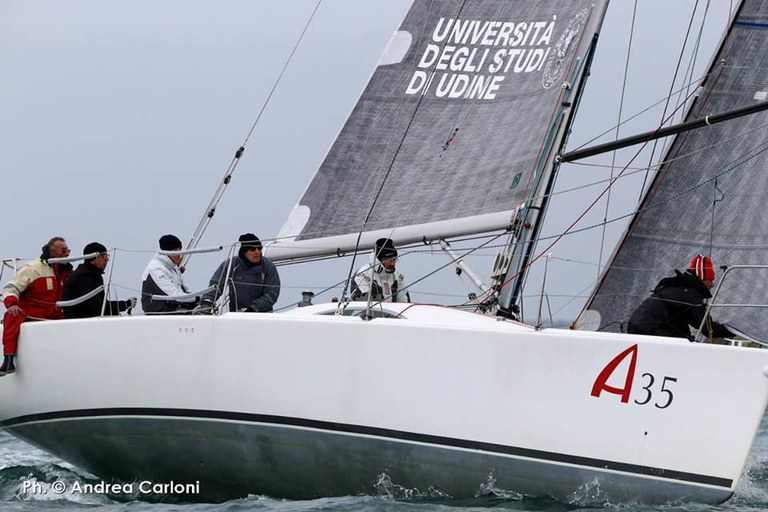
\includegraphics[scale=0.5]{william_b}
		\caption[Barca a vela Williab B]{Barca a vela da regata \textit{William B} \cite{william_b}}
		\label{figura:william_b}
	\end{center}
\end{figure}

\chapter{Architettura hardware e software}

\section{Hardware}
\subsection{Premessa}
Per l'implementazione dell'architettura hardware è stata utilizzata della componentistica semplice ed economica. Principalmente l'hardware utilizzato è un \textit{Raspberry} ed un \textit{ricevitore GPS}, per ricevere le coordinate geografiche della barca durante la competizione.

\subsection{Raspberry}
A bordo della barca è stato installato un \textbf{Raspberry Pi 3 Model B}, un computer di dimensioni ridotte (\textit{single board computer}) che non necessita di eccessivi consumi di energia elettrica e dal costo contenuto. La particolarità di non avere della componentistica di alto livello permette di eseguire un qualsiasi sistema operativo basto su kernel Linux, fornendo un enorme vantaggio dal punto di vista del consumo energetico. Essendo la barca a vela il contesto in cui viene utilizzata questa \textit{single board}, non vi è la possibilità di fornire grandi quantità di energia per sostenere il carico energetico di hardware di alto livello. Pertanto la durata della batteria è un aspetto di fondamentale importanza.

\newpage
Il modello del Raspberry in questione ha le seguenti caratteristiche:
\begin{enumerate}
	\item CPU Quad Core 1.2GHz Broadcom BCM2837 a 64bit
	\item 1GB di RAM
	\item Modulo WLAN BCM43438 e \textit{Bluetooth Low Energy} (BLE) integrato
	\item 10/100 Fast Ethernet
	\item 2 porte USB 2.0
	\item Uscita video HDMI
	\item Lettore schede Micro SD integrato dove risiede il sistema operativo
	\item Porta di alimentazione Micro USB
\end{enumerate}

Il Raspberry deve ospitare un'applicazione server che fornirà dei servizi ai client, comunicare con i vari sensori installati nella barca a vela e mantenere attiva una rete WiFi a cui i vari client possono connettersi per accedere ai servizi del server. Quindi, il Raspberry ha anche il ruolo di \textit{access point wireless}.

\begin{figure}
	\begin{center}
		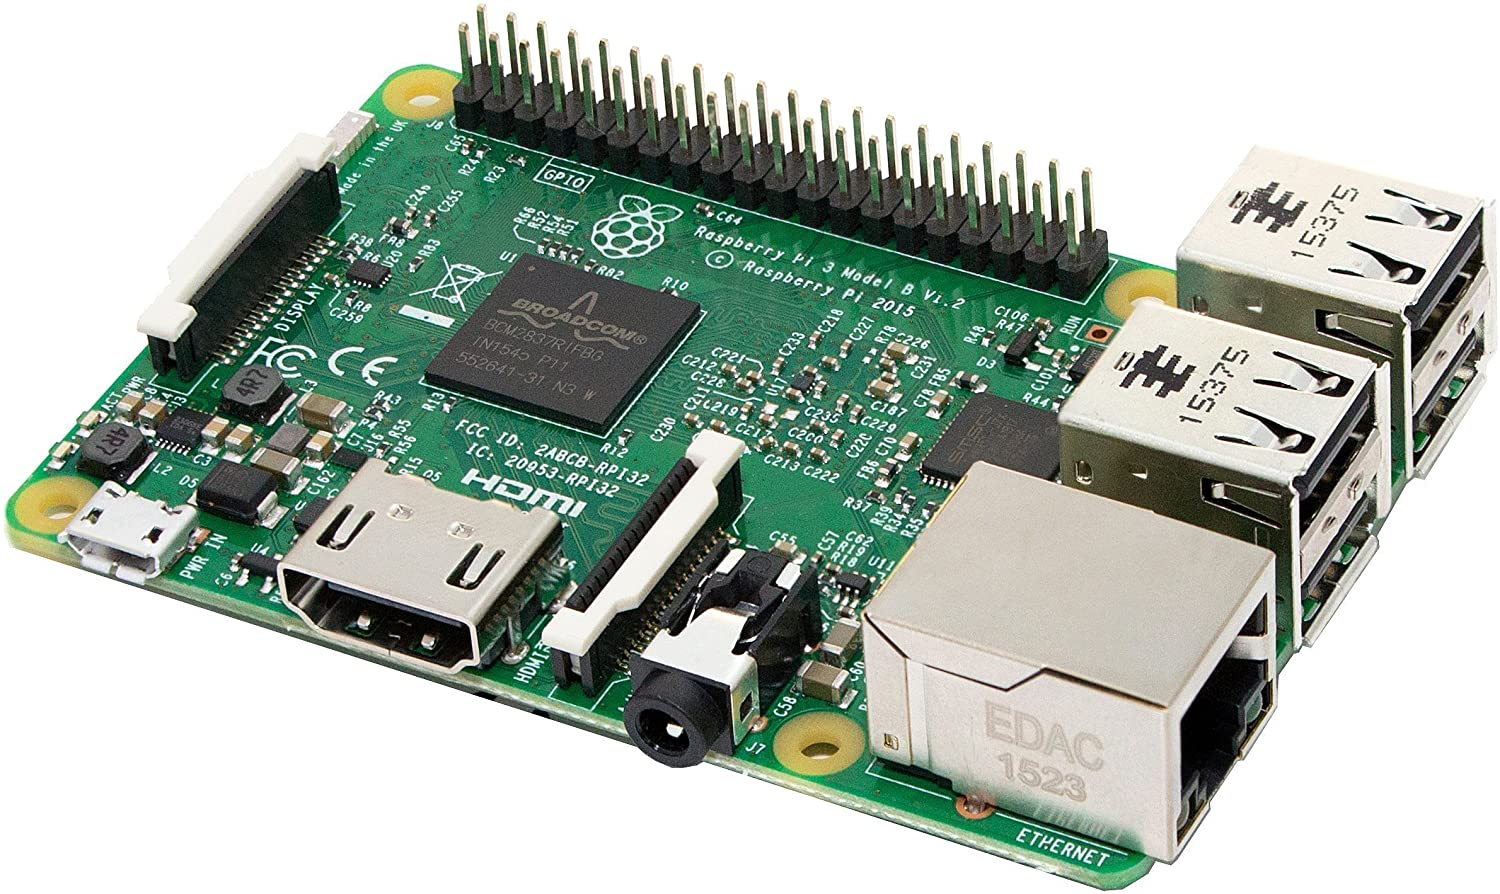
\includegraphics[scale=0.2]{raspberry}
		\caption[Raspberry Pi 3 Model B]{Raspberry Pi 3 Model B.}
		\label{figura:raspberry}
	\end{center}
\end{figure}

\newpage
\subsection{Ricevitore GPS}
Per tracciare la rotta da percorrere è necessario ottenere le coordinate geografiche, fornite tramite il \textit{servizio GPS} \cite{gps}. Pertanto viene utilizzato un ricevitore GPS a basso costo, collegabile via USB al Raspberry. L'utilizzo del GPS risulta essere lo strumento ideale in questo contesto, in quanto, trovandosi in un'ampia area, gli eventuali errori vengono mitigati e non compromettono la precisione della posizione determinata.
\begin{figure}
	\begin{center}
		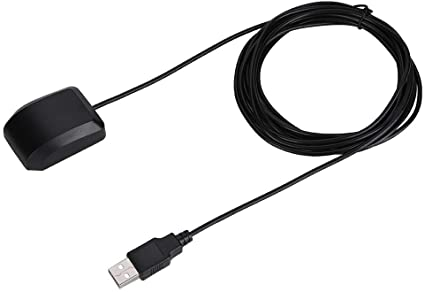
\includegraphics[scale=0.6]{gps_usb}
		\caption[Ricevitore GPS]{Ricevitore GPS collegabile via USB.}
		\label{figura:gps_usb}
	\end{center}
\end{figure}

\section{Software}
\subsection{Modello architetturale}
Per questo progetto si è deciso di utilizzare un'architettura \textbf{Client-Server}. È un modello architetturale per sistemi distribuiti dove le funzionalità che offre il server sono presenti sotto forma di servizi disponibili ai client. I client accedono al server per usufruire dei servizi offerti.

Il principale vantaggio che si può trarre da questa architettura è la possibilità di accedere al server da più postazioni. In questo progetto risulta molto utile accedere al server da postazioni differenti o supportare connessioni multiple (utilizzare l'applicazione da mobile e l'applicazione Web).
L'indipendenza tra server e client è un importante vantaggio in quanto è possibile apportare delle modifiche ad uno dei due \textit{attori} senza influire sull'altro o su altre parti del sistema. I client devono conoscere il nome del server disponibile (o i nomi dei server nel caso in cui ve ne siano più di uno) e i servizi che offre. Il server invece non necessita di conoscere i client che si connettono a lui ed è in grado di gestire un numero arbitrario di connessioni. I client usufruiscono dei servizi offerti dal server tramite un protocollo di \textit{richiesta-risposta}, dove un client invia una richiesta e rimane in attesa di una risposta da parte del server. In particolare, il protocollo implementato per questo progetto permette la comunicazione tra i due attori tramite l'utilizzo delle \textit{socket}, un'astrazione che fornisce una API per l'architettura TCP/IP.

Lo svantaggio maggiore di questa architettura è la suscettibilità ad attacchi \textit{Denial-of-Serevice} (\textit{DoS}), oltre ad essere soggetta ad eventuali guasti del server. Inoltre le prestazioni possono essere imprevedibili in quanto dipendono sia dal carico della rete, sia dal carico di lavoro che il server deve sostenere.

È necessario prestare attenzione alla separazione tra il concetto di \textit{server fisico} e l'\textit{applicazione server}: il server fisico è una macchina fisica dotata di componentistica in grado di poter supportare le funzionalità tipiche di un server (grandi quantità di risorse di calcolo e di memoria). L'applicazione server è un software che fornisce dei servizi per i client e che può essere installato indipendentemente che il dispositivo sia un server fisico o un normale personal computer. Un discorso analogo può essere fatto anche per i client.

\subsection{Funzionalità implementate dal server}
\subsubsection{Comunicazione con i sensori}
Una delle funzionalità principali che il server implementa è la comunicazione con i sensori installati sulla barca a vela. In particolare, il server raccoglie i dati in tempo reale, leggendoli in \textit{modalità seriale}. La comunicazione tra il server ed i sensori avviene tramite la centralina \textbf{NMEA 183 Interface Output}, sviluppata dall’azienda \textit{NKE Marine Electronics}. Questa centralina opera da intermediario tra i dati rilevati dai sensori ed il Raspberry. In particolare, la centralina converte i dati che provengono dai sensori in formato \textit{ASCII} e li trasmette tramite la porta seriale al server, utilizzando il formato \textbf{NMEA 0183}, un formato standard di comunicazione utilizzato per applicazioni nautiche e per dati GPS.

\newpage

\subsubsection{Manipolazione dei dati raccolti}
Una volta prelevati i dati dai sensori, questi vengono memorizzati in un \textit{buffer}, pronti per essere inviati ad un qualsiasi client che ne fa richiesta. I dati vengono parsati in JSON, un formato per lo scambio di informazioni molto usato per le comunicazioni di rete. Inoltre, i dati prelevati dai sensori vengono utilizzati per la generazione di file di \textit{log}, necessari per eseguire delle simulazioni a terra.

\subsection{Argos}
Sul Raspberry è stato installato il software \textbf{Argos}. Argos è un'applicazione lato server che offre dei servizi ai client che vi si connettono. È scritto in \textit{C} e permette di raccogliere i dati registrati dai sensori installati sulla barca. Questi dati vengono notificati dai sensori al server ad intervalli regolari, in modo da averli sempre aggiornati ai fini delle decisioni che devono essere prese durante la competizione. Per rendere disponibili questi dati ai client, Argos apre una socket nella rete locale e rimane in ascolto sulla porta \verb|4545|: appena un client si connette, il server restituisce il set di dati formattato in JSON e chiude la comunicazione, ritornando in ascolto sulla porta.

\subsubsection{Prima versione}
La prima versione dell'applicazione server rimaneva in ascolto su due porte: la porta \verb|4545| e la porta \verb|4546|. Tramite la porta \verb|4545|, venivano accettate le richieste dei client che volevano ottenere le informazioni riguardo ai sensori della barca in formato JSON. Tramite la porta \verb|4546|, invece, i client potevano inviare delle richieste in formato JSON, differenti rispetto alle prime. Queste richieste indicavano al server di svolgere determinate azioni. Quindi, le richieste venivano elaborate dal server e la risposta veniva fornita tramite la porta \verb|4545|.

\subsubsection{Seconda versione}
La seconda versione del server ha rimosso la funzionalità della porta \verb|4546|, ovvero, è stata tolta la possibilità di ricevere dei dati da parte dei client, di elaborarli e di restituire una risposta. Quindi, l'ultima versione permette soltanto di connettersi alla porta \verb|4545| per ottenere i dati provenienti dai sensori della barca, parsati e formattati dal server.

\begin{figure}
	\begin{center}
		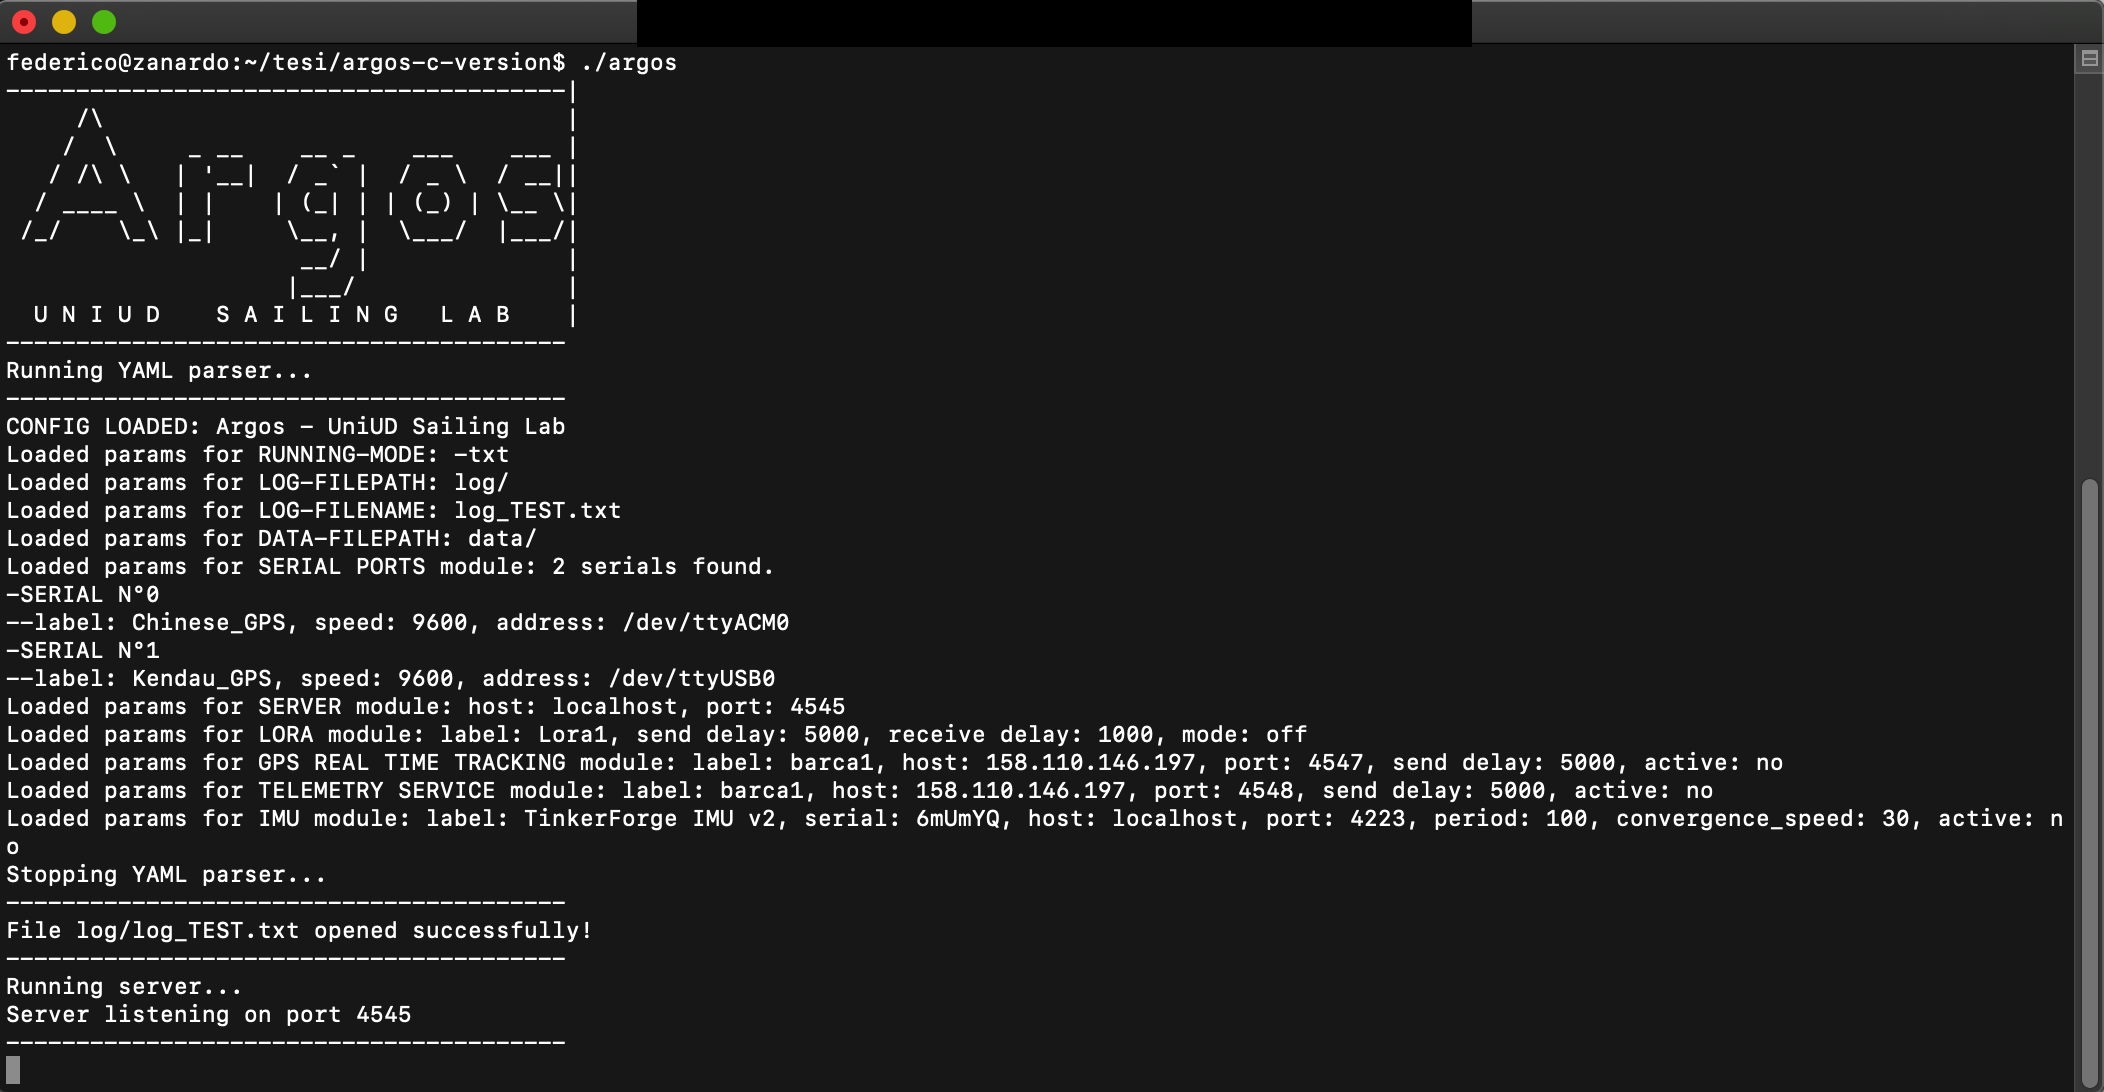
\includegraphics[scale=0.4]{argos}
		\caption[Argos]{La seconda versione del server \textit{Argos} in esecuzione.}
		\label{figura:argos}
	\end{center}
\end{figure}

\newpage

\subsubsection{Dati rilevati dai sensori ed elaborati dal server}
I dati che vengono rilevati dai sensori e poi inviati al server, vengono salvati su un file nel formato JSON. I sensori notificano periodicamente il server della disponibilità di nuovi dati: in questo modo l'utente avrà a disposizione sempre un set di dati aggiornati. Oltre ai dati forniti dai sensori, il server mette a disposizione degli ulteriori dati necessari per effettuare il \textit{debugging}. Tali dati per il debugging vengono forniti dalla socket insieme a tutti gli altri dati dei sensori, senza la necessità di dover effettuare delle particolari richieste.

Di seguito verrà fornita una descrizione di alcuni dei dati che vengono raccolti dai sensori e poi resi disponibili dal server:
\begin{enumerate}
	\item \textbf{A.W.S.} (Apparent Wind Speed): identifica la velocità del vento apparente o stimata;
	\item \textbf{A.W.A.} (Apparent Wind Angle): identifica l’angolo del vento apparente;
	\item \textbf{S.O.G.} (Speed Over Ground): indica la velocità effettiva della barca esente dagli effetti delle correnti marine;
	\item \textbf{C.O.G.} (Curse Over Ground): indica la direzione vera della barca, esente dagli effetti delle correnti marine. Rappresenta la rotta che sta percorrendo la barca;
	\item \textbf{M.H.} (Magnetic Heading): identifica il valore della direzione, segnalata dalla bussola di bordo;
	\item \textbf{S.O.W.} (Speed Over Water): rappresenta la velocità della barca sull’acqua;
	\item \textbf{T.W.S.} (True Wind Speed): indica la velocità attuale del vento;
	\item \textbf{T.W.A.} (True Wind Angle): rappresenta l'angolo percepito del vento;
	\item \textbf{I.H.} (Imu Heading): rappresenta la direzione data dalla IMU, l'angolo rispetto al Nord magnetico;
	\item \textbf{C.ANG.} (Calypso Ang): indica l'angolo con cui il vento arriva sullo strumento di misurazione \textit{Calypso}, ovvero, l’angolo misurato in base alla tacca segnata sullo strumento;
	\item \textbf{C.AMP.} (Calypso Amp): identifica la forza del vento, misurata in nodi, dallo strumento \textit{Calypso};
	\item \textbf{NWANG}: indica l'angolo del vento rispetto al Nord magnetico. È dato somma di \textit{IMU Heading} e \textit{Calypso Ang};
	\item \textbf{LATITUDE}:  latitudine;
	\item \textbf{LONGITUDE}: longitudine.
\end{enumerate}

Nell'applicazione finale, questi dati vengono distribuiti nelle varie schermate. Alcune schermate mostreranno un piccolo set di questi dati per focalizzarsi su determinati aspetti come la navigazione, il vento o le coordinate GPS. La dashboard invece offre un quadro generale della situazione, illustrando tutti i dati appena descritti.

I dati elencati non sono tutti quelli che vengono forniti dalla socket: i dati illustrati sono soltanto quelli che vengono utilizzati all'interno dell'applicazione.

\subsection{Neptune}
\subsubsection{Premessa}
Il lavoro riguardo alla realizzazione dell'applicazione Web è stata dapprima affrontata dallo studente \textit{Davide D'Osvaldo}. Un miglioramento di tale applicazione è stato effettuato prima da \textit{Edoardo Polce} e successivamente da \textit{Alessandro Martin}. Il mio lavoro ha preso in considerazione la versione dell'applicazione di quest'ultimo.

Lo sviluppo dell'applicazione per dispositivi Android è stato effettuato dallo studente \textit{Andrea Mazzocut}, di cui farò riferimento in questa sezione.

\subsubsection{Obiettivo dell'applicazione}
\textbf{Neptune} è un'applicazione lato client che permette di connettersi al server (tramite una socket alla porta \verb|4545|). Il client deve necessariamente essere connesso alla rete WiFi creata dal Raspberry. Ad intervalli regolari, l'applicazione interroga la socket per ottenere dei dati riguardanti i sensori installati sulla barca. Questi dati, in formato JSON, vengono mostrati in un'apposita interfaccia grafica. Nel corso di questo progetto, diversi studenti hanno partecipato alla realizzazione di differenti tipologie di applicazioni, per usufruire dei servizi offerti dal server Argos.

\subsubsection{Applicazione web}
\begin{figure}
	\begin{center}
		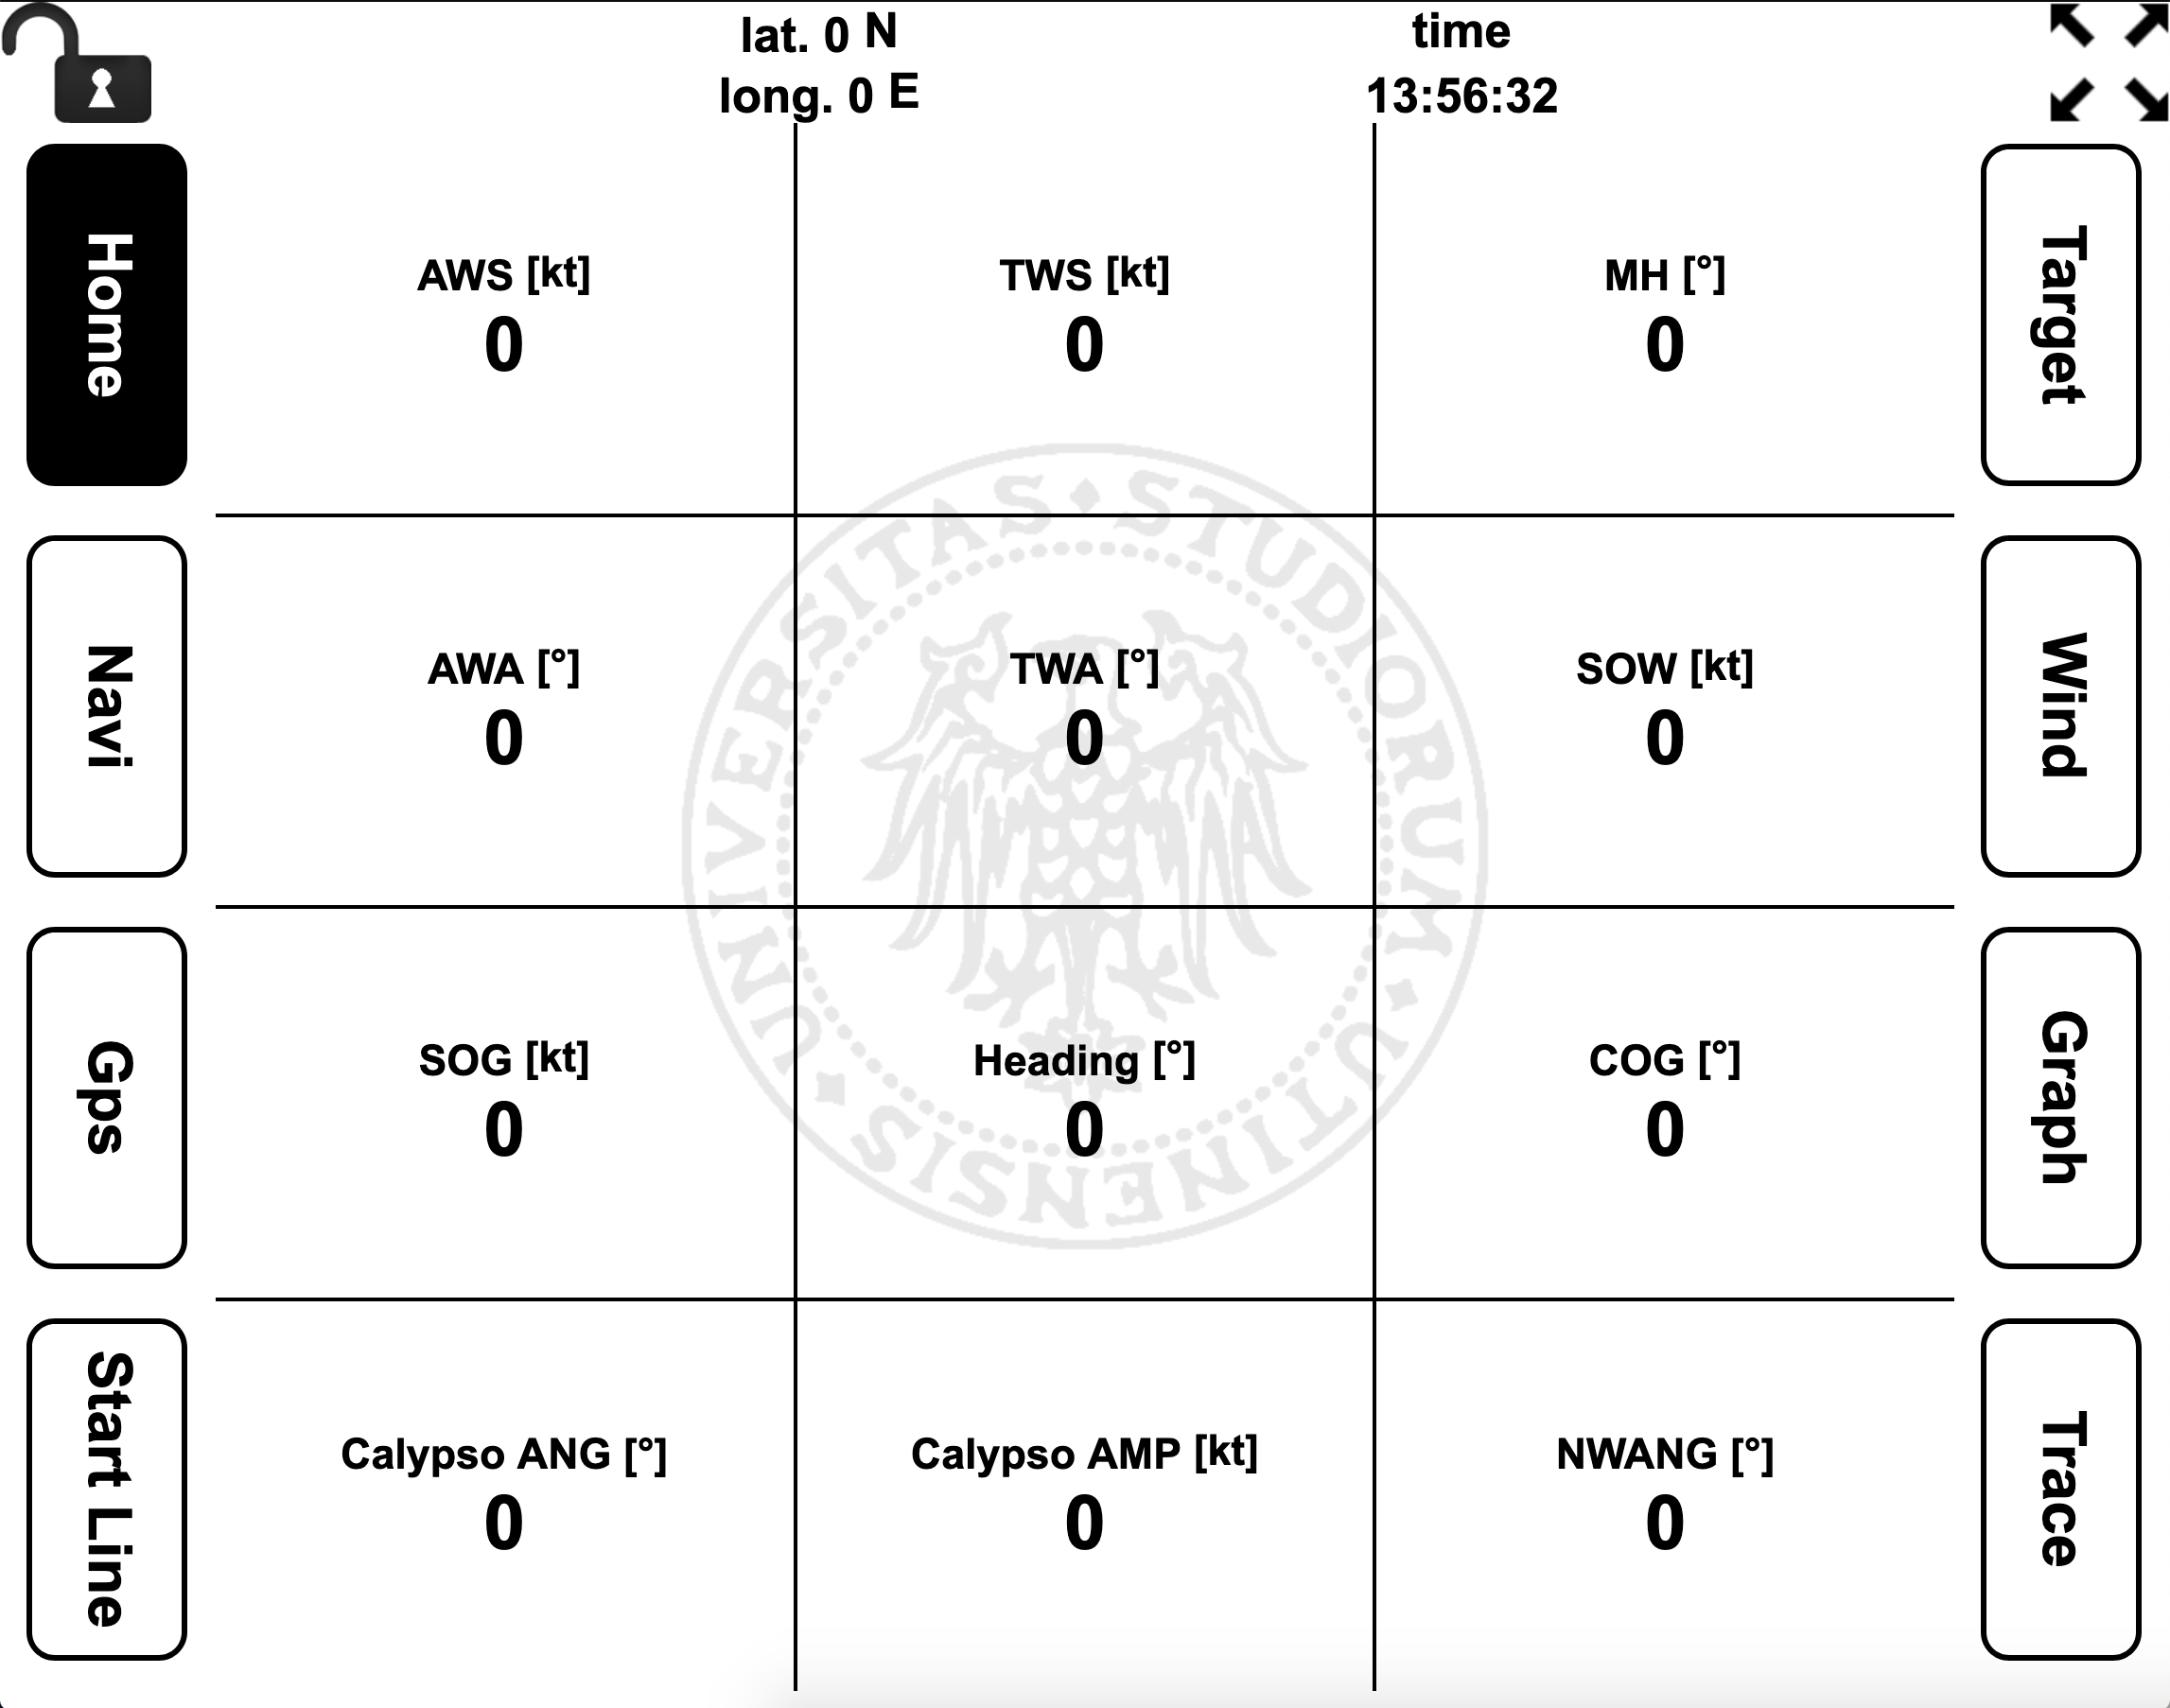
\includegraphics[scale=0.3]{neptune_web}
		\caption[Neptune - versione Web]{Schermata Home dell'applicazione Neptune nella versione Web.}
		\label{figura:neptune_web}
	\end{center}
\end{figure}

L'obiettivo di questa applicazione è la creazione di una sorta di \textit{computer di bordo} per essere utilizzato dall'equipaggio durante la competizione. L'accesso a Neptune è permesso a qualsiasi dispositivo che possa connettersi via wireless al Raspberry, in quanto l'applicazione è accessibile tramite il \textit{browser}.

L'applicazione è costituita da diverse schermate: in particolare, è possibile notare una schermata che presenta una serie di dati per avere un quadro generale di tutti i segnali provenienti dai sensori e delle altre schermate che permettono di monitorare dei dati specifici. Così facendo è possibile avere sia una panoramica generale dei dati rilevati dai sensori, sia un focus preciso su un piccolo set di dati.

Il software è stato sviluppato in HTML, CSS e JavaScript per la parte \textit{frontend}, mentre per la parte \textit{backend} è stato utilizzato PHP. Tuttavia questa versione dell'applicazione porta con sè diversi svantaggi, sopratutto a livello di uso pratico. Durante la regata, vengono utilizzati dei dispositivi mobili come smartphone e tablet, in modo da poterli maneggiare facilmente in ogni situazione e in ogni condizione. Di conseguenza, dispositivi di dimensioni maggiori rispetto a quelli citati sopra non vengono presi in considerazione. Per usufruire dell'applicazione Web è necessario quindi collegarsi via browser al sito web che ospita l'applicazione. L'esperienza utente per questa tipologia di software e per i dispositivi utilizzati non è ottimale, in quanto non vengono sfruttate appieno tutte le funzionalità native del dispositivo mobile.

\subsubsection{Applicazione Android}
Lo sviluppo di un'applicazione \textit{nativa} per dispositivi mobili con sistema operativo \textit{Android} è stata presa in considerazione per cercare di sopperire agli svantaggi della versione Web. L'applicazione nativa non ha l'intento di estendere o introdurre delle nuove funzionalità al servizio offerto, bensì l'intento è quello di rendere il servizio più facile da utilizzare e più reattivo in termini di prestazioni. Infatti, così facendo, è possibile sfruttare appieno le caratteristiche dei dispositivi mobili, permettendo un uso più naturale del servizio e riducendo anche i consumi delle risorse del dispositivo.
Sulla base di queste considerazioni, è possibile personalizzare meglio il servizio: ad esempio, in questa versione dell'applicazione, è stato possibile introdurre la funzionalità per cambiare l'indirizzo IP, quando lo si necessita. Nella versione Web questo poteva essere fatto soltanto dal programmatore che ha realizzato l'applicazione. La funzionalità appena descritta non ha un'importanza maggiore rispetto alle altre già esistenti, ma aiuta a migliorare il servizio nel caso in cui si renda necessario dover svolgere un'operazione di questo genere.

\begin{figure}[htp]
	\centering
	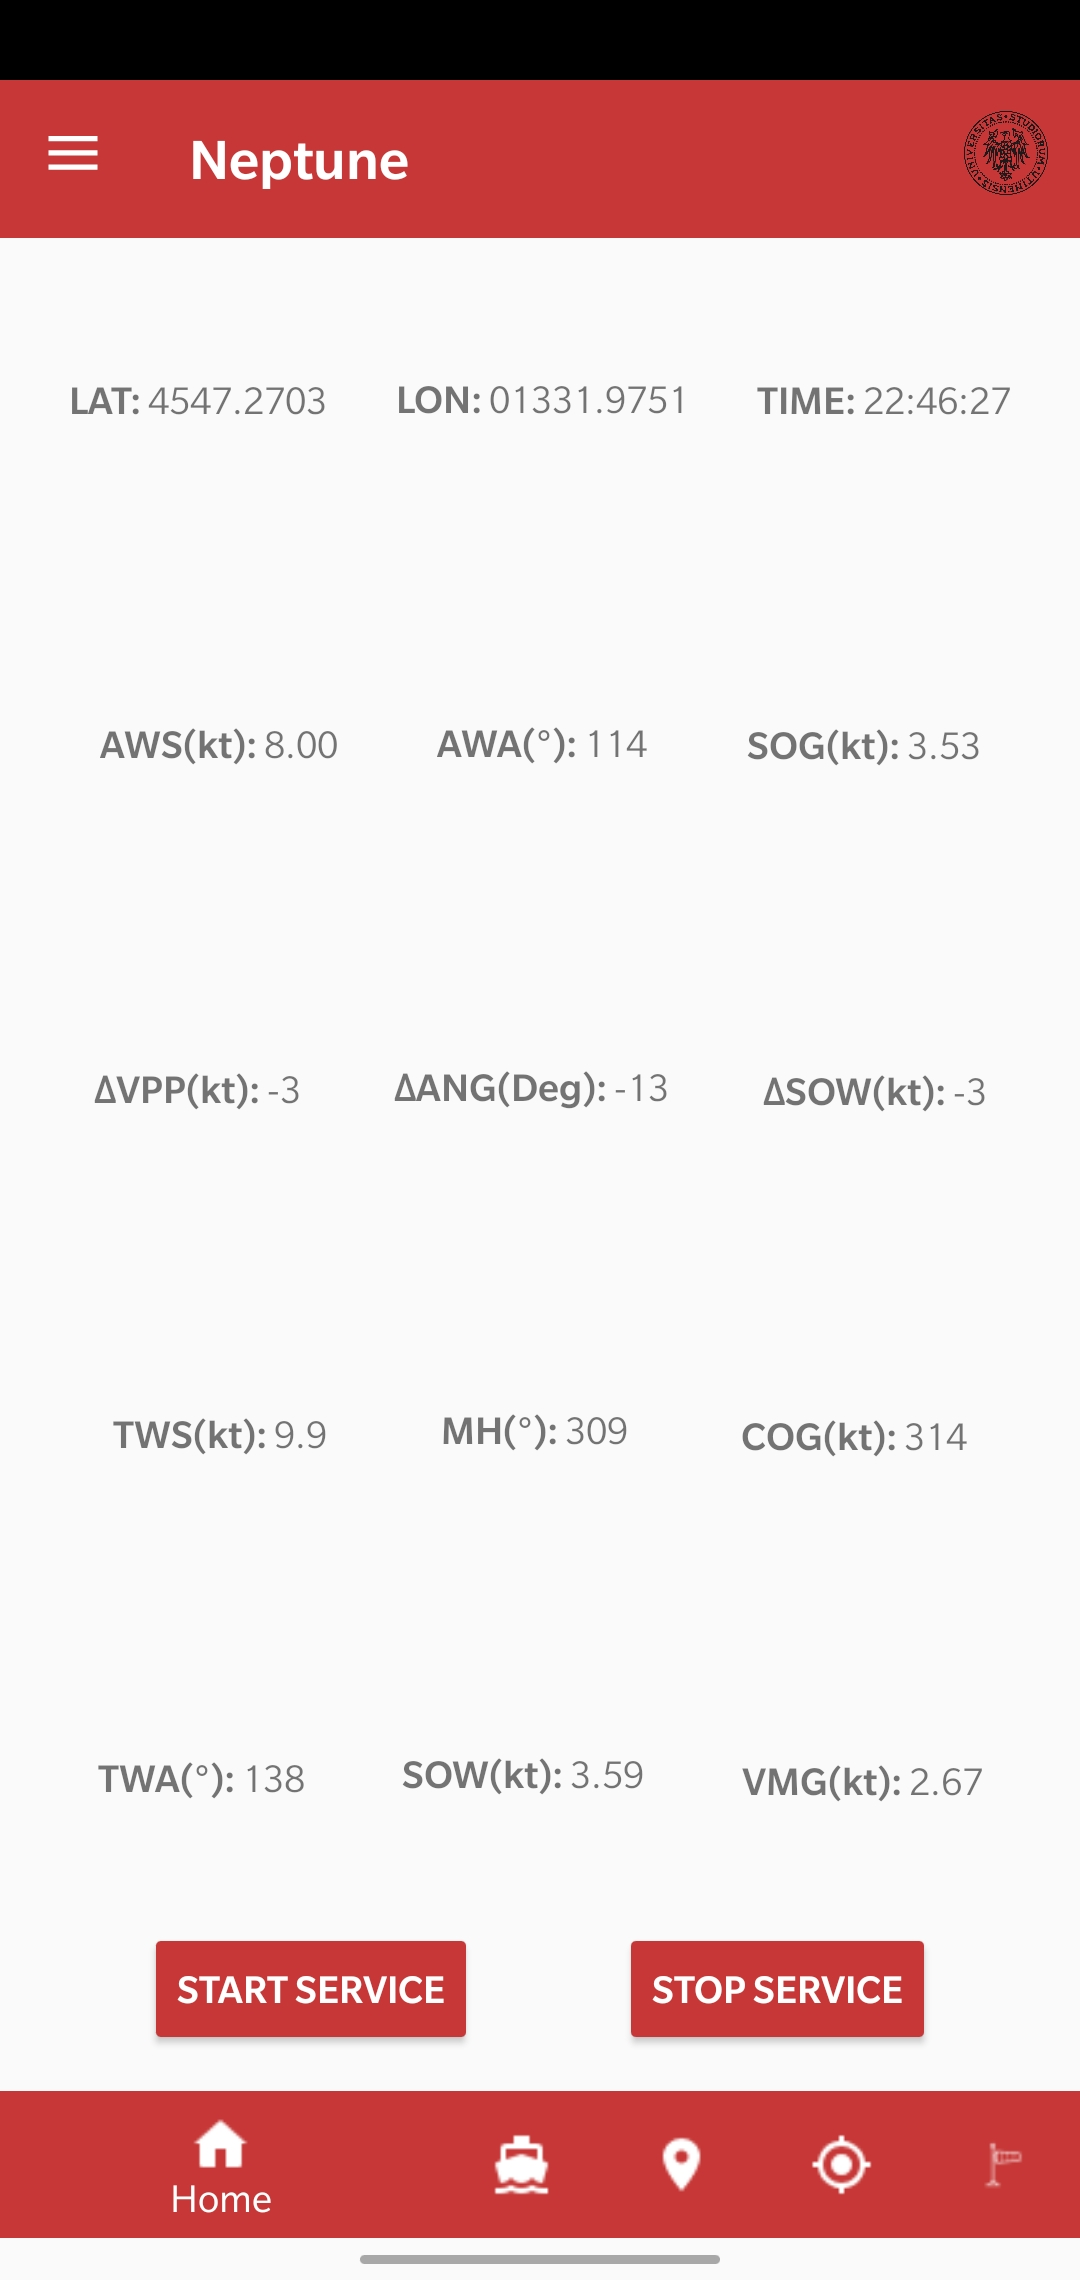
\includegraphics[scale=0.12]{neptune_home}\hfill
	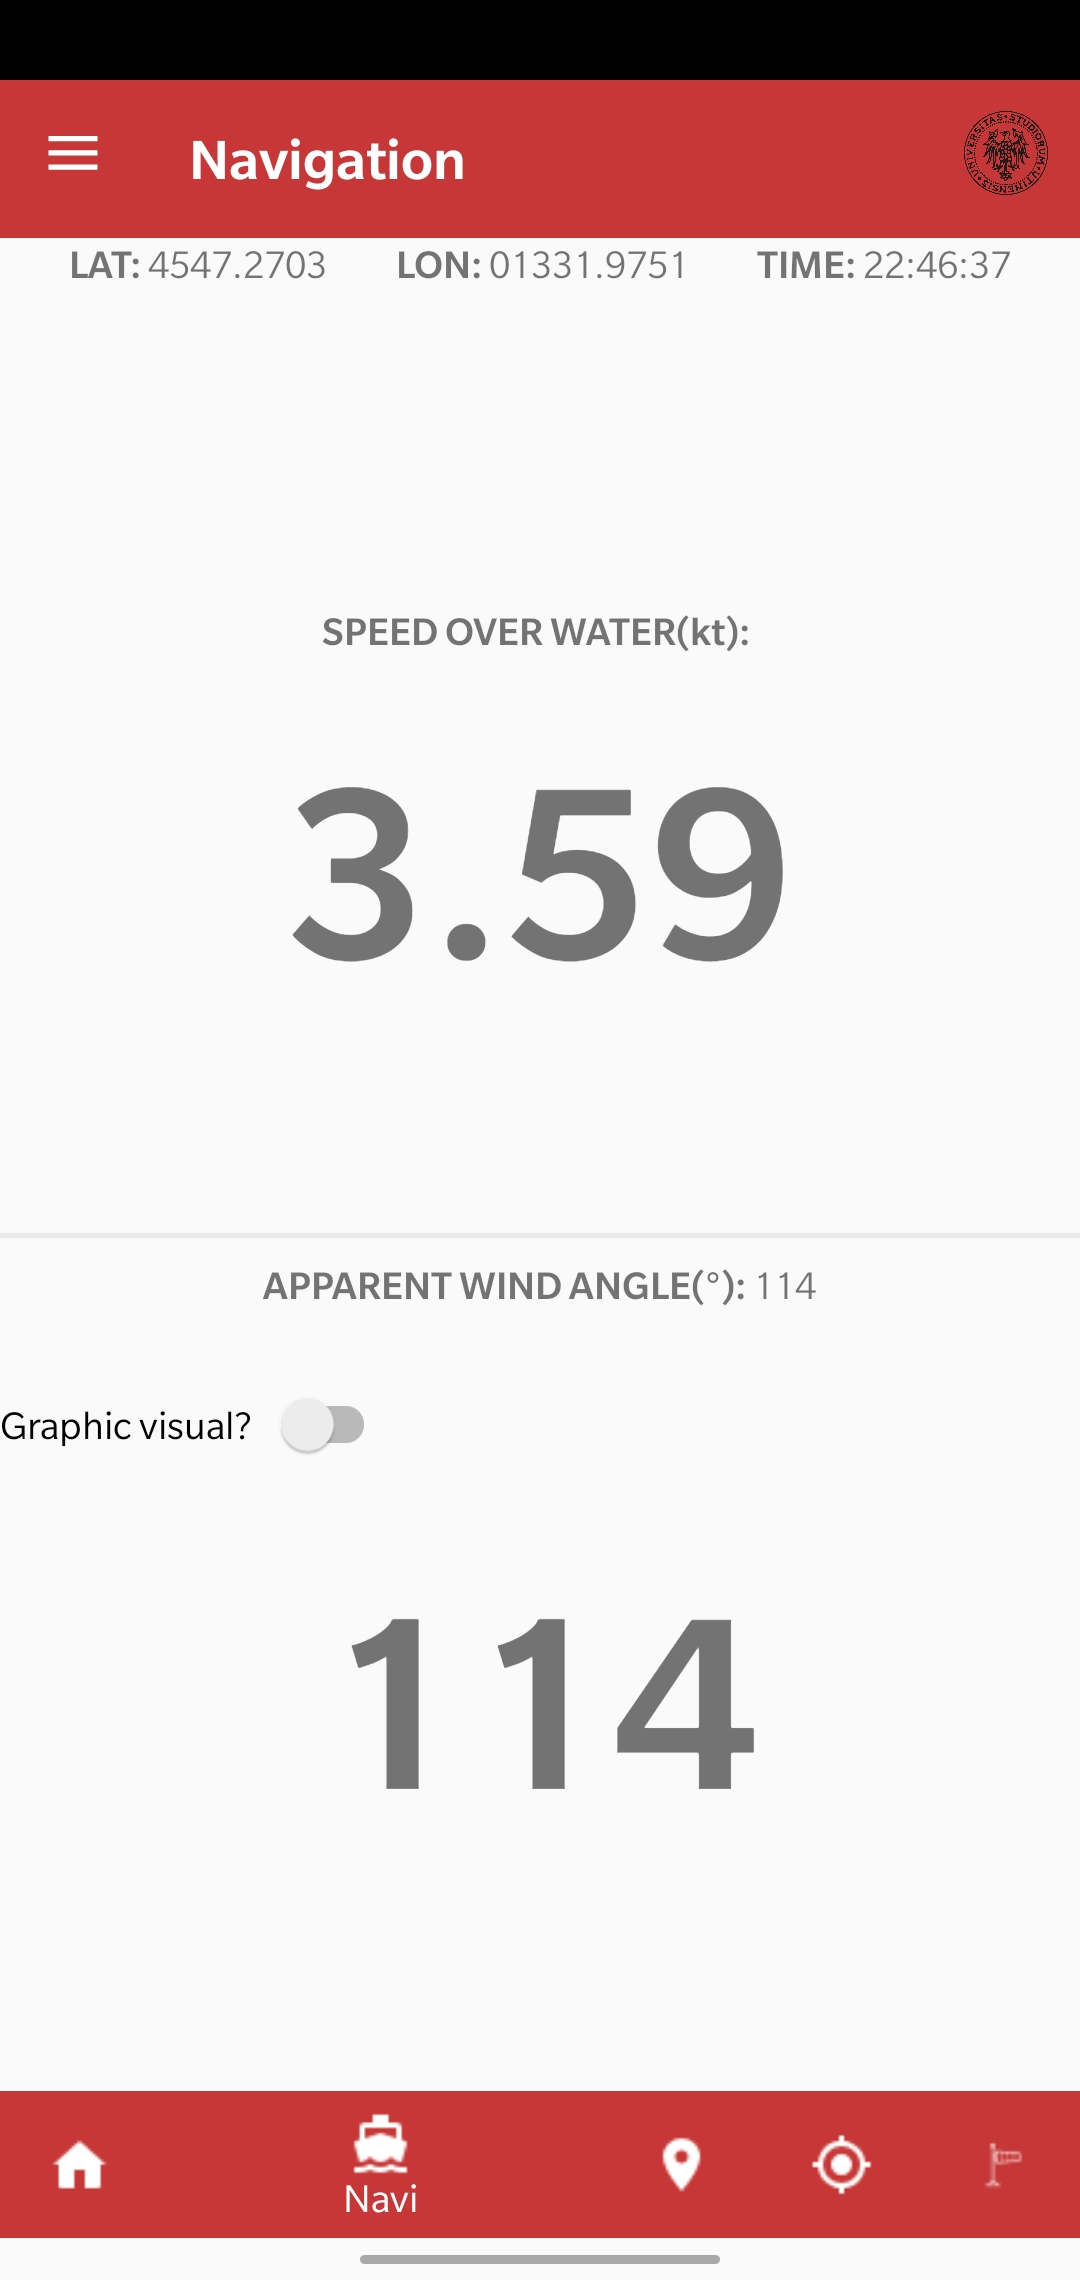
\includegraphics[scale=0.12]{neptune_navigation}\hfill
	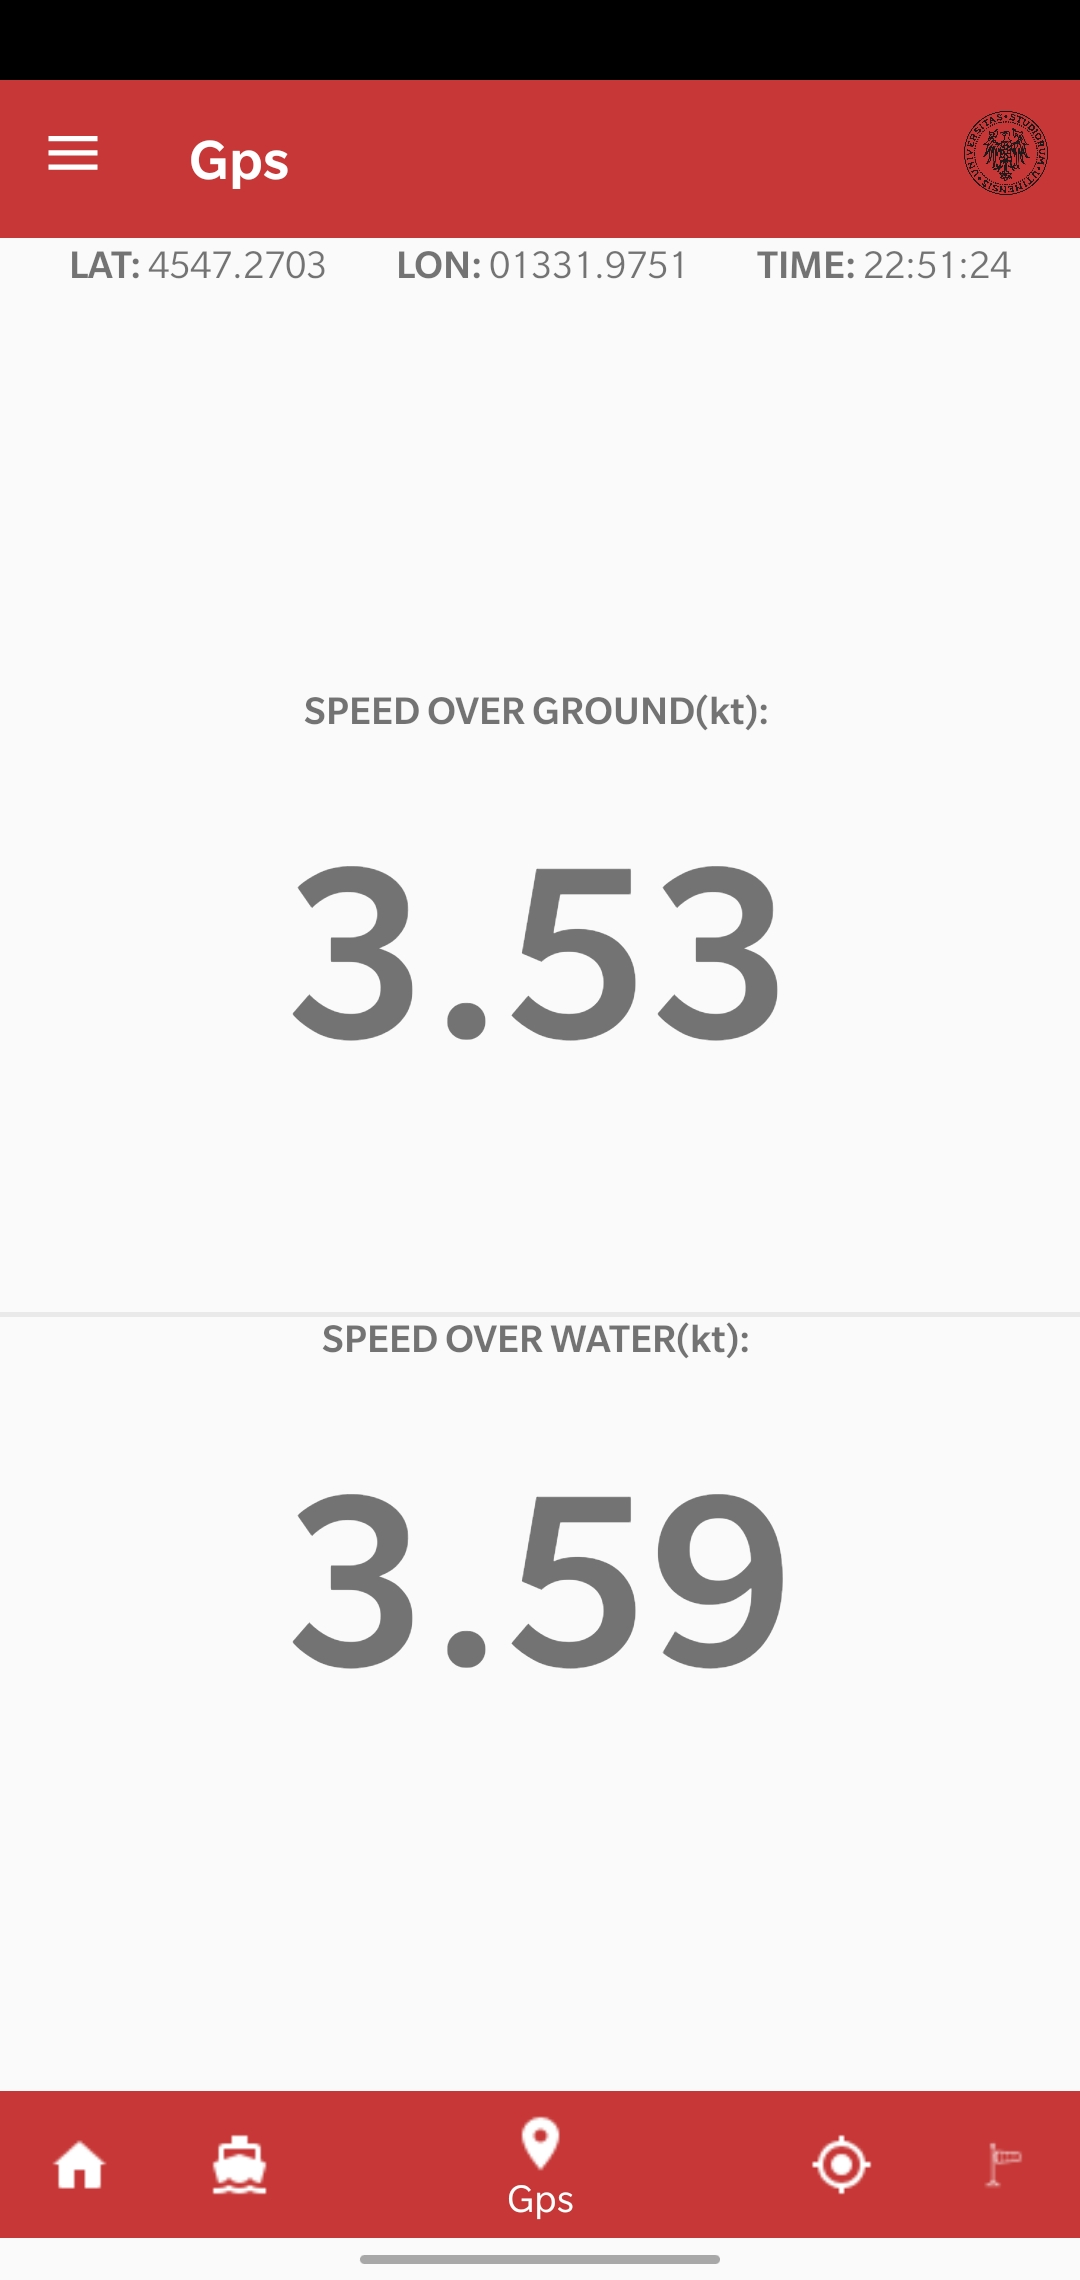
\includegraphics[scale=0.12]{neptune_gps}
	\caption[Neptune - versione Android]{Alcune schermate dell'applicazione Android: schermate Home, Navigation e GPS (in ordine da sinistra).}\label{xyz}
\end{figure}



\chapter{Classificazione delle applicazioni mobili}
\section{Introduzione}
In questo capitolo si procede all'esplorazione delle varie metodologie di sviluppo di applicazioni nate in questo ultimo decennio. Si vanno ad analizzare pregi, difetti e peculiarità di ogni approccio. Inoltre, si va a considerare quali possono essere i contesti d'uso in cui è preferibile utilizzare una metodologia rispetto ad un'altra.

\section{Native}
Nel corso di questo ultimo decennio, lo sviluppo di applicazioni \textit{mobile} ha subito una profonda trasformazione ed evoluzione. Inizialmente lo sviluppo di applicazioni era possibile soltanto con i linguaggi di programmazione supportati dal sistema operativo. Di conseguenza era necessario conoscere le varie piattaforme (\textbf{Android}, \textbf{iOS} e \textbf{Windows Phone} sono i principali sistemi operativi per mobile che hanno caratterizzato questo mercato in questo decennio). Inoltre, per sviluppare applicazioni che potessero utilizzare appieno sia l'hardware che il software del dispositivo, era ed è tuttora necessario avere un'approfondita conoscenza di tutti i sistemi operativi su cui si vuole distribuire la propria applicazione. 

Al giorno d'oggi i due competitor che coprono la quasi totalità del mercato mobile sono Android e iOS \cite{statistiche_os_mobile}. Essendo progettate per uno specifico sistema operativo, queste applicazioni sono ottimizzate e riescono a garantire delle prestazioni ottimali. Il linguaggio di programmazione utilizzato offre una serie di funzionalità e librerie che permettono il completo accesso alla componentistica hardware del dispositivo (ad esempio, l'accesso ai sensori).

Possiamo osservare le considerazioni appena fatte da un punto di vista economico: se si vuole sviluppare un'applicazione e la si vuole distribuire sia su dispositivi Android che iOS, l'azienda dovrà assumere (almeno) uno sviluppatore per ogni sistema operativo. Più aumenta la complessità dell'applicazione, più persone dovranno essere aggiunte ai due team di sviluppo. Concettualmente, è necessario sviluppare \textit{due codici sorgenti} della \textit{medesima applicazione} per poterla distribuire su due \textit{store} differenti (\textit{Play Store} per Android e \textit{App Store} per iOS). Questo comporta ad assumere diversi sviluppatori per realizzare quella che è concettualmente una singola applicazione.

Da un punto di vista tecnico, lo sviluppo della medesima applicazione da parte di due team che operano su ambienti differenti, portano a numerose difficoltà a livello di progettazione dell'applicazione e a livello organizzativo. Ad esempio, a parità di conoscenze ed esperienza dei singoli componenti dei team di sviluppo sulla piattaforma in cui operano (la conoscenza delle \textit{hard skills}), l'introduzione di una nuova funzionalità può risultare semplice da sviluppare per un team, ma può diventare fonte di difficoltà per l'altro team. Questo può provocare dei rallentamenti nel rilascio della nuova funzionalità o può generare delle \textit{asimmetrie} tra le due applicazioni, ovvero, una funzionalità può essere disponibile per un sistema operativo ma non nell'altro.

Volendo riassumere in punti i vantaggi e gli svantaggi dell'approccio nativo:
\begin{enumerate}
	\item I vantaggi sono:
	\begin{enumerate}
		\item Le applicazioni native sono più veloci e più affidabili in termini di prestazioni. In generale sono più efficienti avendo a disposizione l'accesso alle risorse del dispositivo rispetto ad altri approcci di sviluppo;
		\item Utilizzano l'interfaccia utente del dispositivo nativo, offrendo agli utenti un'esperienza più ottimizzata;
		\item Avendo il pieno accesso all'hardware del dispositivo, può essere utilizzata un'ampia gamma di funzionalità, come ad esempio il giroscopio, la bussola, il Bluetooth, la posizione GPS ed altro ancora.
	\end{enumerate}

	\item Gli svantaggi sono:
	\begin{enumerate}
		\item La non portabilità: una volta realizzata un'applicazione per uno specifico sistema operativo, questa non può essere utilizzata in altre piattaforme. Questo implica il bisogno di assumere diversi sviluppatori con conoscenze specifiche su uno specifico sistema operativo per poter realizzare l'app. Le principali conseguenze di questo svantaggio sono l'aumento dei costi (sia in termini di tempo che economici) e la difficoltà nel manutenere l'applicazione;
		\item Simmetria dei codici sorgenti: avendo più codici sorgenti per diversi sistemi operativi, si manifesta la difficoltà di mantenere aggiornati tutti i codici sorgenti nel momento in cui si vuole rilasciare una nuova funzionalità;
		\item Ogni aggiornamento dell'applicazione deve essere scaricato manualmente dall'utente tramite l'apposito store;
		\item L'applicazione contribuisce ad occupare lo spazio di memoria del dispositivo.
	\end{enumerate}

\end{enumerate}

In origine, l'unico linguaggio permesso per la realizzazione di applicazioni per Android era \textbf{Java}. Oggi è possibile creare delle applicazioni anche con \textbf{Kotlin}. Analogamente, per quanto riguarda iOS all'inizio era permesso soltanto il linguaggio \textbf{Objective-C}, mentre, oggi è possibile sviluppare app anche con \textbf{Swift}, un linguaggio sviluppato appositamente dalla casa madre per i suoi dispositivi.

\section{Web App}
Tutte le considerazioni fatte a riguardo l'approccio nativo hanno portato allo sviluppo di applicazioni Web che fossero \textbf{mobile friendly}, ovvero, che potessero essere facilmente utilizzate anche da smartphone. L'intento principale è quello di sviluppare un'applicazione indipendentemente dalla piattaforma su cui verrà ospitata, ovvero, tramite l'utilizzo del \textit{browser}, software installabile in qualsiasi dispositivo. Nonostante il nome possa trarre in inganno, queste applicazioni vengono denominate \textit{Web app}. Le Web app non sono delle vere e proprie app, ma si cerca di rendere \textbf{responsive} il sito web, ovvero, di rendere il sito \textit{mobile friendly}. Per \textit{mobile friendly} si intende che la Web app deve avere un'interfaccia grafica che si adatti alle dimensioni dello schermo in maniera dinamica ed automatica. Sviluppando secondo questa concezione, è sufficiente implementare un unico codice sorgente per distribuire l'applicazione su qualsiasi dispositivo mobile e desktop (\textit{Write once use everywhere}). L'utilizzo di queste applicazioni non comportano ad alcuna installazione e di conseguenza non incideranno sullo spazio di memoria del dispositivo. L'applicazione è sempre aggiornata all'ultima versione perchè è sempre richiesta la connessione ad Internet per poterla usufruire. I costi per lo sviluppo sono abbattuti dal momento che il team che ha realizzato il sito web può anche sviluppare la versione per mobile, senza i problemi di distribuzione su piattaforme diverse.

Tuttavia non è possibile utilizzare appieno le risorse hardware e software che offre il dispositivo e di conseguenza l'ambito di applicazione di questa metodologia di sviluppo risulta essere limitato. 
L'interfaccia grafica e l'esperienza utente sono di basso livello e le applicazioni di questo genere sono molto limitate in termini di funzionalità.

Per realizzare queste applicazioni vengono utilizzati i linguaggi di programmazione per lo sviluppo di siti Web, ovvero, HTML, CSS, JavaScript e PHP.

In conclusione a questa sezione, possiamo notare che l'approccio nativo e quello delle Web app siano \textit{diametralmente opposti}.

\section{Progressive Web App}
Un'evoluzione delle Web app sono le \textbf{Progressive Web App (PWA)}. Sono molto simili alle Web app, ovvero, mantengono alcune caratteristiche come la possibilità di sviluppare un unico codice sorgente per distribuire l'applicazione su qualsiasi dispositivo e la necessità di non doverla installare. Tuttavia, permettono di ricevere delle \textit{notifiche push} e possono essere utilizzate anche in assenza di connessione ad Internet. Le PWA si appoggiano comunque al browser del dispositivo e quindi presentano le medesime limitazioni in termini di accessibilità delle Web app. Ad esempio, è possibile utilizzare il servizio GPS, ma non è possibile accedere alla fotocamera.

Per realizzare queste applicazioni vengono utilizzati i classici linguaggi per lo sviluppo di siti Web, ovvero, HTML, CSS e JavaScript. Per quanto riguarda i framework più comuni vi sono \textbf{Angular} (Google) e \textbf{ReactJS} (Facebook).

\section{Hybrid}
Le \textbf{app ibride} si pongono come un'evoluzione delle Web app e delle PWA e tentano di congiungere i vantaggi dello sviluppo nativo e delle PWA. Vengono create con i medesimi linguaggi per lo sviluppo Web, ma per funzionare necessitano l'installazione di un software sul device (\textit{engine}). Questo software è uno strato che si interpone tra il dispositivo e l'applicazione ed è necessario per l'esecuzione del codice. L'engine permette di utilizzare in maniera più efficiente e profonda l'hardware del device, oltre ad effettuare il \textit{rendering} della grafica. Ad esempio, è possibile realizzare applicazioni che facciano uso di sensori come l'accelerometro e il giroscopio.

Nonostante questi vantaggi, alcune funzionalità non possono essere realizzate e le prestazioni generali (compresa la \textit{User Experience}) sono nettamente inferiori rispetto alle app native. Inoltre, rispetto alle Web app e alle PWA, queste applicazioni devono necessariamente essere pubblicate sullo store per poter essere installate sul dispositivo. 

Il vantaggio fondamentale che si può ottenere è la possibilità di produrre un unico codice sorgente, utilizzando i classici linguaggi per lo sviluppo Web. Così facendo, è possibile distribuire l'applicazione su più dispositivi possibili, abbattendo in questo modo i costi.

I framework più comuni per la realizzazione di app ibride sono \textbf{Ionic} e \textbf{Apache Cordova}.

\begin{figure}
	\begin{center}
		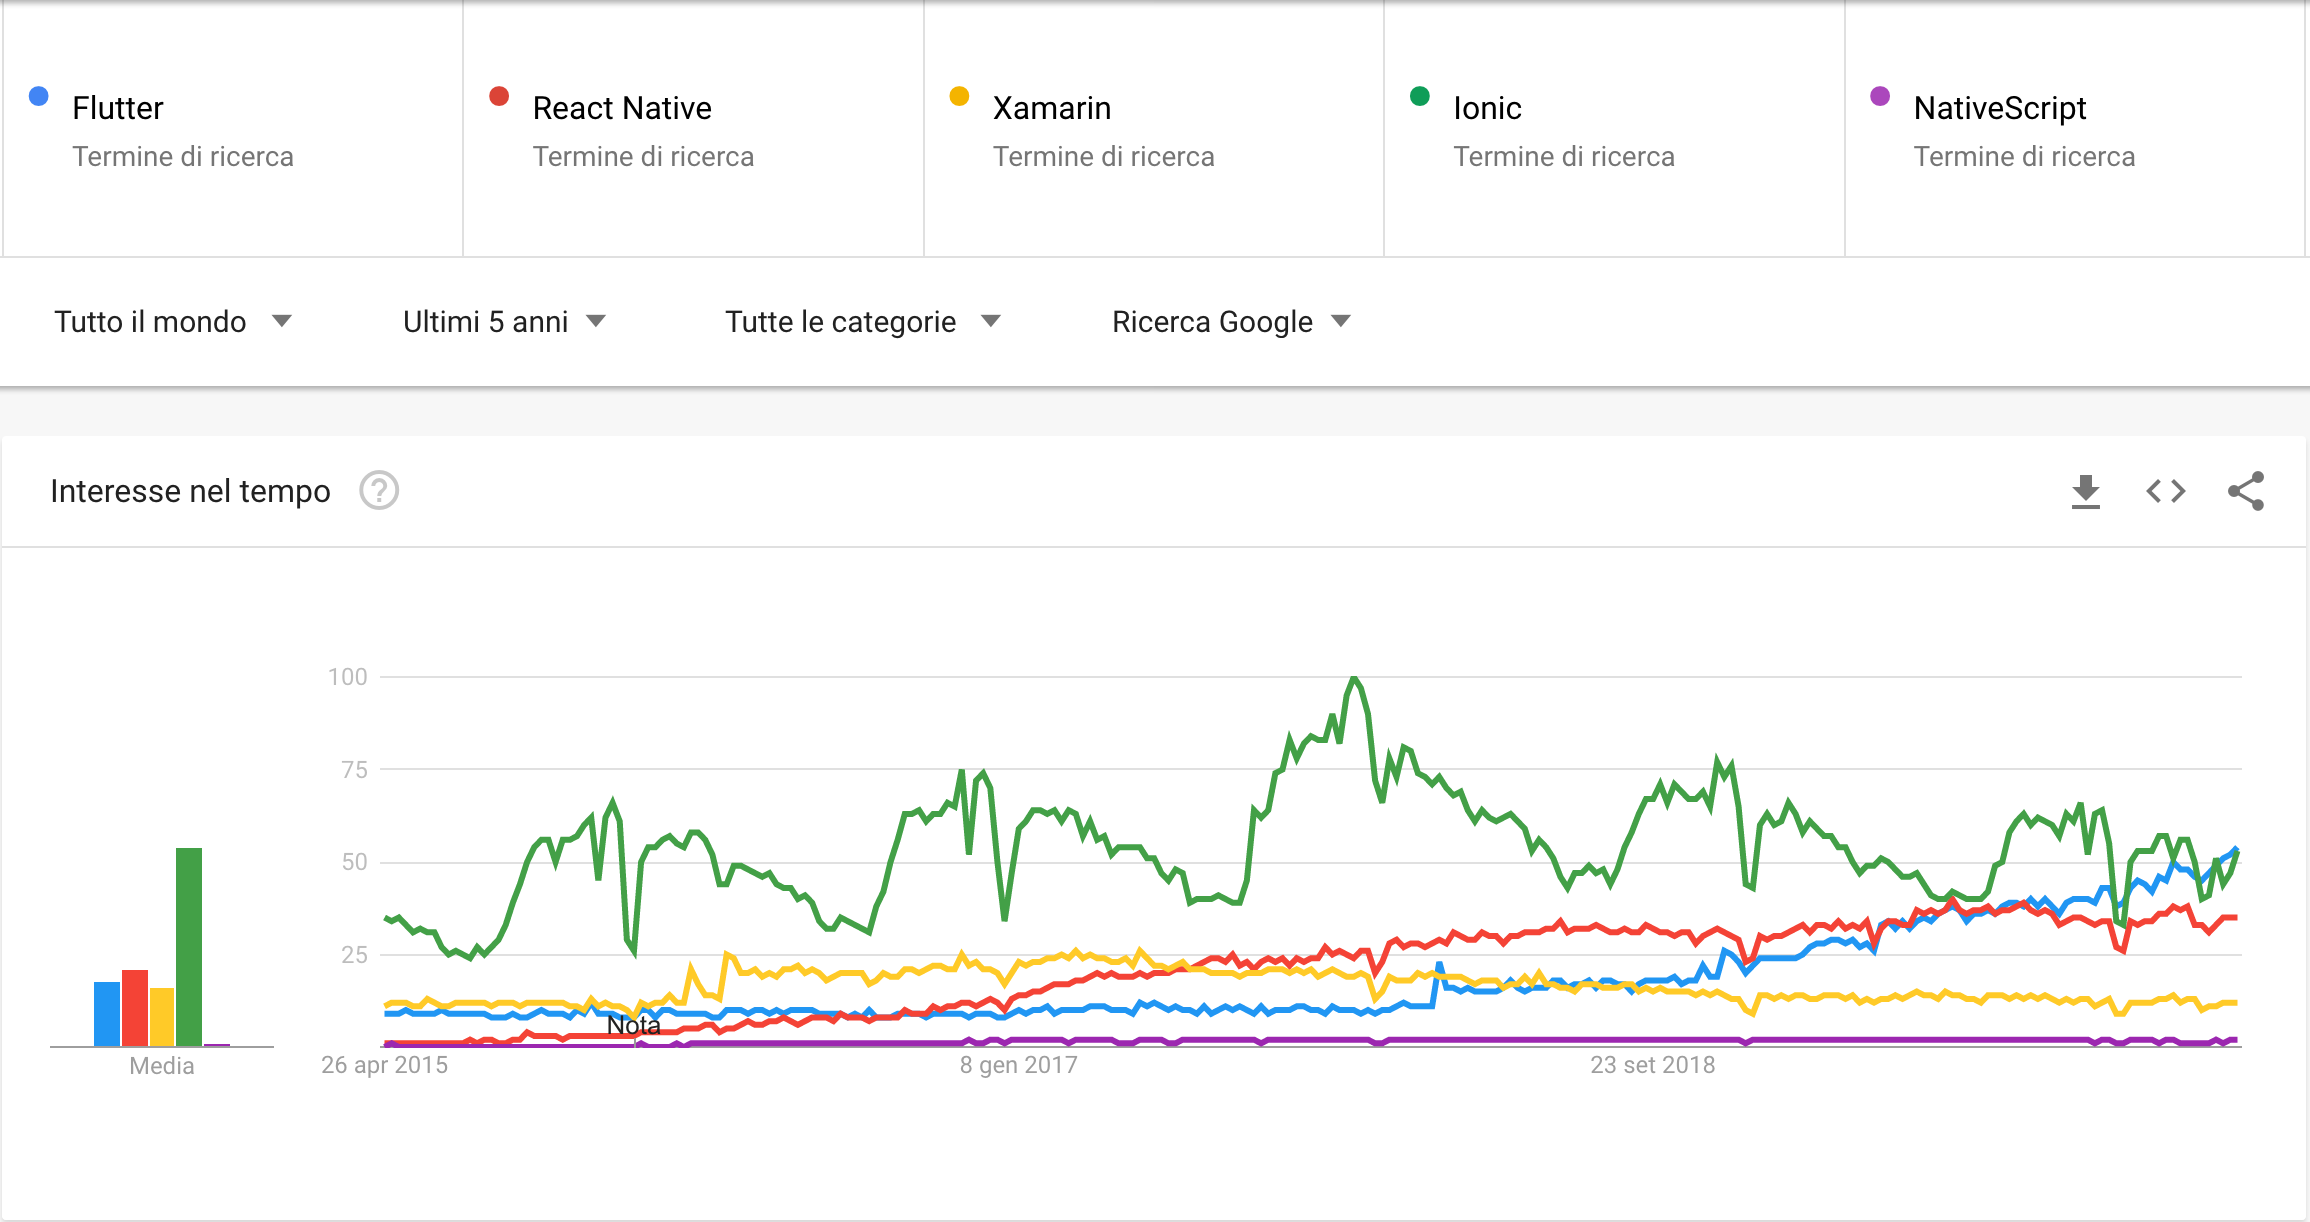
\includegraphics[scale=0.35]{google_trends}
		\caption[Google Trends - Framework Cross-Paltform]{Trends dei framework cross-platform su Google Trends \cite{google_trends}}
		\label{figura:google_trends}
	\end{center}
\end{figure}

\section{Cross-Platform}
Le applicazioni \textbf{cross-platform}, anche dette \textit{platform-independent}, sono applicazioni installabili su dispositivi con sistemi operativi differenti, senza la necessità di produrre un codice sorgente per ogni piattaforma. Sulla base di quanto appena detto, queste applicazioni possono essere confuse per applicazioni ibride, tuttavia hanno delle caratteristiche peculiari che le differenziano. In particolare, le app cross-platform utilizzano un \textit{render engine} nativo che le permette di collegare il codice sorgente direttamente ai componenti nativi dei dispositivi. Così facendo, si aumentano notevolmente le prestazioni ed è possibile sfruttare meglio le risorse hardware rispetto alle applicazioni ibride. Le app ibride fanno uso, invece, di un render creato ad \textit{hoc}. È comunque importante ricordare che soltanto le applicazioni native possono ottenere delle prestazioni ottimali: tutte le altre metodologie di sviluppo cercano di avvicinarsi ma non raggiungono i livelli di un approccio nativo.

In un'applicazione cross-platform è possibile implementare delle funzionalità particolari ed è possibile avere un interfaccia grafica fluida e reattiva, comparabile ad un'app nativa. Questo è l'approccio che più si avvicina alle applicazioni native e pertanto può essere considerata la metodologia più opportuna se si vuole sviluppare un'applicazione senza dover assumere due team di sviluppo differenti e senza sprecare le risorse economiche dell'azienda.

I framework più popolare in questo ambito di sviluppo sono \textbf{React Native} (Facebook), \textbf{Xamarin} (Microsoft) e \textbf{Flutter} (Google).

I linguaggi utilizzati variano da framework a framework: React Native utilizza \textit{JavaScript}, Xamarin permette di scrivere codice in \textit{C\#} (linguaggio proprietario di Microsoft) e Flutter in \textit{Dart} (linguaggio proprietario di Google).

\begin{figure}
	\begin{center}
		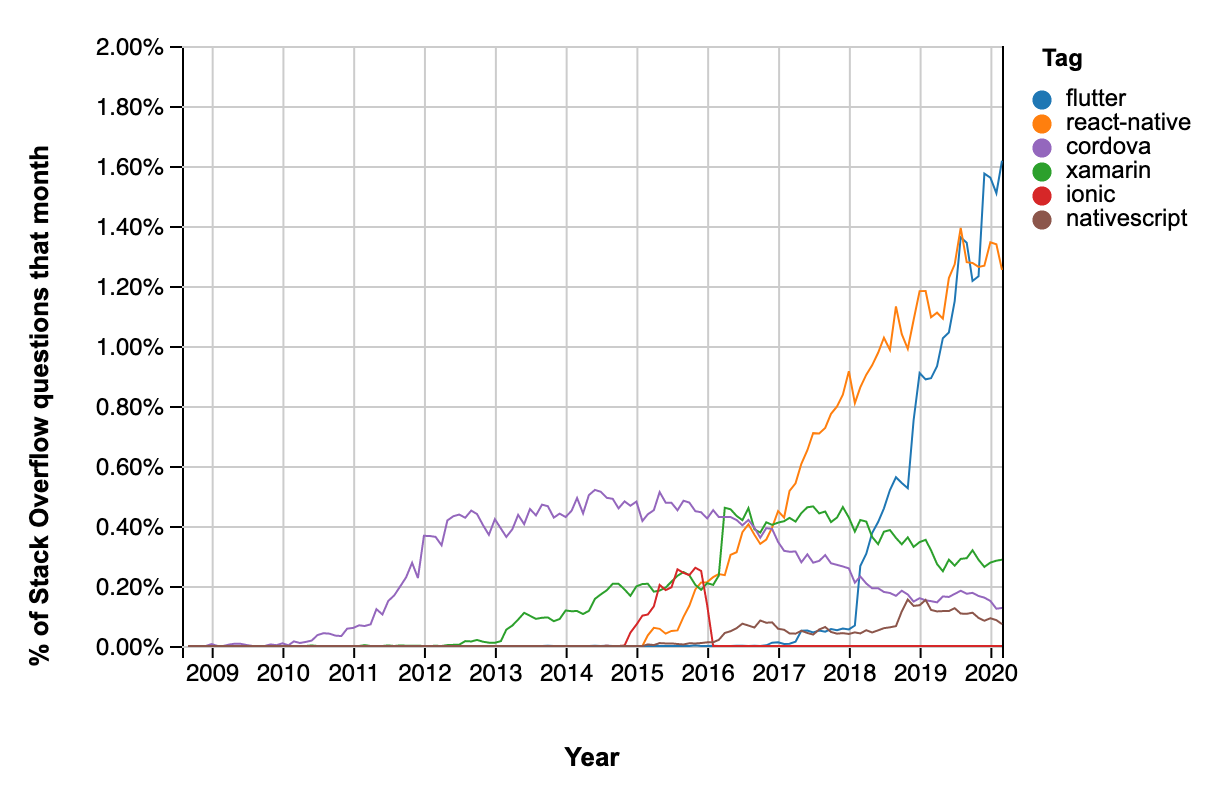
\includegraphics[scale=0.6]{stackoverflow_trends}
		\caption[StackOverflow - Framework Cross-Paltform]{Trends dei framework cross-platform su StackOverflow \cite{stackoverflow_trends}}
		\label{figura:stackoverflow_trends}
	\end{center}
\end{figure}

\section{Considerazioni}
\begin{figure}
	\begin{center}
		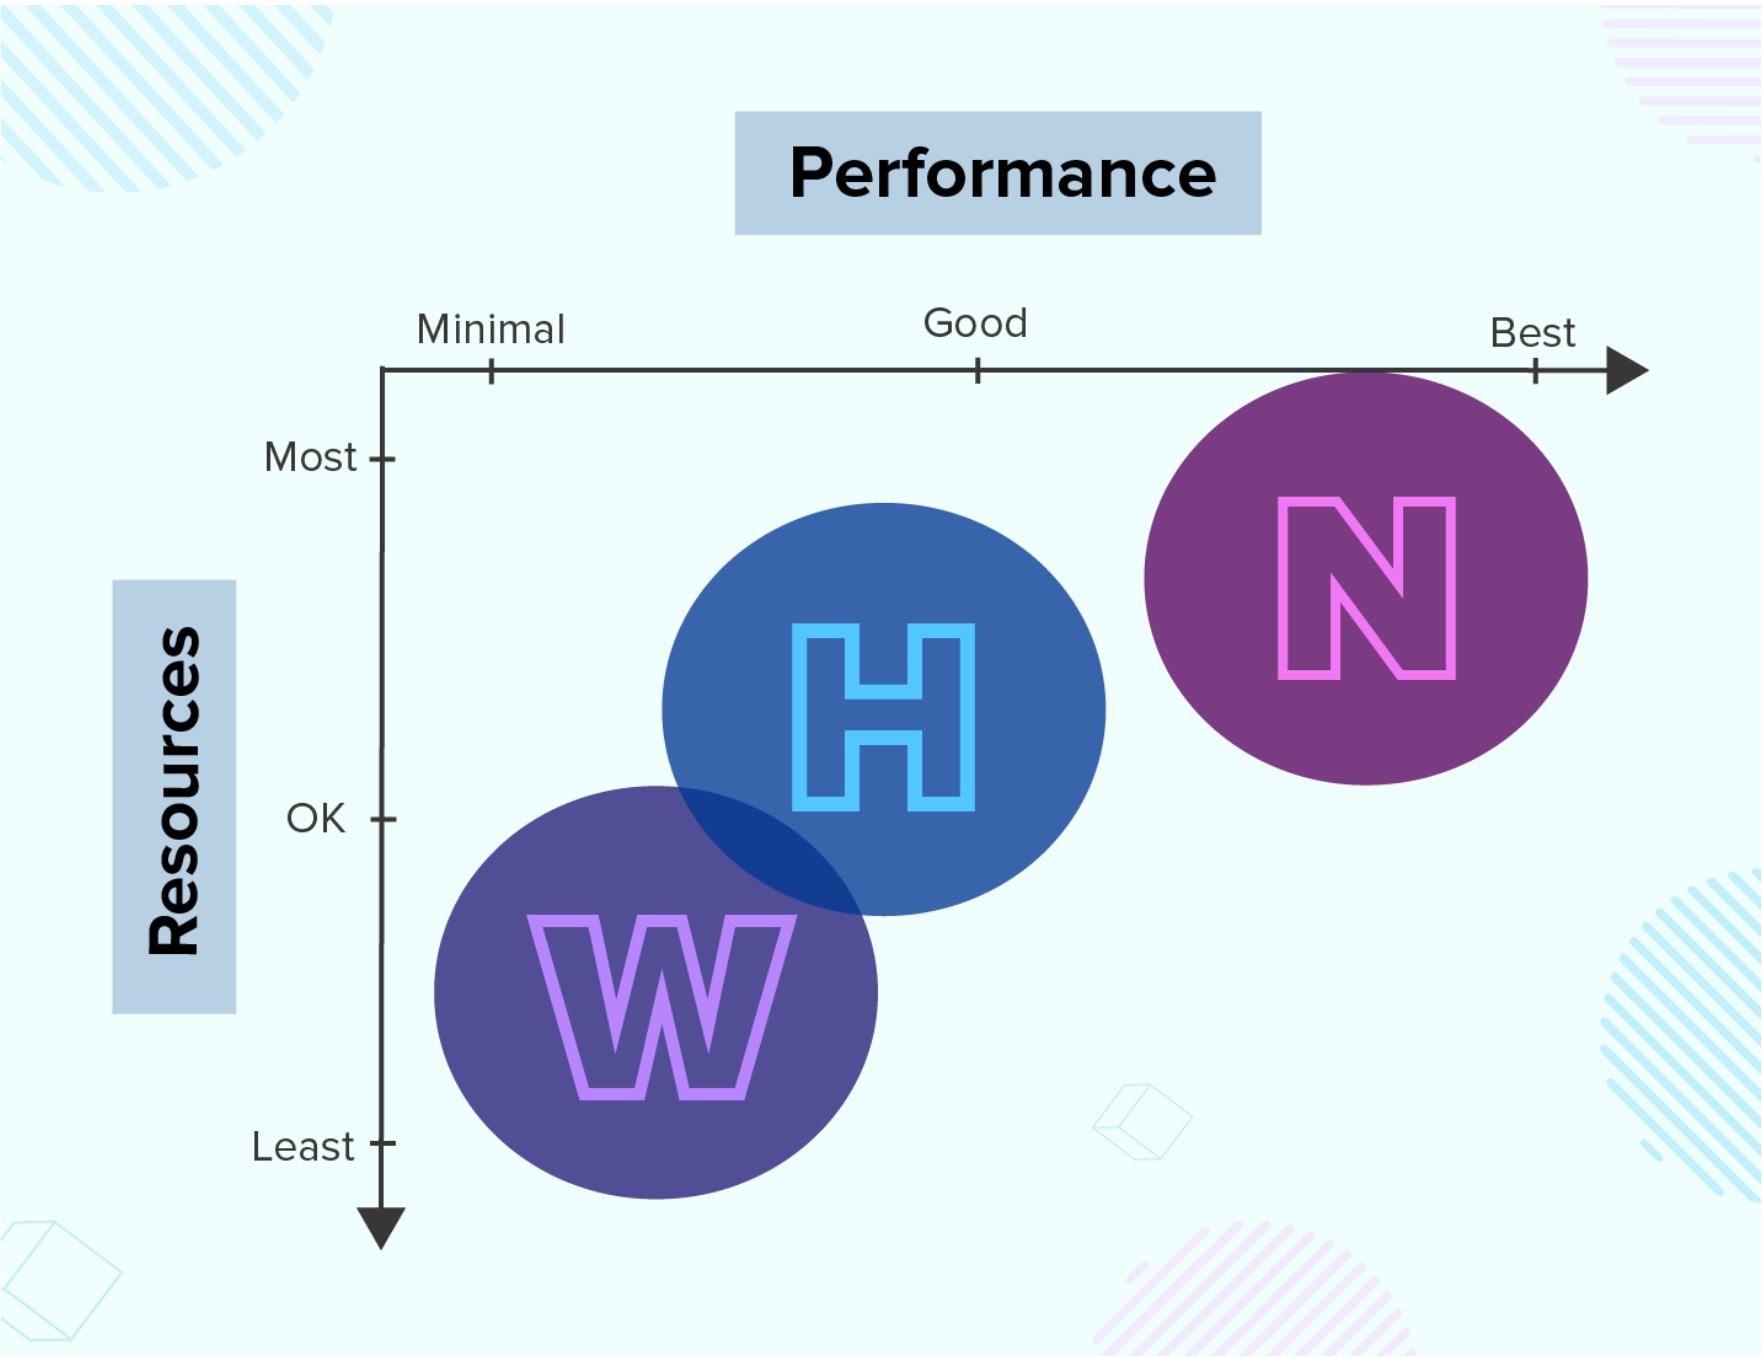
\includegraphics[scale=0.3]{native_hybrid_web}
		\caption[Confronto Native, Hyrbid, Web]{Confronto fra app Native, Hyrbid, Web \cite{grafico_native_hybrid_web}.}
		\label{figura:native_hybrid_web}
	\end{center}
\end{figure}

La decisione di esporre le varie metodologie di sviluppo non è stata presa in modo casuale. Si è voluto mettere in evidenza fin dall'inizio i due approcci in antitesi tra loro, ovvero, le \textit{applicazioni native} e le \textit{Web app}. A partire dalle Web app, si è proceduti verso un progressivo avvicinamento alle applicazioni native, pur tenendo conto che tutte le metodologie presentate, permettono di sviluppare un'app per più sistemi operativi con un unico codice sorgente. In questo modo si è proceduti ad illustrare tutte le possibilità offerte dal mercato per lo sviluppo di applicazioni mobili, considerando aspetti tecnici ed economici.

Dall'analisi effettuata, si possono suddividere gli approcci descritti principalmente in due categorie: \textit{applicazioni native} e \textit{applicazioni multipiattaforma}. Web app, PWA, Hybrid app e Cross-Platform app seguono la filosofia \textbf{\textit{"Write once use everywhere"}} e \textbf{\textit{"Learn once apply everywhere"}}, ovvero, la possibilità di realizzare un unico codice sorgente per distribuire l'applicazione su qualsiasi piattaforma, riutilizzando dei linguaggi di programmazione già esistenti, senza dover imparare uno specifico linguaggio per ogni singolo framework. I principi fondanti di questa categoria di approcci sono:

\begin{enumerate}
	\item \textbf{Manutenibilità}: è sicuramente il vantaggio più importante in termini di tempo e di risorse economiche risparmiate nel processo di realizzazione di un’applicazione. Sviluppando infatti un unico codice per l’applicazione, le attività di manutenzione, correzione e identificazione di eventuali malfunzionamenti risultano essere più veloci;
	\item \textbf{Rapidità di sviluppo}: i tempi di realizzazione, dovendo scrivere un unico codice per tutte le piattaforme, si riducono notevolmente.
\end{enumerate}

In conclusione, possiamo considerare che lo sviluppo di Web app (incluse le PWA) fanno un uso minimale delle risorse offerte dal dispositivo, mentre le applicazioni native fanno un largo uso delle risorse disponibili (Figura 3.3). Le applicazioni ibride si pongono come un compromesso tra la complessità delle applicazioni native e le forti limitazioni delle Web app. Le app cross-platform possono essere collocate vicino alle app native, sia per quanto riguarda la possibilità di utilizzare le risorse del dispositivo e sia dal punto di vista delle prestazioni, ma anche vicino alle Web app per quanto riguarda la semplicità di sviluppo e dell'uso di linguaggi comuni alla programmazione Web (Figura 3.3).

\section{Criteri per la scelta dell'approccio di sviluppo}
In questa breve sezione si prendono in considerazione alcuni degli aspetti e delle motivazioni che possono portare a scegliere un determinato approccio rispetto ad un altro \cite{considerazioni_native_hybrid_cross_platform}.

\subsection{Risorse economiche a disposizione}
Quando si parla dello sviluppo di un'applicazione, un aspetto fondamentale e rilevante è l'\textit{aspetto economico}. Nel contesto di una piccola azienda o di una \textit{startup}, di solito sono disponibili pochi fondi per la realizzazione dell'applicazione. Pertanto, lo sviluppo nativo non è quello consigliato in quanto è necessario trovare uno sviluppatore che sia in grado di programmare sia per Android che per iOS o costruire due team di sviluppo per ogni sistema operativo. È evidente che questo approccio è il più \textit{dispendioso}. In queste situazioni è molto importante concentrare tutti gli sforzi su un'unica piattaforma per ottenere un prodotto finale completo.

Se l'aspetto economico non è un problema, non è necessario comunque sviluppare delle app native. Ad esempio, se un'azienda ha già degli sviluppatori molto esperti in JavaScript, risulta inefficiente non sfruttare le potenzialità di questo team anche per lo sviluppo di un'applicazione per dispositivi mobile. Sopratutto, quando si hanno dei tempi stretti per la realizzazione del prodotto e per la consegna, è consigliato di sfruttare appieno le risorse già presenti nell'ambiente aziendale, senza dover procedere con dei colloqui per assumere altri sviluppatori.

\subsection{Time-to-market e copertura del mercato (reach)}
La creazione di un'applicazione nativa richiede molto più tempo rispetto allo sviluppo di app ibride o PWA. Le tempistiche dettate dal mercato (\textbf{time-to-market}) influenzano le scelte anche di questo genere. Pertanto se si vuole realizzare un prodotto funzionante prima di un \textit{competitor}, è necessario prendere in considerazione anche le vie alternative allo sviluppo nativo. Una volta che il prodotto è stato sufficientemente accettato dal mercato (quando ha superato la cosiddetta \textit{massa critica}), allora si può pensare di ristrutturare l'applicazione e di scegliere altri approcci per gli sviluppi futuri.

Se parliamo in termini di \textbf{reach}, ovvero, di copertura del mercato con il proprio prodotto, è preferibile che l'applicazione possa essere distribuita nel più breve tempo possibile e su più \textit{marketplace} possibili. Questo aspetto invita ad adottare un approccio ibrido o cross-platform, per poter generare con un unico codice sorgente, due versioni dell'app pronte per entrambi gli store.

\subsection{Performance dell'applicazione}
Se le prestazioni sono un fattore fondamentale ed un requisito indispensabile, l'approccio nativo è quello migliore di tutti. Tutti gli altri approcci introducono dell'\textit{overhead}: si pensi ad esempio al bridge JavaScript di React Native per poter utilizzare gli elementi grafici nativi. Un'applicazione nativa ha il pieno accesso alle risorse hardware e software del dispositivo e in questo modo è possibile operare con precisione ed in profondità per ottenere dei vantaggi in termini di prestazioni e di ottimizzazioni.

\subsection{User Experience e interfaccia grafica}
Secondo una statistica del 2018 \cite{tasso_di_abbandono_app}, quasi \textit{una persona su tre} abbandona l'applicazione dopo la prima esperienza. Questo dato stimola la riflessione riguardo alla \textbf{UX} (\textbf{User Experience}) e la \textbf{UI} (\textbf{User Interface}), aspetti fondamentali che devono essere curati se si vuole mantenere una buona \textit{retention} dell'utente nell'applicazione. Le applicazioni native permettono meglio di qualunque altro approccio di realizzare delle animazioni dinamiche e degli scorrimenti fluidi. Dopo le applicazioni native, le app cross-platform sono quelle in grado di riprodurre al meglio una UX vicina a quella che può essere implementata in ambiente nativo. Per quanto riguarda le applicazioni ibride e Web, l'esperienza va a mano a mano a degradarsi.

\subsection{Funzionalità}
Se l'applicazione che deve essere prodotta deve avere delle particolari funzionalità o deve utilizzare determinati sensori, l'approccio migliore è quello nativo perché è possibile accedere completamente a tutte le risorse del dispositivo. A partire dalle applicazioni cross-platform fino alle Web app, la possibilità di interagire con determinati componenti hardware installati nel dispositivo risulta essere sempre più difficile se non impossibile da attuare.

\section{Motivazione della scelta di un framework cross-platform}
Le motivazioni che mi hanno portato a scegliere di utilizzare un approccio cross-platform sono principalmente dovute per ragioni intrinseche del progetto da sviluppare. L'applicazione che deve essere realizzata necessita di visualizzare in \textit{tempo reale} dei dati provenienti da una socket. In particolare si deve tener conto che l'applicazione debba essere \textit{reattiva}. Inoltre si vuole rendere l'applicazione disponibile per più dispositivi mobili, con sistemi operativi differenti. Sulla base di queste considerazioni, l'approccio più plausibile da utilizzare è l'approccio cross-platform, in quanto:
\begin{enumerate}
	\item Permette di creare un'unico codice sorgente per distribuire l'applicazione sia su Android che su iOS;
	\item È l'approccio che più si avvicina a quello nativo, in termini di prestazioni e di accessibilità alla componentistica hardware del dispositivo;
	\item È possibile realizzare un'interfaccia grafica che sia fluida e reattiva, grazie proprio alla maggior vicinanza con l'hardware del device.
\end{enumerate}

La scelta della metodologia cross-platform rappresenta quindi un \textit{trade-off} tra la possibilità di sviluppare un unico codice sorgente sia per Android che per iOS e le prestazioni dell'applicazione.

\chapter{Dart}

\section{Introduzione al linguaggio}
\textbf{Dart} è un linguaggio di programmazione ottimizzato per applicazioni multipiattaforma sviluppato da Google. Questo linguaggio è nato nel 2011 per lo sviluppo di applicazioni Web. Lo scopo di Dart è quello di risolvere i problemi strutturali di \textit{JavaScript} che non possono essere risolti con l'evoluzione del linguaggio stesso. Queste affermazioni sono state scritte in una mail interna di Google, in qui viene definito \textit{Dash} (il nome provvisorio di Dart quando il progetto era ancora in una fase embrionale) il linguaggio che dovrà \textit{"sostituire JavaScript come lingua franca per lo sviluppo web sulla piattaforma web aperto"}\cite{mail_google}.

Dart offre delle prestazioni migliori, rende lo sviluppo più semplice e introduce migliori funzionalità legate alla sicurezza. Nonostante nei primi anni questo linguaggio non riuscì a riscuotere il successo che il team di Google sperava, l'azienda decise di utilizzarlo per lo sviluppo di applicazioni mobile \textbf{\textit{platform-independent}}, ovvero, per l'implementazione del framework \textit{Flutter}. Inoltre, tramite questo linguaggio è possibile creare applicazioni anche per \textit{desktop} (Windows, macOS, Linux/Unix-based e Fuchsia), lato \textit{server} e per dispositivi \textit{IoT}.

Gli obiettivi principali che il team di sviluppo di Google si è preposto di perseguire per la realizzazione di Dart, sono:
\begin{enumerate}
	\item \textbf{Portabilità}: creare un linguaggio strutturato e flessibile per lo sviluppo di applicazioni per il Web e la possibilità di sviluppare applicazioni per tutti i device sul Web.;
	\item \textbf{Produttività}: rendere Dart un linguaggio semplice e familiare ai programmatori, ovvero, con una \textit{curva di apprendimento} bassa. Inoltre deve avere una sintassi chiara e concisa;
	\item \textbf{Velocità}: i costrutti del linguaggio devono fornire delle alte performance ed un avvio veloce delle applicazioni;
\end{enumerate}

In questo capitolo si andranno ad approfondire gli aspetti fondanti del linguaggio e gli aspetti più rilevanti, necessari per la realizzazione del progetto, senza elencare tutte le singole caratteristiche e funzionalità \cite{tour_linguaggio}.

\section{Paradigmi}
Dart è un linguaggio \textit{multiparadigma}, ovvero, è un linguaggio principalmente \textit{orientato agli oggetti} ma offre anche le potenzialità della \textit{programmazione funzionale}, della \textit{programmazione imperativa} e della \textit{programmazione event-driven}. Analogamente al linguaggio Java, fa uso di un \textit{garbage collector}, ovvero, un meccanismo che libera la memoria occupata da oggetti che non sono più utilizzati dal programma. L'utilizzo di più paradigmi permette di ottenere un linguaggio flessibile e che unisce i vantaggi di ogni paradigma \cite{dart_paradigm}.

\subsection{Programmazione reattiva}
Oltre ai paradigmi già citati, Dart integra anche la \textit{programmazione reattiva}, fondamentale per la realizzazione di applicazioni per dispositivi mobile prestanti, veloci ed efficienti \cite{dart_paradigm}. 
Questo paradigma si fonda sulla nozione del cambiamento dei valori nel tempo, a seguito del verificarsi di un evento, e la conseguente propagazione di tali cambiamenti. Diverse fonti forniscono delle definizioni differenti:
\begin{enumerate}
	\item \textbf{Reactive Manifesto}: Reactive Systems are Responsive, Elastic, Resilient, Message Driven \cite{reactive_manifesto};
	\item \textbf{Wikipedia}: Reactive Programming is a programming paradigm oriented around data flows and the propagation of change \cite{reactive_programming_wikipedia}.
\end{enumerate}
Nonostante le differenze, si possono trarre dei concetti che vengono condivisi da entrambe le definizioni. In particolare, i concetti su cui si basa la programmazione reattiva, sono:
\begin{enumerate}
	\item La nozione di \textit{flusso di dati} e la \textit{propagazione} dei cambiamenti nell'applicazione;
	\item La possibilità di gestire facilmente dei \textit{flussi asincroni}, sia che essi siano di dati o di eventi;
	\item È un paradigma che ha una forte correlazione con la programmazione event-driven.
\end{enumerate}

\begin{figure}
	\begin{center}
		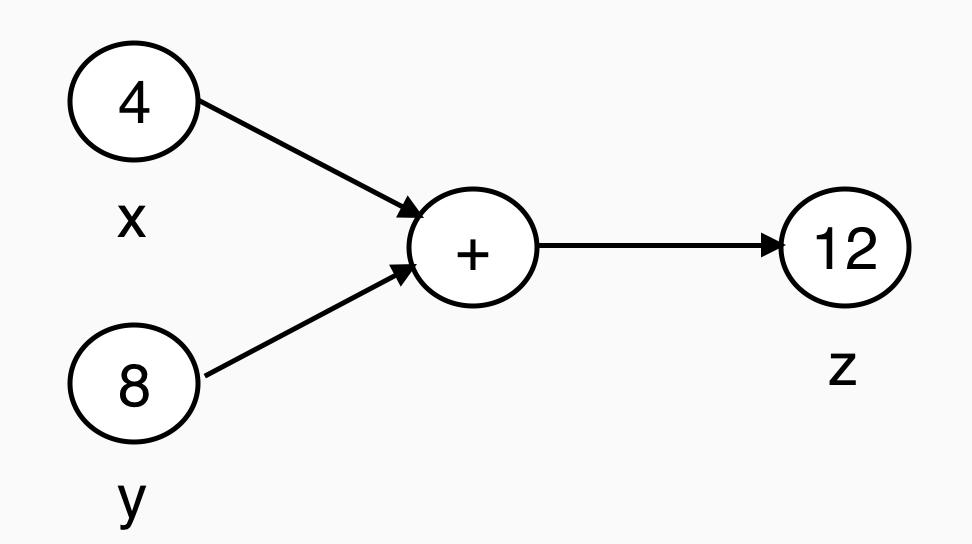
\includegraphics[scale=0.6]{dipendenza_programmazione_reattiva}
		\caption[Programmazione reattiva]{Rappresentazione della dipendenza delle variabili dell'esempio.}
		\label{figura:dipendenza_programmazione_reattiva}
	\end{center}
\end{figure}

Dal punto di vista dello sviluppo, questo paradigma offre un importante vantaggio, in quanto il programmatore deve focalizzare la sua attenzione sul \textit{che cosa deve fare} l'applicazione e può delegare la gestione al linguaggio su \textit{quando deve essere fatto}. In questo modo, al verificarsi di un evento, i cambiamenti vengono propagati attraverso la rete delle \textbf{dipendenze computazionali} dal sottostante modello di esecuzione. Per mostrare concretamente i vantaggi della programmazione reattiva, si procede con l'esposizione di un esempio:
\begin{center}
	\begin{lstlisting}
			x = 4;
			y = 8;
			z = x + y;
	\end{lstlisting}
\end{center}
La redazione di questo semplice codice con un linguaggio imperativo fa si che il risultato di \verb|z| sia 12 e che tale risultato non verrà modificato fino a quando non verrà assegnato esplicitamente un nuovo valore a tale variabile. In altri termini, \verb|z| rappresenterà sempre la somma dei due valori iniziali. L'assegnamento di nuovi valori alle variabili iniziali non influenzeranno il risultato contenuto in \verb|z|. L'esecuzione di questo codice, scritto con un linguaggio che supporta la programmazione reattiva, mantiene aggiornato il valore di \verb|z| ogni volta che almeno uno dei due addendi viene modificato: alla modifica di una delle due variabili, durante l'esecuzione del codice, viene automaticamente aggiornato il contenuto della variabile \verb|z|. Nel contesto della programmazione reattiva, la variabile \verb|z| è definita come \textit{dipendente} dalle variabili \verb|x| e \verb|y|. È possibile rappresentare graficamente la relazione di dipendenza tra le variabili del codice di esempio (Figura 4.1) \cite{reactive_programming_wikipedia}.

Il concetto di dipendenza viene realizzato attraverso l'implementazione di \textit{ascoltatori}, che riescono ad intercettare i cambiamenti delle variabili da cui essi dipendono.

\subsection{Vantaggi e svantaggi della programmazione reattiva}
Il principale vantaggio che si può ottenere dalla programmazione reattiva è la facilità di sviluppo di un'applicazione, pur mantenendo distinta la \textit{user interface} (\textit{UI}) dalla \textit{business logic}. È possibile generare del codice più compatto ed evitare di scrivere nel medesimo modulo o file sia codice per la UI e che codice per la business logic.

Tuttavia non è sempre vantaggioso l'utilizzo di questo paradigma, in quanto spesso rende complicata la leggibilità del codice. In particolare, segmentando l'interfaccia grafica in piccoli componenti, è possibile che per ogni componente debba essere associato un modulo della business logic. Pertanto, diversamente da altri linguaggi che non adottano la programmazione reattiva, la comprensione del codice non risulta essere naturale.

\section{Compilazione ed esecuzione}
\subsection{Criteri per la classificazione dei linguaggi di programmazione}
I linguaggi di programmazione possono essere classificati secondo diversi criteri, come i vari paradigmi che supportano o in base al livello a cui operano (si parla di linguaggio di \textit{alto livello} o di \textit{basso livello}). Un'altra classificazione può essere fatta suddividendo i linguaggi in \textit{linguaggi compilati} o \textit{linguaggi interpretati}.

Il sorgente di un programma scritto in un \textbf{linguaggio compilato} viene \textit{tradotto} in un programma equivalente, scritto solitamente in un linguaggio di basso livello. Questo linguaggio di basso livello è comprensibile ad una certa \textit{macchina} (macchina astratta o hardware), ovvero, all'ambiente in cui verrà eseguito il programma compilato. Oltre alle librerie e ad altri componenti esterni necessari per il funzionamento, un programma compilato non ha la necessità di utilizzare un secondo programma (l'\textit{interprete}) per poter essere eseguito. Infatti, l'assenza di un interprete per questa tipologia di linguaggi implica un minor utilizzo della memoria centrale e un minor tempo di esecuzione del codice. Tuttavia, questo fattore non è l'unico a determinare un minor tempo di esecuzione, in quanto dipende anche dalle caratteristiche della macchina su cui il programma compilato viene eseguito. Aspetto che lo differenzia dai linguaggi interpretati è l'assenza della presenza simultanea sia del compilatore che del sorgente, al momento dell'esecuzione del codice. Nei linguaggi compilati la fase di \textit{debugging} risulta essere più efficace, in quanto a tempo di compilazione possono essere scoperti degli errori sui tipi delle variabili. D'altro canto, questa restrizione può portare al negare la compilazione di programmi il cui codice è lecito durante l'esecuzione, ma che non soddisfa i controlli statici eseguiti a tempo di compilazione. I linguaggi compilati, grazie a tutti i vantaggi che offrono, vengono ampiamente utilizzati in ambiti in cui la velocità di esecuzione del codice è di fondamentale importanza, dove le risorse hardware devono essere sfruttate appieno o tali risorse sono presenti limitatamente (principalmente per sistemi e dispositivi IoT ed applicazioni real-time). In queste situazioni si preferisce avere un maggior controllo delle risorse per sfruttarle nel modo più efficace ed   efficiente possibile, a scapito di implementare con facilità il codice che dovrà essere eseguito.

Nei \textbf{linguaggi interpretati} si utilizza l'\textit{interprete}, un programma necessario per l'esecuzione del codice. L'interprete rappresenta il luogo del controllo dell'esecuzione del codice, in quanto esso riceve in input il programma da eseguire e i dati da utilizzare e passo passo traduce in linguaggio macchina ogni singola istruzione sul momento. Questo funzionamento implica che il codice da eseguire e l'interprete debbano essere necessariamente presenti al momento dell'esecuzione del programma. La presenza simultanea dell'interprete e del programma comporta ad una minore efficienza a tempo di esecuzione: un programma interpretato richiede più memoria centrale ed è meno veloce a causa dell'\textit{overhead} introdotto dall'interprete stesso. I linguaggi interpretati risultano essere più flessibili rispetto ai linguaggi compilati, in quanto tutti i controlli sui tipi (ed altri controlli) vengono effettuati al momento dell'esecuzione del codice. La fase di debugging risulta essere meno efficace in quanto è necessario eseguire il codice per scoprire eventuali bug presenti nel programma. Un notevole vantaggio che i linguaggi interpretati offrono è l'alta portabilità dei programmi, aspetto che non è possibile implementare per i linguaggi compilati in quanto il \textit{codice oggetto}, generato dal compilatore, dipende strettamente dalla macchina in cui il programma è stato compilato.

I \textbf{linguaggi semi-interpretati} o \textbf{multipiattaforma} sono dei linguaggi che cercano di unire i vantaggi sia dei linguaggi compilati che dei linguaggi interpretati. Il linguaggio che rappresenta maggiormente questa categoria è Java. I programmi scritti in Java vengono compilati in una prima fase per generare il \textit{bytecode}, un programma equivalente a quello sorgente, scritto in istruzioni macchina per una particolare \textit{macchina virtuale}: la \textit{Java Virtual Machine}. Il bytecode viene interpretato dalla JVM, la quale esegue il programma sulla macchina fisica in cui si trova. Questo livello di astrazione permette agli sviluppatori di realizzare applicazioni che siano totalmente indipendenti dall'hardware su cui verranno eseguite, ovvero, permette di avere la \textit{portabilità} delle applicazioni. Per ogni sistema operativo viene realizzata una JVM e tutte quante devono comportarsi in modo uguale. Così facendo ogni programma scritto in Java è eseguibile su ogni sistema operativo che ha una JVM. Lo slogan che esprime al meglio il concetto che sta alla base di Java è: "\textit{Write Once, Run Everywhere}". In termini di prestazioni, i programmi Java sono meno efficienti dei programmi scritti in un linguaggio compilato. Questo è dovuto al fatto che vi è una fase di compilazione del programma Java e una fase di interpretazione del bytecode. Tuttavia, la portabilità dei programmi è una caratteristica peculiare del linguaggio e risulta essere molto utile nello sviluppo delle applicazioni.

\subsection{Tipizzazione}
I linguaggi di programmazione possono essere classificati secondo un altro criterio, ovvero, in base alla loro \textit{tipizzazione}. I linguaggi possono implementare una:
\begin{enumerate}
	\item \textbf{Tipizzazione statica}: a tempo di compilazione, vengono eseguiti i controlli sull'uso corretto dei valori rispetto al loro tipo;
	\item \textbf{Tipizzazione dinamica}: i controlli sull'uso corretto dei tipi vengono fatti a tempo di esecuzione del codice.
\end{enumerate}

Non vi è una suddivisione netta tra i due insiemi: i linguaggi che implementano una tipizzazione statica eseguono comunque dei controlli a tempo di esecuzione del codice. Ad esempio, il controllo sulla dimensione di un vettore è un controllo che deve essere necessariamente fatto a tempo di esecuzione perché tale controllo non può essere effettuato in alcun modo a tempo di compilazione.

II vantaggio principale di una tipizzazione statica è la possibilità di rilevare gli errori a tempo di compilazione, prima ancora che il codice venga eseguito. Tuttavia questi linguaggi risultano essere meno flessibili rispetto ai linguaggi che adottano una tipizzazione dinamica. D'altronde, con la tipizzazione dinamica è necessario eseguire il programma per trovare eventuali errori di tipo.

Dart è considerato un linguaggio \textbf{\textit{type safe}} \cite{tipizzazione}, ovvero, garantisce l'esecuzione di controlli esaustivi sull'uso corretto dei valori rispetto al loro tipo, non solo a tempo di compilazione. La combinazione di queste due tipizzazioni fornisce una maggiore solidità al codice. Avendo una tipizzazione sia statica che dinamica, il linguaggio permette due tipologie di compilazione: \textbf{AOT} (\textbf{Ahead Of Time}) e \textbf{JIT} (\textbf{Just In Time}).

\subsection{Compilazione ed esecuzione del codice}
\subsubsection{Ahead Of Time (AOT)}
La \textbf{compilazione anticipata} consiste nel compilare un programma scritto in un linguaggio di alto livello in un codice macchina nativo, in modo che il file binario risultante possa essere eseguito nativamente. Di conseguenza, il risultato della compilazione è dipendente dal sistema su cui è stata effettuata la compilazione \cite{aot}. Eseguendo una compilazione anticipata, è possibile produrre del codice ottimizzato per la macchina, analogamente ad un normale compilatore nativo. La differenza è che la compilazione anticipata trasforma il \textit{bytecode} (codice intermedio \cite{codice_intermedio}) di una macchina virtuale esistente in codice macchina. In particolare, la compilazione anticipata permette di compilare il codice intermedio nel codice macchina prima che il codice stesso venga eseguito. In questo modo è possibile limitare l'ambiente di \textit{runtime}, risparmiando memoria, spazio su disco e durata della batteria. Per questo motivo, può essere utile per realizzare applicazioni per dispositivi mobili o per dispositivi che hanno uno spazio di memoria limitato e devono mantenere dei bassi consumi energetici.

In generale, i linguaggi statici sono gli unici linguaggi a poter supportare questa tipologia di compilazione. Il motivo è che i linguaggi macchina in genere devono conoscere il tipo delle variabili, pertanto nei linguaggi dinamici, dove il tipo non viene determinato in anticipo, questo controllo risulta essere inapplicabile. I linguaggi dinamici infatti sono in genere interpretati o compilati \textit{Just-In-Time}.

Utilizzare la compilazione anticipata durante la realizzazione del software causa dei \textit{cicli di sviluppo} più lenti. Per ciclo di sviluppo si intende il tempo che intercorre dal momento in cui viene apportata una modifica al codice di un programma e la possibilità di eseguire il programma per poter vedere il risultato, dopo tale modifica. Tuttavia questo approccio alla compilazione comporta che i programmi possono essere eseguiti in modo più prevedibile e senza la necessità di dover impiegare del tempo in fase di esecuzione del programma per l'analisi e la compilazione. Di conseguenza, grazie alla compilazione, i programmi possono essere avviati più rapidamente nella fase iniziale. 

\subsubsection{Just In Time (JIT)}
Quando la fase di compilazione viene svolta a tempo di esecuzione del codice, si sta parlando di compilazione \textbf{Just-In-Time} \cite{jit}. Nella maggior parte dei casi, si tratta di dover compilare a \textit{runtime} del codice sorgente o del bytecode in codice macchina, che viene quindi eseguito direttamente.

La compilazione JIT è una combinazione dell'approccio AOT e dell'approccio dell'interpretazione.  Si cerca di combinare la velocità del codice compilato con la flessibilità dell'interpretazione. Tuttavia questo comporta l'introduzione sia dell'\textit{overhead} di un interprete e dell'overhead della compilazione. La compilazione JIT è una forma di compilazione dinamica e consente l'attuazione di un'ottimizzazione adattiva come la \textit{ricompilazione} dinamica. La compilazione JIT è particolarmente adatta per linguaggi di programmazione dinamici, in quanto il sistema di runtime può ritardare la gestione dei tipi di dato.

Contrariamente alla compilazione anticipata, la compilazione JIT fornisce dei cicli di sviluppo molto più veloci, ma può comportare ad un'esecuzione più lenta. In particolare, i compilatori JIT hanno tempi di avvio più lenti, perché quando il programma viene mandato in esecuzione, è necessario effettuare la fase di compilazione del programma prima che il codice possa essere eseguito.

\subsection{Compilatori ed interpreti}
Potendo utilizzare Dart per la realizzazione di applicazioni che potranno essere eseguite su dispositivi di natura diversa (mobile, desktop, Web), è necessario che il linguaggio sia fornito di un compilatore sufficientemente flessibile \cite{compilazione_dart}. Infatti, i compilatori disponibili sono:
\begin{enumerate}
	\item \textbf{Dart Native}: per eseguire applicazioni su device come smartphone, desktop e per applicazioni lato server. Dart Native include sia una macchina virtuale (Dart VM) con compilazione JIT (just-in-time), sia un compilatore AOT per la produzione di codice macchina;
	\item \textbf{Dart Web}:  per eseguire il codice Dart su piattaforme Web basate su JavaScript. Dart Web include sia un compilatore dei tempi di sviluppo (\verb|dartdevc|) che un compilatore dei tempi di produzione (\verb|dart2js|). Con Dart Web, il codice Dart viene compilato in codice JavaScript, che a sua volta viene eseguito in un browser. In particolare:
	\begin{enumerate}
		\item \verb|dartdevc|: è un compilatore Dart-to-JavaScript ottimizzato. Invece di utilizzare direttamente \verb|dartdevc|, lo si utilizza con \verb|webdev|, uno strumento che supporta le attività principali dello sviluppatore come l'esecuzione e il debug \cite{dartdevc}.
		\item \verb|dart2js|: è un tool che compila il codice Dart in JavaScript velocemente e in maniera compatta. Utilizza delle tecniche per l'eliminazione del codice che non viene mai chiamato durante l'esecuzione (\textit{dead-code}).
	\end{enumerate}
\end{enumerate}

\subsection{DartVM}
La \textbf{Dart Virtual Machine} non è propriamente una macchina virtuale come la \textit{JVM}. La DartVM fornisce un ambiente di esecuzione e un insieme di componenti per l'esecuzione nativa di un linguaggio di alto livello, in questo caso Dart. Questo non implica che il codice Dart possa essere \textit{sempre} interpretato o compilato \textit{Just-In-Time} quando viene eseguito dalla DartVM. Infatti, DartVM offre diversi modi per interpretare il codice, in quanto la macchina virtuale può eseguire il codice utilizzando JIT o delle istantanee AOT. La scelta dipende principalmente da come e quando la macchina virtuale converte il codice sorgente Dart in codice eseguibile. Indipendentemente dall'opzione scelta, l'ambiente di runtime che facilita l'esecuzione rimane lo stesso.

Qualsiasi codice Dart, all'interno della macchina virtuale, è in esecuzione all'interno di un \textbf{Isolate}, ovvero uno spazio con una propria memoria e con un proprio thread di controllo. Possono esserci molti \textit{Isolate} che eseguono del codice Dart contemporaneamente, ma non possono condividere direttamente nessuno stato. Vari \textit{Isolate} possono comunicare solo tramite messaggi che passano attraverso determinate porte.

\section{Principali caratteristiche}
In questa sezione si va ad introdurre ed elencare alcuni dei costrutti fondamentali del linguaggio, che verranno successivamente utilizzati per la realizzazione del progetto.

\subsection{Isolate}
Nonostante Dart sia un linguaggio a singolo thread, offre il supporto a \verb|Future|, \verb|Stream|, lavoro in background ed altri meccanismi che permettono di scrivere codice in modo moderno, asincrono e reattivo \cite{isolate_event_loop}.

Un \verb|Isolate| è il luogo in cui viene eseguito tutto il codice Dart. È come un piccolo spazio sulla macchina con la sua zona di memoria privata ed un singolo thread che esegue un loop di eventi. Nella propria zona di memoria, nessun \verb|Isolate| è autorizzato ad accedervi, nemmeno l'\verb|Isolate| principale (che è il genitore). Da qui il nome \verb|Isolate| per enfatizzare che questi spazi di memoria sono completamente isolati l'uno dall'altro. L'unica modalità di comunicazione concessa tra \verb|Isolate| è tramite lo \textit{scambio di messaggi} tra l'uno e l'altro.

Solitamente, le applicazioni realizzare in Dart eseguono il loro codice in un singolo \verb|Isolate|, ovvero, quello principale. Se necessario, è possibile creare altri \verb|Isolate|: in particolare, quando devono essere eseguite delle elaborazioni pesanti e complesse che possono far degradare le prestazioni della UI, è possibile creare degli \verb|Isolate| separati tramite il metodo \verb|Isolate.spawn()| (nel caso di Flutter si potrà utilizzare il metodo \verb|compute()|). Così facendo, si lascia l'\verb|Isolate| principale libero e la parte più laboriosa del codice avviene in un \verb|Isolate| secondario.

\subsection{Event Loop}
\label{Event Loop}
\begin{figure}
	\begin{center}
		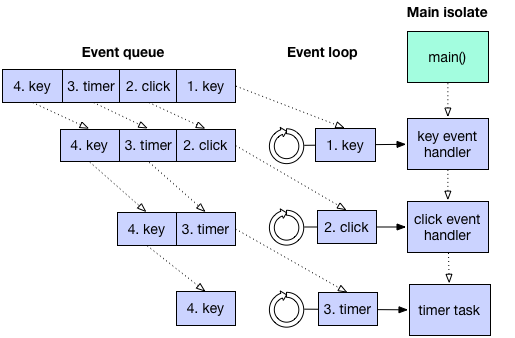
\includegraphics[scale=0.6]{event_loop}
		\caption[Event loop]{Illustrazione del funzionamento dell'\textit{event loop} \cite{event_loop}.}
		\label{figura:event_loop}
	\end{center}
\end{figure}

Un \textbf{event loop} \cite{isolate_event_loop_youtube} è una architettura asincrona che permette di inserire gli eventi generati in una coda e di gestirli uno alla volta estraendoli dalla coda ed eseguendo il rispettivo \textit{handler}. In particolare, viene preso l'evento più vecchio presente nella coda, viene eseguito il suo codice e torna ad estrarre un altro evento dalla coda, fino a quando la coda non è vuota. Questa architettura è stata pensata in quanto dal momento in cui viene avviata un'applicazione fino al momento in cui viene deallocata dalla memoria, l'applicazione non può prevedere quando dovranno essere elaborate delle operazioni di I/O, gestire il download di un file, gestire la UI ed altro ancora. Per di più, tutte queste operazioni devono essere gestite in un singolo thread che non si deve mai bloccare. Per questo motivo viene impiegato l'event loop. Ogni qualvolta si verifica un'interruzione, che può essere invocata ad esempio dall’interazione con l’utente o dalla risposta di una socket, l’event loop continua ad elaborare gli eventi fino a quando la coda non termina. In quel caso, il sistema attende la notifica di nuovi eventi. 

Tutte le API di alto livello e le funzionalità del linguaggio Dart per la programmazione asincrona, \verb|Future|, \verb|Stream|, \verb|async| e \verb|await| sono tutte basate sull'\textit{event loop}. In particolare, le API sono solo dei modi per notificare all'\textit{event loop} che è pronto del codice da eseguire. Gli \verb|Stream|, i \verb|Future| e \verb|async| e \verb|await| rappresentano le colonne portanti della programmazione asincrona in Dart.

\subsection{Future}
La problematica che può verificarsi durante l'esecuzione del codice nell'utilizzare un modello a singolo thread, è la possibilità di elaborare del \textit{codice bloccante}, il quale causerebbe il blocco il meccanismo dell'event loop. La programmazione asincrona viene utilizzata per risolvere questa problematica. Il tipo di dato \verb|Future<T>| è un’operazione asincrona che produce un risultato di tipo \verb|T| \cite{future_youtube}. Quando viene chiamato un metodo che restituisce un \verb|Future| succede che:
\begin{enumerate}
	\item Il metodo accoda le operazioni da eseguire;
	\item Al termine delle operazioni, il \verb|Future| viene completato con il risultato o con un
errore.
\end{enumerate}
Per poter utilizzare il risultato ottenuto da un metodo che restituisce un \verb|Future<T>|, vengono utilizzate delle \textbf{callback}.

Se il metodo non deve restituire alcun tipo di risultato allora il tipo di ritorno della funzione sarà \verb|Future<void>|.

\subsection{Async e await}
Nei linguaggi che supportano la programmazione asincrona, come ad esempio JavaScript, nella sintassi del linguaggio sono presenti le keyword \verb|async| e \verb|await|. \verb|async| viene utilizzato nella \textit{firma} di un metodo, per indicare che verrà restituito un \verb|Future|, o in un metodo in cui all'interno del suo corpo viene chiamato un metodo che restituisce un \verb|Future|. Mentre \verb|await| viene utilizzato per indicare di attendere che il \verb|Future| possa restituire il risultato. L'uso di \verb|await| permette di avere del codice non bloccante, permettendo all'event loop di proseguire e di non rimanere in attesa che il metodo termini. Quando le operazioni sono terminate, l'event loop riprenderà l'esecuzione dell'evento del \verb|Future| che ha prodotto il risultato.

\subsection{Stream}
Gli \verb|Stream| sono sequenze di eventi asincroni, che restituiscono un evento quando questo è terminato. Ad uno stato iniziale, lo \verb|Stream| è semplicemente un oggetto che contiene degli eventi al suo interno. Uno \verb|Stream| viene elaborato mediante l'uso di \verb|await| o mediante la callback \verb|listen()|. Quest'ultima, consente ad un \textit{Listener} di ascoltare lo \verb|Stream| e di estrarre gli eventi contenuti al suo interno.

In base alle esigenze, gli \verb|Stream| si suddividono in:
\begin{enumerate}
	\item \textbf{Single subscription stream}: gli eventi all'interno allo \verb|Stream| vengono restituiti tutti e in ordine. Questo flusso però può essere ascoltato da un solo \textit{Listener} un’unica volta. Il motivo è che un ulteriore ascolto può comportare la perdita degli eventi iniziali;
	\item \textbf{Broadcast stream}: questa modalità è destinata ai singoli messaggi che possono essere gestiti uno alla volta, come ad esempio gli eventi generati dal mouse. Più \textit{Listener} possono mettersi in ascolto sul medesimo \verb|Stream| di questa categoria e ci possono essere ascolti successivi senza che questi comportino la perdita di eventi.
\end{enumerate}

Ad uno \verb|Stream| possono essere collegai più \textit{Listener}. Quando è disponibile un nuovo evento, questo verrà notificato immediatamente a tutti gli ascoltatori collegati.

\subsection{dynamic}
Come è già stato spiegato precedentemente, Dart è un linguaggio fortemente tipizzato e supporta l'\textbf{inferenza} sui tipi. Quando però non viene dichiarato esplicitamente alcun tipo, viene implicitamente utilizzato il tipo \textbf{dynamic}. In Dart, ogni cosa è un oggetto che deriva dalla classe \verb|Object|. L’uso di \textit{dynamic} può significare che:
\begin{enumerate}
	\item È necessario rappresentare un tipo di dato non rientrante tra quelli consentiti;
	\item È necessario rappresentare un tipo di dato al di fuori dell'insieme dei tipi statici;
	\item Si dichiara esplicitamente il dinamismo per quel dato a tempo di esecuzione.
\end{enumerate}

Dal punto di vista dell'implementazione, questo significa che Dart non applica il controllo sul dato quando viene utilizzato \textit{dynamic}. Ad esempio, se si dichiara un dato di tipo \verb|A| e si prova a chiamare su quel dato un metodo non presente in \verb|A|, Dart avvisa dell'errore. Se inveve il tipo è stato dichiarato con \verb|dynamic|, è possibile chiamare qualsiasi metodo, anche se questo genererà un errore a tempo di esecuzione, in quanto Dart smette di applicare a tale dato il meccanismo di controllo statico.

\subsection{Gestore dei pacchetti}
\textbf{Pub} è uno strumento per la gestione dei pacchetti per Dart \cite{pub}. È una raccolta di plugin \textit{open source} che possono essere poi inclusi ed utilizzati nelle varie applicazioni. Sono presenti pacchetti sia per Flutter ma anche per Dart Web, Linux, macOS e Windows.

\section{Familiarità della sintassi}
La sintassi del linguaggio Dart è molto simile alla sintassi dei linguaggi Java, JavaScript e di altri linguaggi. A supporto di quanto appena affermato, si illustrano alcuni pezzi di codice scritti in diversi linguaggi che implementano il medesimo codice \cite{confronto_linguaggi}:
\begin{enumerate}
\item \textbf{Dart}


\lstset{numbers=left, % vogliamo numerare le righr
  numberstyle=\tiny, % i numeri sono piccoli
  basicstyle=\ttfamily, % usiamo il carattere dattilografico
  columns=fullflexible, % niente emulazioni di allineamento
  backgroundcolor=\color{lightgray}, % colore di sfondo
  language=Java, % linguaggio usato
  }
\begin{lstlisting}
class Segment {
	int links = 4;
	toString() => "I have $links links";
}
\end{lstlisting}

\item \textbf{Kotlin}
\begin{lstlisting}
class Segment {
	var links:  Int = 4
	override fun toString() => 
		"I have $links links"
}
\end{lstlisting}

\newpage

\item \textbf{Swift}
\begin{lstlisting}
class Segment: CustomStringConvertible {
	var links:  Int = 4
	public var description: String { return
		"I have \(links) links"
	}
}
\end{lstlisting}

\item \textbf{TypeScript}
\begin{lstlisting}
class Segment {
	links: number = 4
	public toString() = () : string => { return
		'I have ${this.links} links'
	}
}
\end{lstlisting}
\end{enumerate}

\section{Confronto con JavaScript}

\subsection{Introduzione a JavaScript}
JavaScript è un linguaggio di \textit{scripting} interpretato che permette di realizzare applicazioni sia \textit{lato client} che \textit{lato server}. È il linguaggio di scripting che viene maggiormente usato nel contesto del Web. JavaScript è un linguaggio \textit{prototype-based} ed \textit{event-driven}.

Contrariamente a quanto suggerisce il nome, JavaScript non ha alcuna correlazione con il linguaggio di programmazione \textit{Java}, se non per la sintassi. Il nome è stato scelto per ragioni di marketing piuttosto che per la vicinanza dei due linguaggi.

JavaScript non produce delle applicazioni completamente \textit{stand-alone} ma necessitano di essere eseguite in un determinato ambiente. Nel caso di applicazioni lato client, queste vengono eseguiti nel \textit{browser}. I programmi lato server, come ad esempio quelli realizzati in \textit{Node.js}, vengono eseguiti grazie ad uno specifico \textit{engine}. Sia Google Chrome che Node.js utilizzano lo stesso engine: il \textit{V8} sviluppato da Google. 

L’uso principale di JavaScript è in ambito Web per la realizzazione di potenti applicazioni Web dinamiche.

\subsection{Confronto}

\subsubsection{Class-based e prototype-based}
Come prima differenza possiamo notare che Dart è un linguaggio \textit{class-based} e non \textit{prototype-based} come \textbf{JavaScript}. Quest'ultimo è un linguaggio che si basa sugli \textit{oggetti} e non prevede l’utilizzo delle \textit{classi}. Le classi sono dei costrutti utilizzati come modelli per la creazione degli oggetti. Ogni modello può contenere degli attributi e dei metodi.
\textbf{Dart}, a differenza di JavaScript, essendo un linguaggio class-based, integra il concetto di \textit{interfaccia}, di classe e di oggetti che vengono istanziati a partire da esse.

\subsubsection{Curva di apprendimento}
Supponendo di conoscere i concetti di base della programmazione, l'apprendimento di \textbf{JavaScript} risulta essere semplice. C'è un'ampia letteratura online ed offline riguardo questo linguaggio e tutte le sue peculiarità.

Sulla base delle medesime considerazioni iniziali, la curva di apprendimento di \textbf{Dart} risulta essere leggermente più alta rispetto a quella di JavaScript. La causa è dovuta alla scarsa diffusione del linguaggio e alla poca letteratura che è stata prodotta a riguardo. La documentazione più prolissa è quella fornita da Google. Le similitudini a livello sintattico con JavaScript e Java aiutano molto l'apprendimento a quei sviluppatori che provengono appunto da esperienze con tali linguaggi.

\subsubsection{Semplicità d'uso del linguaggio}
\textbf{JavaScript} è nato nel 1995 ed è conosciuto da molti programmatori. È uno dei linguaggi più diffusi ed utilizzati nel mondo. È un linguaggio maturo, stabile ed è molto facile da utilizzare. Vi sono numerosi framework e librerie scritti in questo linguaggio.

\textbf{Dart} è un linguaggio relativamente recente per la maggior parte degli sviluppatori. Sebbene Google abbia fatto molti sforzi per documentare il linguaggio, è ancora difficile per gli sviluppatori trovare delle soluzioni a dei specifici problemi.

\subsubsection{Compilazione ed interpretazione}
\textbf{Dart} è un linguaggio compilato e questo permette di trovare la gran parte degli errori di programmazione a tempo di compilazione. Essendo inoltre \textit{type safe}, è più sicuro dal punto di vista della tipizzazione rispetto a JavaScript, rendendo più semplice il debugging delle applicazioni. \textbf{JavaScript} è un linguaggio \textit{debolmente tipizzato} ed interpretato, caratteristica strutturale che degrada le prestazioni dell'applicazione. Inoltre Dart, può essere compilato AOT o JIT in base alle esigenze e ai contesti.

\subsubsection{Web e mobile}
\textbf{JavaScript} è sicuramente il linguaggio che viene per la maggior parte utilizzato durante lo sviluppo di applicazioni mobili e Web grazie a diversi framework. JavaScript è alla base di molti framework che permettono di realizzare Web app, PWA, applicazioni ibride e cross-platform.

Analogamente a JavaScript, \textbf{Dart} può essere utilizzato sia per lo sviluppo mobile che Web. Tuttavia il successo del linguaggio è dovuta al framework \textit{Flutter}. Quindi, in questo periodo, Dart viene identificato più come un linguaggio adatto per costruire applicazioni multipiattaforma che per sviluppare applicazioni per il Web.

\chapter{Flutter}
\section{Introduzione}
\textbf{Flutter} è un framework sviluppato da Google che permette di realizzare delle applicazioni compilate nativamente per dispositivi mobili, Web e desktop a partire da un \textit{singolo codice sorgente}, scritto in \textit{Dart} \cite{flutter}. L'obiettivo è consentire agli sviluppatori di offrire app ad alte prestazioni naturali su piattaforme diverse.

\section{Struttura del framework}
\begin{figure}
	\begin{center}
		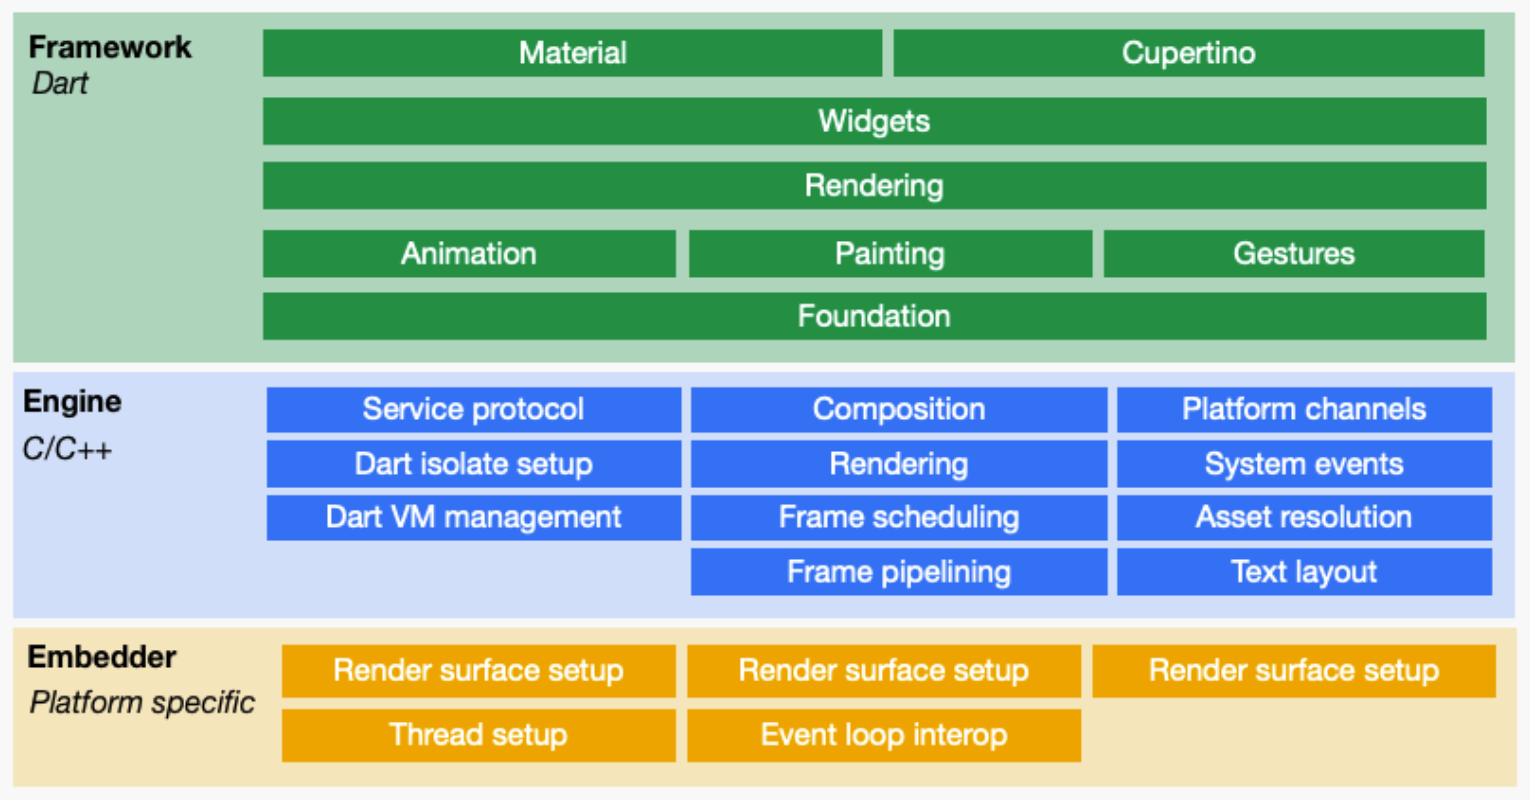
\includegraphics[scale=0.5]{architettura_framework_flutter}
		\caption[Architettura del framework Flutter]{Architettura del framework \cite{flutter_technical_overview}.}
		\label{figura:architettura_framework_flutter}
	\end{center}
\end{figure}

Il framework è strutturato a \textit{strati} con l'obiettivo di poter realizzare di più, scrivendo meno codice. È stato pensato per facilitare la stesura e la leggibilità del codice. 

Flutter si divide in:
\begin{enumerate}
	\item \textbf{Framework}: è lo strato superficiale realizzato in Dart. Vengono messe a disposizione librerie ed astrazioni necessarie per lo sviluppo dell'applicazione. In particolare è possibile notare il livello dedicato ai \textbf{Widget}, uno dei più importanti durante lo sviluppo. Sulla base di questo \textit{layer} è possibile definire altri due livelli: \textit{Material} e \textit{Cupertino}. Questi due strati implementano rispettivamente i componenti grafici secondo lo stile Android e iOS. È lo strato che viene per la maggior parte utilizzato dai programmatori durante lo sviluppo dell'applicazione. Gli sviluppatori possono creare dei nuovi componenti sulla base di quelli già forniti da Flutter o creare dei nuovi componenti ad-hoc;	
	\item \textbf{Engine}: realizzato in C++, permette di rendere le applicazioni prestanti ed efficienti. L'\textit{engine} include molti componenti di basso livello, fondamentali per il funzionamento del framework e per le sue operazioni di base. Tra questi troviamo il motore grafico \textit{Skia};
	\item \textbf{Embedder}: è il livello più basso dell’architettura e rappresenta il cuore dell'engine di Flutter. In questo strato vengono definiti gli \textit{embedder} specifici per le piattaforme, che hanno il compito di legare tra loro il rendering ai componenti della schermata nativa, alla gestione degli eventi di input e molto altro. Per implementare queste funzionalità, gli embedder interagiscono con l'engine (lo strato superiore) tramite delle API scritte in C/C++ di basso livello. Queste API non sono accessibili al programmatore, ma possono essere usate soltanto internamente da Flutter. Un altro componente importante di questo strato è la \textbf{shell} che ospita la \textit{macchina virtuale} di Dart. La shell è specifica per ogni piattaforma e offre un accesso alle API native della piattaforma in questione. Le shell implementano del codice specifico per permettere la gestione degli eventi del ciclo di vita dell’app, in base al sistema operativo di interesse.
\end{enumerate}

\subsection{Skia}
\textit{Skia} \cite{skia} è un software che permette di effettuare il \textit{rendering} dell'interfaccia grafica. Questa libreria è scritta in C++ e fornisce delle API comuni che funzionano su diverse piattaforme hardware e software (è utilizzata come motore grafico anche per \textit{Google Chrome}).

\section{Widget}
\textit{"Everything is a widget"} è il motto che più rappresenta Flutter \cite{flutter_technical_overview}.
I \textbf{Widget} sono i mattoni fondamentali dell'interfaccia utente dell'applicazione. I Widget sono tutti quegli oggetti che vengono visualizzati a schermo, con cui l'utente può interagire. I Widget, una volta dichiarati, sono \textit{immutabili}. Altri framework separano i concetti di viste, controller di visualizzazione, layout ed altre proprietà. Flutter invece raggruppa tutti questi concetti in un'unica rappresentazione, infatti, un Widget può definire:
\begin{enumerate}
	\item Una caratteristica del \textit{layout} (ad esempio, il \textit{padding});
	\item Un elemento \textit{stilistico} (ad esempio, il \textit{colore});
	\item Un elemento che va a costituire la \textit{struttura} dell'interfaccia grafica (ad esempio, un \textit{bottone}).
\end{enumerate}

Tutti i Widget che vengono utilizzati per la realizzazione della UI costituiscono una gerarchia basata sulla \textbf{composizione}. Ogni Widget eredita le proprietà dell'oggetto genitore, non esiste un Widget che sia separato da questa gerarchia. Essendo i Widget immutabili, vi è uno specifico meccanismo per gestire gli eventi. Quando l'interfaccia grafica deve essere aggiornata a seguito di un'interazione con l'applicazione, il framework viene informato di \textit{sostituire} un Widget della gerarchia (\textbf{Widget tree}) con un nuovo Widget. Il nuovo Widget può essere lo stesso di quello precedente ma con un nuovo contenuto oppure può essere un Widget differente. Quindi il framework opera un confronto tra il vecchio ed il nuovo Widget: se nota delle differenze tra i due, allora imposta il nuovo Widget, altrimenti lascia il Widget così com'è. Così facendo, si prevengono eventuali \textit{reload} inutili della UI, aggiornando la UI soltanto quando è necessario.

La composizione dei Widget è molto \textbf{flessibile}: c'è molta libertà nel comporre i vari Widget per creare degli elementi grafici \textit{personalizzati} e \textit{riusabili} in parti differenti dell'applicazione.

È rilevante precisare che il team di sviluppo di Flutter ha voluto realizzare un software differente dagli altri framework cross-platform presenti nel mercato: con Flutter è possibile personalizzare il \textbf{singolo pixel} dell'applicazione. Ai programmatori e ai designer è concessa la piena libertà nella personalizzazione della UI. Tale caratteristica permette a questo framework di differenziarsi da tutti gli altri. In particolare, diversamente da Flutter, \textit{React Native} (il principale competitor sviluppato da \textit{Facebook}) utilizza gli elementi grafici nativi che offre il sistema operativo. Ovvero, il team di React Native ha sviluppato delle API per interagire con tali componenti. Invece, nel caso di Flutter, tutti i componenti grafici sono stati completamente ridisegnati, appunto intervenendo su ogni singolo pixel. Il vantaggio di React Native è che se il sistema operativo apporta una modifica ad un componente grafico, il framework non deve essere aggiornato. Nel caso di Flutter, il team di sviluppo invece deve ridisegnare il componente e pubblicare un aggiornamento del framework. Tuttavia, Flutter lascia un'ampia libertà e flessibilità nella realizzazione degli elementi grafici, mentre React Native risulta essere più limitato da questo punto di vista, oltre ad avere la necessità di un \textit{bridge} per interagire con i componenti grafici, causando l'introduzione di \textit{overhead}.

\subsection{Classificazione dei Widget}
I Widget possono essere classificati in due categorie: possono essere \textbf{Stateful} o \textbf{Stateless}. Questa suddivisione nasce per motivi di efficienza. Come è stato accennato precedentemente, sulla base di un evento, il framework valuta se sostituire o meno un Widget. Tuttavia nell'interfaccia grafica è possibile trovare degli elementi che non vengono mai modificati durante tutto il ciclo di vita dell'applicazione: questi elementi possono essere bottoni, icone, testi ed altro ancora. Pertanto, questi Widget possono essere dichiarati \verb|Stateless|, ovvero, non necessitano di possedere uno \textbf{stato} che può cambiare nel tempo. Quindi queste tipologie di Widget, una volta \textit{renderizzate} dal framework, non vengono più aggiornate, ottenendo così delle performance migliori. I Widget vengono dichiarati \verb|Stateful| quando l'utente può interagire con loro, cambiando il loro \textit{stato}. Quando lo stato cambia, il framework si occupa di apportare le dovute modifiche, che possono essere, ad esempio, l'aggiornamento di un componente o l'aggiornamento di una variabile interna alla classe. Lo stato di un Widget è memorizzato in un oggetto di tipo \verb|State<T>|, in modo da mantenere separato lo stato del Widget dalla sua rappresentazione grafica. Quando lo stato del Widget cambia, l'oggetto \verb|State<T>| chiama il metodo \verb|setState()|, eseguendo il suo contenuto. Tuttavia, l'utilizzo del metodo \verb|setState()| comporta ad introdurre della business logic nella parte dedicata alla realizzazione dell'interfaccia grafica. Pertanto, per ovviare a questa problematica, viene sfruttata la \textit{programmazione reattiva}, presentata nel capitolo relativo all'introduzione al linguaggio Dart.

Di seguito, si illustra qual è la struttura di base per creare un \verb|Stateful| Widget e un \verb|Stateless| Widget:
\begin{enumerate}
	\item \textbf{Stateful}:
\lstset{numbers=left, % vogliamo numerare le righr
  numberstyle=\tiny, % i numeri sono piccoli
  basicstyle=\ttfamily, % usiamo il carattere dattilografico
  columns=fullflexible, % niente emulazioni di allineamento
  backgroundcolor=\color{lightgray}, % colore di sfondo
  language=Java, % linguaggio usato
  }
\begin{lstlisting}
class MyButton extends StatefulWidget {
	@override
 	_MyButtonState createState() => _MyButtonState();
}

class _MyButtonState extends State<MyButton> {
	@override
	Widget build() {
		// Build your own Widget 
		// by composing other Widgets
		return ...;
	}
}
\end{lstlisting}
	\item \textbf{Stateless}:
\begin{lstlisting}
class MyIcon extends StatelessWidget {
	@override
	Widget build() {
		// Build your own Widget 
		// by composing other Widgets
		return ...;
	}
}
\end{lstlisting}
\end{enumerate}

\subsection{Costruzione dei Widget}
\begin{figure}
	\begin{center}
		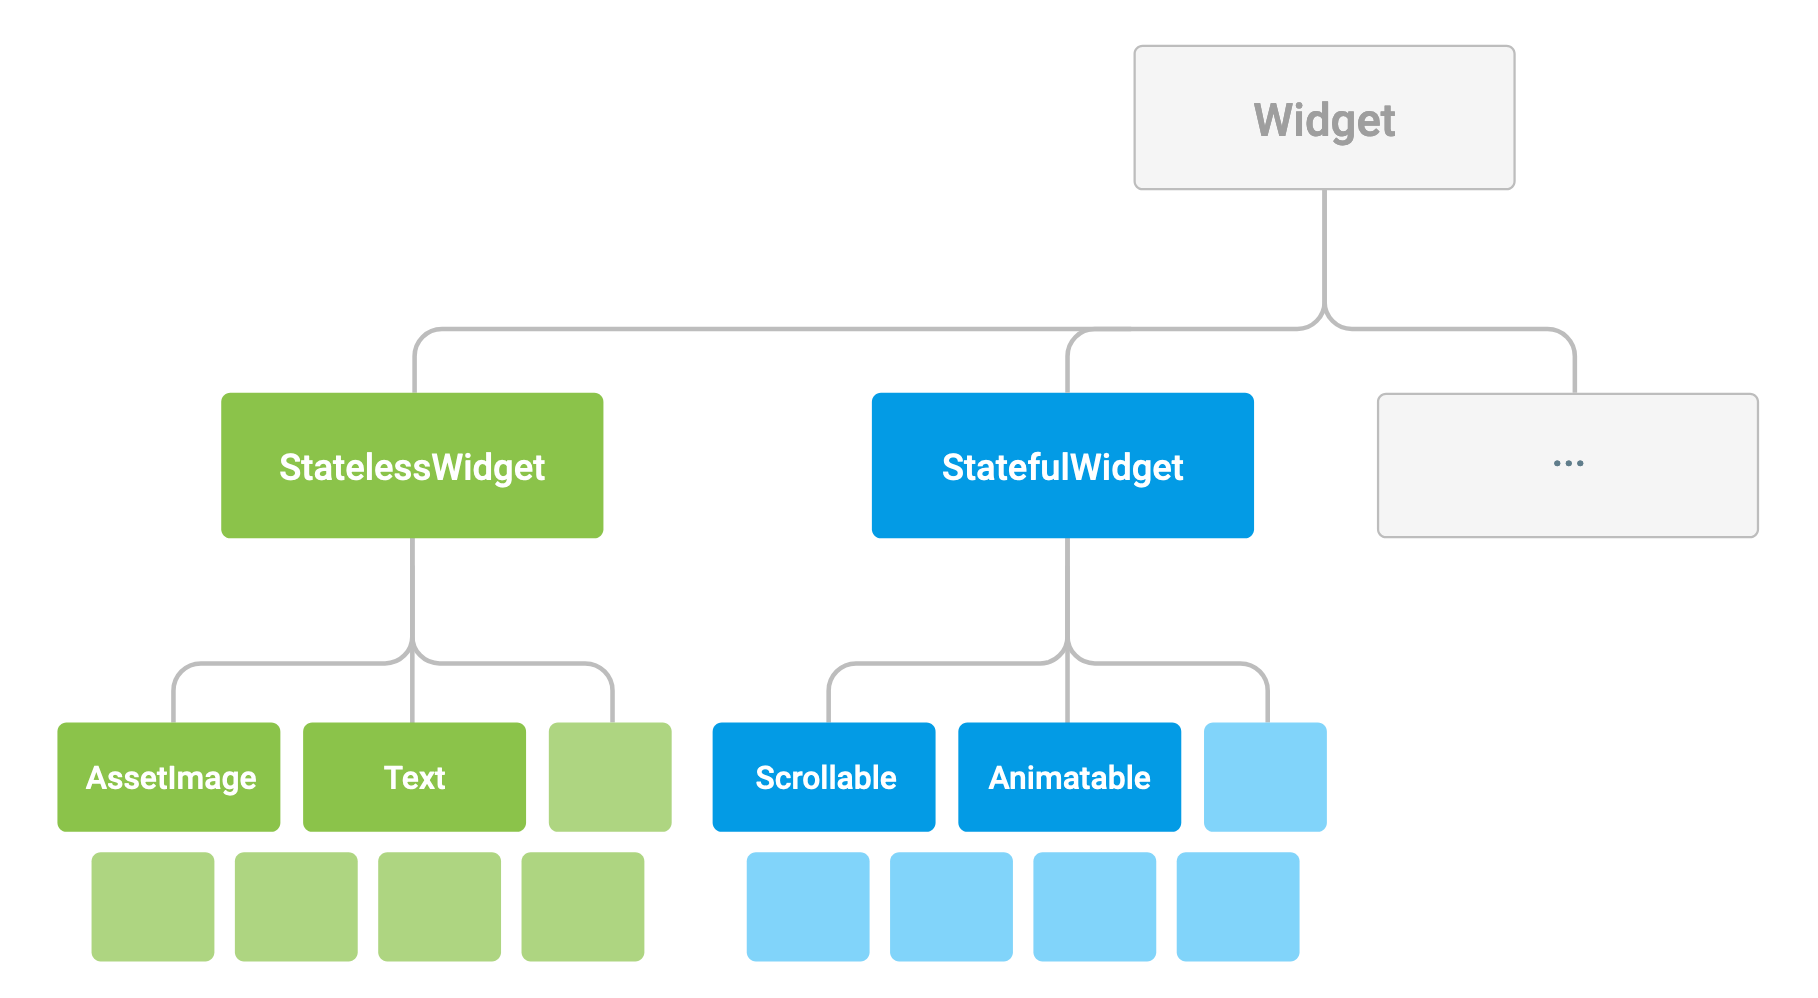
\includegraphics[scale=0.4]{stateful_stateless}
		\caption[Widget Stateful e Stateless]{Un esempio semplificato di un \textit{Widget tree} \cite{flutter_technical_overview}.}
		\label{figura:stateful_stateless}
	\end{center}
\end{figure}

Per costruire il Widget, il framework chiama il metodo \verb|build()|, presente sia nella classe \verb|Stateful| che nella classe \verb|Stateless|. Questo metodo restituisce un albero di Widget (\textit{Widget tree}). Se ci poniamo nella radice di questo albero, verrà restituito tutto l'albero dei Widget dell'applicazione; se ci poniamo in un nodo interno di questo albero, verrà restituito un sottoalbero del Widget tree. L'albero rappresenta l'interfaccia utente, realizzata per composizione con i vari Widget. A partire dalla radice, il framework chiama \textbf{ricorsivamente} il metodo \verb|build()| per ciascun Widget, fino a quando non si arriva alle foglie dell'albero, ovvero, si arriva a costruire dei Widget elementari, che non sono più costituiti da altri Widget. Un esempio semplificato di un Widget tree è illustrato nella Figura 5.2.

La creazione di un Widget dovrebbe essere \textit{priva di effetti collaterali}. A seguito di un cambiamento dello stato dell'applicazione, il framework confronta la struttura costruita precedentemente con la struttura costruita in quel preciso istante, per determinare quali modifiche devono essere apportate all'interfaccia utente. Questo confronto automatizzato risulta essere efficace, consentendo la realizzazione di applicazioni interattive e prestanti. 

L'utilizzo del metodo \verb|build()| permette di focalizzarsi sul come costruire un Widget per composizione, tralasciando la complessità dell'aggiornamento della UI da uno stato ad un altro.

\section{State Management}
L'utilizzo della programmazione reattiva porta a gestire in maniera differente i dati che devono essere comunicati tra i vari componenti. Nella comunità di Flutter, questo è un tema sempre molto discusso, da cui fuoriescono diverse soluzioni e possibili architetture per gestire in modo efficiente la \textit{gestione dello stato} (\textit{state management}). Una qualsiasi modifica, come la ricezione di un messaggio o l'interazione dell'utente con l'app, può essere intesa come una variazione dello stato dell'applicazione. Questo aspetto è di fondamentale importanza in quanto è una caratteristica intrinseca del framework: pertanto, questo tema deve essere affrontato ampiamente, andando ad analizzare la documentazione fornita dalla comunità di Flutter. Se lo \textit{state management} non viene gestito correttamente durante lo sviluppo dell'applicazione, non solo si possono ottenere delle inefficienze dal punto di vista delle prestazioni, ma anche delle vere e proprie problematiche nella comunicazione dei cambiamenti di stato, che possono causare, per esempio, la mancata ricezione di alcuni dati. Nel contesto d'uso in cui l'applicazione deve far parte, è necessario porre molta attenzione nella ricerca e nello sviluppo di un'architettura che riesca a gestire correttamente lo \textit{state management}.

Di seguito vengono elencate le diverse soluzioni ed architetture proposte fino ad ora, sia dal team di Flutter che dalla comunità.

\subsection{setState}
Questo è l'approccio di gestione dello stato più semplice presente in Flutter. Tramite la funzione \verb|setState()| è possibile indicare nel suo corpo tutte le operazioni che modificano il valore di un qualche oggetto dell'applicazione. Questo oggetto è condiviso da più Widget e pertanto la modifica di tale deve avvenire all'interno del metodo \verb|setState()| in modo da forzare il framework ad aggiornare i rispettivi Widget.

I vantaggi sono la facilità di utilizzo e la facilità di comprensione del meccanismo. Tuttavia, quando l'applicazione cresce di complessità, questo approccio risulta essere molto limitante. Gli altri svantaggi sono:
\begin{enumerate}
	\item Non è possibile gestire degli stati che devono persistere tra le sessioni;
	\item L'utilizzo di questo approccio rende il processo di manutenzione molto più laborioso e complicato in quanto lo stato viene sparso in varie zone dell'applicazione;
	\item Si inserisce nel codice dedicato all'interfaccia grafica, mescolando UI e business logic;
\end{enumerate}

Questo approccio è consigliato per la realizzazione di piccole applicazioni e che in futuro non verrano ampliate.

\subsection{InheritedWidget}
\verb|InheritedWidget| è un Widget che non mostra nulla a livello grafico ma permette di salvare dei dati al suo interno e di propagarli nel Widget tree a lui sottostante. I Widget dell'albero possono accedere ai dati del \verb|InheritedWidget| tramite il metodo \verb|InheritedWidget.of(context)|. Questo approccio è alla base del pattern Provider e viene ampiamente utilizzato anche per la creazione di molti componenti di default di Flutter.

\newpage

\subsection{Scoped Model}
Lo \verb|Scoped Model| è un approccio basato su \verb|InheritedWidget| e offre un modo, leggermente migliore, per accedere, aggiornare e mutare lo stato. Permette di passare facilmente un \verb|Model| di dati da un Widget genitore ai suoi discendenti. Inoltre, ricostruisce anche tutti i \textit{child} che utilizzano tale modello, nel momento in cui questo viene aggiornato. Così facendo, potrebbero sorgere delle problematiche relative alle prestazioni, a seconda di quanti \verb|ScopedModelDescendants| ha un modello. I \verb|ScopedModelDescendants| vengono ricostruiti ogni qual volta è presente un nuovo aggiornamento dello stato. Questo problema può essere risolto decomponendo lo \verb|ScopedModel| in più modelli, in modo da ottenere delle dipendenze più precise. 

Specificando il flag \verb|rebuildOnChange| su \verb|false|, viene risolto il problema, in quanto si va a specificare quale Widget necessita di essere ricostruito all'aggiornamento dello stato.

\subsection{Redux}
\begin{figure}
	\begin{center}
		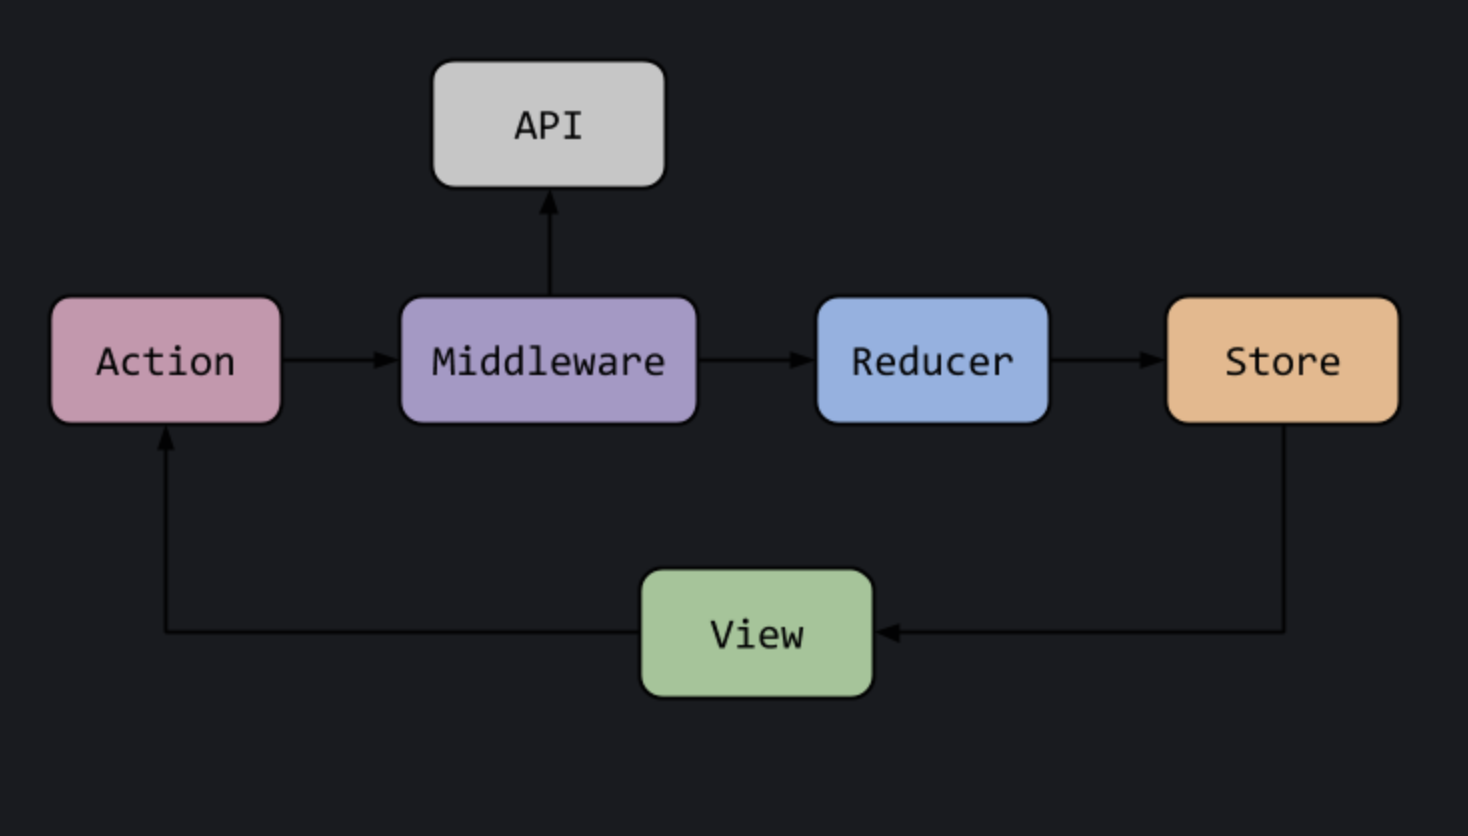
\includegraphics[scale=0.4]{redux}
		\caption[State management - Redux]{Il pattern architetturale Redux.}
		\label{figura:redux}
	\end{center}
\end{figure}

\textbf{Redux} è un'architettura nella quale è presente un unico flusso unidirezionale dei dati che semplifica lo sviluppo, la manutenzione e il test delle applicazioni \cite{redux}.

È una nota libreria JavaScript ampiamente utilizzata in React. Grazie al suo successo, è stato effettuato un \textit{porting} della libreria per Flutter.

\subsection{Provider e BLoC}
Questi due pattern architetturali verranno descritti ampiamente nel capitolo successivo, in quanto sono i due principali metodi utilizzati per la realizzazione dell'architettura complessiva dell'applicazione.

\section{Hot Reload}
Questa rappresenta una delle funzionalità più apprezzate dagli sviluppatori Flutter. Google tentò più volte di implementare \textit{Instant Run} per lo sviluppo di applicazioni per Android, ma con scarsi successi.

Nella fase di sviluppo di un'applicazione, Flutter utilizza il compilatore \textit{JIT}. L'\textit{hot reload} permette di ricaricare e di continuare l'esecuzione del codice, in pochi decimi di secondo. Lo stato dell'applicazione rimane inalterato tra un \textit{reload} e l'altro quando possibile: se avviene un aggiornamento dal punto di vista grafico, allora lo stato rimane inalterato; se invece l'aggiornamento apportato riguarda una modifica fatta a livello di business logic, allora è possibile che lo stato venga alterato. In quel caso sarà necessario ricompilare l'applicazione per ripristinare uno stato consistente. 

Questa funzionalità accelera i tempi di sviluppo dell'interfaccia grafica in quanto vengono eliminati tutti i tempi di attesa, dal momento in cui viene avviata la nuova compilazione fino al suo termine. Pur sembrando irrisori, la somma di tutti questi tempi morti comporta a risparmiare molto tempo durante l'intero processo di sviluppo e anche durante la fase di \textit{debugging} \cite{hot_reload}.

\section{Fuchsia}
\begin{figure}
	\begin{center}
		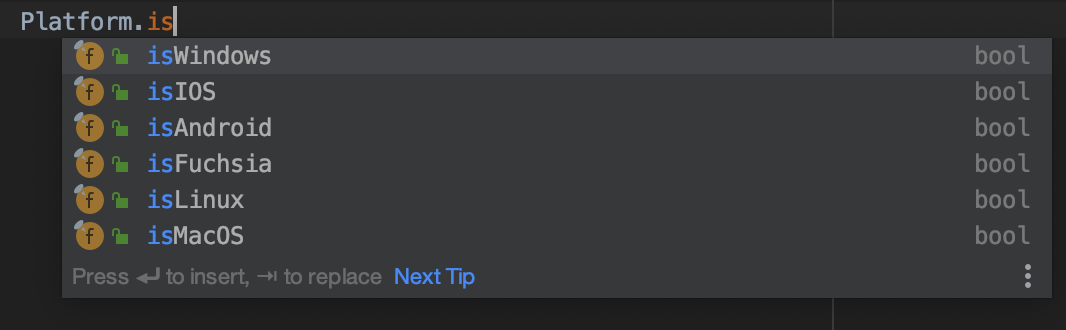
\includegraphics[scale=0.7]{fuchsia_multipiattaforma}
		\caption[Flutter - Supporto sistemi operativi]{Già da diverse verisioni dell'SDK di Flutter, sono presenti alcuni suggerimenti per il futuro supporto di Fuchsia (la versione di Flutter in questione è la \textit{1.12.13+hotfix.9} del canale stabile e la versione di Dart è la \textit{2.7.2}).}
		\label{figura:fuchsia_multipiattaforma}
	\end{center}
\end{figure}

Lo sviluppo di questo framework fa parte di un contesto molto più grande di quello attuale. Negli ultimi anni Google ha iniziato a sviluppare un nuovo sistema operativo denominato \textbf{Fuchsia} \cite{fuchsia} \cite{fuchsia_wikipedia}. A differenza dei precedenti sistemi operativi, come Android e Chrome OS, che si basano su kernel \textit{Linux}, Fuchsia si basa su un nuovo \textit{microkernel} denominato \textbf{Zircon}, derivato da \textit{Little Kernel (LK)}, progettato per funzionare su qualsiasi dispositivo. In particolare è stato progettato per funzionare su smartphone e computer moderni, con processori veloci, quantità molto alte di memoria RAM e con periferiche arbitrarie per il calcolo computazionale.

Flutter diventerà il principale framework di sviluppo per le applicazioni di Fuchsia. Per essere più precisi, l'SDK di Flutter sarà nativamente supportato dal futuro sistema operativo (si veda Figura 5.3).

Una delle proprietà più rilevanti di Fuchsia che è possibile notare è la capacità di adattare l'interfaccia grafica a seconda del dispositivo in cui viene eseguito, tutto in maniera estremamente semplice. L'obiettivo di Google è un obiettivo molto ambizioso, intrapreso recentemente da diverse aziende tecnologiche come Mircrosoft, Samsung ed Apple. In particolare:
\begin{enumerate}
	\item Microsoft ha tentato l'unificazione con la \textit{Universal Windows Platform} (UWP), progetto naufragato a causa della rimozione del supporto a \textit{Windows Mobile}. L'obiettivo era quello di realizzare applicazioni universali che potessero essere eseguite su Windows 10, Windows 10 Mobile e Xbox One;
	\item Samsung ha avviato \textit{Samsun DeX}: collegando il proprio smartphone al ad un monitor e ad una tastiera è possibile utilizzarlo tramite un'interfaccia che si adatta alle dimensioni di un monitor;
	\item Apple ha presentato \textit{Apple Catalyst}, un software che permette di creare applicazioni che possono essere eseguite sia su Mac che iPad.
\end{enumerate}

Osservando tutte queste iniziative  avviate dalle più grandi aziende tecnologiche al mondo, è facile intuire che il futuro sarà l'unificazione dei dispositivi mobili, tablet e desktop dal punto di vista delle applicazioni.

Nell'ultimo periodo, Fuchsia è stato testato su un insieme di dispositivi molto differenti tra loro: è stato testato su uno smartphone Huawei, su un Google Nest Hub \cite{fuchsia_google_nest_hub}, Chromebook ed altri.

\section{Ciclo di vita delle applicazioni}
Il \textit{ciclo di vita} di un'applicazione Flutter è leggermente differente sia dal ciclo di vita di un'app Android che iOS. Il motivo è che essendo un framework cross-platform, deve riuscire ad interagire con entrambi i sistemi operativi. Pertanto, risulta necessario avere un ciclo di vita comune a tutti i sistemi operativi. Gli eventi nel ciclo di vita di un'app in Flutter sono:
\begin{enumerate}
	\item \textbf{inactive}: l’applicazione è inattiva e non riceve input dall’utente. Questo evento funziona solo per iOS in quanto non esiste un evento corrispondente in Android;
	\item \textbf{paused}: l’applicazione non è momentaneamente visibile all’utente, non risponde ai suoi input ed è eseguita in background (corrisponde all'evento \verb|onPause()| di Android);
	\item \textbf{resumed}: l’applicazione è visibile e risponde all’input dell’utente (corrisponde all'evento \verb|onPostResume()| di Android);
	\item \textbf{suspending}: l’applicazione è momentaneamente sospesa. Equivale all'evento \verb|onStop()| di Android. Non esiste un evento corrispondente su iOS.
\end{enumerate}

Flutter non mette a disposizione molti metodi per il controllo del ciclo di vita. Il motivo è che ci sono poche argomentazioni valide per osservare il ciclo di vita dal punto di vista di Flutter e quindi tali metodi vengono nascosti allo sviluppatore. Questi metodi vengono eseguiti internamente dal framework. Nel caso fosse strettamente necessario dover osservare il ciclo di vita per poter acquisire o rilasciare delle risorse, è preferibile farlo nativamente.

\section{Pacchetti}
In precedenza è stato introdotto il \textit{Pub} di Dart, ovvero, una raccolta di pacchetti open source disponibili anche per Flutter. In un'applicazione Flutter, questi pacchetti devono essere annotati dal programmatore su un particolare file: \textbf{pubspec.yaml}. Questo file è presente in qualsiasi progetto Flutter, fin dal momento della sua creazione. In questo file sono contenute:
\begin{enumerate}
	\item Tutte le dipendenze dell'applicazione;
	\item I percorsi degli \textit{asset} (ad esempio: icone, immagini, file JSON, font);
\end{enumerate}

Per importare nel progetto un pacchetto, è sufficiente scrivere sotto la voce \verb|dependencies| il nome e la versione del pacchetto (ad esempio, \\ \verb|url_launcher: ^5.4.7|\cite{pacchetto_url_launcher}). Successivamente sarà necessario lanciare il comando \verb|flutter pub get| per poter scaricare il pacchetto desiderato. Non è necessario effettuare il download manuale, è sufficiente indicare il nome e la versione del plugin e il sistema provvederà a scaricarlo e ad integrarlo automaticamente nel progetto.

\section{Vantaggi e svantaggi di Flutter}
In conclusione ai capitoli relativi a Dart e Flutter, si elencano alcuni vantaggi e svantaggi dell'utilizzo congiunto di questo linguaggio e di questo framework, sulla base anche dell'esperienza ottenuta durante lo sviluppo del progetto.

I vantaggi di utilizzare Flutter come framework di sviluppo sono:
\begin{enumerate}
	\item \textbf{Hot Reload}: funzionalità che consente di visualizzare le modifiche apportate al codice quasi in tempo reale, senza necessità di riavviare l'applicazione. Le modifiche apportate vengono inserite nell'applicazione in esecuzione e Flutter ricostruisce automaticamente il Widget tree in modo che tali modifiche vengano visualizzate in tempo reale;
	\item \textbf{Prestazioni}: Flutter non utilizza alcun \textit{bridge} in JavaScript per visualizzare in modo reattivo l'applicazione, come nel caso di React Native. L'applicazione quindi risulterà più prestante e veloce;
	\item \textbf{Programmazione reattiva}: permette di non fare uso del metodo \\ \verb|setState()|, migliorando la \textit{riusabilità del codice}, in quanto rende possibile la separazione della business logic dall'interfaccia grafica. Inoltre, migliora le prestazioni dell’applicazione, poiché evita di ridisegnare un Widget e l’intero Widget tree ad ogni modifica apportata. Le modifiche vengono propagate mediante gli \verb|Stream|.
\end{enumerate}

Di seguito, si elencano gli svantaggi dell'utilizzo di Flutter e, più in generale per alcuni punti, dei framework cross-paltform:
\begin{enumerate}
	\item \textbf{Dart}: diversamente da altri framework che utilizzano dei linguaggi già affermati nel mondo dello sviluppo software (JavaScript nel caso di React Native e C\# nel caso di Xamarin), imparare un nuovo linguaggio comporta comunque il dover superare una certa \textit{curva di apprendimento}, seppur bassa. La curva di apprendimento è bassa ed è dovuta alla vicinanza di Dart a linguaggi come JavaScript e Java, che semplificano l'apprendimento di tale linguaggio.
	\item \textbf{Multipiattaforma}: con un accezione negativa, non è possibile sviluppare delle applicazioni che devono implementare delle funzionalità che sfruttano dei particolari servizi offerti dal sistema operativo;
	\item \textbf{Dimensioni dell'applicazione}: non possono essere create delle applicazioni di dimensioni inferiori ai 4 MB. Il motivo riguarda la natura stessa di Flutter: nel codice dell'applicazione devono essere inclusi tutti i Widget necessari, in quanto il framework non utilizza i componenti grafici offerti dal sistema operativo;
	\item \textbf{Programmazione reattiva}: non sempre è possibile utilizzare la programmazione reattiva, spesso rende difficoltosa la leggibilità del codice, specialmente se la struttura dei Widget implementati è complessa.
\end{enumerate}

\section{Confronto con React Native}

\subsection{Introduzione a React Native}
\textbf{React Native} è un framework JavaScript per lo sviluppo di applicazioni mobili che permette di effettuare il rendering nativo sia per iOS che per Android. Questo framework si basa su \textit{React}, la libreria JavaScript di Facebook per la creazione di interfacce utente Web. Il motivo di questa scelta risulta essere molto astuta: Facebook può coinvolgere gli sviluppatori, che già conoscono la versione Web, verso lo sviluppo di applicazioni multipiattaforma, senza dover far imparare  agli sviluppatori delle nuove logiche ed una nuova architettura per realizzare applicazioni mobile. Gli sviluppatori dovranno fare un minimo sforzo per capire in che modo il framework interagisce con i dispositivi.

Analogamente a \textit{React.js} (la libreria Web), le applicazioni React Native sono scritte usando una combinazione di JavaScript e XML, noto come \textit{JSX}. Quindi, il \textbf{bridge} nativo di React invoca le API di rendering native in Objective-C (per iOS) e in Java (per Android). Pertanto, l'applicazione eseguirà il rendering utilizzando i componenti grafici già presenti nel sistema operativo, senza effettuare visualizzazioni Web. React Native espone anche le interfacce JavaScript per le API della piattaforma, quindi le applicazioni React Native possono accedere a funzionalità del dispositivo come la videocamera del telefono o la posizione dell'utente.

\subsection{Confronto}

\subsubsection{Linguaggio di programmazione utilizzato}
\textbf{React Native} utilizza JavaScript per creare le applicazioni. JavaScript è un linguaggio molto popolare nello sviluppo di applicazioni Web. Con React Native, gli sviluppatori Web possono creare delle applicazioni mobili, aggiungendo poche conoscenze basilari.

\textbf{Flutter} utilizza \textit{Dart} come linguaggio per scrivere le applicazioni. È stato introdotto da Google e il suo uso è limitato a questo framework. La sintassi Dart è di facile comprensione per gli sviluppatori JavaScript o Java, in quanto supporta la maggior parte dei concetti orientati agli oggetti. Inoltre il linguaggio è provvisto di una buona documentazione.

\textit{JavaScript} è ampiamente utilizzato dalla maggior parte degli sviluppatori Web: di conseguenza è facile adottare il framework React Native. Nonostante Dart abbia delle ottima funzionalità e caratteristiche, è usato raramente ed è meno conosciuto nella comunità degli sviluppatori.

\subsubsection{Architettura}
L'architettura di \textbf{React Native} si basa fortemente sull'architettura dell'ambiente di runtime Javascript, ovvero, il \textbf{bridge}. React Native lo utilizza per comunicare con i moduli nativi del dispositivo. Questo intermediario tra l'applicazione e il dispositivo comporta ad un degrado delle prestazioni e ad una perdita di efficienza.

In \textbf{Flutter}, diversamente, tutti i componenti sono integrati nell'applicazione: questo comporta una maggiore dimensione dell'applicazione una volta che questa deve essere installata sul dispositivo. Tuttavia, permette di interagire in modo diretto con i moduli nativi, senza aver la necessità di un \textit{bridge}. In questo modo, le prestazioni di un'app realizzata con questo framework si avvicinano a quelle di un'applicazione nativa.

\subsubsection{Installazione}
Il framework \textbf{React Native} può essere installato utilizzando \textbf{Node Package Manager} (\textbf{NPM}). Per gli sviluppatori che già conoscono JavaScript, l'installazione di React Native risulta essere semplice e familiare. Questo gestore dei pacchetti può installare i pacchetti localmente o globalmente. Sta allo sviluppatore capire dove si trovano esattamente i binari.

\textbf{Flutter} può essere installato scaricando il binario, per una piattaforma specifica, da \textit{Github}.  L'installazione di Flutter richiede diversi passaggi da svolgere per poterlo integrare nel sistema. Il meccanismo usato da React Native risulta essere molto più intuitivo, semplice e diretto, senza la necessità di dover scaricare manualmente i binari.

Tuttavia entrambi mancano di un'installazione \textit{one-liner} con gestori di pacchetti nativi per un sistema operativo specifico.

\subsubsection{Setup e configurazione del progetto}
La guida relativa a \textbf{React Native} assume come base di partenza che lo sviluppatore abbia già tutte le conoscenze necessarie per lo sviluppo per iOS ed Android. Vengono fornite poche informazioni per il setup corretto dell'IDE. La documentazione passa direttamente alla fase di creazione del progetto.

La guida introduttiva per \textbf{Flutter}, invece, contiene informazioni dettagliate riguardo la configurazione dell'IDE e l'introduzione alle piattaforme iOS ed Android. Inoltre, Flutter ha uno strumento da linea di comando chiamato \verb|flutter doctor|, che può guidare gli sviluppatori attraverso l'installazione. Questo tool controlla quali pacchetti sono installati sul computer locale e quali strumenti devono essere configurati.

\subsubsection{Componenti grafici e API di sviluppo}
\textbf{React Native} di base fornisce soltanto il rendering dell'interfaccia utente e le API per accedere ai moduli del dispositivo. Per accedere alla maggior parte dei moduli, React Native deve fare affidamento su librerie di terze parti. Purtroppo, React Native dipende troppo dalle librerie di terze parti.

\textbf{Flutter} fornisce molti componenti di rendering dell'interfaccia utente, l'accesso all'API del dispositivo, una gestione dello stato (\textit{state management}) e molte librerie. Questo ricco set di componenti elimina la necessità di utilizzare librerie di terze parti. Tutto il necessario per sviluppare un'applicazione in Flutter viene fornito direttamente dal framework, una volta installato. In Flutter sono stati implementati manualmente, dal team di sviluppo, i Widget per Material e Cupertino, che consentono agli sviluppatori di eseguire facilmente il rendering dell'interfaccia sia su Android che iOS.

\subsubsection{Supporto della community}
\textbf{React Native} è stato rilasciato nel 2015 e da allora ha ottenuto molto successo. Negli anni molti sviluppatori si sono avvicinati a questo framework ed ora React Native può vantare un solido seguito di programmatori.

\textbf{Flutter} ha attirato molta attenzione dal momento in cui Google lo ha promosso nella conferenza \textit{I/O} nel 2017. La comunità Flutter sta crescendo rapidamente in questo ultimo periodo; tuttavia, gli sviluppatori non dispongono ancora di risorse sufficienti per risolvere problemi specifici.

\subsubsection{Testing}
Essendo \textbf{React Native} un framework JavaScript, Internet pullula di framework per effettuare test a livello di unità, come ad esempio \textit{Jest}. Tuttavia, quando si tratta di test a livello di integrazione o di interfaccia utente, React Native non offre alcun supporto ufficiale.

\textbf{Flutter} offre un ricco set di funzionalità per testare le applicazioni a livello di unità e di integrazione. Flutter ha un'ottima documentazione sul testing delle applicazioni, oltre ad avere un'apprezzata funzionalità per testare i Widget: è possibile eseguire dei test per l'interfaccia utente ed eseguirli alla velocità dei test unitari.

 \chapter{Sviluppo dell'applicazione}
In questo capitolo verranno trattati gli argomenti relativi alla progettazione e allo sviluppo concreto dell'applicazione. Si procederà con l'introduzione dei \textit{requisiti} che l'applicazione deve soddisfare, per poi esporre le scelte progettuali e le motivazioni che hanno portato alla realizzazione dell'architettura finale. Le varie architetture verranno introdotte prima da un punto di vista teorico, per poi affrontare una spiegazione più tecnica, strettamente legata all'effettiva implementazione.

\section{Requisiti}
L'applicazione deve essere in grado di interrogare un server tramite una \textit{socket}, la quale invierà come risposta il set di dati, rilevati dai sensori installati sulla barca. L'applicazione deve svolgere un \textit{polling} della socket, periodicamente per un tempo prefissato. Questi dati dovranno essere organizzati e visualizzati su più schermate, in modo da facilitare l'utente nel monitorare i dati di cui necessita.

Rispetto all'applicazione Android sviluppata precedentemente, si vuole ridisegnare l'interfaccia grafica in modo da rendere la visualizzazione dei dati il più efficace possibile.

Si vuole inoltre disporre di alcune funzionalità come la possibilità che l'utente possa decidere ogni quanti secondi interrogare il server e che questo non sia un parametro fisso integrato nel codice.

In conclusione, si vuole rendere l'applicazione disponibile sia per gli utenti con dispositivi Android che iOS. Pertanto la scelta di un framework cross-platform risulta essere adatta nel rispettare questa particolare richiesta.

\section{Architetture utilizzate}

\subsection{Introduzione}
L'architettura rappresenta l'elemento fondante di tutta l'applicazione. Essa permette di definire le logiche e i comportamenti che avrà l'applicazione al termine dello sviluppo e definisce anche in che modo deve avvenire la cooperazione tra i vari componenti dell'applicazione. Un altro fattore importante da tenere in considerazione è il contesto in cui l'applicazione verrà utilizzata. Quindi, è necessario quindi scegliere attentamente l'architettura corretta sulla base dei requisiti e del risultato finale che si vuole ottenere. Il processo di scelta dell'architettura richiede una certa esperienza nella programmazione, nel conoscere il framework con il quale si creerà l'applicazione ed una conoscenza delle nozioni di \textit{ingegneria del software}.

Nella scelta dell'architettura influiscono anche proprietà come le \textit{prestazioni} che si vogliono ottenere e la \textit{flessibilità} dell'architettura stessa, necessaria per poter supportare l'implementazione di nuove funzionalità in futuro.

In conclusione, la scelta dell'architettura è una fase particolarmente delicata ed importante in quanto determinerà il successo nel raggiungere i requisiti richiesti o il mancato raggiungimento di essi.

\subsection{Scelta dell'architettura}
L'architettura scelta farà un largo uso della \textit{programmazione reattiva}, caratteristica peculiare del linguaggio del framework.

Un principale svantaggio dell'utilizzo di Flutter come framework di sviluppo è il suo recente rilascio nel mercato. Essendo un framework relativamente nuovo rispetto agli altri, la comunità di Flutter ha proposto diverse architetture e pattern per implementare le applicazioni. Tuttavia, Google non ha mai fornito un supporto alla realizzazione di un qualche pattern ideale nelle sue guide relative al framework. Nella sua documentazione, il team di Flutter ha soltanto racchiuso in una pagina una serie di link alle risorse che illustrano alcuni pattern, spiegati da chi li hanno ideati. Pertanto, la ricerca e l'analisi di dell'architettura adatta è un processo più laborioso rispetto ad altri framework già affermati nel mercato.

\newpage

\subsection{Provider}
L'introduzione di questo pattern è di fondamentale importanza in quanto rappresenta il fulcro di tutto il pattern architetturale finale dell'applicazione. 

Una delle possibili definizioni per il pattern \textbf{Provider} può essere la seguente: \textit{"Il pattern Provider condivide i valori tra Widget tree e i Widget facenti parte dell'albero vengono ricostruiti in base ai cambiamenti di stato avvenuti nell'applicazione"}. Esaminando questa definizione è possibile affermare che:
\begin{enumerate}
	\item Il Provider è un Widget;
	\item Le dipendenze di un Provider sono dei Widget tree;
	\item Il Provider si occupa di aggiornare i Widget nel momento in cui rileva un cambiamento di stato;
\end{enumerate}

Da queste considerazioni, si può capire che l'aggiornamento debba avvenire in modo \textit{asincrono} e debba essere \textit{reattivo}. In particolare, i Widget che non cambiano con la generazione di un nuovo stato, non necessitano di dover rimanere in ascolto di un nuovo stato; i Widget che cambiano nel momento in cui viene rilevata una variazione dello stato dell'applicazione, devono rimanere in ascolto non appena un nuovo stato viene creato. Pertanto, in quest'ultima casistica, verranno utilizzati \verb|Future| e \verb|Stream|. 

Quando lo stato cambia, questo viene fornito al Provider piuttosto che a ciascun discendente (Widget). Per fare ciò il Provider utilizza internamente un \verb|InheritedWidget|, un oggetto che permette di propagare, in modo efficiente, i cambiamenti lungo il Widget tree. La gestione dell'aggiornamento dei Widget tree rappresenta uno dei principali problemi dello sviluppo dell'applicazione, in quanto questo fattore può essere uno dei principali responsabili del degrado delle prestazioni.

Il Provider rappresenta, sostanzialmente, un mezzo per condividere un valore per i Widget che ne necessitano. Con le successive spiegazioni, si andrà ad apprezzare la \textit{flessibilità} di questo pattern.

\subsubsection{Strutturazione del Provider}
Ricordando che questo pattern è un Widget e pertanto si inserirà nel Widget tree complessivo dell'applicazione, ogni Provider ha un \textit{figlio} (il parametro \verb|child|) che rappresenta la radice di un certo Widget tree (sottoalbero del Widget tree dell'app). Il Provider rende il valore disponibile per tutti i Widget a loro sottostanti. Ogni Widget decide individualmente se utilizzare o meno il valore ricevuto.

Non ci sono restrizioni su ciò che può essere un \textit{valore}. Può essere un \textit{servizio} (ad esempio un API), un \textit{modello} o uno \textit{stato}. Un modello potrebbe essere un oggetto che rappresenta una certa entità, come ad esempio un messaggio o un utente. Uno stato potrebbe essere il valore di un campo, la quantità di dati finora caricati o lo stato di riproduzione di un flusso di dati audiovisivo.

La scelta di non prendere i nuovi valori da delle variabili globali visibili a tutti i Widget che ne necessitano, è dovuta alla rigida gerarchia dei Widget tree, la quale impedisce che si verifichino delle \textit{dipendenze circolari}. Un'altra ragione, riguarda il passaggio di un valore attraverso più costruttori per farlo raggiungere ad uno specifico Widget dell'albero. Questa tecnica rende il codice complesso e verboso, pertanto vengono utilizzate le tecniche di \textit{dependency injection}.

Il Provider viene creato prima di istanziare tutti i Widget dipendenti che esso contiene (Figura 6.2). Costruire per primo il Provider, permette di avere già a disposizione dei valori per i Widget discendenti che \textbf{non sono ancora stati costruiti}. Quando i Widget dipendenti vengono successivamente creati, essi hanno accesso a tali valori e possono effettuare le loro modifiche grafiche in base ai valori ricevuti.

\subsubsection{Recuperare ed utilizzare i valori dal Provider}
\begin{figure}
	\begin{center}
		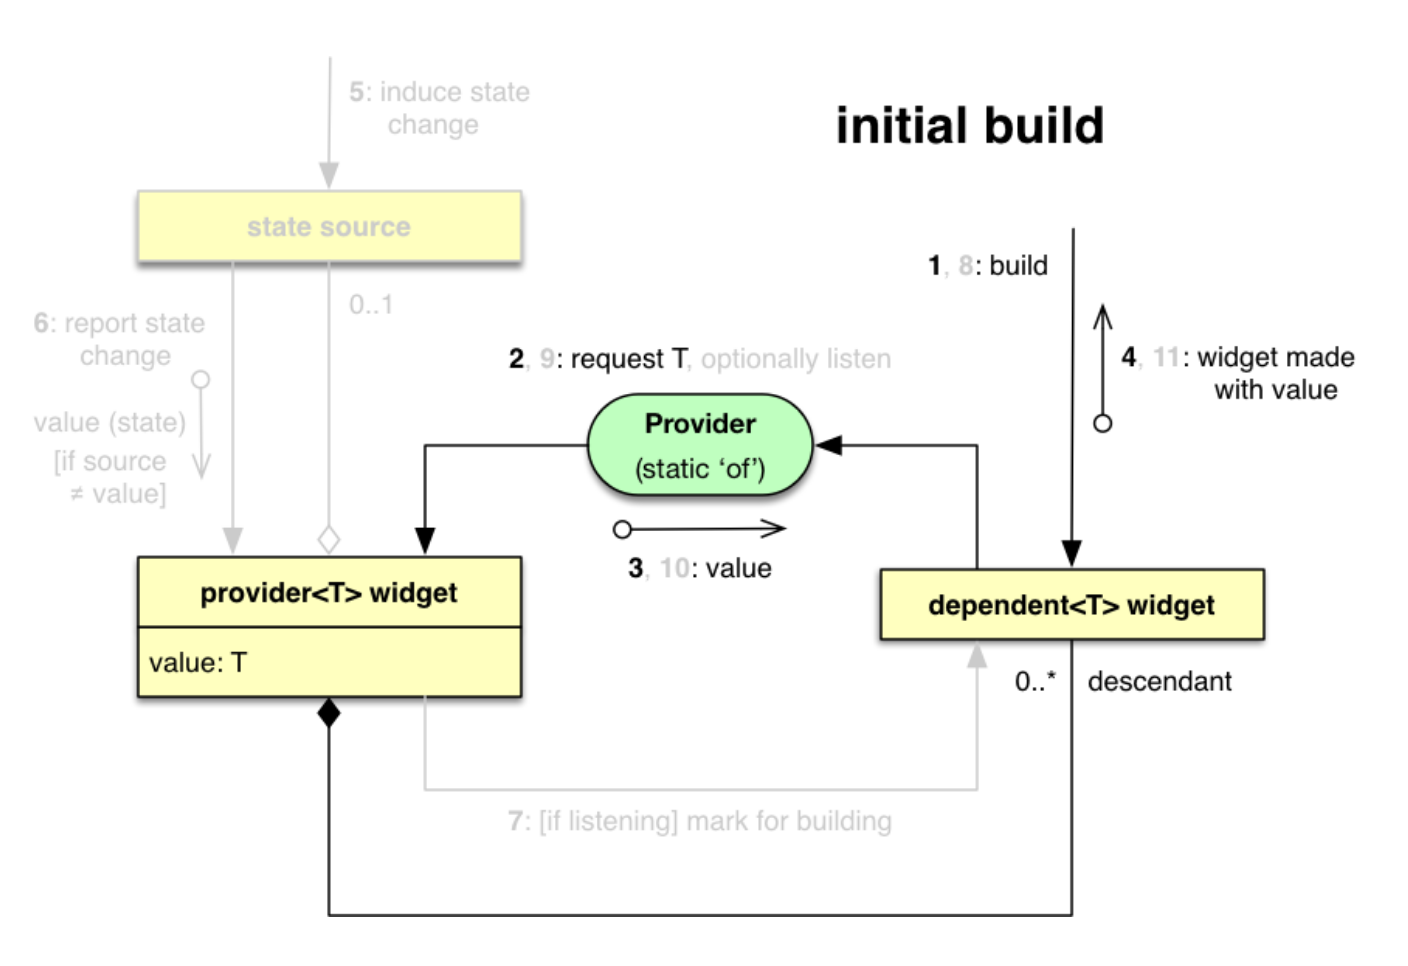
\includegraphics[scale=0.5]{provider_2}
		\caption[Provider - Inizializzazione]{Inizializzazione del Provider \cite{provider_first}.}
		\label{figura:provider_2}
	\end{center}
\end{figure}

I Widget possono riferirsi ai valori contenuti nel Provider con il metodo statico \verb|Provider.of<T>(context)|. Sulla base di questo metodo è possibile individuare un principale svantaggio di questo pattern: per poter recuperare i valori all'interno del Provider, è necessario che il metodo venga chiamato all'interno di un Widget (solitamente all'interno del metodo \verb|build()|) o che comunque gli venga passato un \verb|BuildContext context|. Questo svantaggio rappresenta una restrizione in quanto non è possibile utilizzare il Provider in classi dove non vi sia un \textit{contesto}. Ad esempio, il Provider non può essere utilizzato nelle classi che vanno a costituire la business logic.

Quando si va a definire e ad utilizzare un Provider, è necessario specificare il tipo di dato che il Provider deve rendere disponibile ai sui Widget discendenti. Questo significa che il Provider è una classe \textit{parametrica}: questo gli garantisce una certa flessibilità d'uso. Pertanto un Provider può rendere disponibile un valore di un qualsiasi tipo di dato.

Di seguito si introducono i passi che vengono svolti per poter istanziare il pattern:
\begin{enumerate}
	\item Come prima cosa Flutter si occupa della creazione del Provider. La costruzione del Provider implica la costruzione del figlio (\verb|child|) e la costruzione del figlio implica a sua volta la costruzione di tutti i Widget in esso contenuti. Il framework chiama il metodo \verb|build()| sul figlio per costruire il Widget che deve essere renderizzato. Questo metodo viene chiamato per tutti i Widget discendenti;
	\item Durante la compilazione (in particolare alla prima invocazione del metodo \verb|build()|), uno o più Widget discendenti, effettuano una chiamata al metodo \verb|Provider.of <T>()| per richiedere un valore. Questa chiamata viene fatta immediatamente dai Widget sottostanti, in quanto non possono essere creati senza un valore iniziale dello stato;
	\item Dopo che l'albero dei Widget è stato creato per la prima volta sulla base di uno stato iniziale, il Provider è in grado di ricevere i cambiamenti di stato. Al momento della ricostruzione dei Widget, il Provider crea un nuovo \verb|InheritedWidget| dalla stessa istanza del figlio utilizzata inizialmente. \verb|InheritedWidget| identifica i \textit{child} che stanno ascoltando i cambiamenti di stato e contrassegna soltanto i Widget che devono essere ricostruiti (Figura 6.2).
\end{enumerate}

\begin{figure}
	\begin{center}
		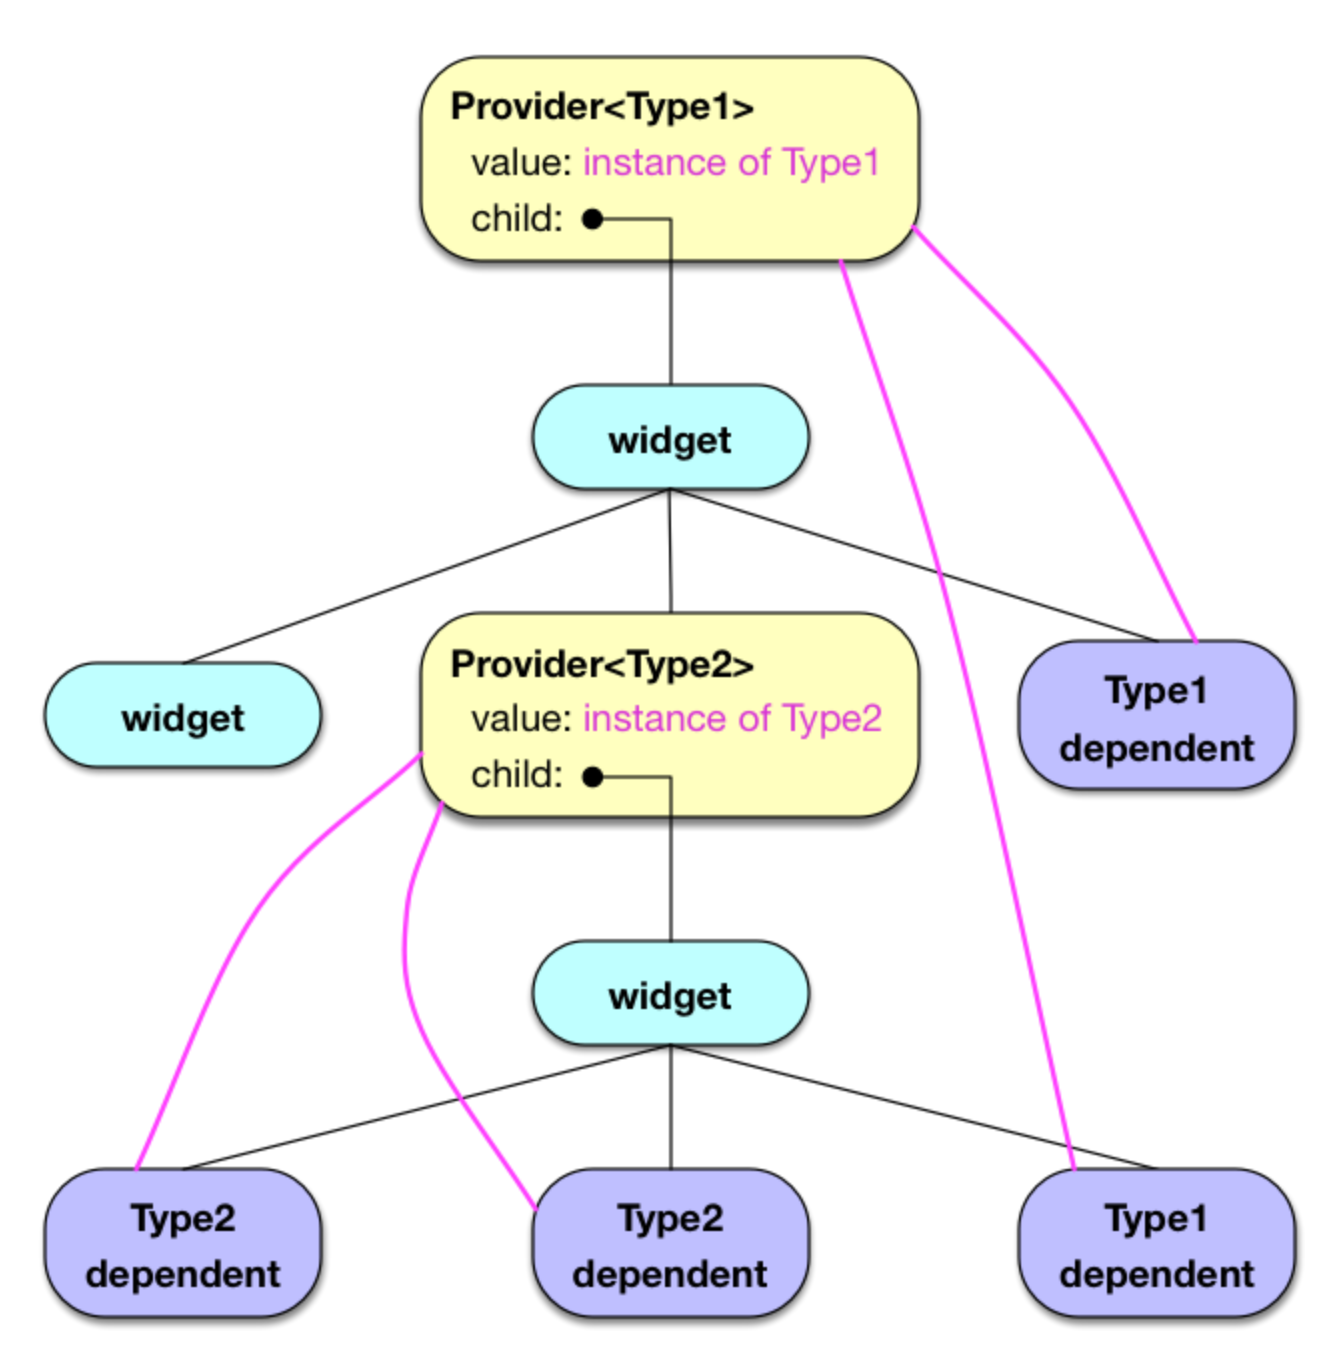
\includegraphics[scale=0.3]{provider_3}
		\caption[Provider - Aggiornamento]{Aggiornamento dei Widget a fronte di un cambiamento di stato \cite{provider_first}. Si può notare che non tutti i Widget vengono aggiornati ma soltanto quelli che hanno come "genitore" \textit{Provider.of \textless T \textgreater (context)}.}
		\label{figura:provider_3}
	\end{center}
\end{figure}

\label{consumer}
Nel momento in cui il Provider riceve un nuovo dato e lo deve rendere disponibile ai suoi discendenti, esso causerebbe il rendering di tutti i Widget sottostanti, anche di quelli che non sono influenzati dal cambiamento di stato. Pertanto, per ovviare a questa problematica, si può specificare esplicitamente quali Widget devono rimanere in ascolto per poter essere aggiornati di un nuovo cambiamento di stato (Figura 6.3). Ci sono vari modi per specificarlo:
\begin{enumerate}
	\item Chiamando il metodo \verb|Provider.of<T>(context)|;
	\item Utilizzando l'oggetto \verb|Consumer|
	\begin{lstlisting}
	Consumer<T>(
  		builder: (context, user, child) {
    			// Return a Widget tree
		}
	)
	\end{lstlisting}
\end{enumerate}

\begin{figure}
	\begin{center}
		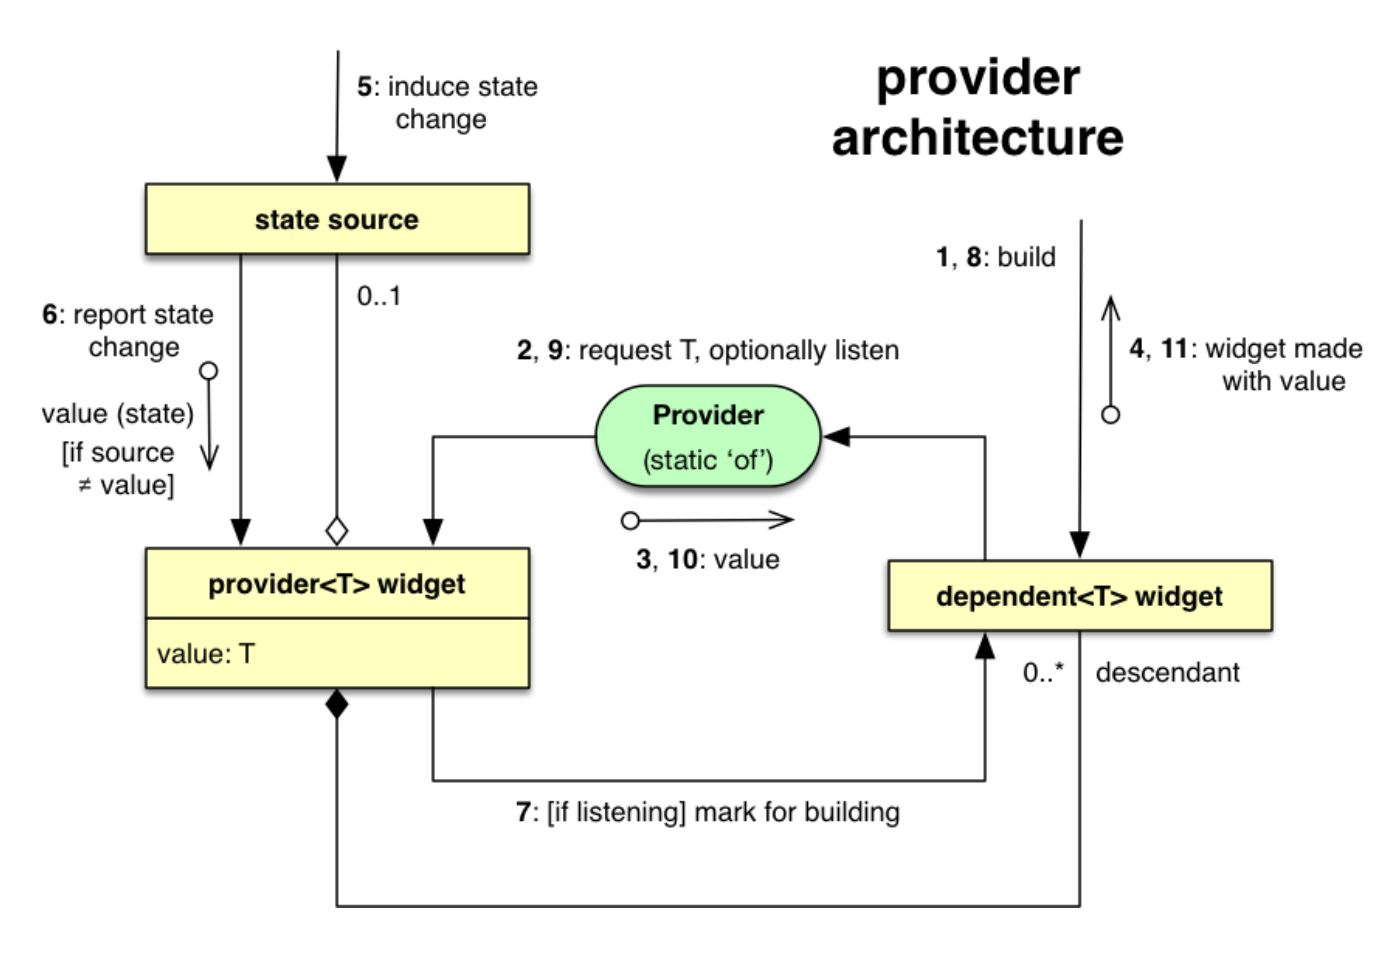
\includegraphics[scale=0.5]{provider}
		\caption[Provider - Architettura complessiva]{Architettura complessiva del pattern Provider\cite{provider_first}.}
		\label{figura:provider}
	\end{center}
\end{figure}

L'oggetto \verb|Consumer<T>| specifica che, al cambiamento di stato, deve essere aggiornato il Widget tree da quel punto in poi, evitando così di ricaricare i alcuni Widget immutabili. Queste tecniche permettono di non aggiornare eventuali Widget che si trovano a dei livelli superiori del Widget tree totale dell'applicazione, infatti, posizionare l'oggetto \verb|Consumer| o chiamare il metodo \verb|Provider.of<T>(context)| vicino alla radice del Widget tree complessivo, potrebbero provocare dei rallentamenti dell'applicazione. La problematica che nessuno di questi due metodi risolve è l'eventuale presenza di uno o più Widget che non devono essere aggiornati, ma che fanno comunque parte del sotto albero di \verb|Consumer| o di \verb|Provider.of<T>(context)|. È possibile ovviare a questo problema, specificando il valore del parametro \verb|listen| nel seguente modo: \verb|Provider.of<T>(context, listen: false)|. Così facendo, il Widget comunica al framework che è soltanto interessato a ricevere i dati dal Provider e che non necessita di essere ricostruito dal motore di rendering.

\subsubsection{Aggiornamento dello stato}
L'aggiornamento dello stato sfrutta i benefici che offre la programmazione reattiva. Possono venire utilizzati gli \verb|Stream|, i \verb|Future|, i \verb|ChangeNotifier| e i \verb|ValueNotifier|. Tutti questi oggetti permettono di comunicare istantaneamente i cambiamenti che rilevano. Così facendo, permettono di avere un flusso di dati che vengono resi disponibili al livello di presentazione dell'applicazione in tempo reale. L'\textit{aggiornamento dello stato} verrà descritto con maggior dettaglio nella spiegazione dedicata al pattern finale dell'applicazione.

\subsection{BLoC}
\subsubsection{Strutturazione del BLoC}
\begin{figure}
	\begin{center}
		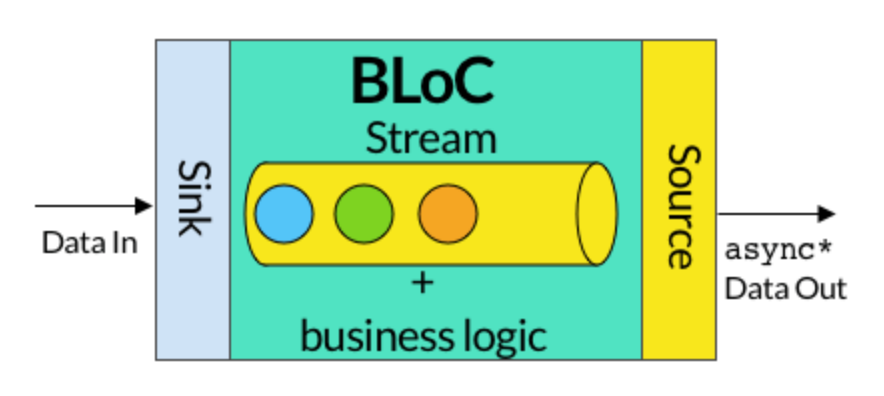
\includegraphics[scale=0.7]{bloc_architecture}
		\caption[BLoC - Architettura complessiva]{Architettura complessiva del pattern BLoC.}
		\label{figura:bloc_architecture}
	\end{center}
\end{figure}

Il \textbf{BLoC} è un sistema di \textit{state management}, consigliato dagli stessi sviluppatori di Google. Aiuta a gestire lo stato e ad accedere ai dati da una posizione centrale nel progetto. Questo pattern è stato presentato per la prima volta alla conferenza \textit{DartConf} del 2018 da parte da Google \cite{presentazione_bloc}. Tuttavia, Google non lo considera un pattern ufficiale per la realizzazione di applicazioni in Flutter, ma vuole semplicemente proporre un modello che può essere integrato con altre architetture o utilizzato singolarmente per lo sviluppo di app.

L'intento principale del pattern è quello di mantenere separata la \textbf{business logic} dall'\textbf{interfaccia grafica}. Non a caso, l'acronimo di BLoC è \textbf{Business Logic Components}. È uno dei pattern che vengono maggiormente utilizzati nella realizzazione di applicazioni in Flutter, in quanto permette di avere una struttura \textbf{scalabile} e \textbf{flessibile}. Anche questo pattern, come i precedenti, sfrutta la programmazione reattiva, sia per rilevare immediatamente un'interazione dell'utente, sia per propagare un nuovo stato ai vari Widget dell'applicazione.

Questo pattern può essere considerato come una \textit{pila}: l'entrata della pila si chiama \textbf{sink} e l’uscita si chiama \textbf{stream}. In entrata vengono accettati gli eventi generati dall’applicazione, come ad esempio un tap dell’utente, e in uscita viene ritornato uno stato che può essere utilizzato per propagare il cambiamento nell'albero dei Widget. Sulla base di questi due termini, si può intuire che l'oggetto principale che permette di rendere disponibile il flusso di dati è lo \verb|Stream|. La Figura 6.5 rappresenta graficamente le direzioni dei vari flussi all'interno del pattern.

I componenti principali di questo pattern sono due:
\begin{enumerate}
	\item UI: l'interfaccia grafica con cui l'utente può interagire;
	\item BLoC: la logica dell'applicazione che va a gestire gli eventi della UI e si collega a dei servizi esterni o a delle risorse interne (ad esempio, una API, cache ed altro ancora).
\end{enumerate}

Al verificarsi di un evento nell'interfaccia grafica, questo viene comunicato al BLoC (\textit{sink}), il quale elaborerà l'evento ed eventualmente apporterà un cambiamento di stato. Il BLoC, oltre a gestire gli eventi delle UI, fornisce i dati prelevati da dei servizi esterni e li invia all'interfaccia grafica. L'uso degli \verb|Stream| permette di sfruttare i vantaggi della programmazione reattiva, avendo così un'applicazione performante e reattiva. 

Lo \verb|Stream| viene istanziato dal BLoC (tramite l'oggetto \verb|StreamController|) e viene poi utilizzato dall'interfaccia grafica grazie al Widget \verb|StreamBuilder|. Nel \verb|child| dello \verb|StreamBuilder| viene associato tutto l'albero dei Widget che verrà aggiornato ogni volta che un nuovo dato sarà disponibile.

\begin{figure}
	\begin{center}
		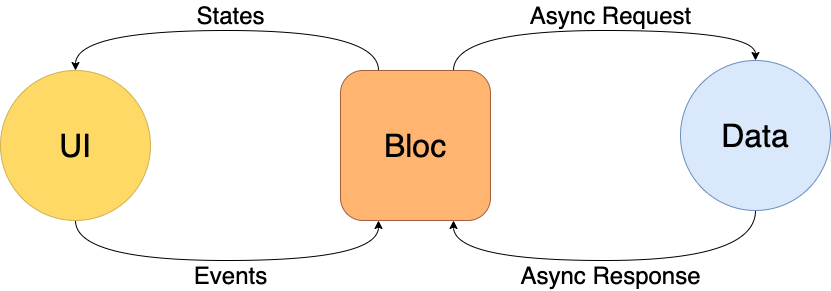
\includegraphics[scale=0.4]{bloc_architecture_2}
		\caption[BLoC - Flusso di dati e di eventi]{Rappresentazione del flusso di dati e di eventi.}
		\label{figura:bloc_architecture_2}
	\end{center}
\end{figure}

\subsubsection{Integrazione del pattern Provider}
Il BLoC è un componente che deve essere inserito nel Widget tree per poter essere usufruito. Pertanto, viene utilizzato il pattern \textit{Provider} a supporto del BLoC, il quale appunto permette di inserirlo all'interno dell'albero dei Widget. In particolare, il BLoC dovrà essere inserito prima dello \verb|StreamBuilder|, in quanto quest'ultimo dipende strettamente dallo \verb|Stream| dichiarato nel BLoC.

L'architettura così descritta definisce una struttura sufficientemente rigida da poter vincolare lo sviluppatore a seguire il flusso \textit{unidirezionale} dei dati. In questo modo, risulta più semplice focalizzarsi sulla realizzazione di un'interfaccia grafica reattiva, senza preoccuparsi della logica che deve essere implementata. Dualmente, nella business logic non è necessario conoscere come verrà realizzata l'interfaccia grafica: ci si concentra invece nel ricevere gli eventi dalla UI e in base ad essi, svolgere le azioni corrispondenti.

Un vincolo che è bene rispettare, è l'implementazione del metodo \verb|dispose()|. Questo metodo viene chiamato quando il BLoC deve essere deallocato e pertanto è necessario chiudere correttamente lo \verb|Stream|, per evitare di causare degli errori nell'applicazione. L'ambiente di sviluppo stesso (che sia Android Studio, IntelliJ, Visual Studio Code o altri) genera un \textit{warning} se nella classe del BLoC non viene mai chiuso lo \verb|Stream|.

Oltre alla rigidità della struttura, è concessa anche una certa flessibilità nella realizzazione dei componenti: un Widget complesso può essere scomposto in Widget più semplici, in modo che siano più facili da gestire e da riusare. Ogni Widget scomposto possiede il proprio BLoC. Quindi è possibile realizzare un componente, con il rispettivo BLoC, ed inserirlo in differenti schermate dell'applicazioni con molta facilità.

Questa architettura impone il rispetto di una regola fondamentale: \textbf{non è possibile condividere} lo stesso BLoC per Widget differenti. Questo dubbio può sorgere allo sviluppatore in situazioni in cui si verifica la necessità di condividere gli stessi dati a due o più Widget differenti contemporaneamente. Risulta naturale, in tale situazione, collegare tutti i Widget sotto un unico BLoC. Tuttavia questa \textit{non è una buona pratica} di programmazione. La condivisone di un BLoC per più schermate può generare diverse problematiche, ad esempio:
\begin{enumerate}
	\item L'aggiornamento di una schermata provoca l'aggiornamento anche delle altre schermate, anche quando non vi è bisogno;
	\item Nel momento in cui viene chiamato il metodo \verb|dispose()|, il BLoC viene deallocato per tutte le schermate con cui è stato condiviso. Quindi navigando tra le schermate, dopo che il BLoC è stato deallocato, si possono verificare degli errori e dei \textit{crash} dell'applicazione.
\end{enumerate}

Un vantaggio dell'integrazione del Provider nel pattern BLoC, è la possibilità di poter istanziare soltanto una volta il BLoC. Una volta istanziato, questo può essere utilizzato in qualsiasi punto dell'applicazione, purché vi sia un \verb|context|. Così facendo, è possibile avere un'ottima flessibilità dell'architettura, evitando di istanziare più volte lo stesso oggetto durante il ciclo di vita dell'applicazione e potendolo utilizzare con una certa facilità, quando lo si necessita.

\subsection{Motivazioni della scelta}
È stato scelto di utilizzare il pattern \textit{BLoC} in quanto l'ho confrontato con le altre architetture disponibili e sono giunto alla conclusione che fosse il pattern ideale per la realizzazione di questa applicazione. Viene sfruttata appieno la programmazione reattiva, caratteristica peculiare del linguaggio, e fornisce una struttura rigida. La rigidità dell'architettura permette di creare delle applicazioni chiare dal punto di vista strutturale. Inoltre permette di avere una certa flessibilità per l'implementazione di funzionalità future.

\section{Architettura proposta}
In questo paragrafo vengono spiegate le problematiche dell'architettura BLoC e le motivazioni che hanno portato a dover attuare delle opportune modifiche per soddisfare i requisiti dell'applicazione.

\subsection{Problematiche del pattern BLoC}
L'applicazione che deve essere realizzata richiede di accedere a dei dati che devono essere forniti da un server, tramite una socket. Questi dati devono essere condivisi tra più schermate: in particolare, si avrà una schermata generale (una \textit{dashboard}), per avere un quadro generale di tutti i dati, e poi vi saranno delle schermate specifiche, che illustreranno soltanto un piccolo set di dati. Tutte queste schermate attingono da un'unica fonte di dati: dalla socket.

Come è stato discusso precedentemente, non è possibile condividere un BLoC per più schermate contemporaneamente. Pertanto, si è dovuti procedere a modificare l'architettura proposta dalla comunità di Flutter, per poterla adattare alle esigenze richieste.

\subsection{Introduzione del Repository pattern}
Per poter risolvere le limitazioni del BLoC, viene integrato il \textbf{Repository} pattern \cite{repository_pattern}. Una spiegazione del Repository è stata data da Martin Fowler nel libro \textit{Patterns of Enterprise Application Architecture}. L'autore spiega che un "\textit{Repository incapsula l'insieme di oggetti persistenti in un archivio dati e le operazioni eseguite su di essi, fornendo una vista più orientata agli oggetti del livello di persistenza.}" Il Repository permette anche di ottenere una netta separazione e una dipendenza unidirezionale tra il dominio e i livelli di mappatura dei dati. Questa concezione è nata in un periodo in cui le applicazioni \textit{enterprise} necessitavano ridurre la duplicazione della logica delle query.

Tuttavia, nel tempo, le esigenze delle applicazioni sono cambiate, in particolare per le applicazioni mobili. In questo contesto, il concetto di Repository viene inteso più come un componente che si interfaccia con un archivio esterno (in generale, qualsiasi altro servizio esterno all'applicazione). In questo caso, il Repository ha il compito di nascondere l'implementazione della logica che permette di interfacciarsi con i servizi esterni. Così facendo, la struttura dell'applicazione risulta essere più flessibile per le modifiche future dei requisiti e il conseguente \textit{refactoring}.

Si possono notare delle differenze sostanziali tra le due definizioni. Per la realizzazione dell'applicazione è stata presa in considerazione l'ultima definizione descritta, le cui motivazioni verranno esposte nella sezione successiva.

\subsection{Architettura modificata}
L'architettura proposta per l'applicazione è costituita dall'integrazione del pattern \textbf{BLoC} con il \textbf{Repository} pattern. Come è stato illustrato precedentemente, nella versione base, il BLoC si occupa di interfacciarsi con la UI da un lato e con i servizi esterni dall'altro. Per sopperire alla problematica della condivisione dei dati ricevuti dalla socket tra le diverse schermate, viene introdotto un Repository tra il BLoC e i servizi esterni. Così facendo si possono ottenere i seguenti vantaggi:
\begin{enumerate}
	\item In questo modo, è possibile utilizzare il Repository come punto di riferimento per la ricezione dei dati per i BLoC. Ovvero, i vari BLoC possono collegarsi ad un Repository comune a tutti e possono ricevere i dati filtrati dal Repository stesso. Infatti, il Repository permette di astrarre dalla sorgente di dati esterna: i BLoC devono soltanto interfacciarsi con il Repository per ottenere i dati, senza preoccuparsi se questi provengano da una socket, da un'API, dalla memoria interna del dispositivo o da qualsiasi altra fonte di dati. Il Repository si preoccupa di interfacciarsi con tali servizi e di confezionare in un certo formato i dati ricevuti, per renderli disponibili e comprensibili ai vari BLoC che vi si collegano;
	\item Grazie a questo nuovo livello di astrazione, tutta la business logic viene alleggerita dal carico di lavoro sostenuto per connettersi ai servizi esterni. Infatti, nel caso in cui in futuro si dovrà cambiare il servizio che permette di ottenere i dati navali, bisognerebbe andare a modificare il codice di ogni singolo BLoC che è stato creato. L'utilizzo invece del Repository, toglie questa responsabilità ai BLoC ed esso diventa l'unico "servizio" a cui i BLoC si devono collegare.
\end{enumerate}

Uno svantaggio dell'integrazione di queste due architetture è appunto l'introduzione di un nuovo livello di astrazione, ovvero, l'introduzione di \textit{overhead}. Per ridurre al minimo questa possibile problematica, viene in aiuto la programmazione reattiva con l'utilizzo degli \textit{flussi} (\verb|Stream| o \verb|ValueNotifier|). Altro fattore che permette di minimizzare questo problema è quello di ridurre al minimo il lavoro che deve svolgere il Repository. I compiti che deve svolgere sono:
\begin{enumerate}
	\item Connettersi con la socket;
	\item Ricevere i dati;
	\item Confezionare i dati ricevuti in un oggetto comprensibile da parte di tutti i BLoC;
	\item Trasmettere i dati in uno \verb|Stream|.
\end{enumerate}

Il lavoro di selezione dei dati viene effettuato dai singoli BLoC, rendendo più veloce il passaggio dei dati dalla sorgente fino ai vari componenti della business logic.

\section{Architettura implementata}
\label{architettura implementata}
Nei paragrafi precedenti, si è andati a descrivere nel particolare le varie architetture, illustrando le motivazioni per cui sono state scelte. Sono state esposte le varie problematiche ed è stata proposta una nuova versione dell'architettura. In questo paragrafo verrà mostrata l'architettura complessiva implementata nell'applicazione.

\subsection{Descrizione}
\begin{figure}
	\begin{center}
		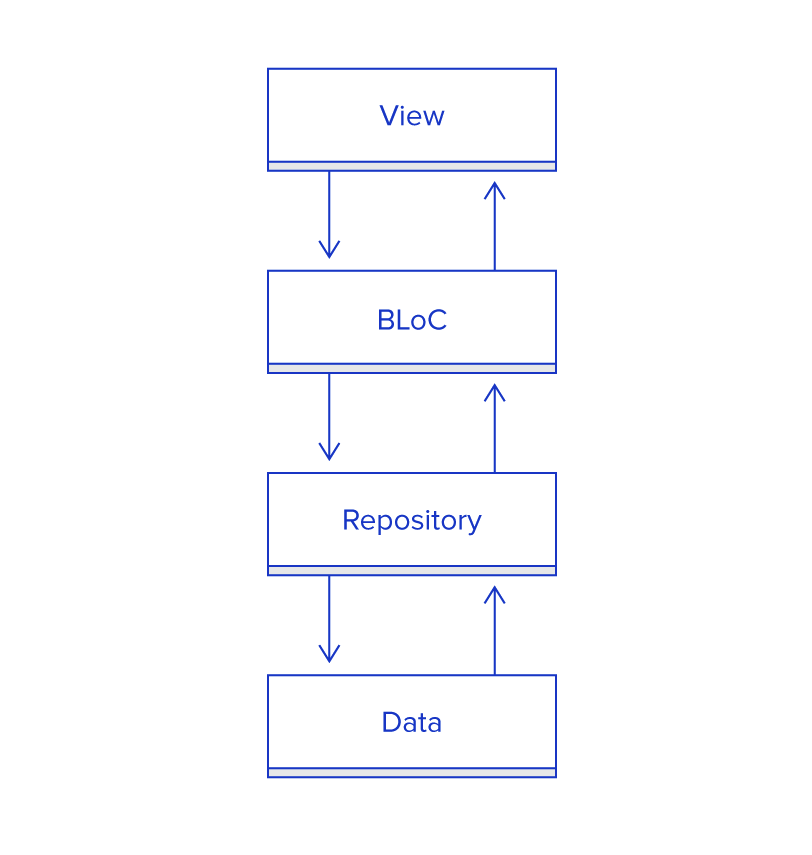
\includegraphics[scale=0.29]{architettura_implementata}
		\caption[Architettura implementata]{Illustrazione degli strati dell'architettura implementata.}
		\label{figura:architettura_implementata}
	\end{center}
\end{figure}

Sulla base di tutte le nozioni che sono state fornite precedentemente, si è giunti ad una struttura finale dell'architettura dell'applicazione. In particolare, gli strati dell'architettura sono (Figura 6.6 \cite{architettura_implementata}):
\begin{enumerate}
	\item \textbf{Interfaccia grafica} (\textbf{View}): tutti quei componenti grafici con cui l'utente può interagire e visualizzare le informazioni richieste;
	\item \textbf{BLoC}: lo strato in cui è contenuta la logica dell'applicazione. Lo logica totale dell'app è data dall'insieme di tutti i BLoC delle singole schermate e dei singoli Widget;
	\item \textbf{Repository}: un livello che si occupa di astrarre il \textit{link} tra i BLoC e i servizi esterni;
	\item \textbf{Servizi esterni}: in questo caso, sono rappresentati dalla socket. In futuro, altri servizi che potrebbero essere inseriti sono, ad esempio, un'API o anche i dati GPS provenienti dal sensore installato sul dispositivo mobile.
\end{enumerate}

\subsection{Integrazione del Repository}
Nell'architettura di base del BLoC, le classi che implementavano la business logic si occupavano di andare a richiedere i dati ai vari servizi esterni. Ora, invece, i vari BLoC si collegano al Repository, che fa da intermediario tra i servizi esterni e i BLoC stessi. L'aggiunta di uno strato ulteriore implica la modifica della modalità di comunicazione tra i BLoC e i servizi. Con il Repository, la comunicazione avviene nel seguente modo;
\begin{enumerate}
	\item Il Repository si collega ai vari servizi esterni, effettua una richiesta sulla base di un particolare evento ricevuto, riceve la risposta e la inoltra in un \verb|ValueNotifier<T>|. Un \verb|ValueNotifier<T>| può essere usato per contenere un singolo valore e avvisare i suoi ascoltatori quando questo cambia;
	\item Al \verb|ValueNotifier<T>| del Repository, si collegano tutti i BLoC di cui necessitano i dati provenienti da questo strato;
	\item Nei BLoC viene inizializzato un \textit{ascoltatore}, che alla ricezione di un nuovo dato nel \verb|ValueNotifier<T>|, chiama una funzione, passandogli come parametro il dato appena ricevuto;
	\item Una volta ricevuto il dato, la funzione del BLoC specifico elimina i dati di cui non necessita (il Repository fornisce tutti i dati provenienti dalla socket) e li propaga nell'interfaccia grafica. La comunicazione tra la UI e i BLoC avviene tramite \verb|Stream|: la comunicazione tra questi due strati non è cambiata dalla versione base del pattern.
\end{enumerate}

L'implementazione dell'architettura così descritta, permette di \textbf{astrarre} dal tipo di servizio che viene utilizzato e permette anche di avere un \textbf{punto di riferimento per la distruzione dei dati} ai vari BLoC. Tutte queste caratteristiche rendono l'architettura adatta per l'applicazione che deve essere implementata.

Per quanto riguarda il passaggio dei dati tra il Repository e i BLoC, si è deciso di non inviare i dati ai BLoC già convertiti e pronti per essere utilizzati. Il motivo è quello di non \textit{sovraccaricare} il Repository, in quanto causerebbe il degrado delle prestazioni. Così facendo, il carico di lavoro viene distribuito tra il Repository e i BLoC.

L'integrazione del Repository pattern nell'architettura avviene grazie all'utilizzo del \textit{Provider}. È possibile fare un discorso analogo a quello che è stato fatto per l'integrazione del Provider nel BLoC. Essendo un componente di \textit{fondamentale} importanza, il Repository viene posto vicino alla radice dell'albero dell'applicazione: venendo utilizzato da diverse schermate durante il ciclo di vita dell'applicazione, nel momento in cui avviene la chiusura dell'app, il Repository sarà uno degli ultimi oggetti che verranno deallocati. In questo modo, le schermate non saranno soggette ad errori, in quanto queste verranno deallocate prima del Repository.

\section{Descrizione dettagliata dell'architettura implementata}
In questa sezione si procede a descrivere dettagliatamente l'architettura implementata, a partire dai componenti più interni, per procedere poi a trattare le parti che gestiscono l'interazione con l'utente.

\subsection{Organizzazione delle classi e dei package}
In questa breve sezione, viene illustrata l'organizzazione dei package e delle varie classi dell'applicazione realizzata.

L'applicazione è stata strutturata seguendo gli strati dell'architettura, ovvero, è stato creato un package per ogni livello dell'architettura.

L'applicazione è stata organizzata nel seguente modo (in ordine alfabetico):
\begin{enumerate}
	\item \textbf{blocs}
		\begin{enumerate}
			\item dashboard
				\begin{enumerate}
					\item \textit{dashboard\_widget\_bloc.dart}
				\end{enumerate}
			\item gps
				\begin{enumerate}
					\item \textit{gps\_bloc.dart}
				\end{enumerate}
			\item location
				\begin{enumerate}
					\item \textit{location\_bloc.dart}
				\end{enumerate}
			\item navigation
				\begin{enumerate}
					\item \textit{navigation\_bloc.dart}
				\end{enumerate}
			\item wind
				\begin{enumerate}
					\item \textit{wind\_bloc.dart}
				\end{enumerate}
			\item \textit{bloc.dart}
		\end{enumerate}
	\item \textbf{models}
		\begin{enumerate}
			\item repository
				\begin{enumerate}
					\item \textit{repository\_data\_model.dart}
					\item \textit{timestamp.dart}
				\end{enumerate}
			\item settings
				\begin{enumerate}
					\item cache
						\begin{enumerate}
							\item \textit{cache.dart}
						\end{enumerate}
					\item server
						\begin{enumerate}
							\item \textit{server\_parameters.dart}
							\item \textit{server\_settings.dart}
							\item \textit{server\_settings\_file.dart}
						\end{enumerate}
				\end{enumerate}
			\item ui
				\begin{enumerate}
					\item \textit{base\_model.dart}
					\item \textit{dashboard.dart}
					\item \textit{gps.dart}
					\item \textit{location.dart}
					\item \textit{navigation.dart}
					\item \textit{wind.dart}
				\end{enumerate}
			\item \textit{acronyms.dart}
		\end{enumerate}
	\item \textbf{repositories}
		\begin{enumerate}
			\item \textit{repository\_socket.dart}
		\end{enumerate}
	\item \textbf{services}
		\begin{enumerate}
			\item \textit{socket\_service.dart}
		\end{enumerate}
	\item \textbf{ui}
		\begin{enumerate}
			\item common\_widgets
				\begin{enumerate}
					\item app\_bar
						\begin{enumerate}
							\item \textit{page\_app\_bar.dart}
							\item \textit{sensor\_data\_app\_bar.dart}
						\end{enumerate}
					\item grid\_box
						\begin{enumerate}
							\item \textit{grid\_box\.widget.dart}
						\end{enumerate}
					\item location
						\begin{enumerate}
							\item \textit{location\_widget.dart}
						\end{enumerate}
				\end{enumerate}
			\item pages
				\begin{enumerate}
					\item dashboard
						\begin{enumerate}
							\item widgets.\textit{dashboard\_widget.dart}
							\item \textit{dashboard\_page.dart}
						\end{enumerate}
					\item gps
						\begin{enumerate}
							\item \textit{gps\_page.dart}
						\end{enumerate}
					\item navigation
						\begin{enumerate}
							\item \textit{navigation\_page.dart}
						\end{enumerate}
					\item settings
						\begin{enumerate}
							\item cache.\textit{cache\_page.dart}
							\item server.\textit{server\_page.dart}
							\item theme.\textit{theme\_page.dart}
							\item \textit{settings\_page.dart}
						\end{enumerate}
					\item wind
						\begin{enumerate}
							\item \textit{wind\_page.dart}
						\end{enumerate}
				\end{enumerate}
		\end{enumerate}
	\item \textbf{utils}
		\begin{enumerate}
			\item ui
				\begin{enumerate}
					\item themes
						\begin{enumerate}
							\item \textit{custom\_theme.dart}
							\item \textit{default\_theme.dart}
							\item \textit{high\_contrast\_theme.dart}
							\item \textit{theme\_handler.dart}
							\item \textit{themes.dart}
						\end{enumerate}
					\item \textit{colors\_palette.dart}
				\end{enumerate}
		\end{enumerate}
	\item \textbf{\textit{main.dart}}
\end{enumerate}

\subsection{Modelli}
In questa sezione vengono descritti tutti i modelli utilizzati dai vari strati dell'applicazione.

\subsubsection{Acronyms}
Questa è una semplice classe contente delle mappe \textit{acronimo - nome del dato} che vengono utilizzate nelle schermate dell'applicazione. I dati forniti dalla socket sono espressi sotto forma di \textit{acronimi}. Tuttavia in alcune sezioni dell'applicazione è preferibile avere il nome completo del dato che si sta osservando.

La mappa che contiene le associazioni tra acronimi e nomi dei dati dei sensori è la seguente:

\lstset{numbers=left, % vogliamo numerare le righr
  numberstyle=\tiny, % i numeri sono piccoli
  basicstyle=\ttfamily, % usiamo il carattere dattilografico
  columns=fullflexible, % niente emulazioni di allineamento
  backgroundcolor=\color{lightgray}, % colore di sfondo
  language=Java, % linguaggio usato
  }
  \begin{lstlisting}
  static final Map<String, String> _acronyms = {
   	"aws":	"Apparent Wind Speed",
	"awa":       "Apparent Wind Angle",
    	"sog":        "Speed Over Ground",
    	"cog":        "Curse Over Ground",
    	"mh":         "Magnetic Heading",
    	"sow":       "Speed Over Water",
    	"tws":        "True Wind Speed",
    	"twa":        "True Wind Angle",
    	"ih":           "imu_heading",
    	"cang":      "calypso_ang",
    	"camp":     "calypso_amp",
    	"nwang":   "nwang",
  };
  \end{lstlisting}

Tramite il seguente metodo, dato un acronimo, è possibile ottenere il nome completo del dato corrispondente:
\begin{lstlisting}
  static String getSentence(String acronym) {
  	return _acronyms[acronym];
  }
  \end{lstlisting}

\subsubsection{RepositoryDataModel}
Questo oggetto viene utilizzato per incapsulare i dati ricevuti dalla socket. Grazie a questo oggetto è possibile poi trasmetterlo al Repository e ai vari BLoC.

Si può notare dal commento, che l'introduzione di un oggetto \verb|Timestamp| sarà necessario per dei sviluppi futuri, ad esempio, la realizzazione di grafici per i vari sensori. Il timestamp è già presente ogni volta che viene fatta una richiesta alla socket e vengono ricevuti dei dati. Inoltre il timestamp è già presente nella \textit{cache}: è sufficiente utilizzarlo in quanto l'implementazione effettiva è già stata predisposta.

L'oggetto \verb|Timestamp| contiene delle informazioni riguardanti l'ora, il minuto e il secondo in cui i dati sono stati ricevuti dalla socket.

  \begin{lstlisting}
  class RepositoryDataModel {
  	final String jsonData;
  	final Timestamp timestamp;
  	// I need this to know what time I requested the data  
  	// from the socket, so in this way I can build a chart

  	RepositoryDataModel({@required this.jsonData, 
  	@required this.timestamp});

  	@override
  	String toString() {
    		return jsonData + "\n" + timestamp.toString();
  	}
  }
  \end{lstlisting}
  
\subsubsection{BaseModel}
Questa \textit{classe astratta} rappresenta un riferimento comune per tutti i modelli delle specifiche schermate. Per ogni schermata viene associato un particolare modello, nei quali vengono salvati soltanto un piccolo set dei dati forniti dal Repository.

L'unico metodo che dovrà essere implementato dai vari modelli che estenderanno questa classe astratta, è il metodo \verb|toMap()|, che permette alla classe di restituire i dati che essa contiene, sotto forma di una mappa.

\begin{lstlisting}
abstract class BaseModel {
  	Map<String, dynamic> toMap();
}
\end{lstlisting}

\subsubsection{Dashboard}
Il modello che verrà illustrato è il modello che contiene il maggior numero di campi, in quanto la schermata \textit{Dashboard} ha il compito di mostrare all'utente un quadro generale della situazione, presentando tutti i dati ricevuti dal Repository.

Il metodo \verb|Dashboard.fromJson(Map<String, dynamic> json)| estrapola tutti i dati di cui necessita, da un particolare oggetto che li contiene. Questo metodo viene chiamato nel momento in cui vengono ricevuti i dati dal Repository, che sono salvati in formato JSON.

I modelli \verb|Navigation|, \verb|GPS| e \verb|Wind| sono molto simili al modello che è stato presentato. Variano soltanto per numero e tipologia di dati memorizzati al loro interno.

Il modello \verb|Location| è molto simile al modello \verb|Dashboard|, con l'unica differenza che non viene implementato il metodo \verb|fromJson|. Il motivo è che i dati vengono già decodificati dal JSON e vengono poi passati direttamente a tale modello.

\begin{lstlisting}
class Dashboard extends BaseModel {
  final String apparentWindSpeed;
  final String apparentWindAngle;
  final String speedOverGround;
  final String curseOverGround;
  final String magneticHeading;
  final String speedOverWater;
  final String trueWindSpeed;
  final String trueWindAngle;
  final String imu_heading;
  final String calypso_ang;
  final String calypso_amp;
  final String nwang;

  // Constructor
  Dashboard({
    this.apparentWindSpeed = "0",
    this.apparentWindAngle = "0",
    this.speedOverGround = "0",
    this.curseOverGround = "0",
    this.magneticHeading = "0",
    this.speedOverWater = "0",
    this.trueWindSpeed = "0",
    this.trueWindAngle = "0",
    this.imu_heading = "0",
    this.calypso_ang = "0",
    this.calypso_amp = "0",
    this.nwang = "0",
  });

  factory Dashboard.fromJson(Map<String, dynamic> json) {
    return Dashboard(
      apparentWindSpeed: json['aws'],
      speedOverGround: json['sog'],
      curseOverGround: json['cog'],
      magneticHeading: json['mh'],
      speedOverWater: json['sow'],
      trueWindSpeed: json['tws'],
      trueWindAngle: json['twa'],
      imu_heading: json['imu_heading'],
      calypso_ang: json['calypso_ang'],
      calypso_amp: json['calypso_amp'],
      nwang: json['nwang'],
    );
  }

  @override
  Map<String, dynamic> toMap() {
  	...
  }
\end{lstlisting}

\subsubsection{Cache}
Questo modello permette di salvare i dati che vengono ricevuti dalla socket. I dati vengono salvati nella \textit{cache} dal Repository. Le varie schermate utilizzano la cache nella loro fase di inizializzazione, ovvero, recuperano l'ultimo dato salvato per poter istanziare correttamente tutti i componenti della schermata.

La \verb|Cache| è una classe parametrica, quindi è possibile utilizzarla in qualsiasi contesto e con qualsiasi tipo si desideri. I vari dati vengono memorizzati in una lista. I metodi che supporta questa classe sono:
\begin{enumerate}
	\item \verb|save(T data)|: questo metodo si interfaccia con la lista interna e permette di salvare un nuovo dato in tale lista;
	\item \verb|void emptyCache()|: questo metodo permette di svuotare la cache;
	\item \verb|bool isCacheEmpty()|: permette di verificare se la lista interna è vuota o meno;
	\item \verb|T _getLastDataCached()|: è un metodo interno alla classe e permette di ottenere l'ultimo dato che è stato salvato nella lista;
	\item \verb|get lastData|: è un metodo pubblico che utilizza \verb|_getLastDataCached()|. Non è stato utilizzato direttamente il metodo privato in quanto si voleva rendere il nome del metodo più intuitivo;
	\item \verb|List<T> _getDataCached ()|: questo metodo privato permette di ottenere tutto il contenuto della cache;
	\item \verb|get dataCached|: è un metodo pubblico che chiama \verb|_getDataCached ()|. Le motivazioni della creazione di questo metodo sono analoghe a quelle del metodo \verb|get lastData|;
	\item \verb|get size|: questo metodo permette di ottenere quanti dati sono stati salvati nella cache, ovvero, nella lista.
\end{enumerate}

\subsubsection{ServerParameters}
Questa classe permette di salvare tutti i dati necessari per effettuare la connessione al server (indirizzo IP e porta) e per implementare il \textit{polling} (un numero intero che rappresenta l'intervallo di tempo, espresso in secondi). La classe in questione, viene utilizzata dalla schermata \textit{Server}, nella quale è possibile aggiornare i parametri di connessione e del polling. Pertanto, vi sono diversi metodi che vanno ad analizzare i diversi input, in formato stringa, per controllare che rispettino i tipi e i formati richiesti.

\subsubsection{ServerSettingsFile}
Questa classe ha un ruolo di interfaccia tra l'applicazione ed un file di configurazione in JSON. In questo file vengono memorizzati tutti i dati relativi alla connessione e al polling. Così facendo, al riavvio dell'applicazione, se sono state effettuate delle modifiche a tali parametri, questi non vengono persi e possono essere ricaricati.
Le operazioni supportate da questa classe sono:
\begin{enumerate}
	\item \verb|static Future<String> readSettings()|: operazione per leggere dal file JSON;
	\item \verb|static Future<File> writeSettings(String serverSettings)|: metodo che permette di scrivere i dati sul file JSON.
\end{enumerate}

Vengono utilizzati degli oggetti \verb|ServerSettings| per incapsulare tutti i dati che devono essere memorizzati nel file.

\subsubsection{ServerSettings}
Questa classe contiene i medesimi parametri della classe \verb|ServerParameters| e viene utilizzata dalla classe \verb|ServerSettingsFile|. L'oggetto ottenuto per istanziazione di questa classe, possiede un metodo per \textit{codificare} i dati in JSON (\verb|Map<String, dynamic> toJson()|) , in modo da poterli memorizzare nel file, e un metodo per \textit{decodificare} i dati dal file JSON \\(\verb|factory ServerSettings.fromJson(Map<String, dynamic> json)|), in modo da renderli disponibili ai livelli superiori dell'applicazione.

\subsection{Socket}
La \textit{socket} che viene fornita dal server \textit{Argos} tramite la porta \textit{4545}, rappresenta il servizio esterno da cui l'applicazione prende i dati necessari. Nel caso in cui in futuro, i medesimi dati vengano resi disponibili tramite un altro software o un'altra metodologia, sarà sufficiente creare una nuova classe o un nuovo modulo che implementi la connessione al servizio e i metodi per ottenere i dati da tale servizio.

\subsubsection{Metodo getData()}
Questo metodo permette di connettersi ad una socket e di ottenere i dati da essa. Secondo il protocollo che è stato realizzato nel server \textit{Argos}, una volta che il client effettua una richiesta al server, il server invia la risposta e chiude immediatamente la socket. Pertanto, una volta ricevuti i dati (da riga 10 a riga 15), la socket deve essere chiusa correttamente anche dal lato del client (riga 17).

Il metodo appena descritto è un metodo \textit{asincrono}, ovvero, l'applicazione non viene bloccata fino a quando non vengono ricevuti i dati, ma è possibile svolgere altre azioni. Nel caso ci fossero delle problematiche con la connessione ad Internet, l'implementazione che è stata attuata permette di non bloccare l'applicazione.

Il tipo di ritorno è un \verb|Future<RepositoryDataModel>|: \verb|Future| perchè è un metodo asincrono, e \verb|RepositoryDataModel| perchè i dati ricevuti dalla socket vengono incapsulati in un oggetto comune che possa essere comprensibile ai vari BLoC che si collegheranno al Repository. Incapsulare i dati già in questo strato dell'applicazione permette di alleggerire il carico di lavoro del Repository.

  \begin{lstlisting}
  Future<RepositoryDataModel> getData() async {
    Completer<RepositoryDataModel> repositoryData =
        Completer<RepositoryDataModel>();

    try {
      Socket socket = await Socket.connect(serverIPAddress, 
      serverPort, timeout: Duration(seconds: 2));
      log("Socket connected", name: "SailingSocket");

      socket.listen((data) async {
        repositoryData.complete(RepositoryDataModel(
          jsonData: String.fromCharCodes(data).trim(),
          timestamp: Timestamp(dateTime: DateTime.now()),
        ));
      });

      socket.close();
      log("Socket closed", name: "SailingSocket");
    } on SocketException catch (e) {
      rethrow;
    } on TimeoutException catch (e) {
      rethrow;
    }
    return repositoryData.future;
  }
  \end{lstlisting}

\subsection{Repository}
Come è già stato descritto precedentemente, il Repository è uno strato che si interpone tra i BLoC e i vari servizi esterni. Il compito del Repository è quello di nascondere come avviene la connessione con i servizi esterni. Questi possono essere dei \textit{Web services}, una socket o qualsiasi altra fonte di dati. In questo modo, gli altri componenti utilizzano un'interfaccia unica per connettersi al Repository, indipendentemente dalla tipologia di servizio che viene usufruito.

La scelta di introdurre un ulteriore strato all'architettura originale è dovuta anche ad una caratteristica intrinseca del progetto. Un requisito dell'applicazione consiste nell'interrogare periodicamente (eseguire un \textit{polling}) la socket, in modo da avere i dati sempre aggiornati. Inoltre, tutte le schermate dell'applicazione attingono i dati dalla medesima fonte. Non potendo condividere i BLoC per più schermate, la soluzione del Repository risulta essere la scelta più ragionevole. Quindi, nel Repository viene svolto il \textit{polling}, ovvero, periodicamente vengono effettuate delle richieste alla socket sulla base di un parametro che indica quanti secondi devono essere attesi tra una richiesta e quella successiva.

Da un punto di vista più approfondito, nel Repository è presente:
\begin{enumerate}
	\item \verb|ValueNotifier<RepositoryDataModel>|: permette di sfruttare la programmazione reattiva, comunicando, a tutti gli oggetti connessi al Repository, i dati trasmessi attraverso questo oggetto;
	\item \verb|start()|: questo metodo viene invocato nella schermata \textit{Dashboard} e permette di inizializzare il \textit{polling} del servizio;
	\item \verb|stop()|: questo metodo permette di fermare il polling. Viene invocato dall'utente grazie all'interazione con la schermata \textit{Dashboard};
	\item \verb|_getDataFromSocket()|: è un metodo privato (in Dart vengono identificati con il carattere di \textit{underscore}, '\_') che va ad effettuare esplicitamente la chiamata al servizio esterno. Una volta ricevuto il dato, questo viene tramesso nel \verb|ValueNotifier<RepositoryDataModel>|;
	\item \verb|dispose()|: è un metodo che viene invocato nel momento in cui viene deallocato il Repository. È buona pratica chiudere correttamente gli \verb|Stream| e i \verb|ValueNotifier<T>| per evitare che il canale di comunicazione rimanga aperto.
\end{enumerate}

\subsubsection{Metodo start()}
Di seguito verrà illustrato il codice del metodo \verb|start()|. Questo metodo permette di inizializzare l'oggetto \verb|Timer|, tramite il quale sarà possibile implementare il \textit{polling}. I parametri di \verb|Timer.periodic()| (riga 16) sono una funzione da eseguire periodicamente ed il numero di secondi che indica ogni quanto effettuare una richiesta. La funzione \verb|_getDataFromSocket()| viene chiamata per poter ottenere i dati dalla socket.

Si può notare che prima di eseguire \verb|Timer.periodic()|, viene effettuata una chiamata alla funzione \verb|_getDataFromSocket()| (riga 11). Questo viene fatto in quanto, quando viene chiamato \verb|Timer.periodic()|, non viene immediatamente fatta una connessione alla socket, ma si attende un tempo pari a \verb|pollingInterval|. Pertanto, l'utente, dopo aver premuto il bottone di avvio, potrebbe pensare che l'applicazione si sia bloccata o abbia subito un rallentamento. Effettuando una chiamata a \verb|_getDataFromSocket()| è possibile ottenere immediatamente i dati, senza dover attendere.

Le variabili booleane private \verb|_internetConnection| e \verb|_timeoutSocket| sono necessarie per la gestione degli errori di connessine con la socket.

Il tipo di ritorno di questo metodo è un \verb|Future<void>|, in quanto il metodo \verb|_getDataFromSocket()| è anch'esso un \verb|Future<void>|. Inoltre, la parola riservata \verb|await| indica che bisogna attendere il termine della funzione prima di poter continuare ad eseguire il codice del metodo chiamante.
  \begin{lstlisting}
  Future<void> start() async {
    if (!_isTimerActive) {
      _isTimerActive = true;
      log("Start", name: "Repository");

      _internetConnection = true;
      _timeoutSocket = true;

      // Get data immediately at startup stage of the app
      // Don't wait 'pollingInterval' seconds to get the data
      await _getDataFromSocket();

      if (_internetConnection && _timeoutSocket) {
        
        // Start the timer
        _timer = Timer.periodic(
          Duration(seconds: pollingInterval),
          (Timer timer) => _getDataFromSocket(),
        );
      }
    }
  }
  \end{lstlisting}

\subsubsection{Metodo \_getDataFromSocket()}
Il metodo che verrà illustrato rappresenta l'effettivo utilizzo del servizio esterno, in questo caso la socket. Il metodo si interfaccia con le funzionalità messe a disposizione dalla classe \verb|SocketService| (riga 6). Una volta ricevuti i dati, li salva nella \textit{cache} (riga 7) e li trasmette ai vari BLoC attravero il \verb|ValueNotifier<RepositoryDataModel>| (riga 8). In questo modo i BLoC possono elaborare i dati ricevuti e presentarli all'utente.

  \begin{lstlisting}
  Future<void> _getDataFromSocket() async {
    RepositoryDataModel repositoryData;

    if (_internetConnection && _timeoutSocket) {
      try {
        repositoryData = await socketService.getData();
        cache.save(repositoryData);
        socketData.value = repositoryData;

        _internetConnection = true;
        _timeoutSocket = true;
      } on SocketException catch (e) {
        _internetConnection = false;
        print("No internet connection");
      } on TimeoutException catch (e) {
        _timeoutSocket = false;
        print("Timeout");
      }
    }
  }
  \end{lstlisting}

\subsubsection{Metodo stop()}
Questo metodo va a fermare il timer su richiesta esplicita dell'utente, tramite la schermata \textit{Dashboard}. Vengono effettuati i dovuti controlli per evitare di generare errori. L'istruzione a riga 7, permette di fermare il timer.

  \begin{lstlisting}
  void stop() {
    if (_isTimerActive) {
      _isTimerActive = false;
      log("Stop", name: "Repository");

      if (_timer != null) {
        _timer.cancel();
      }
    }
  }
  \end{lstlisting}

\subsubsection{Metodo dispose()}
Questo metodo viene utilizzato nel momento in cui deve essere deallocato il Repository. Viene chiamato il metodo \verb|stop()|, in modo da terminare l'esecuzione del \verb|Timer.periodic()|, per non causare eventuali errori nella chiusura dell'applicazione.

\begin{lstlisting}
void dispose() {
  this.stop();
}
\end{lstlisting}

\subsection{BLoC}
In questa sezione viene descritto il funzionamento del BLoC, a livello di codice. Durante lo sviluppo, si è notato che l'implementazione dei differenti BLoC per ogni schermata (o componente), risultava essere un'attività ripetitiva. Infatti, tutti i BLoC sono accumunati tra loro da una struttura molto simile. Pertanto, si è realizzata un'\textit{astrazione di base} per poter implementare più facilmente tutti i BLoC necessari. Così facendo, per i futuri sviluppi, sarà più semplice andare ad aggiungere dei nuovi BLoC o modificare i BLoC esistenti.

\subsubsection{Classe astratta}
La classe \verb|bloc.dart| va a realizzare un'\textit{astrazione di base} per creare i BLoC necessari ai vari componenti. A partire dal costruttore (dalla riga 2 alla riga 4), si può notare il collegamento diretto con il Repository (\verb|this.repository|) e il collegamento diretto con il flusso di dati proveniente dal Repository\\ (\verb|this.socketData|). In questo canale vengono trasmessi dei dati incapsulati in oggetti \verb|RepositoryDataModel|. Nel corpo del costruttore viene inizializzato un \textit{ascoltatore}: nel momento in cui il Repository invia dei dati nel canale di comunicazione (\verb|ValueNotifier<RepositoryDataModel>|), il BLoC rileverà i nuovi dati ed invocherà il metodo \verb|onReceived|.

Il metodo \verb|onReceived| (dalla riga 13 alla riga 15) si occupa di decodificare, dal formato JSON, il contenuto dell'oggetto ricevuto. Una volta decodificato, i dati vengono trasmessi nello \verb|Stream|, tramite l'oggetto \verb|StreamController|, un oggetto che si occupa di gestire gli stream.

Questa classe astratta è una classe \textit{parametrica} \verb|Bloc<T extends BaseModel>|, che accetta come parametro \verb|T|, soltanto quelle classi che estendono la classe \verb|BaseModel|. Il motivo di questa realizzazione è dovuto ad un aspetto implementativo dell'astrazione. Il metodo \verb|getDataFromJSON| accetta come parametro un oggetto \verb|RepositoryDataModel| e restituisce un risultato di tipo \verb|T|. La classe del tipo di ritorno deve poter estendere la classe \verb|BaseModel|, in quanto gli oggetti che le varie schermate gestiscono, estendono tale classe. Tutti questi aspetti hanno contribuito a realizzare una buona astrazione del concetto di BLoC.

Il metodo \verb|dispose()| (dalla riga 17 alla riga 21) si occupa di:
\begin{enumerate}
	\item Rimuove l'ascoltatore;
	\item Chiudere il canale di comunicazione del\\ \verb|ValueNotifier<RepositoryDataModel>|;
	\item Chiudere lo \verb|StreamController|, ovvero, chiudere il flusso di dati con l'interfaccia grafica.
\end{enumerate}

Di seguito, il codice che implementa le funzionalità basilari del BLoC.
\begin{lstlisting}
abstract class Bloc<T extends BaseModel> {
  Bloc({@required this.repository, @required this.socketData}) {
    socketData.addListener(onReceived);
  }

  final RepositorySocket repository;
  final ValueNotifier<RepositoryDataModel> socketData;
  final StreamController _streamController = 
  StreamController<T>();

  Stream<T> get stream => _streamController.stream;

  void onReceived() {
    _streamController.add(getDataFromJSON(socketData.value));
  }

  void dispose() {
    socketData.removeListener(onReceived);
    socketData.dispose();
    _streamController.close();
  }

  T getDataFromJSON(RepositoryDataModel repositoryData);
}
\end{lstlisting}

\subsubsection{NavigationBloc}
Questo BLoC si interpone tra la schermata \verb|NavigationPage| ed il Repository. La struttura di questo BLoC ha un'impostazione standard che è presente anche nei BLoC \textit{GPS} e \textit{Wind}. L'unico metodo che implementa la classe è il metodo \verb|getDataFromJSON|, necessario per trasformare i dati dal formato JSON all'oggetto \verb|Navigation| (in questo caso).

\begin{lstlisting}
class NavigationBloc extends Bloc<Navigation> {
  NavigationBloc({@required this.repository, 
  @required socketData})
      : super(repository: repository, socketData: socketData);
  final RepositorySocket repository;

  @override
  Navigation getDataFromJSON(
  RepositoryDataModel repositoryModel) {
    Map<String, dynamic> map = jsonDecode(
    repositoryModel.jsonData);
    return Navigation.fromJson(map);
  }
}
\end{lstlisting}

\subsubsection{DashboardWidgetBloc}
Questa classe è molto simile al BLoC \verb|NavigationBloc|. Le uniche differenze sono l'implementazione dei due metodi \verb|start()| (dalla riga 15 alla riga 17) e \verb|stop()| (dalla riga 19 alla riga 21). Questi metodi sono necessari in quanto tramite la schermata \textit{Dashboard}, l'utente può \textit{avviare} o \textit{fermare} le richieste periodiche alla socket (\textit{polling}). I metodi descritti interagiscono direttamente con il Repository.

\begin{lstlisting}
class DashboardWidgetBloc extends Bloc<Dashboard> {
  DashboardWidgetBloc({@required this.repository, 
  @required socketData})
      : super(repository: repository, socketData: socketData);
  final RepositorySocket repository;

  @override
  Dashboard getDataFromJSON(
  RepositoryDataModel repositoryModel) {
    Map<String, dynamic> map = jsonDecode(
    repositoryModel.jsonData);
    return Dashboard.fromJson(map);
  }

  void start() {
    repository.start();
  }

  void stop() {
    repository.stop();
  }
}
\end{lstlisting}

\subsection{View}
In questa sezione vengono presentate tutte le implementazioni delle varie schermate dell'applicazione, illustrando anche le motivazioni delle scelte grafiche attuate.

\subsubsection{Navigation}
In questa schermata vengono visualizzati i dati relativi alla \textit{navigazione}, in particolare è possibile monitorare i seguenti dati:
\begin{enumerate}
	\item \textbf{Apparent Wind Speed}
	\item \textbf{Apparent Wind Angle}
	\item \textbf{Magnetic Heading}
	\item \textbf{Speed Over Water}
\end{enumerate}

La struttura della classe che implementa questa schermata (\verb|NavigationPage|) risulta essere molto compatta e semplice, grazie all'astrazione che è stata fatta sui BLoC e all'astrazione di alcuni componenti grafici comuni. Di seguito viene illustrato il codice della schermata in questione.

\newpage

\begin{lstlisting}
class NavigationPage extends StatefulWidget {
  NavigationPage(
      {Key key, @required this.navigationBloc, 
      @required this.themeHandler})
      : super(key: key);
  final NavigationBloc navigationBloc;
  final ThemeHandler themeHandler;

  static Widget create(BuildContext context) {
    final RepositorySocket repository =
        Provider.of<RepositorySocket>(context, listen: false);

    final ThemeHandler themeHandler =
        Provider.of<ThemeHandler>(context, listen: false);

    return Provider<NavigationBloc>(
      create: (_) => NavigationBloc(
          repository: repository, 
          socketData: repository.socketData),
      dispose: (context, bloc) => bloc.dispose(),
      child: Consumer<NavigationBloc>(
          builder: (context, bloc, _) =>
              NavigationPage(navigationBloc: bloc, 
              themeHandler: themeHandler)),
    );
  }

  @override
  State<StatefulWidget> createState() => _NavigationPageState();
}

class _NavigationPageState extends State<NavigationPage>
    with AutomaticKeepAliveClientMixin<NavigationPage> {
  @override
  bool get wantKeepAlive => true;

  @override
  Widget build(BuildContext context) {
    super.build(context);
    return GridBox(
      bloc: widget.navigationBloc,
      themeHandler: widget.themeHandler,
      initialData: Navigation(),
    );
  }
}
\end{lstlisting}

\verb|NavigationPage| è una classe che estende \verb|StatefulWidget|, in quanto dovrà gestire eventuali cambiamenti di stato dell'applicazione. Il metodo \\ \verb|static Widget create(BuildContext context)| (dalla riga 9 alla riga 26) viene chiamato dal \verb|main.dart| e permette di inizializzare correttamente sia la schermata di navigazione che il rispettivo BLoC. In particolare, è possibile notare che viene utilizzato il \verb|Repository| grazie al \verb|Provider|, specificando il parametro \verb|listen:false|. In questo modo si specifica al Provider che all'arrivo di un nuovo dato, la grafica non deve essere aggiornata. Allo stesso modo viene utilizzato il \verb|ThemeHandler|.

\begin{figure}
	\begin{center}
		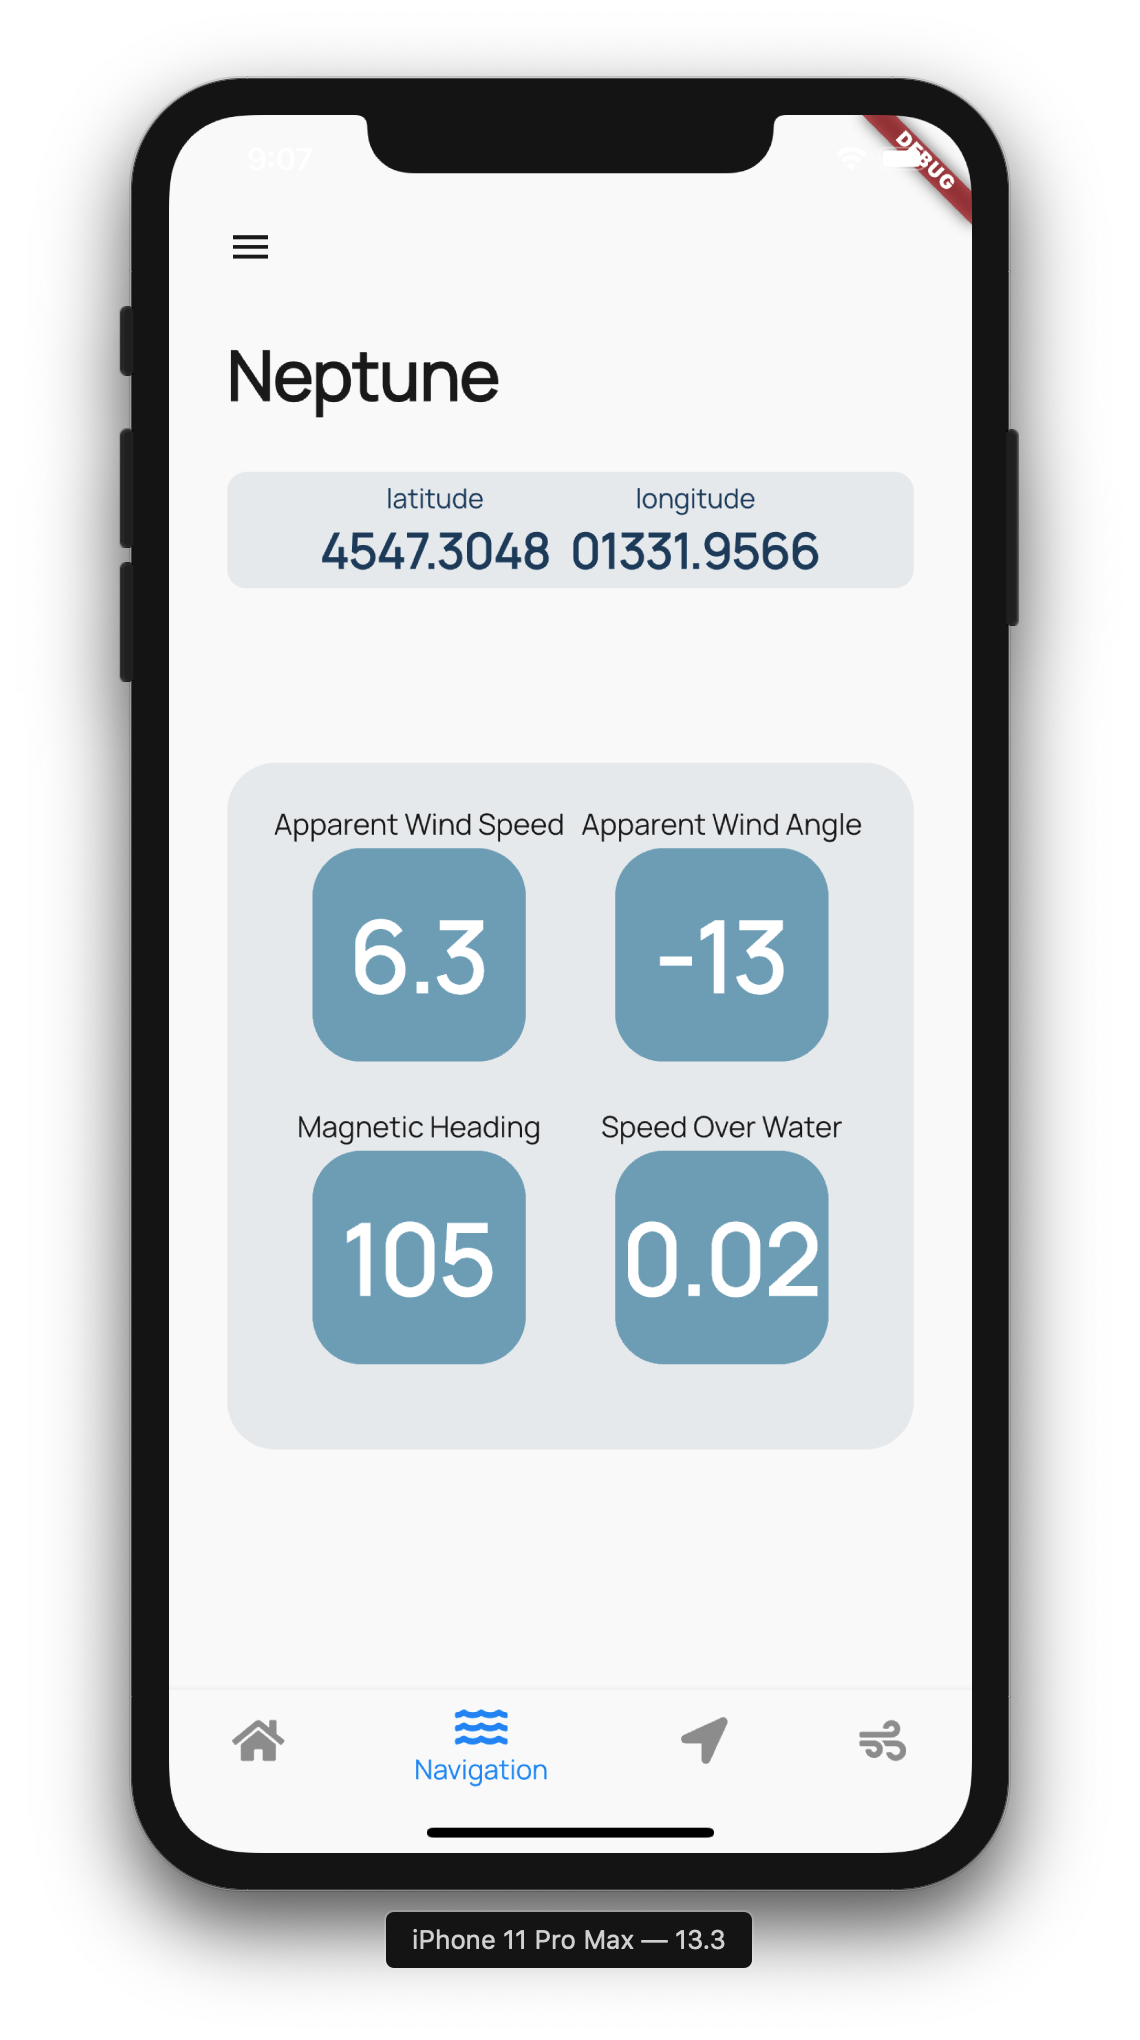
\includegraphics[scale=0.34]{navigation}
		\caption[Screenshot - Navigation]{Screenshot della schermata \textit{Navigation}.}
		\label{figura:navigation}
	\end{center}
\end{figure}

Sulla base dell'architettura proposta (sezione \textit{\nameref{architettura implementata}}), il BLoC relativo alla schermata deve essere posizionato prima dell'oggetto \verb|NavigationPage|. Infatti, nel metodo \verb|create| viene ritornato prima il\\ \verb|Provider<NavigationPage>| e poi, come figlio di quest'ultimo, \verb|NavigationPage|. La schermata viene incapsulata nel \verb|Consumer|: una spiegazione approfondita è stata redatta nella sezione \textit{\nameref{consumer}}.

Nella classe privata \verb|_NavigationPageState| viene utilizzata la \textit{mixin}\\ \verb|AutomaticKeepAliveClientMixin<T>| (un approfondimento è presente nell'appendice \ref{cap:B}), necessario per evitare di ricaricare i dati anche quando si cambia schermata. Il metodo \verb|build()| (dalla riga 37 alla riga 45) ritorna un Widget comune: il \verb|GridBox|. A questo Widget viene passato il corrispondente BLoC, la classe che gestisce i temi e i dati che devono essere visualizzati appena istanziato il Widget. In particolare, \verb|initialData| è necessario nel momento in cui viene avviata l'applicazione e non è stata ancora effettuata alcuna richiesta alla socket. Quindi, non avendo a disposizione dei dati provenienti dal server, il Widget deve comunque illustrare dei dati iniziali. Questi dati iniziali vengono forniti appunto tramite il parametro \verb|initialData|.

\newpage

\subsubsection{GPS e Wind}
\begin{figure}[htp]
	\centering
	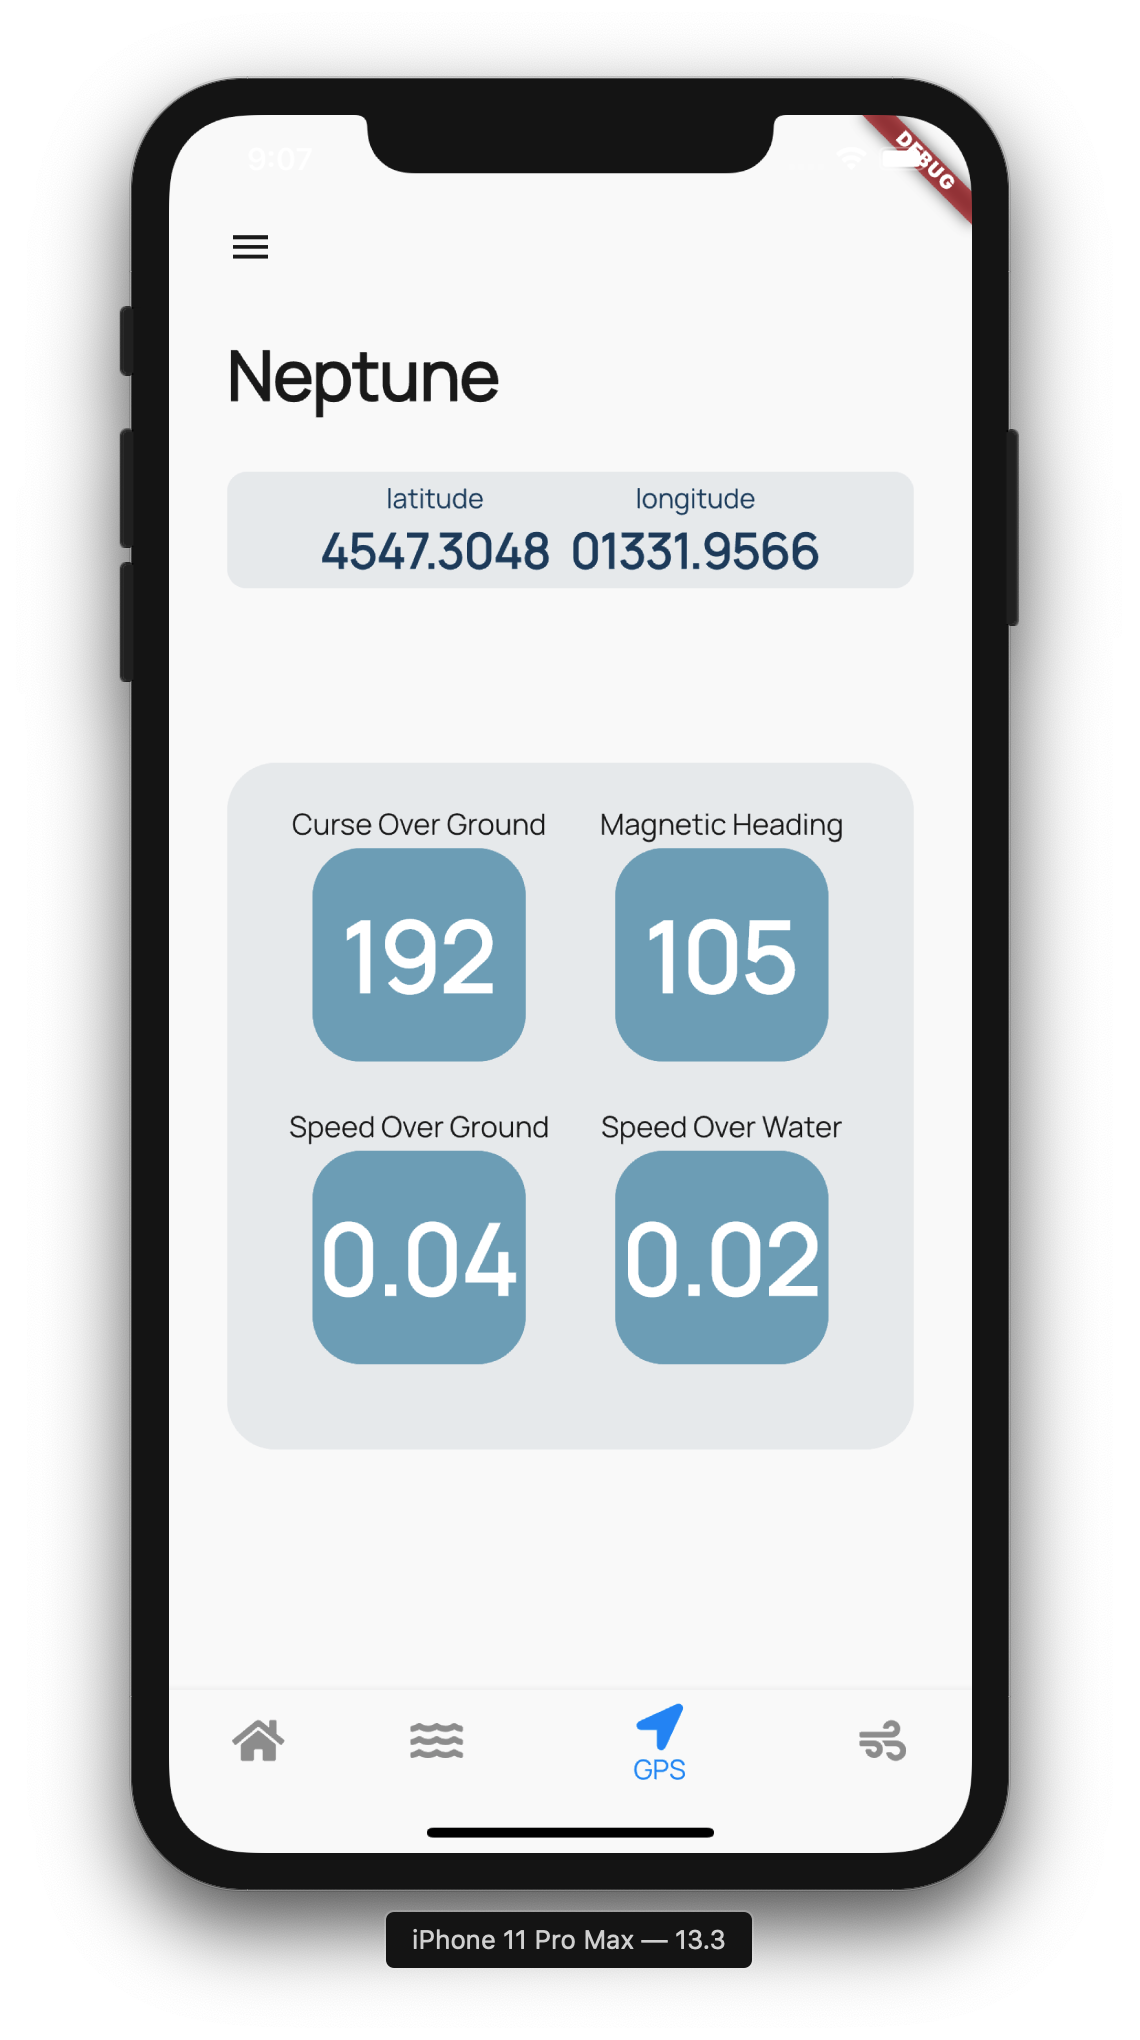
\includegraphics[scale=0.34]{gps}
	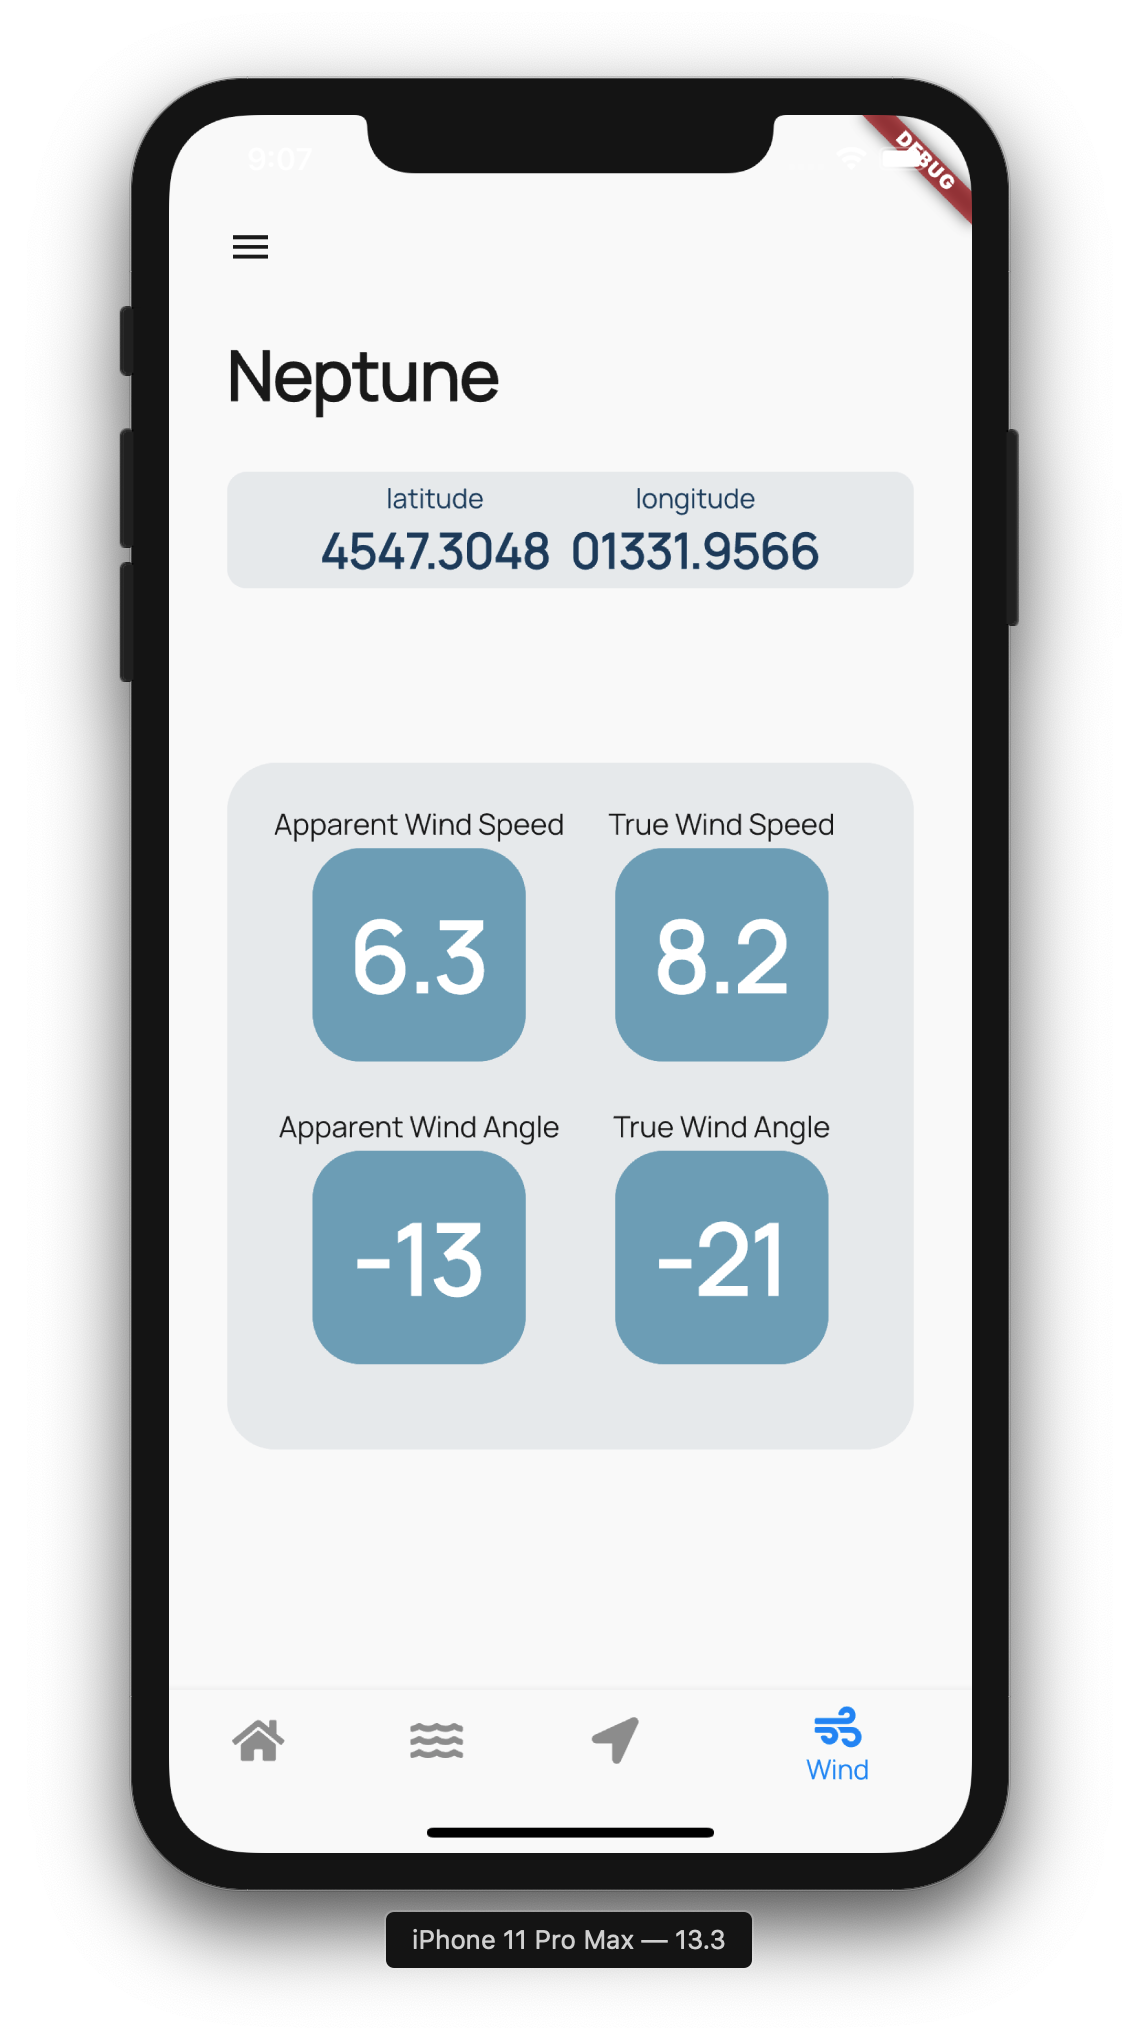
\includegraphics[scale=0.34]{wind}
	\caption[Screenshot - Drawer e della schermata Settings]{Screenshot della schermata \textit{GPS} (a sinistra) e della schermata di \textit{Wind} (a destra).}\label{xyz}
\end{figure}

Nella schermata \textbf{GPS} è possibile monitorare i dati relativi alla geolocalizzazione (le coordinate vengono prese dal sensore GPS installato sul Raspberry e non dal dispositivo in cui viene utilizzata l'applicazione). Mentre, nella schermata \textbf{Wind} è possibile visualizzare i dati relativi al vento, come ad esempio la reale velocità del vento.

In particolare, nella schermata \textit{GPS} è possibile monitorare i seguenti dati:
\begin{enumerate}
	\item \textbf{Curse Over Ground}
	\item \textbf{Magnetic Heading}
	\item \textbf{Speed Over Ground}
	\item \textbf{Speed Over Water}
\end{enumerate}

Nella schermata \textit{Wind} l'utente può controllare i seguenti dati:
\begin{enumerate}
	\item \textbf{Apparent Wind Speed}
	\item \textbf{True Wind Angle}
	\item \textbf{Apparent Wind Angle}
	\item \textbf{True Wind Angle}
\end{enumerate}

La struttura di queste schermate segue il modello semplice e compatto della schermata \textit{Navigation}.

\subsubsection{Dashboard}
Questa è la schermata che l'utente vede all'apertura dell'applicazione. Il principale obiettivo di questa schermata è quello di fornire all'utente un quadro generale della situazione. In questo modo può monitorare tutti i dati riguardanti la navigazione. Inoltre da questa schermata, l'utente può avviare o fermare il \textit{polling} dei dati, ovvero, può avviare o fermare le richieste verso la socket quando lo ritiene opportuno.

Nonostante questa sia la schermata principale dell'applicazione, la spiegazione di essa viene effettuata soltanto ora in quanto possiede una struttura differente rispetto allo schema \textit{standard} delle schermate \textit{Navigation}, \textit{GPS} e \textit{Wind}. Le altre schermate seguono un approccio più semplice: ad ogni pagina è associato un BLoC. Come è possibile notare dal codice della classe \verb|DashboardPage|, non è presente alcun riferimento ad un qualche BLoC. Questa schermata è stata strutturata in modo che la \verb|DashboardPage| possa integrare diversi Widget per comporre una grafica complessiva. Ogni componente grafico al suo interno possiede il proprio BLoC (sia \verb|LocationWidget| che \verb|DashboardWidget|, riga 23 e 24).
\begin{lstlisting}
class DashboardPage extends StatefulWidget {
  DashboardPage({Key key}) : super(key: key);

  @override
  State<StatefulWidget> createState() => _DashboardPageState();
}

class _DashboardPageState extends State<DashboardPage>
    with AutomaticKeepAliveClientMixin<DashboardPage> {
  @override
  bool get wantKeepAlive => true;

  @override
  Widget build(BuildContext context) {
    super.build(context);
    return _buildUI();
  }

  Widget _buildUI() {
    return ListView(
      shrinkWrap: true,
      children: <Widget>[
        LocationWidget.create(context),
        DashboardWidget.create(context),
      ],
    );
  }
}
\end{lstlisting}

Osservando il codice relativo alla classe \verb|DashboardWidget|, è possibile notare che la struttura di  questo componente è sostanzialmente uguale a quella della schermata \textit{Navigation}. Grazie alla pagina \textit{Dashboard}, si possono vedere i benefici e i vantaggi dell'utilizzo di un'architettura BLoC: non è necessario che ogni singola schermata possieda il proprio BLoC, ma possono essere creati dei BLoC per componenti di dimensioni più piccole. Successivamente, questi componenti possono essere assemblati in un unico Widget, come nel caso della \textit{Dashboard} con i Widget \textit{Location} e \textit{DashboardWidget}.

\begin{lstlisting}
class DashboardWidget extends StatefulWidget {
  DashboardWidget(
      {Key key, @required this.dashboardBloc, 
      @required this.themeHandler})
      : super(key: key);
  final DashboardWidgetBloc dashboardBloc;
  final ThemeHandler themeHandler;

  static Widget create(BuildContext context) {
    final RepositorySocket repository =
        Provider.of<RepositorySocket>(context, listen: false);

    final ThemeHandler themeHandler =
        Provider.of<ThemeHandler>(context, listen: false);

    return Provider<DashboardWidgetBloc>(
      create: (_) => DashboardWidgetBloc(
          repository: repository, 
          socketData: repository.socketData),
      dispose: (context, bloc) => bloc.dispose(),
      child: Consumer<DashboardWidgetBloc>(
          builder: (context, bloc, _) =>
              DashboardWidget(dashboardBloc: bloc, 
              themeHandler: themeHandler)),);
  }

  @override
  State<StatefulWidget> createState() => _DashboardWidgetState();
}

class _DashboardWidgetState extends State<DashboardWidget>
    with AutomaticKeepAliveClientMixin<DashboardWidget> {
  @override
  bool get wantKeepAlive => true;

  @override
  Widget build(BuildContext context) {
    super.build(context);
    return StreamBuilder<Dashboard>(
      stream: widget.dashboardBloc.stream,
      initialData: Dashboard(),
      builder: (context, snapshot) {
        return _buildGrid(snapshot.data.toMap());
      },
    );
  }

  Widget _buildGrid(Map<String, dynamic> dashboardData) { ... }

  Widget _buildButtons() { ... }

  Widget _buildSingleBox(Map<String, dynamic> dashboardData, 
  String key) { ... }
}
\end{lstlisting}

\begin{figure}[htp]
	\centering
	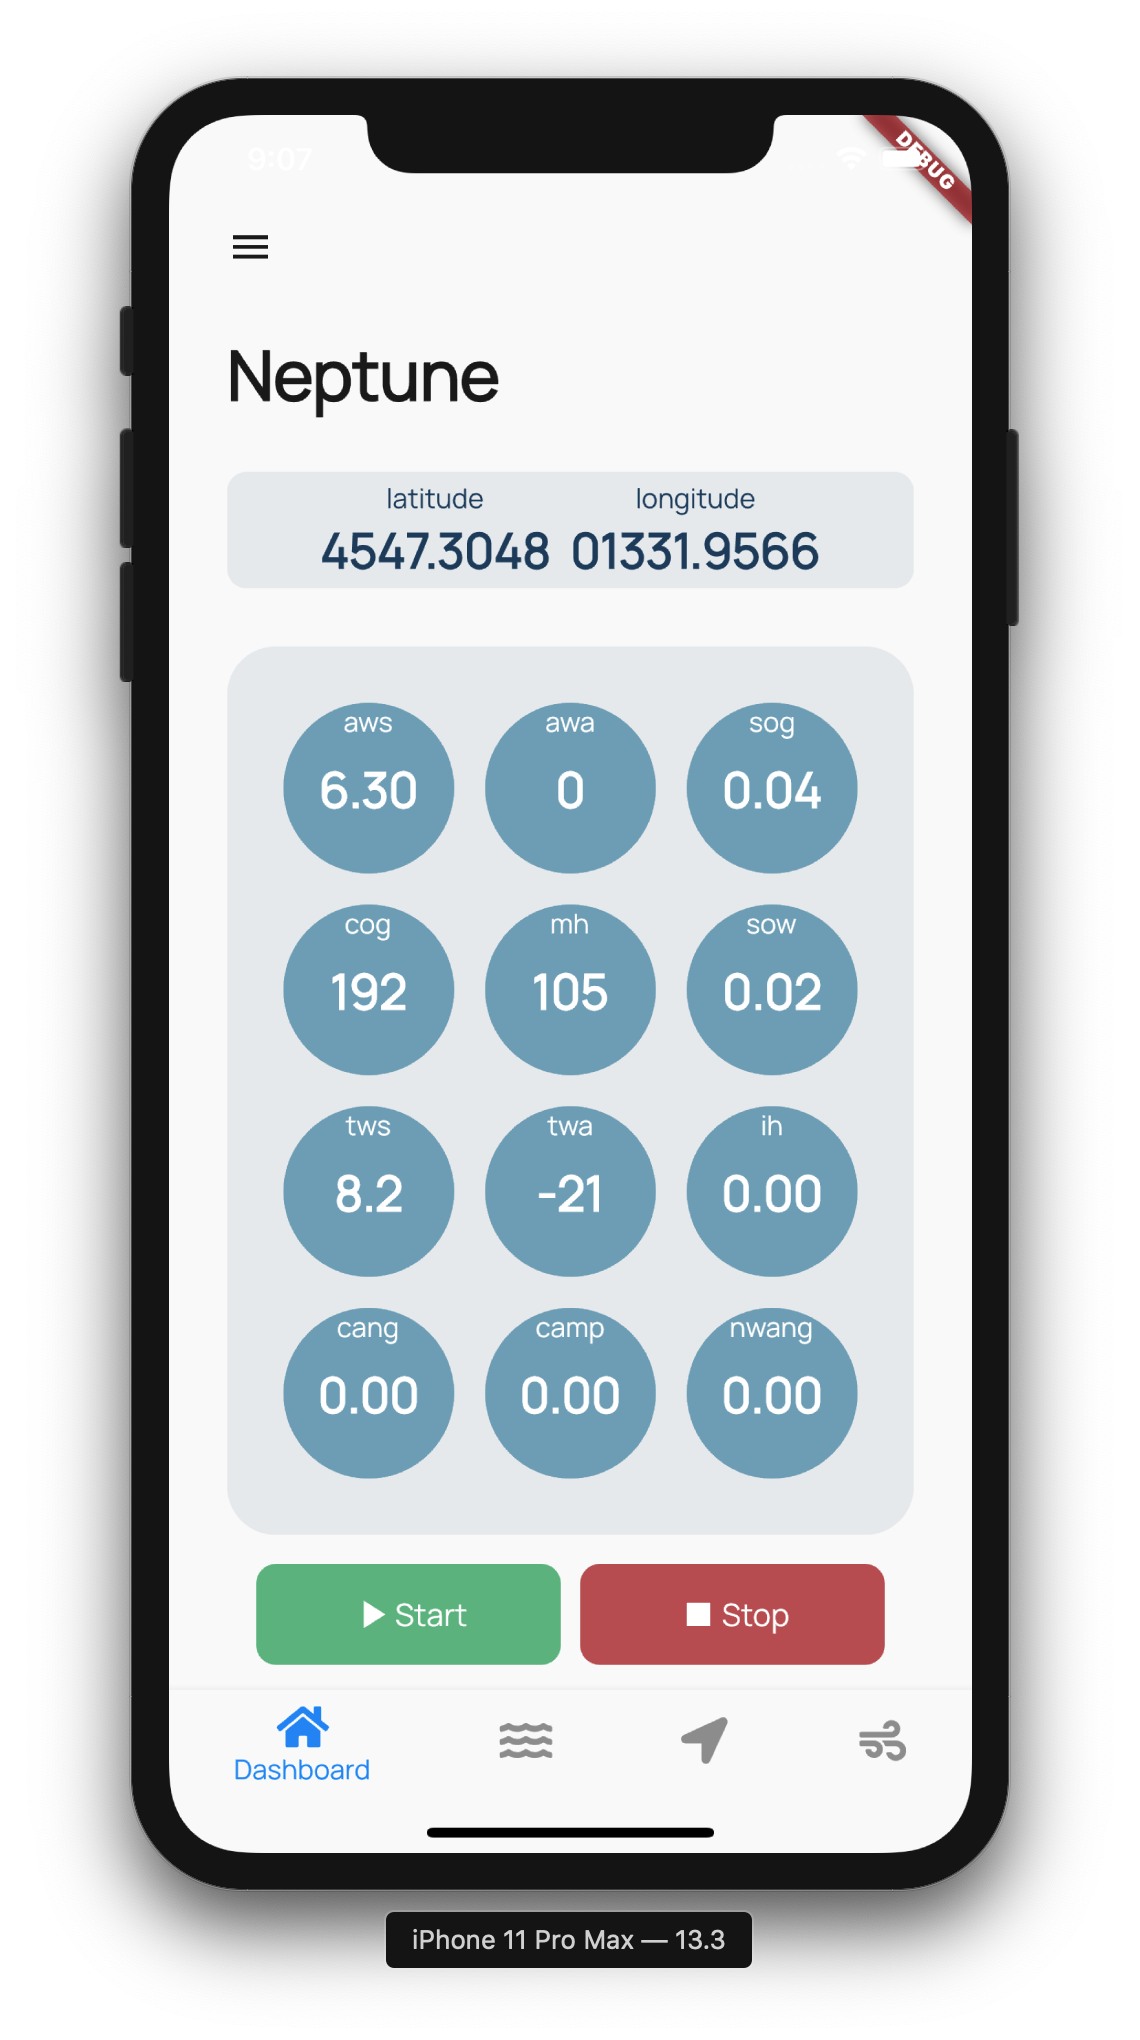
\includegraphics[scale=0.35]{dashboard}
	\caption[Screenshot - Dashboard]{Screenshot della schermata \textit{Dashboard}.}\label{xyz}
\end{figure}

\newpage

\subsubsection{Settings}
Questa schermata presenta una lista delle varie impostazioni che possono essere modificate dall'utente. In questa versione dell'applicazione, possiamo notare tre opzioni:
\begin{enumerate}
	\item \textbf{Cache}
	\item \textbf{Server}
	\item \textbf{Theme}
\end{enumerate}

Facendo \textit{tap} su una di queste opzioni, l'utente verrà portato sulla schermata corrispondente. Per accedere alla schermata delle impostazioni, si deve accedere al \textit{drawer}, posto in alto a sinistra dell'applicazione.

Di seguito viene presentato il codice di questa schermata. È possibile notare la mappa \verb|options| (dalla riga 10 alla riga 29) che va a creare delle associazioni tra il nome della schermata, in formato stringa, e l'oggetto che deve essere istanziato nel caso in cui l'utente faccia tap su una di queste opzioni.

Dal codice è possibile notare inoltre la facilità dell'utilizzo dei Widget: nel metodo \verb|build| è presente il Widget \verb|ListView.builder|, il quale permette di iterare su un oggetto \textit{enumerabile}, come ad esempio delle liste. All'interno di tale Widget, viene utilizzato \verb|ListTile|, un componente grafico che permette di realizzare le voci presenti nella schermata \textit{Settings} (Figura 6.10, screenshot a destra). Tutto questo è possibile realizzarlo con poche righe di codice, sfruttando pochi Widget.

\begin{lstlisting}
class SettingsPage extends StatefulWidget {
  final String title = "Settings";

  @override
  State<StatefulWidget> createState() => _SettingsPageState();
}

class _SettingsPageState extends State<SettingsPage>
    with AutomaticKeepAliveClientMixin<SettingsPage> {
  final Map<String, dynamic> options = {
    "cache": {
      "title": Text("Cache"),
      "leading": Icon(Icons.cached),
      "subtitle": Text("Delete the data saved from the app"),
      "page": CachePage(),
    },
    "server": {
      "title": Text("Server"),
      "leading": Icon(Icons.perm_data_setting),
      "subtitle": Text("Choose the server to connect to"),
      "page": ServerPage(),
    },
    "theme": {
      "title": Text("Theme"),
      "leading": Icon(Icons.color_lens),
      "subtitle": Text("Choose the theme of the app"),
      "page": ThemePage(),
    },
  };

  StatefulWidget _getSettingPage(String option) {
    return options[option]["page"];
  }

  @override
  Widget build(BuildContext context) {
    super.build(context);
    return Scaffold(
      appBar: PageAppBar(context: context, title: widget.title),
      body: ListView.builder(
        itemCount: options.length,
        itemBuilder: (ctx, i) {
          return Padding(
            padding: const EdgeInsets.only(
              left: 20.0,
              right: 20.0,
              bottom: 25.0,
            ),
            child: Container(
              decoration: BoxDecoration(
                color: ColorsPalette.softGrey,
                borderRadius: BorderRadius.circular(10.0),
              ),
              child: ListTile(
                leading: options[
                options.keys.toList()[i]]["leading"],
                title: options[
                options.keys.toList()[i]]["title"],
                subtitle: options[
                options.keys.toList()[i]]["subtitle"],
                trailing: Icon(CupertinoIcons.forward),
                onTap: () async {
                  Future<Widget> buildPageAsync() async {
                    return Future.microtask(() {
                      return _getSettingPage(
                      options.keys.toList()[i]);
                    });
                  }

                  Widget page = await buildPageAsync();
                  MaterialPageRoute route =
                      MaterialPageRoute(builder: (_) => page);
                  Navigator.push(context, route);
                },
              ),
            ),
          );
        },
      ),
    );
  }

  @override
  bool get wantKeepAlive => true;
}
\end{lstlisting}

\begin{figure}[htp]
	\centering
	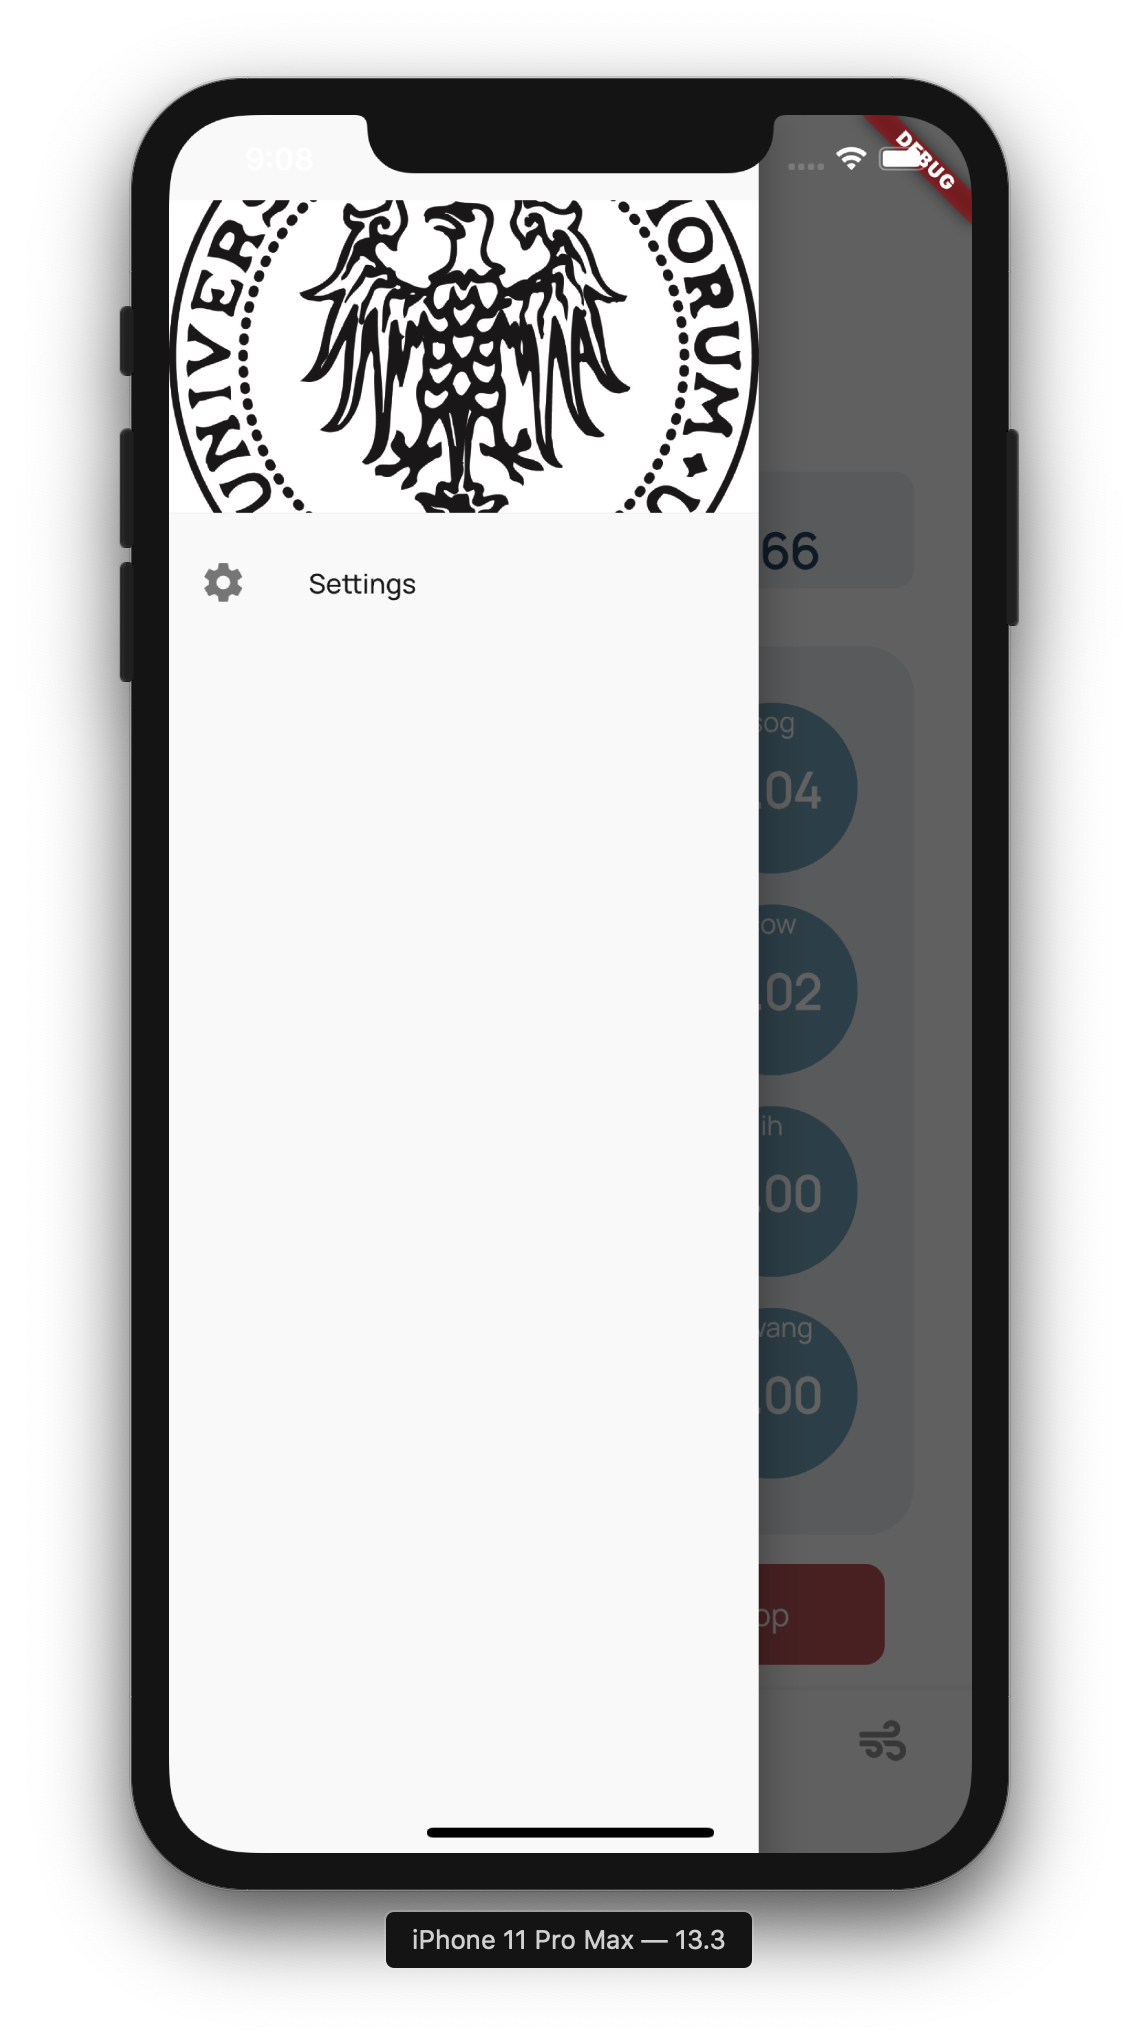
\includegraphics[scale=0.34]{drawer}
	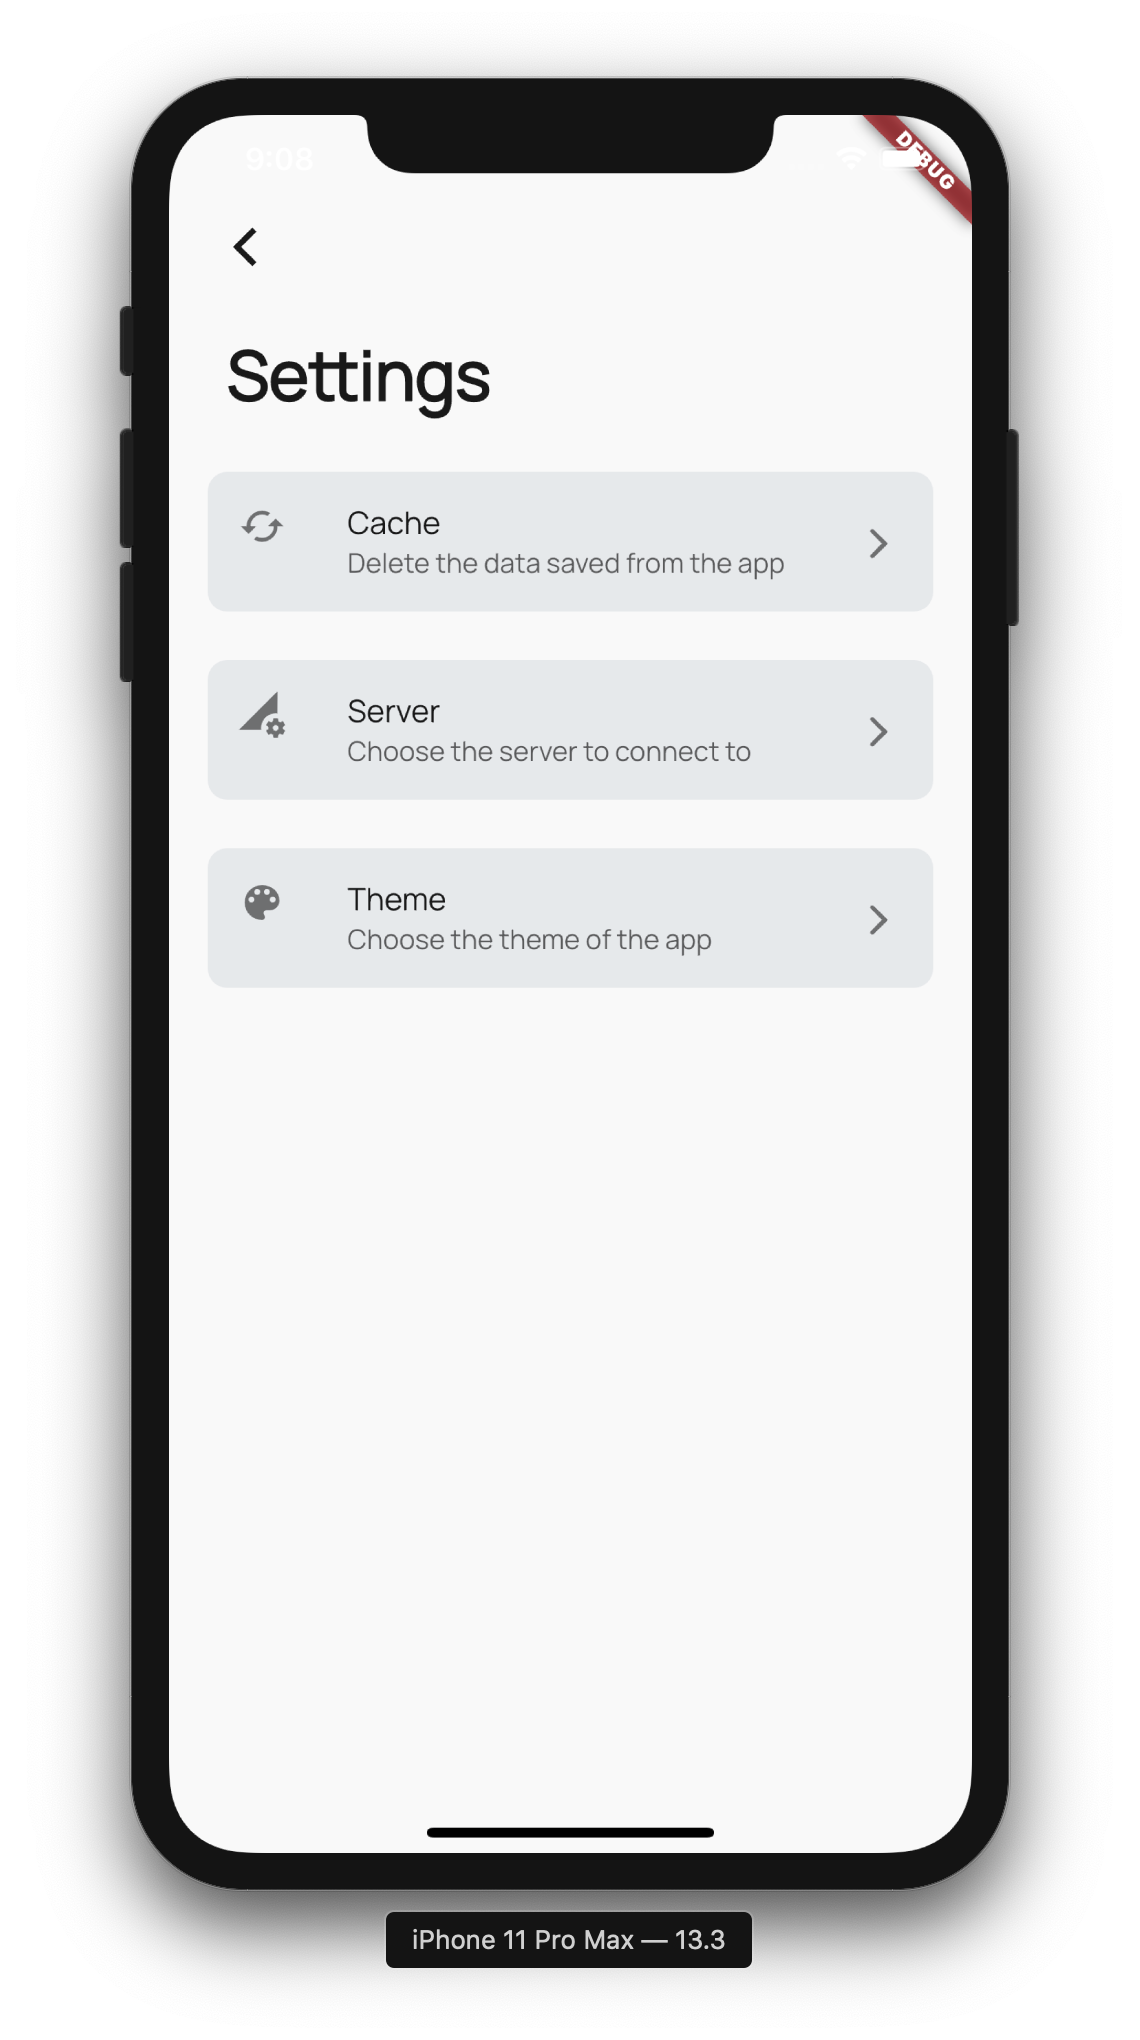
\includegraphics[scale=0.34]{settings}
	\caption[Screenshot - Drawer e della schermata Settings]{Screenshot del \textit{drawer} dell'applicazione (a sinistra) e della schermata di \textit{Settings} (a destra).}\label{xyz}
\end{figure}

\newpage

\subsubsection{Cache}
In questa schermata l'utente può eliminare i dati salvati nella \textit{cache}. Facendo un \textit{tap} sull'unica voce presente nella schermata (Figura 6.11), si presenterà un \textit{Alert Dialog} per chiedere la conferma della pulizia della cache. Se la cache è vuota, anche se si volesse selezionare la voce, non comparirà alcuna Alert Dialog.

\begin{figure}
	\begin{center}
		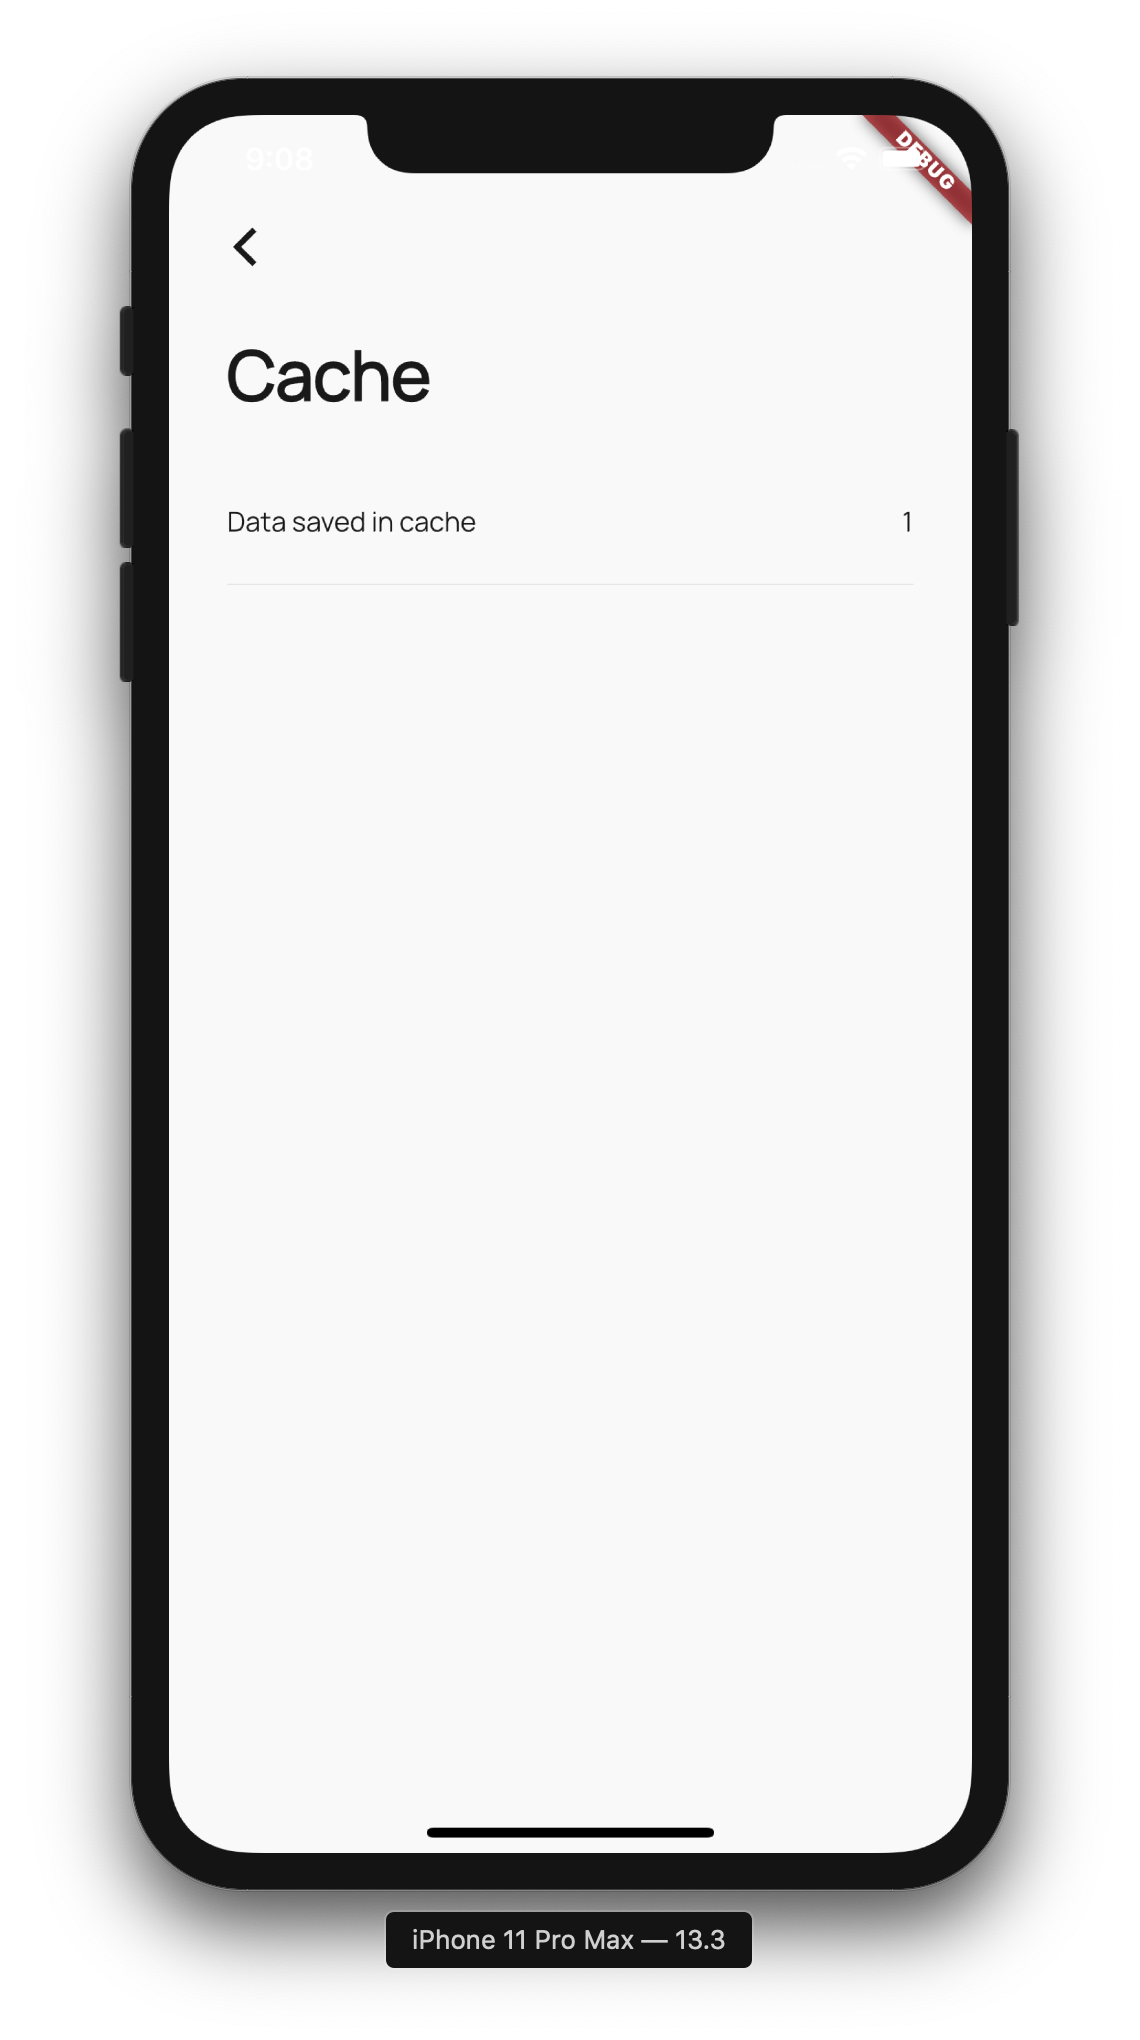
\includegraphics[scale=0.34]{cache}
		\caption[Screenshot - Cache]{Screenshot della schermata \textit{Cache}.}
		\label{figura:cache}
	\end{center}
\end{figure}

Dagli screenshot in Figura 6.12, è possibile notare che sono state riprodotte le Alert Dialog sia per i dispositivi con sistema operativo Android che iOS. Le diverse Alert Dialog sono fornite direttamente da Flutter.

\begin{figure}[htp]
	\centering
	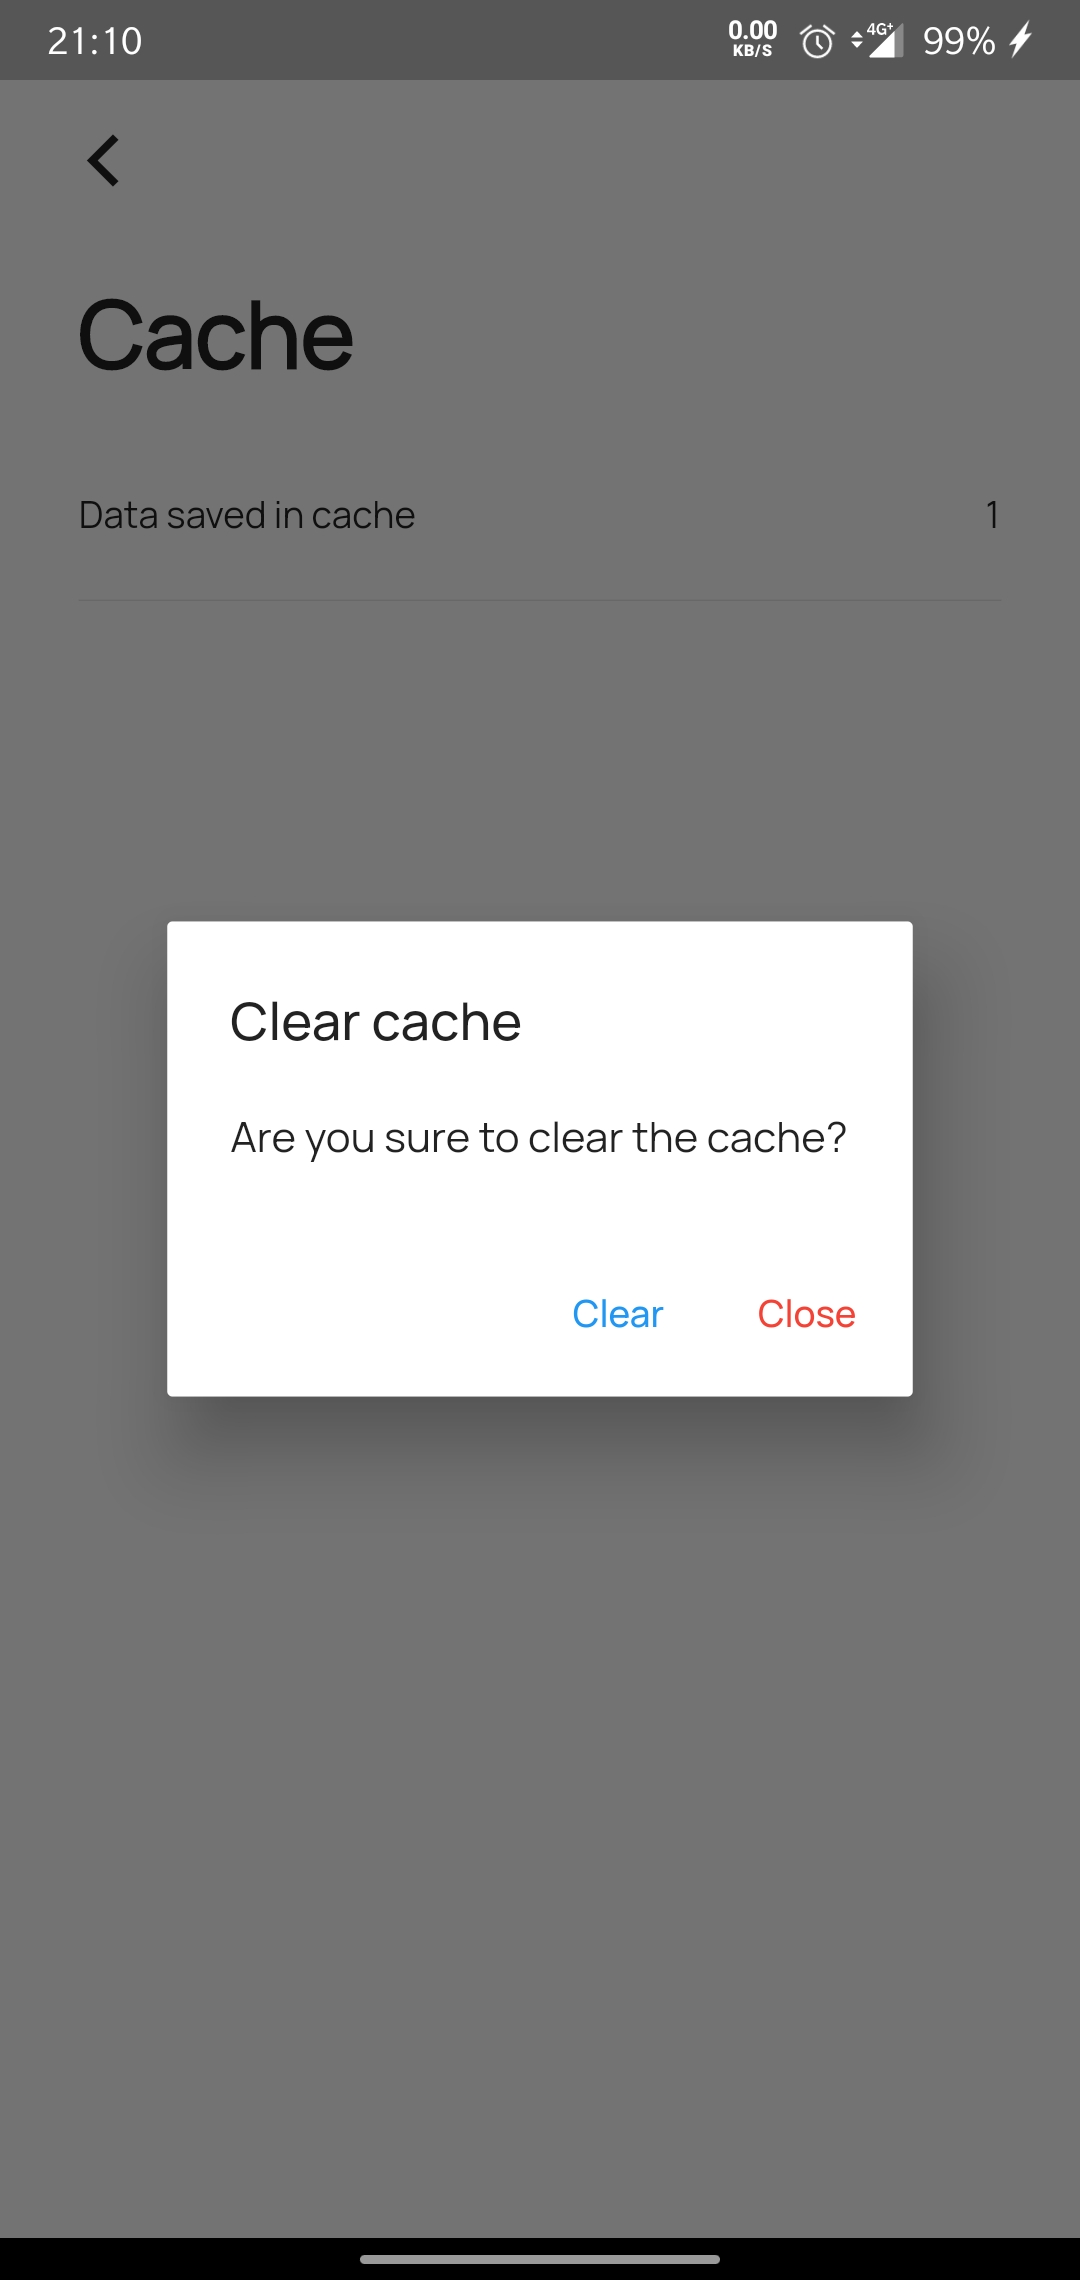
\includegraphics[scale=0.15]{cache_android_dialog}
	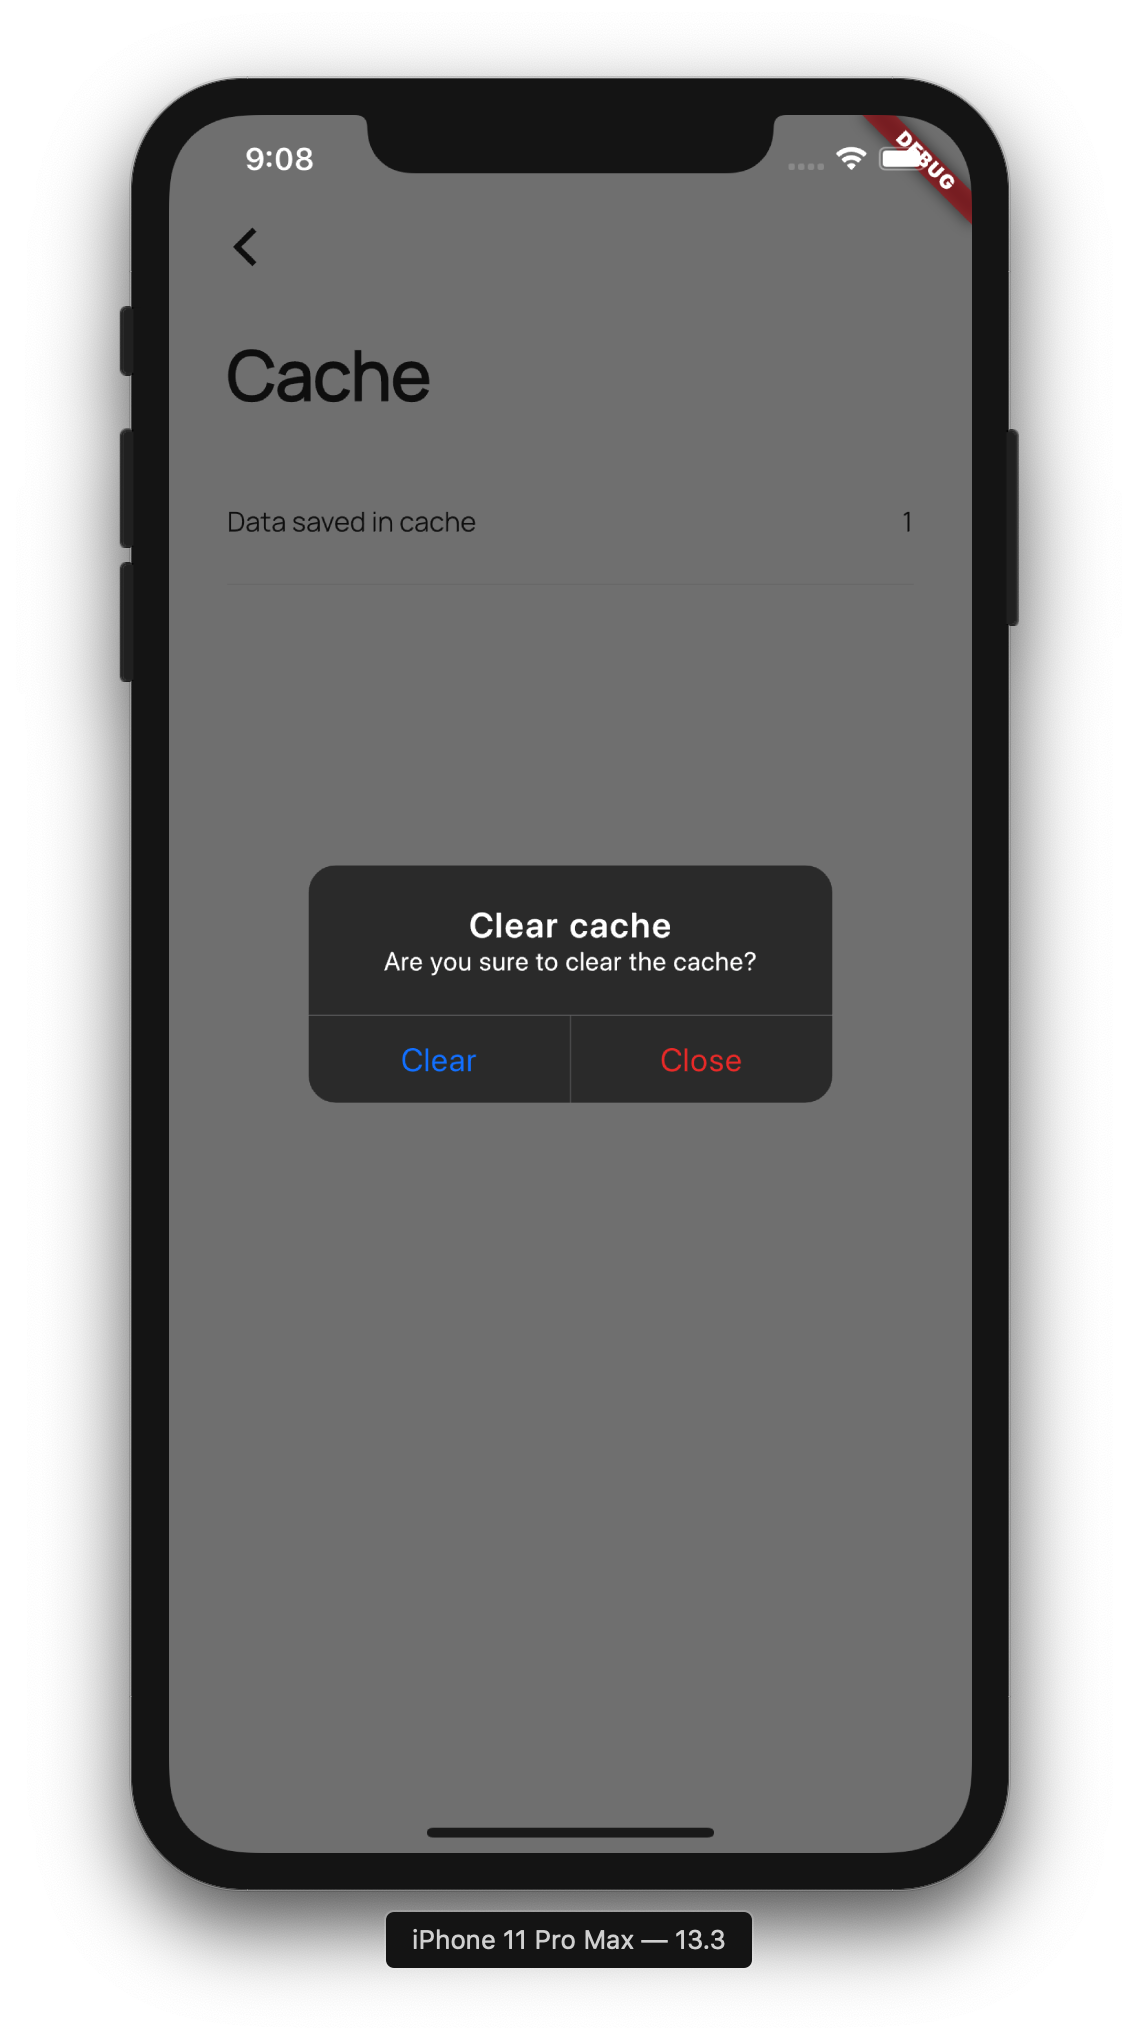
\includegraphics[scale=0.35]{cache_ios_dialog}
	\caption[Screenshot - Alert Dialog in Android e iOS della schermata Cache]{Screenshot dell'\textit{Alert Dialog} per dispositivi Android (a sinistra) e iOS (a destra).}\label{xyz}
\end{figure}

\newpage

\subsubsection{Server}
Questa schermata offre due principali funzionalità:
\begin{enumerate}
	\item Controllo dello stato della \textit{connessione};
	\item Modifica dei parametri per la connessione al server e per il \textit{polling}.
\end{enumerate}

\begin{figure}
	\begin{center}
		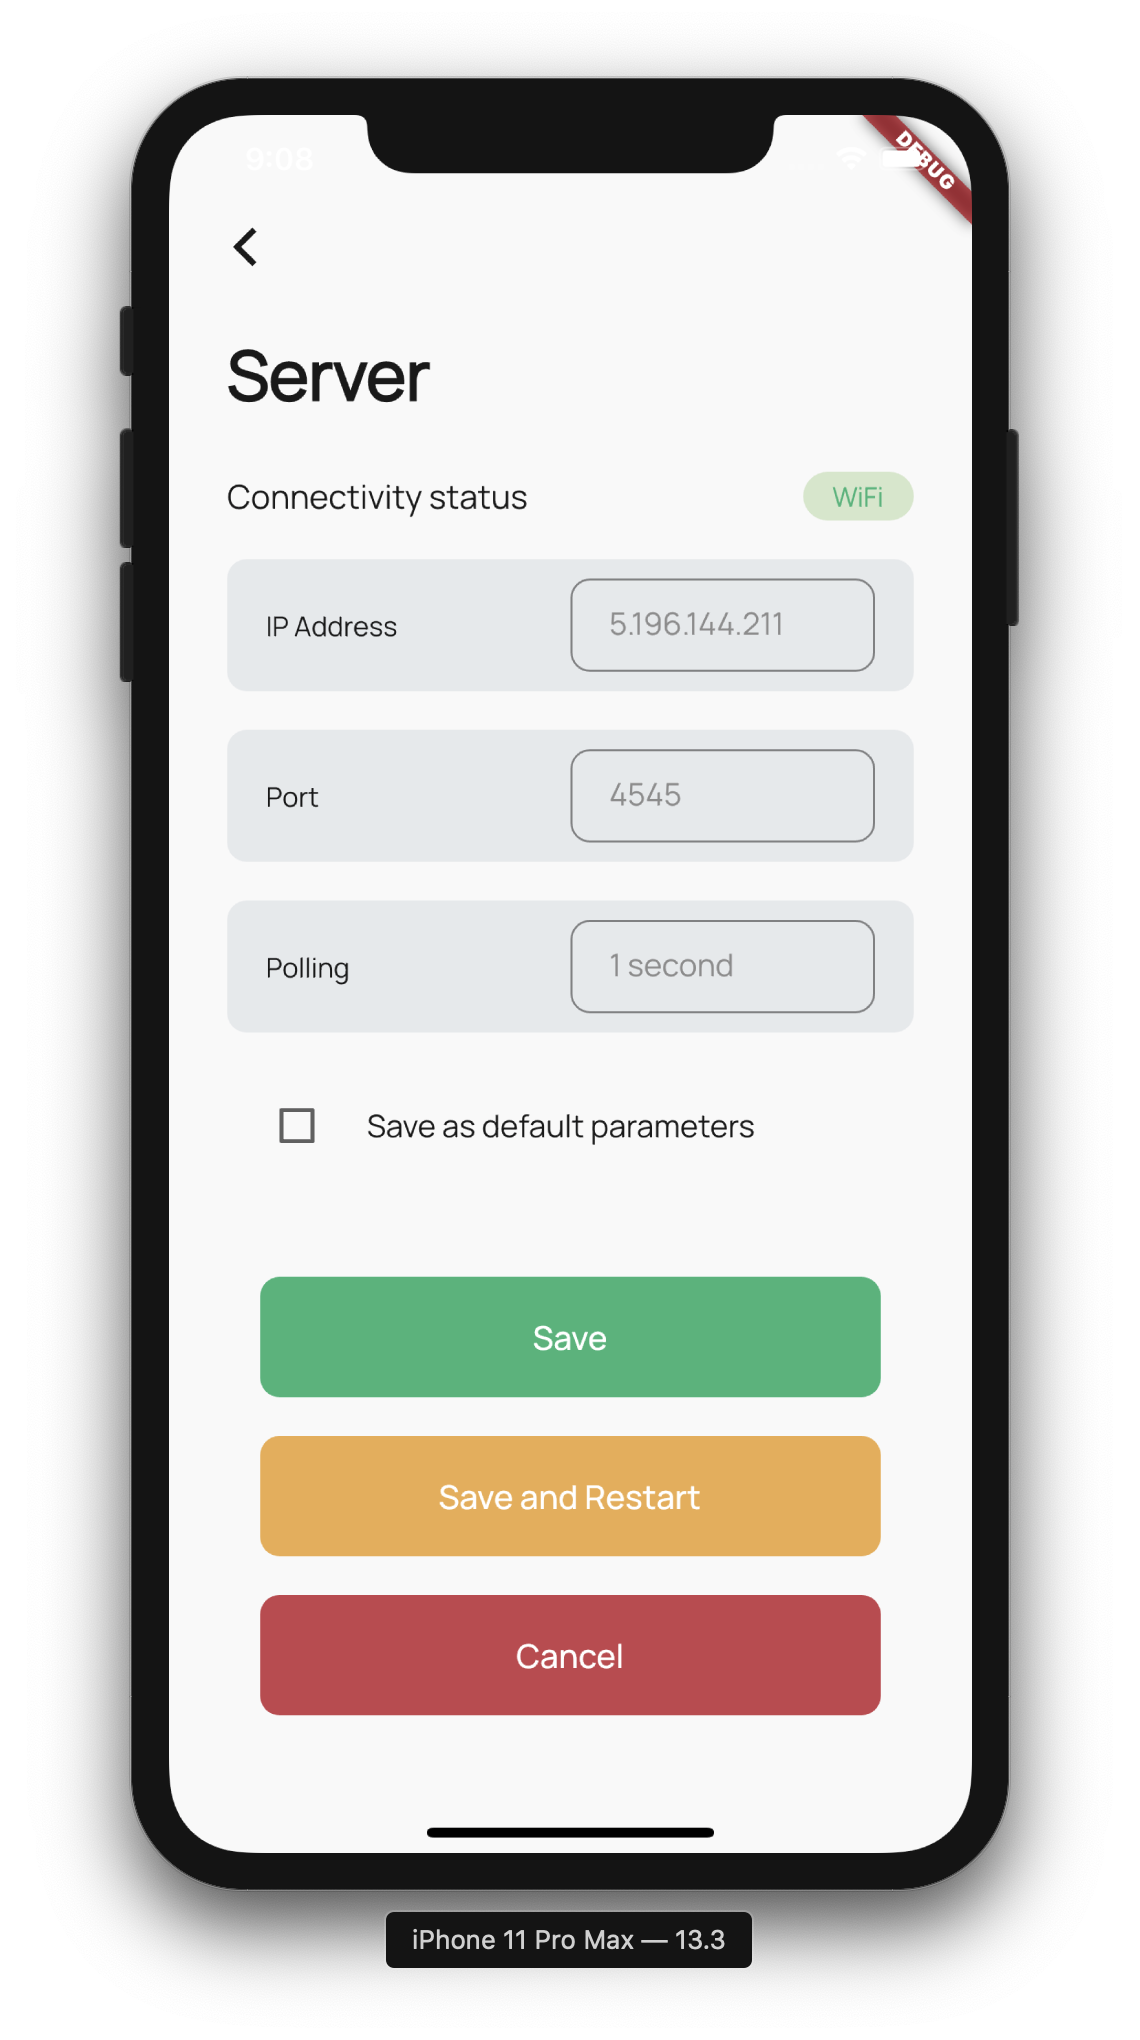
\includegraphics[scale=0.34]{server}
		\caption[Screenshot - Server]{Screenshot della schermata \textit{Server}.}
		\label{figura:server}
	\end{center}
\end{figure}

Per quanto riguarda la prima funzionalità, quando viene rilevato un cambio di stato della connessione, ad esempio da una rete \textit{WiFi} ad una rete \textit{mobile}, questo viene reso noto dalla componente grafica evidenziata negli screenshot presenti nella Figura 6.14. Nel caso in cui sia assente la connessione ad Internet, viene mostrata la dicitura "\textit{offline}". Questa funzionalità è stata possibile implementarla grazie all'utilizzo di un particolare plugin che offre il team di Flutter: \verb|connectivity| (l'applicazione si basa sulla versione \verb|0.4.8+2| del plugin) \cite{connectivity_plugin}. Questo pacchetto fornisce una serie di metodi che permettono di controllare lo stato della connessione.

\begin{figure}[htp]
	\centering
	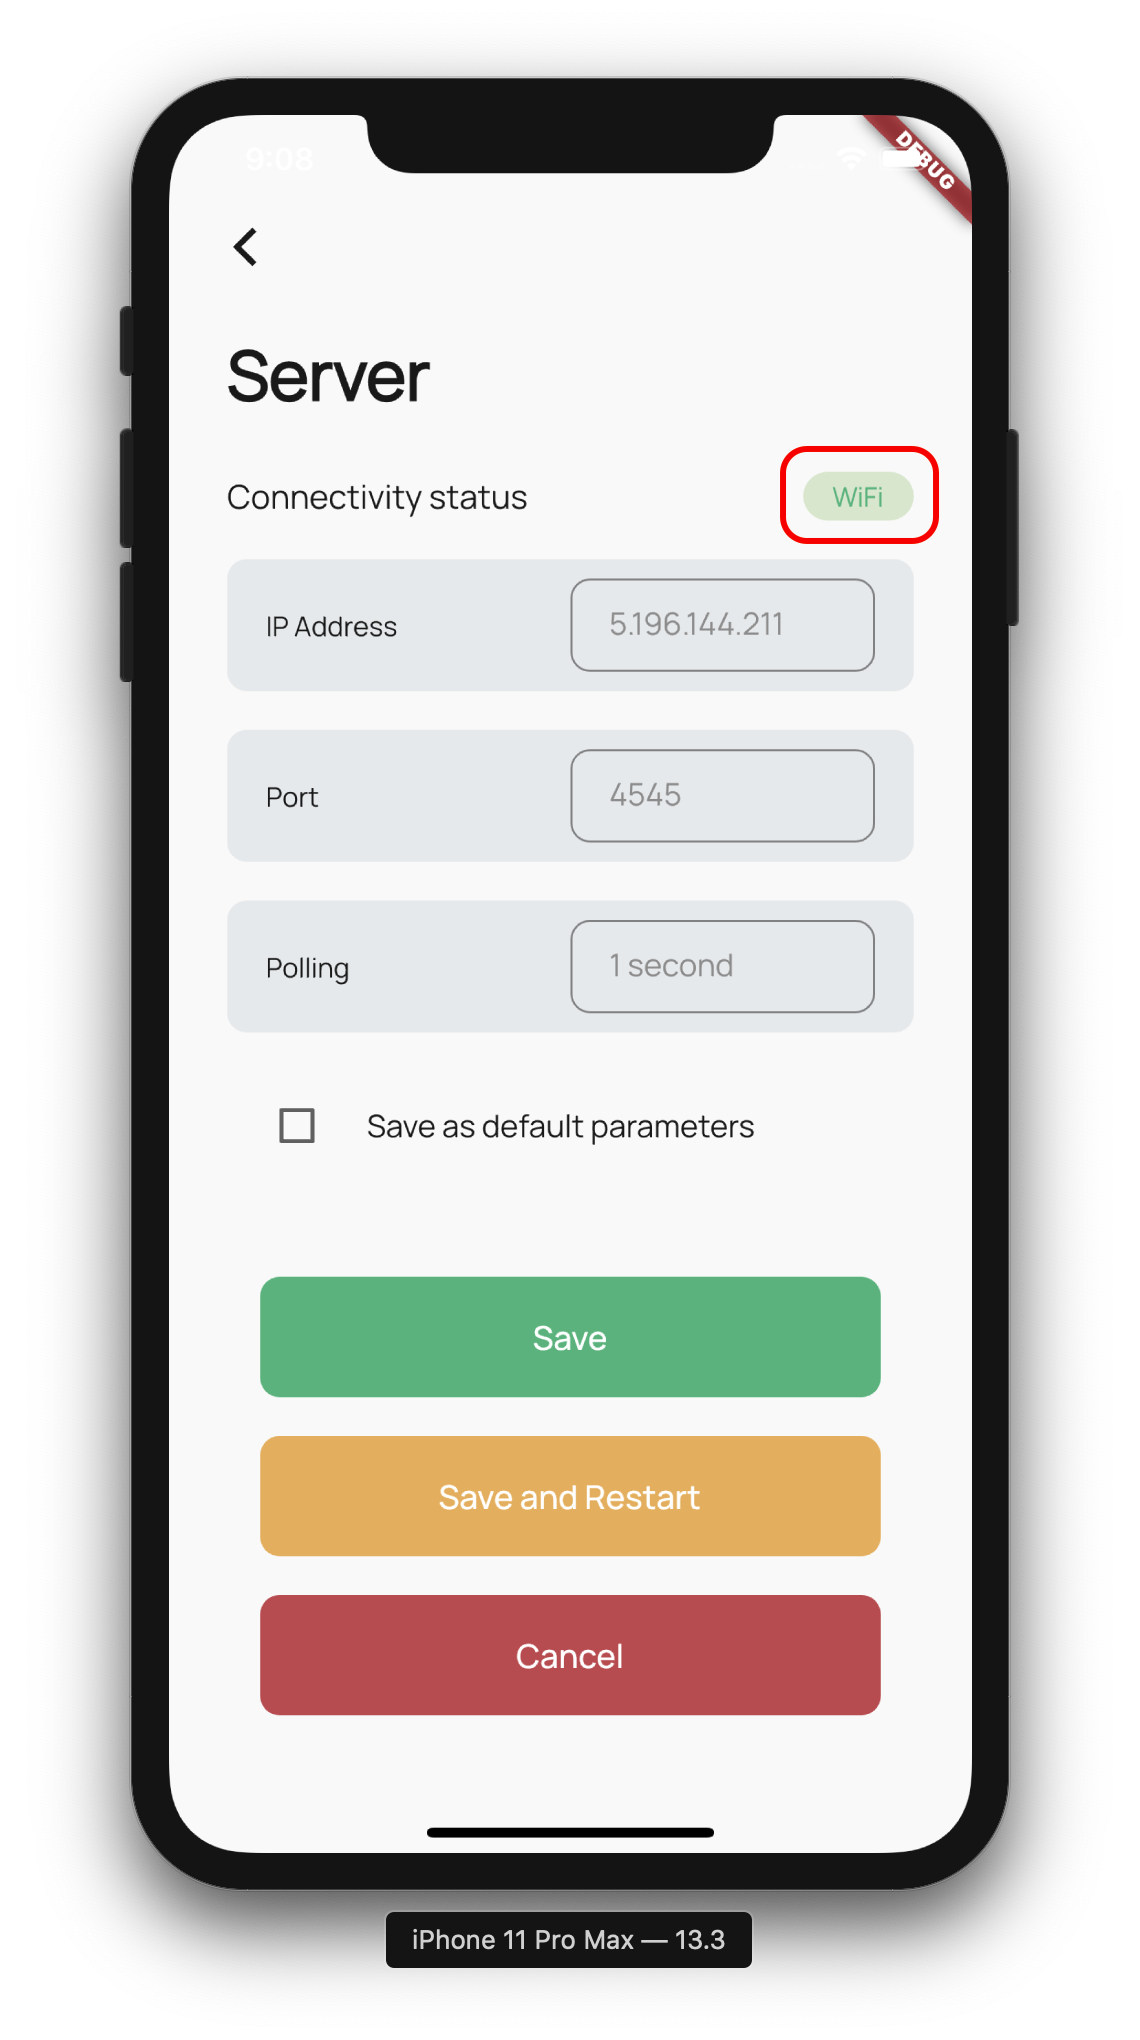
\includegraphics[scale=0.34]{server_online_status}
	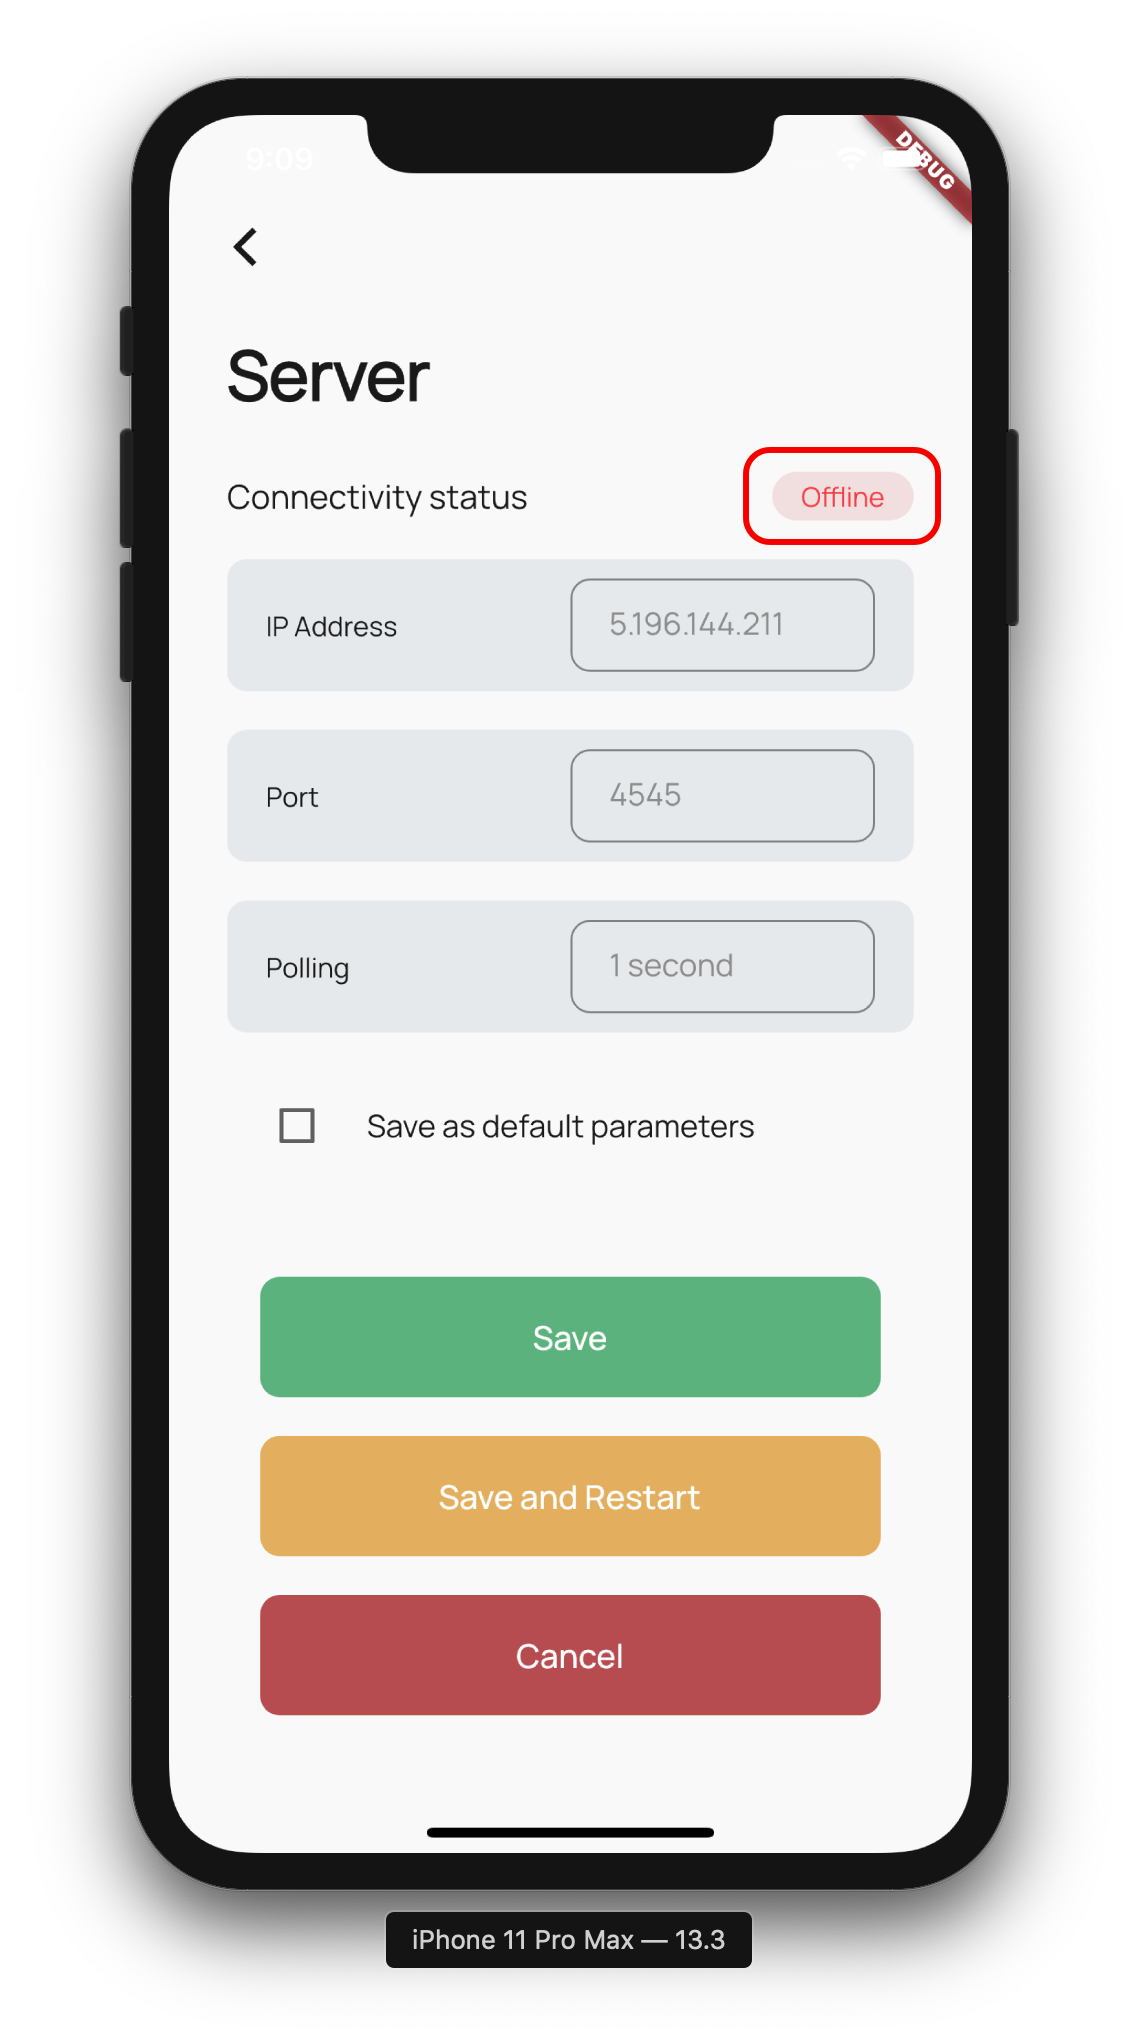
\includegraphics[scale=0.34]{server_offline_status}
	\caption[Screenshot - Controllo dello stato della connessione nella schermata Server]{Tramite un apposito ascoltatore ed il pacchetto (\textit{connectivity 0.4.8+2} \cite{connectivity_plugin}), l'utente può verificare lo stato della connessione Internet.}\label{xyz}
\end{figure}

Dalla riga 8 fino alla riga 15, viene inizializzato un ascoltatore che appena rileva un cambio di stato della connessione, aggiorna lo stato dell'applicazione (nel metodo \verb|setState(() {})|). In questo pezzo di codice, viene sfruttata appieno la \textit{programmazione reattiva}: appena il contenuto della variabile privata \verb|_connectivityStatus| cambia, questo viene propagato nell'albero dei Widget, senza dover eseguire ulteriori istruzioni. 

\newpage

\begin{lstlisting}
...

@override
  void initState() {
    super.initState();
    getInitialStatus();

    _subscription = Connectivity()
        .onConnectivityChanged
        .listen((ConnectivityResult result) {
      setState(() {
        _connectivityStatus = getTextStatus(result);
      });
    });
  }

  void getInitialStatus() async {
    var connectivityResult = await (
    Connectivity().checkConnectivity());
    setState(() {
      _connectivityStatus = getTextStatus(connectivityResult);
    });
    
...
\end{lstlisting}

Per quanto riguarda la funzionalità di modifica dei parametri, quando i dati inseriti rispettano i formati e i vincoli richiesti, è possibile notare nella parte inferiore dell'applicazione una \textit{SnackBar}. Lo scopo della \textit{SnackBar} è quello di notificare l'utente che i dati sono stati inseriti correttamente e che l'aggiornamento dei nuovi parametri inseriti è avvenuto con successo (Figura 6.15). Nel caso in cui invece l'utente abbia inserito dei dati non corretti dal punto di vista del formato o dei vincoli imposti, viene visualizzata una \textit{Alert Dialog} (Figura 6.16). Se vengono generati più errori in un'unica richiesta, questi verranno mostrati tutti insieme in una sola \textit{Alert Dialog}.
\begin{figure}
	\begin{center}
		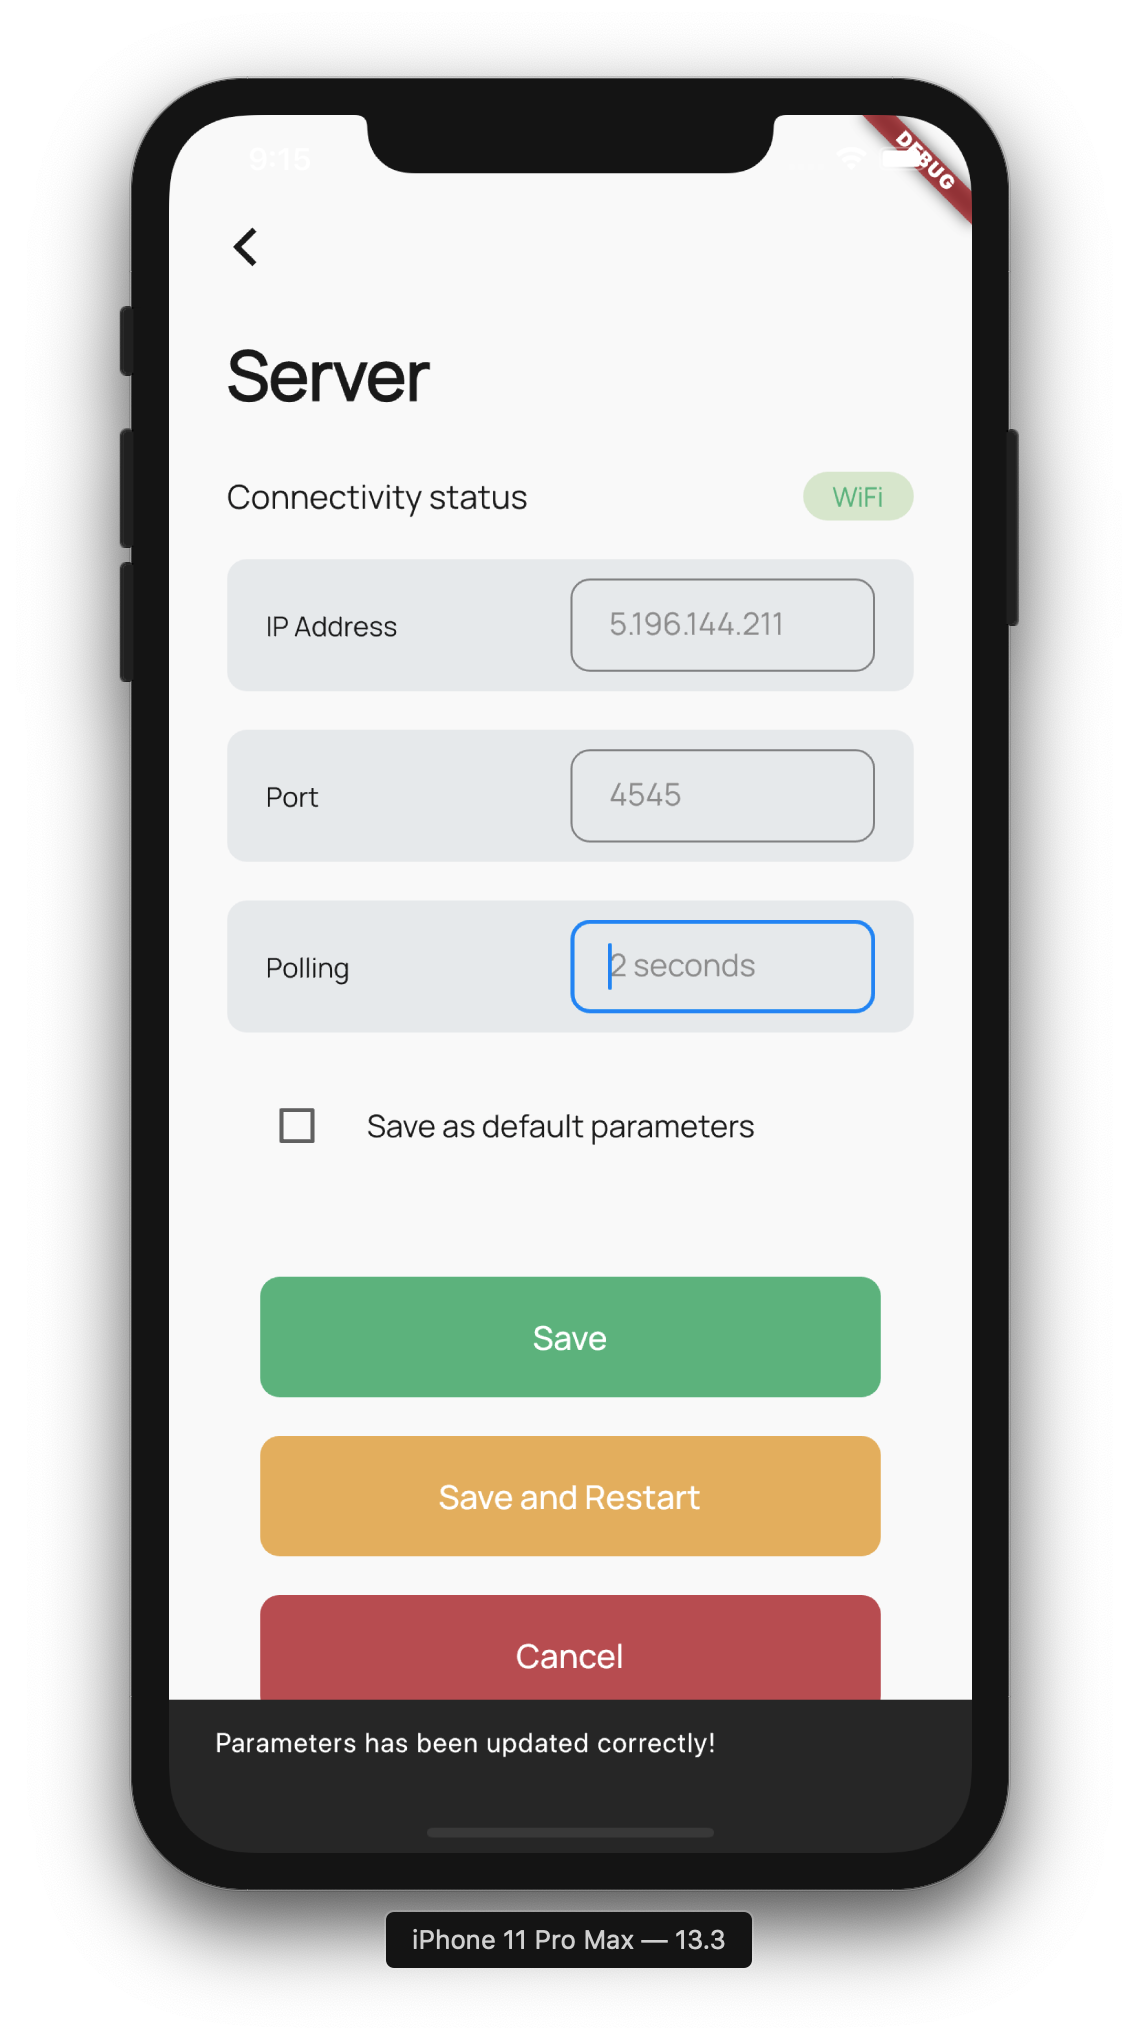
\includegraphics[scale=0.34]{server_successful}
		\caption[Screenshot - Salvataggio dei dati con successo nella schermata Server]{È possibile notare la \textit{SnackBar} che notifica che i dati sono stati inseriti correttamente e che sono stati aggiornati.}
		\label{figura:server_successful}
	\end{center}
\end{figure}

\begin{figure}[htp]
	\centering
	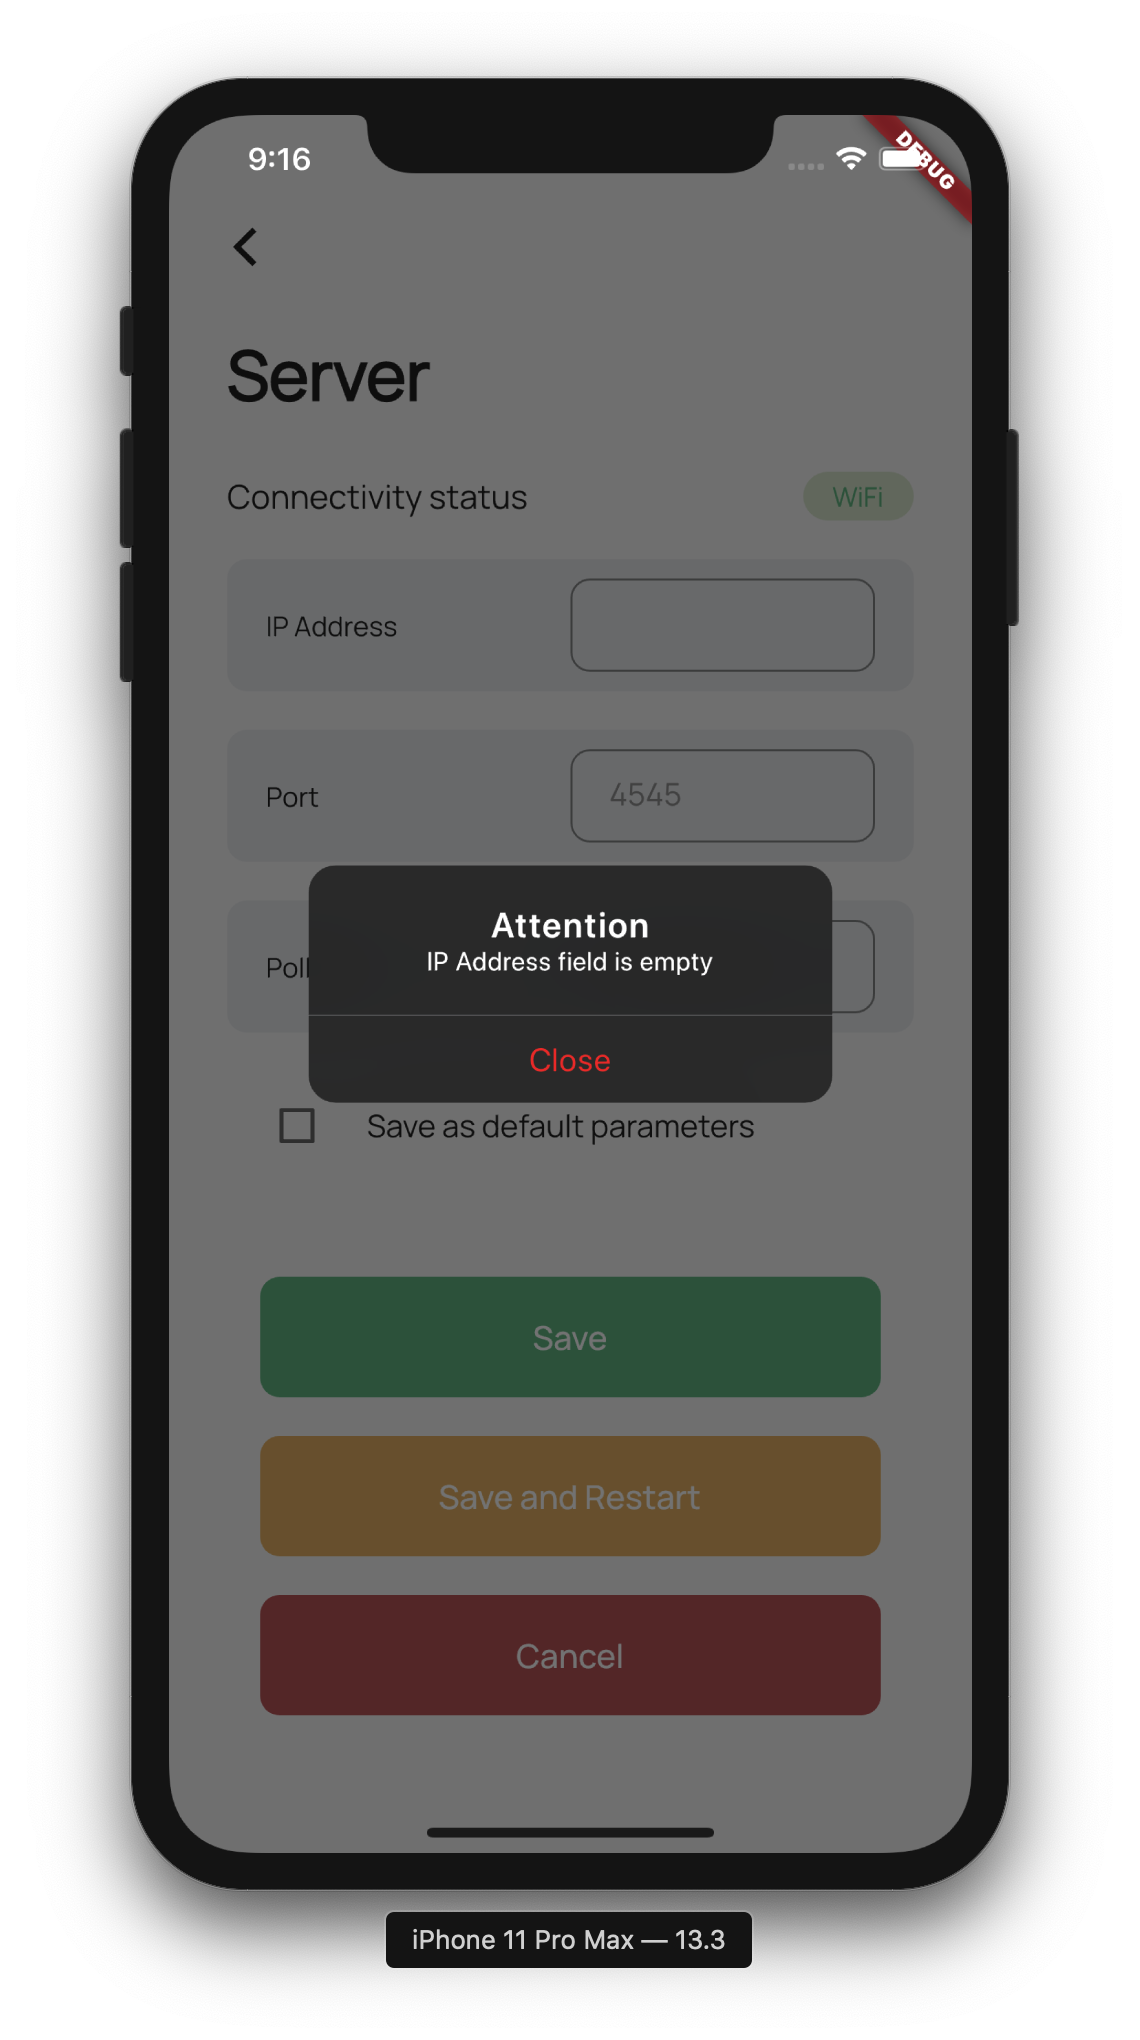
\includegraphics[scale=0.34]{server_error}
	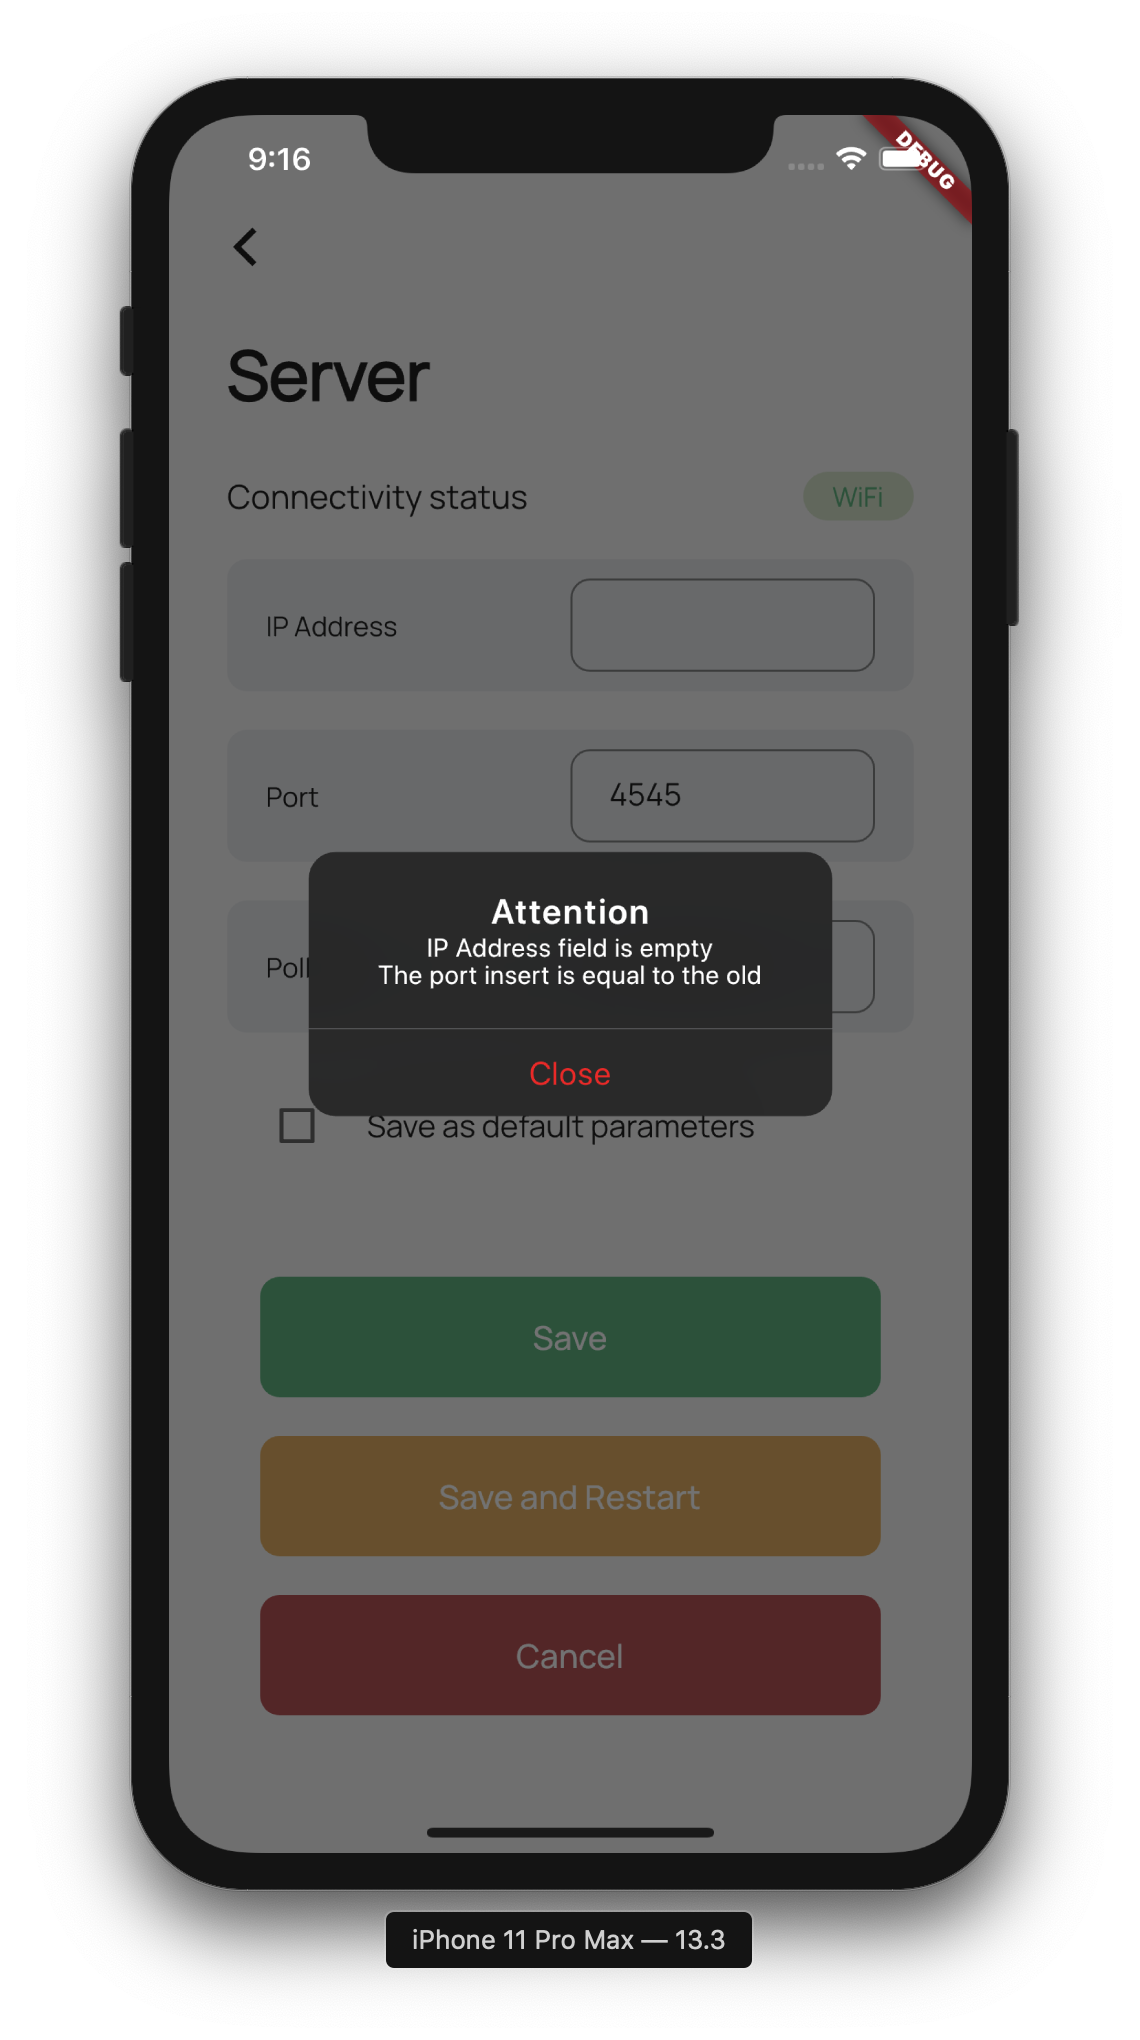
\includegraphics[scale=0.34]{server_errors}
	\caption[Screenshot - Alert Dialog di errore nella schermata Server]{Quando vengono inseriti dei parametri in un formato non accettato, viene visualizzata una \textit{Alert Dialog}.}\label{xyz}
\end{figure}

\newpage

\subsubsection{Temi}
In questa schermata, l'utente può selezionare uno dei temi forniti dall'applicazione. In questa versione dell'app sono presenti soltanto due temi: \textit{default} e ad \textit{alto contrasto}.
È possibile attivare o disattivare l'attivazione del tema ad \textit{alto contrasto} tramite l'apposito \textit{switch} (Widget \verb|Switch|). Quando il tema viene attivato o disattivato, anche il testo dell'opzione cambia. Osservando la Figura 6.17, nella schermata di sinistra il tema ad \textit{alto contrasto} è attivato, mentre a destra è disattivato.

\begin{figure}[htp]
	\centering
	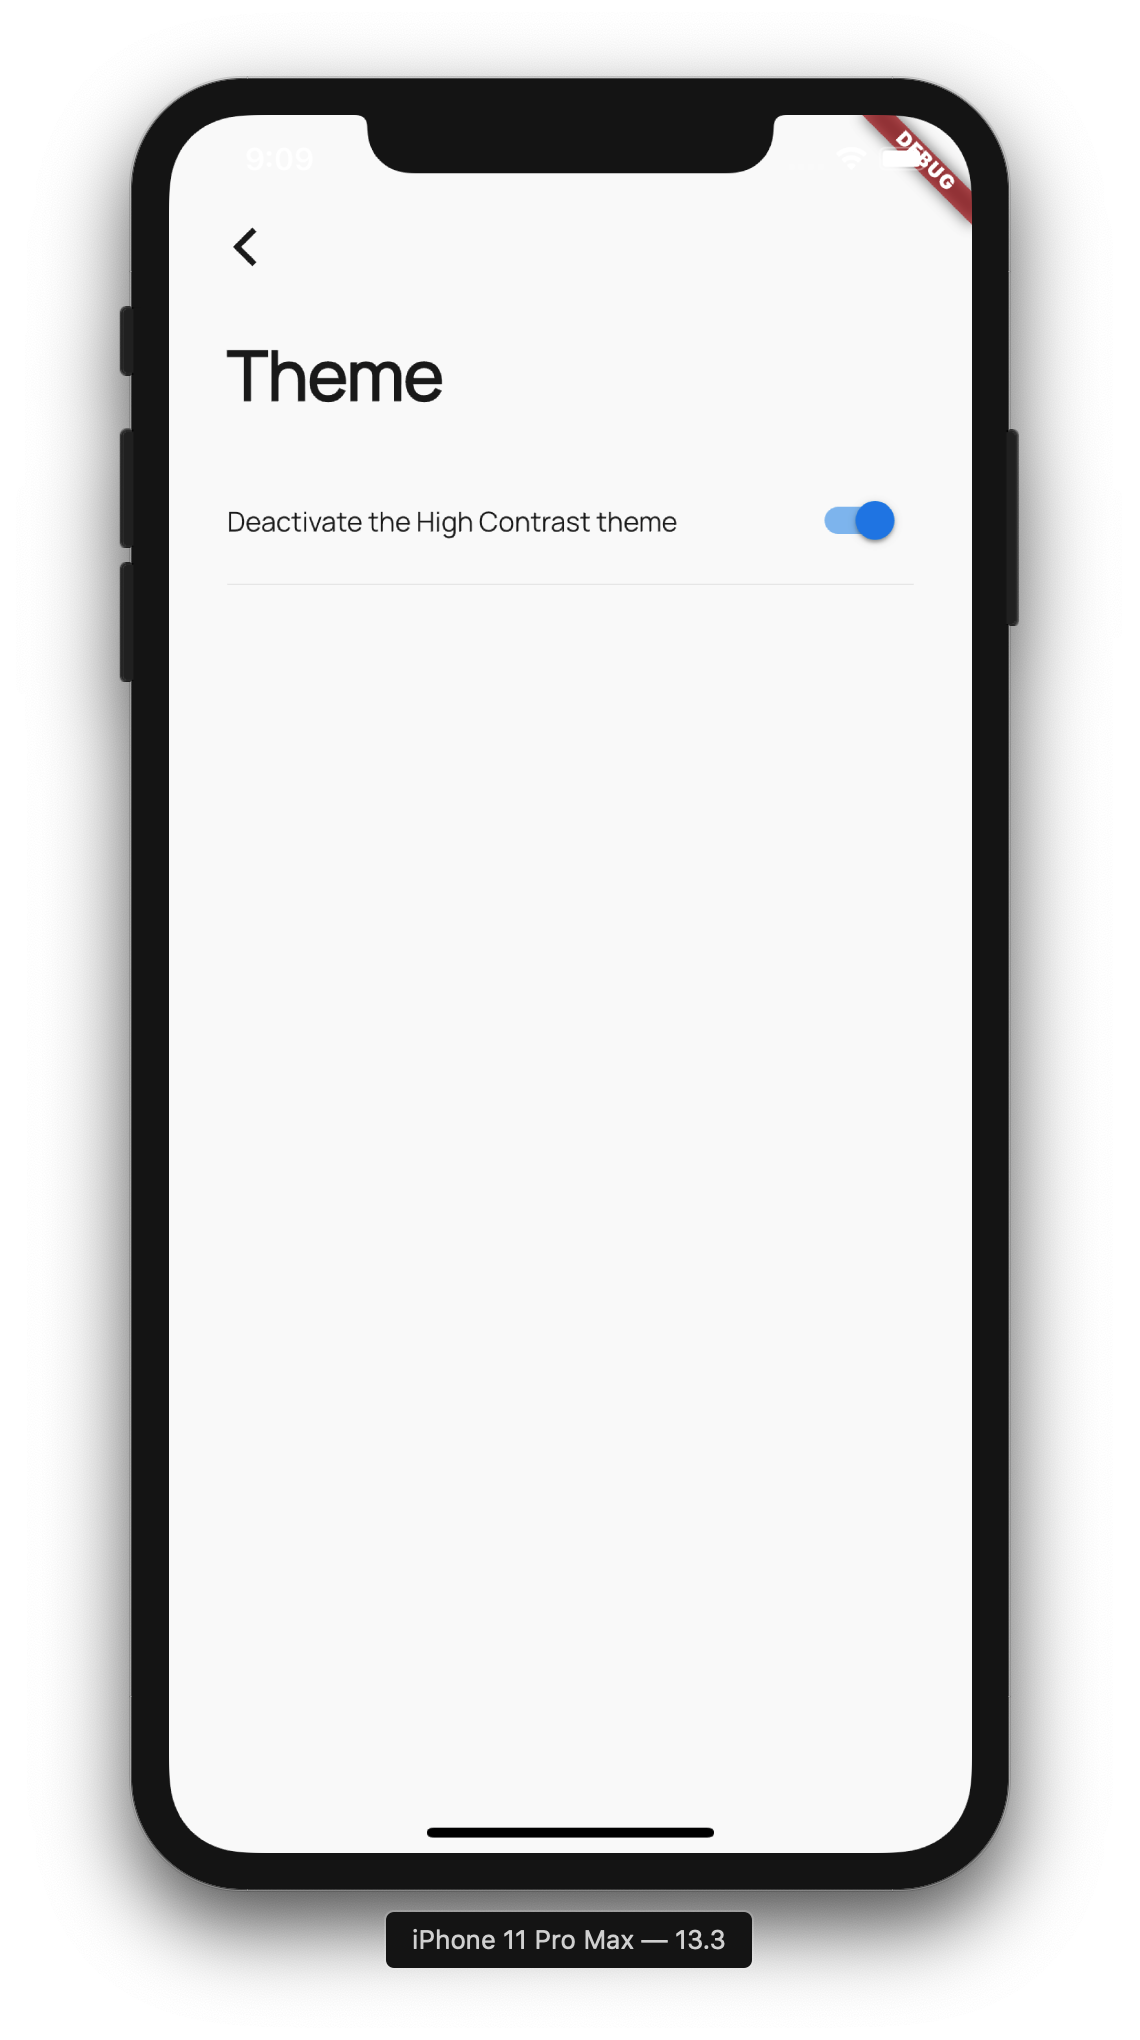
\includegraphics[scale=0.34]{theme_high_contrast_activate}
	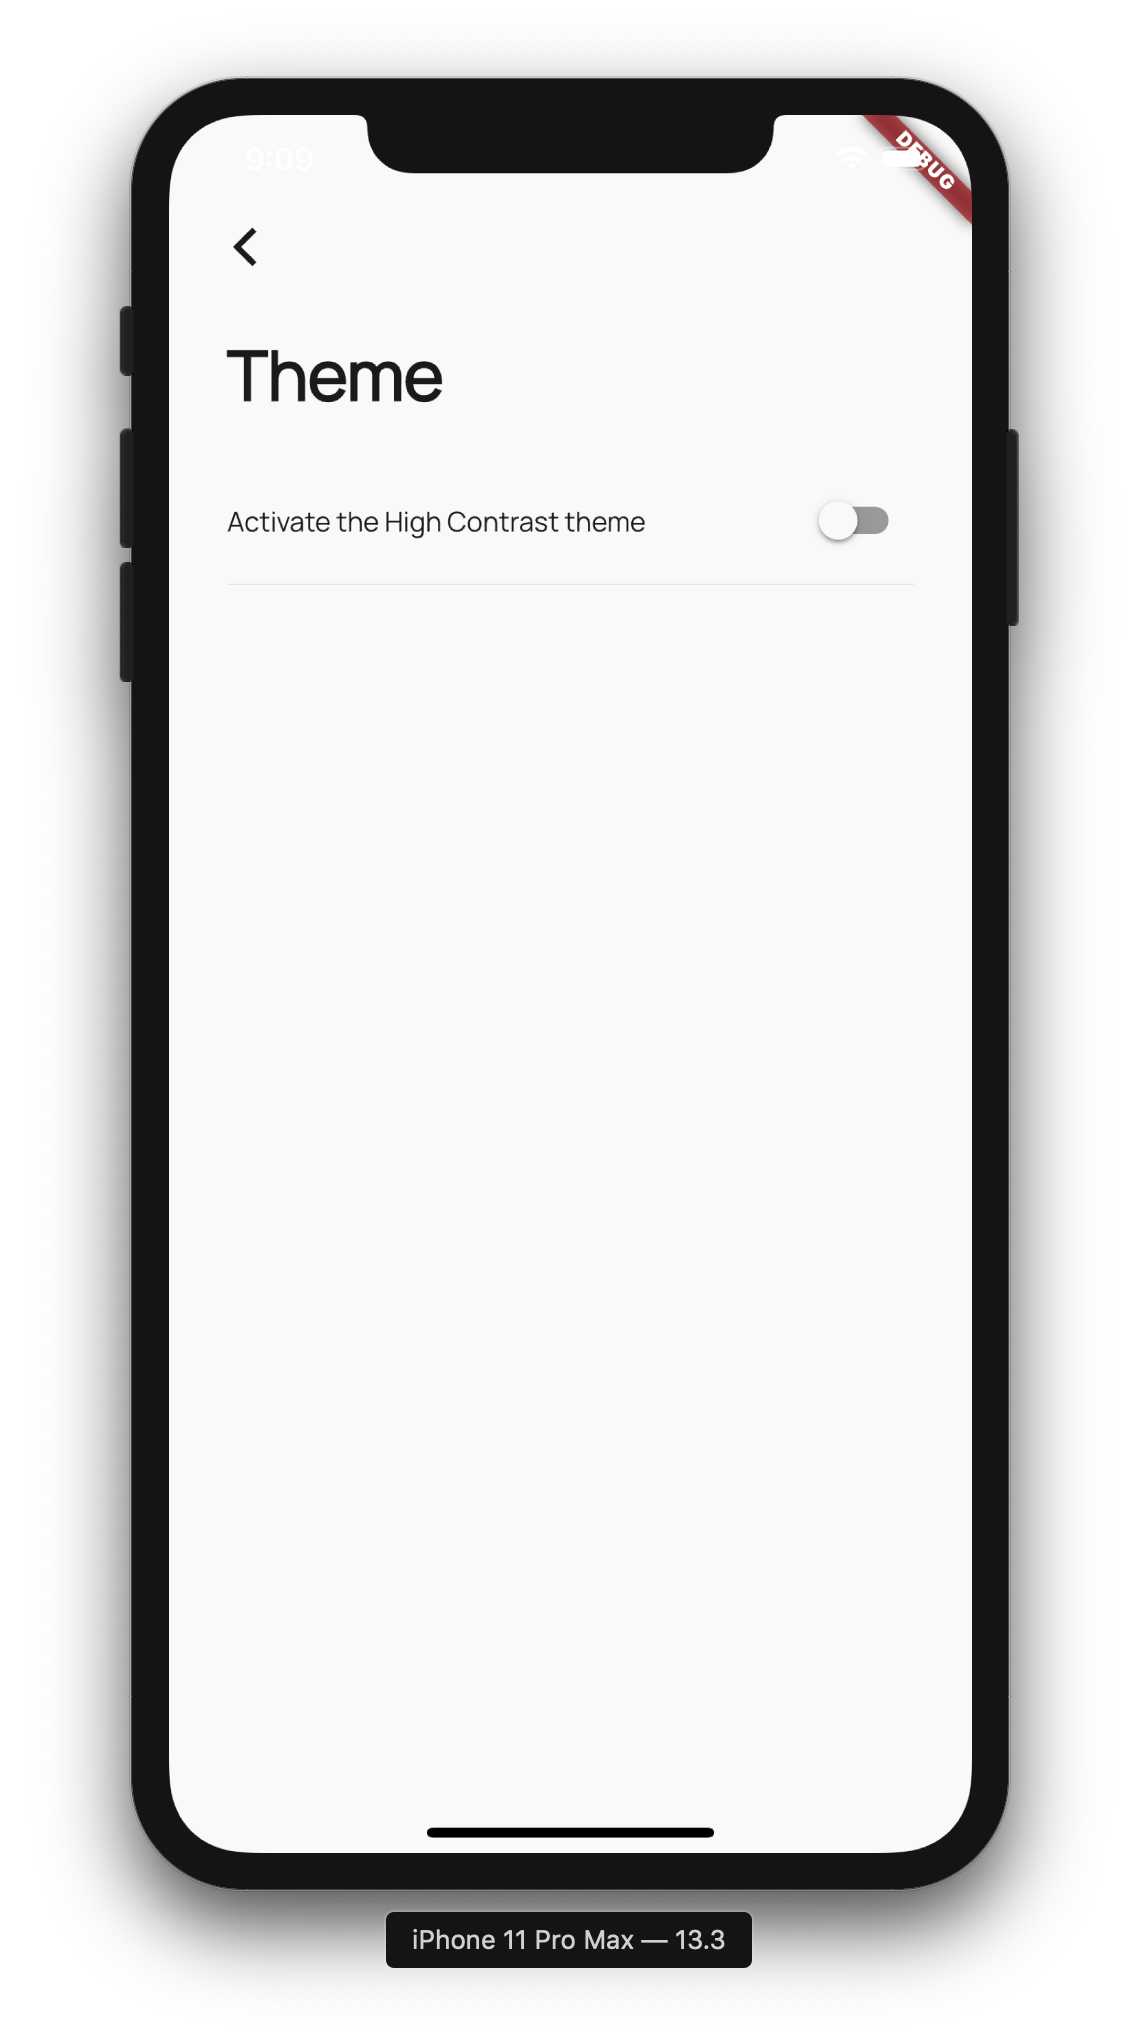
\includegraphics[scale=0.34]{theme_high_contrast_deactivate}
	\caption[Screenshot - Schermata per la scelta del tema]{Screenshot della schermata \textit{Theme}.}\label{xyz}
\end{figure}

È possibile vedere dagli screenshot in Figura 6.18, come si presenta l'applicazione con il tema ad \textit{alto contrasto} attivato. Le schermate \textit{GPS} e \textit{Wind} hanno il medesimo aspetto della schermata \textit{Navigation}.
\begin{figure}[htp]
	\centering
	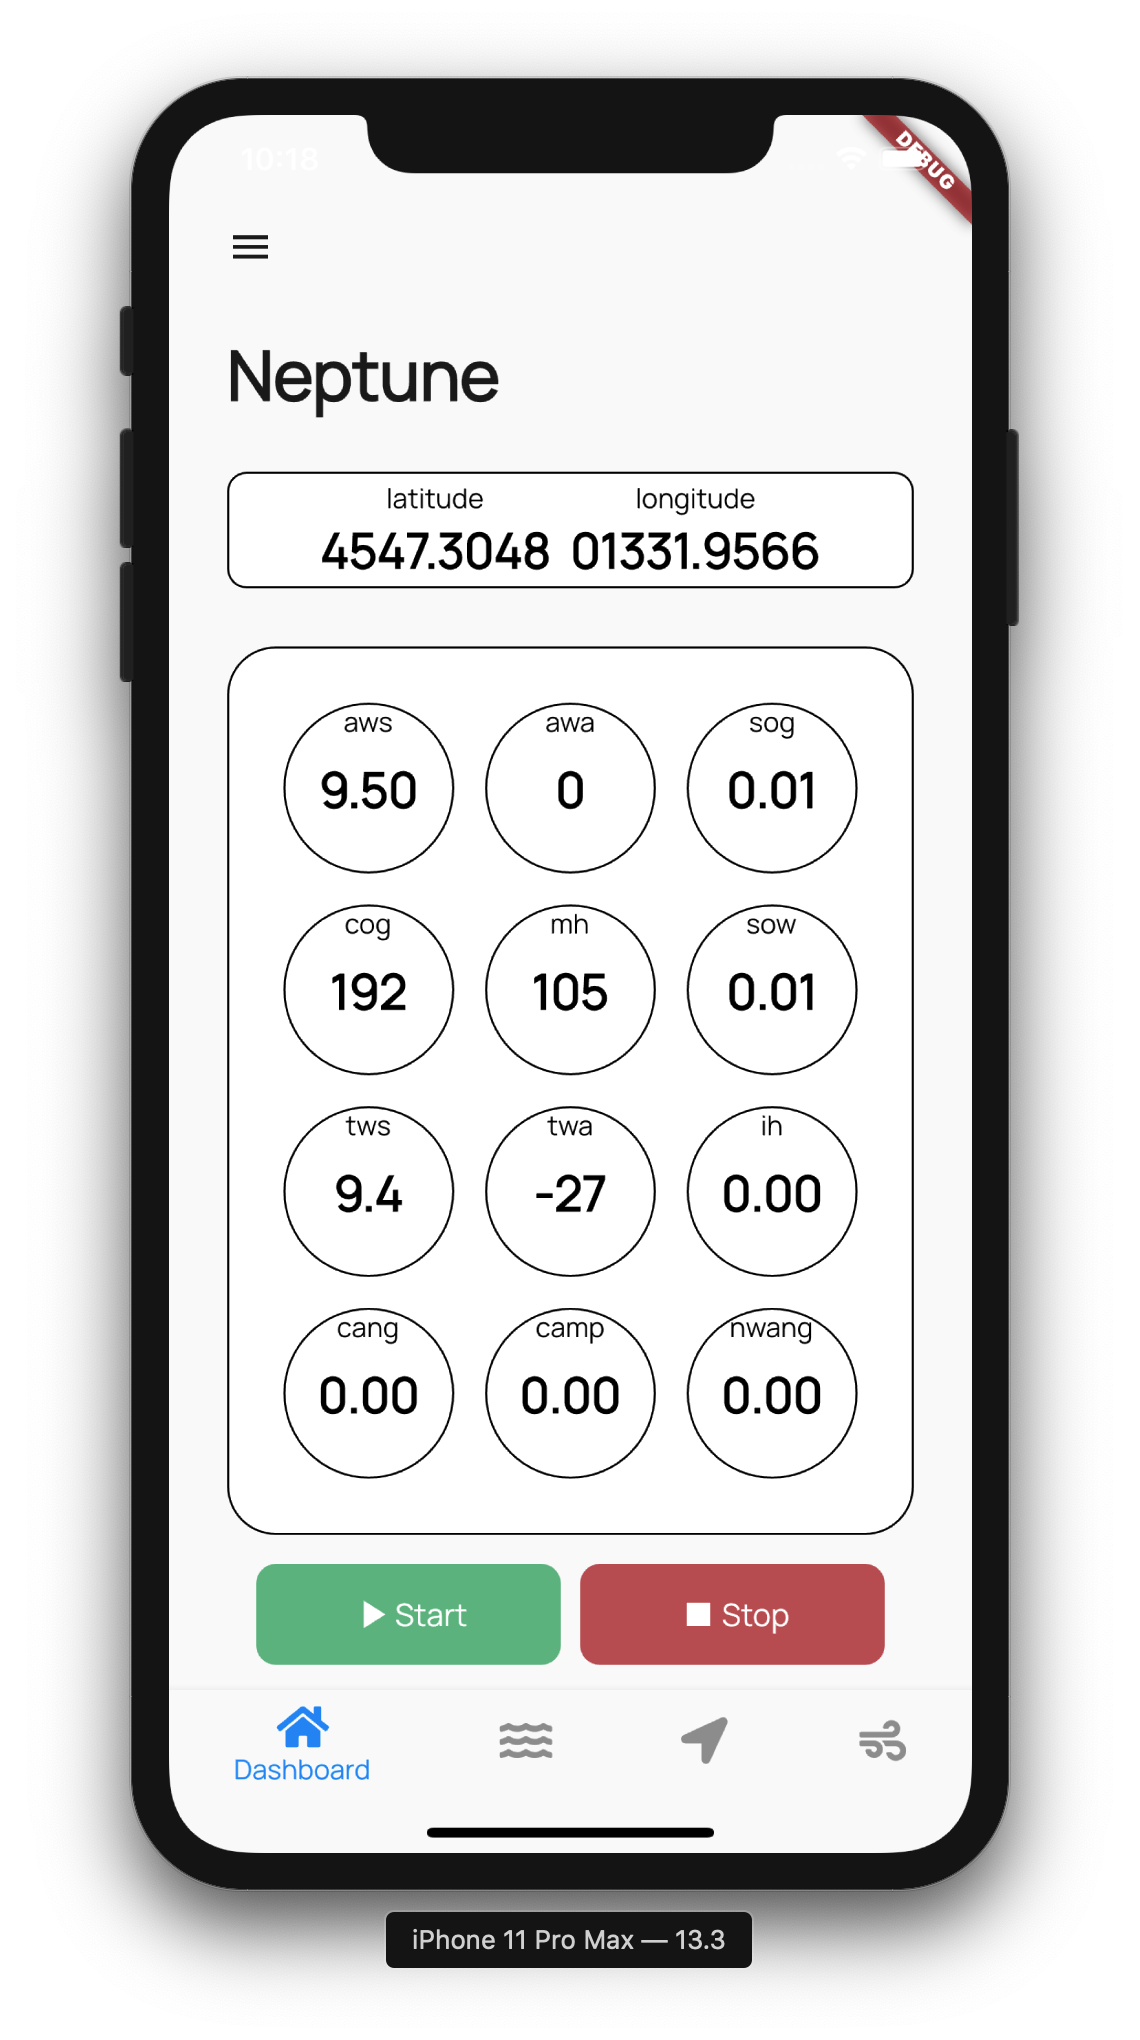
\includegraphics[scale=0.34]{dashboard_high_contrast}
	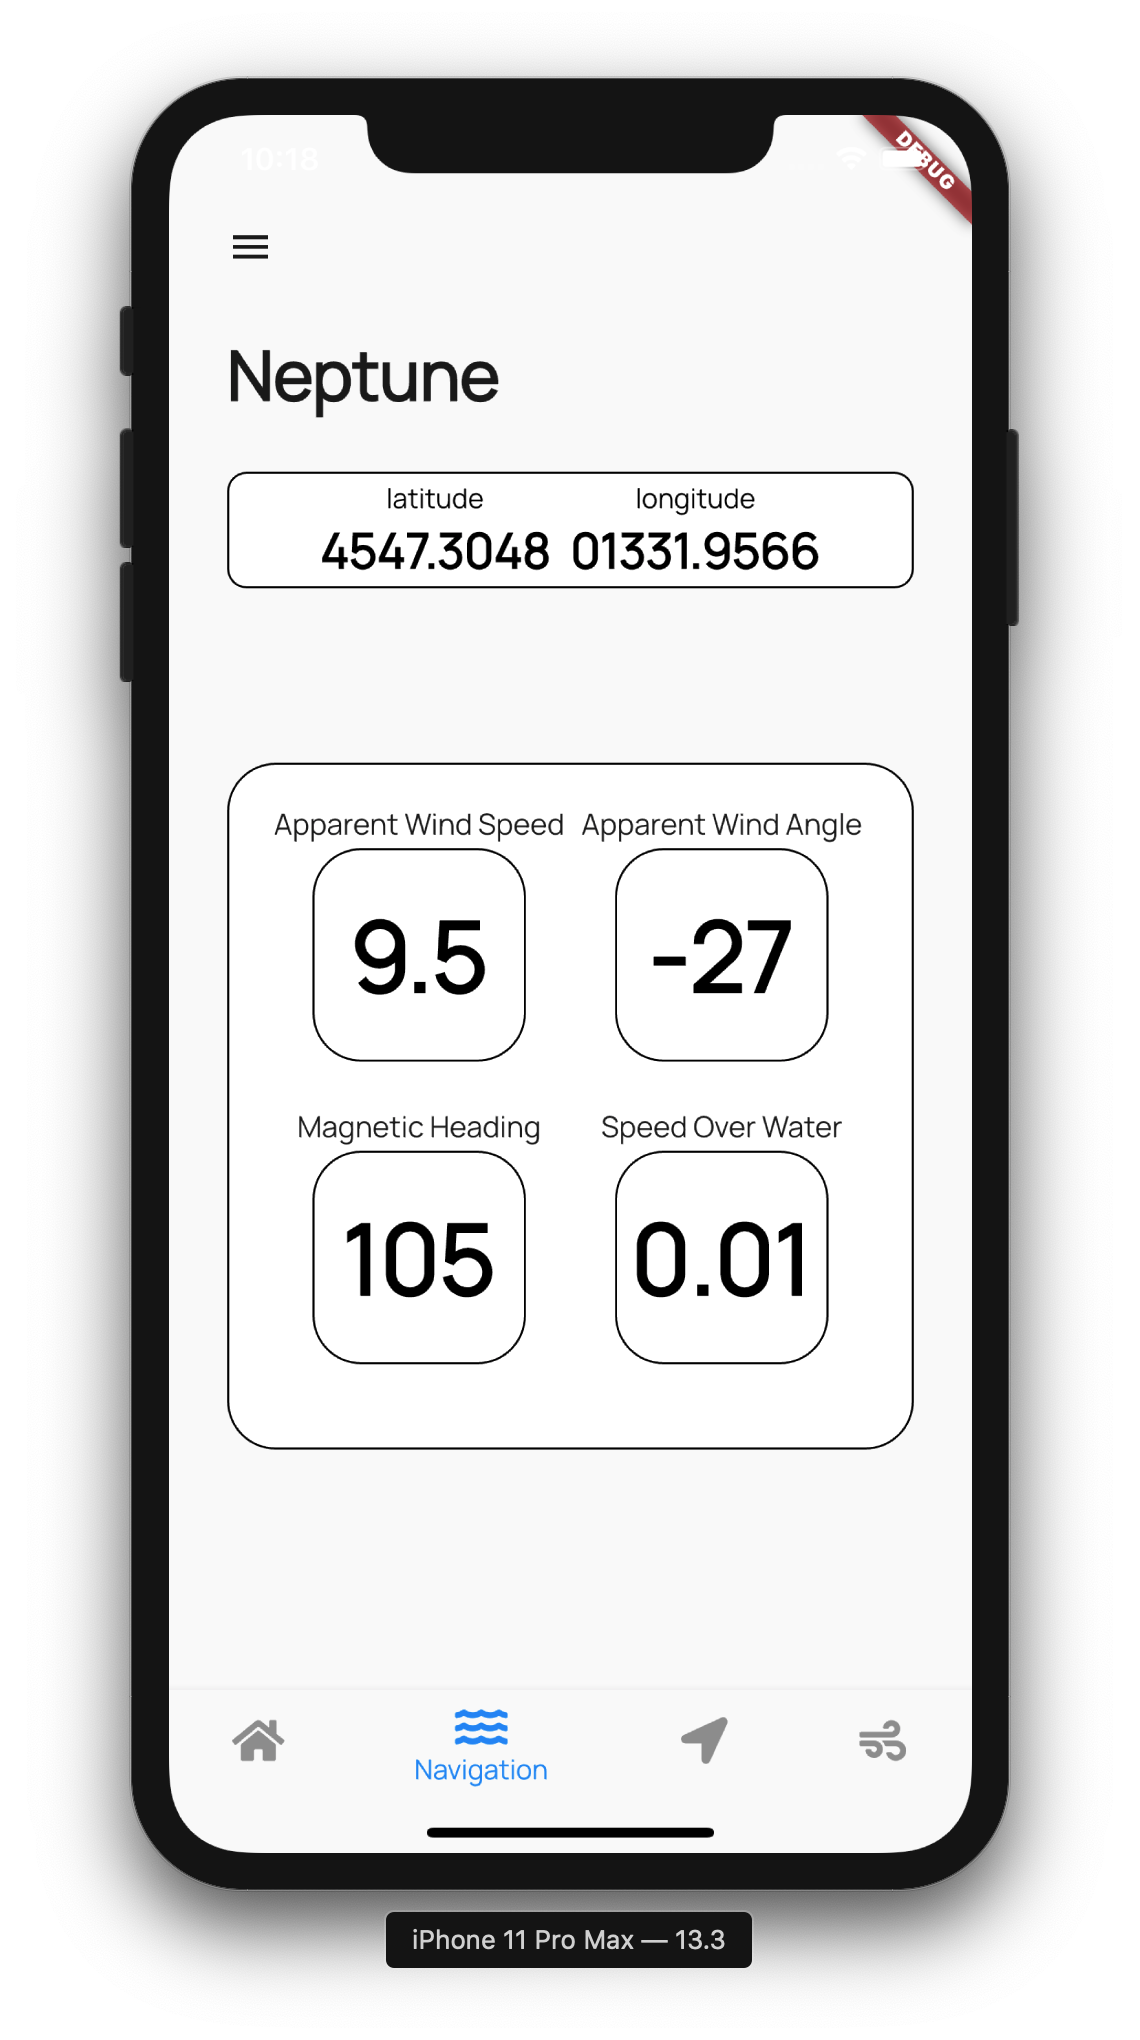
\includegraphics[scale=0.34]{navigation_high_contrast}
	\caption[Screenshot - Dashboard e Navigation con tema ad alto contrasto]{È possibile notare le schermate \textit{Dashboard} e \textit{Navigation} (in ordine da sinistra) con l'applicazione ad \textit{alto contrasto}.}\label{xyz}
\end{figure}

\newpage

\subsection{Widget comuni}
L'interfaccia grafica è stata realizzata utilizzando dei Widget creati \textit{ad-hoc}. Grazie a Flutter e alla flessibilità dell'architettura implementata, questi Widget possono essere aggiunti facilmente in una schermata e risulta molto semplice integrarli, a livello di codice.

\subsubsection{GridBox}
Questo Widget viene utilizzato dalle schermate \textit{Navigation}, \textit{GPS} e \textit{Wind} (Figura 6.19). È un Widget che costruisce una griglia quadrata \verb|2 x 2|, in cui mostrare i dati da monitorare. Gli elementi che compongono la griglia sono stati costruiti per composizione con altri Widget elementari e la loro struttura risulta essere complessa. Tuttavia, la semplicità con cui questo Widget può essere integrato nelle varie schermate rappresenta un grande vantaggio. Tutta la complessità dell'implementazione della griglia è incapsulata all'interno della classe \verb|GridBox|.
Il codice che viene proposto, è stato preso dalla schermata \verb|Navigation|. Dalla riga 11 alla riga 15 è possibile notare la semplicità con cui viene effettuata la chiamata al Widget \verb|GridBox|, passando i relativi parametri, necessari per istanziare correttamente il Widget con dei valori iniziali e per gestire gli aggiornamenti futuri.

\begin{lstlisting}
...

class _NavigationPageState extends State<NavigationPage>
    with AutomaticKeepAliveClientMixin<NavigationPage> {
  @override
  bool get wantKeepAlive => true;

  @override
  Widget build(BuildContext context) {
    super.build(context);
    return GridBox(
      bloc: widget.navigationBloc,
      themeHandler: widget.themeHandler,
      initialData: Navigation(),
    );
  }
}

...
\end{lstlisting}

\begin{figure}
	\begin{center}
		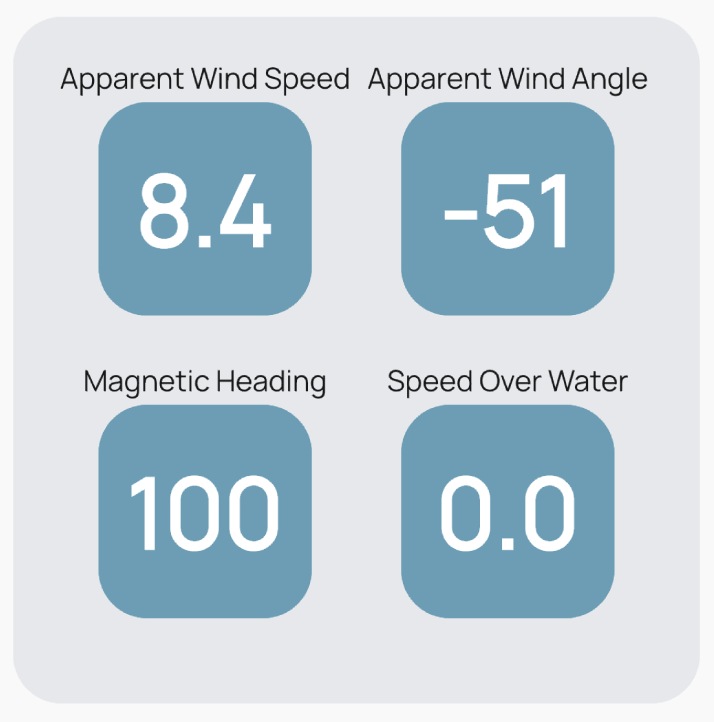
\includegraphics[scale=0.5]{grid_box_widget}
		\caption[Screenshot - GridBox Widget]{Screenshot del Widget \textit{GridBox}. Lo stesso Widget è stato integrato nelle schermate \textit{Navigation}, \textit{GPS} e \textit{Wind}.}
		\label{figura:grid_box_widget}
	\end{center}
\end{figure}

\subsubsection{Location}
\begin{figure}
	\begin{center}
		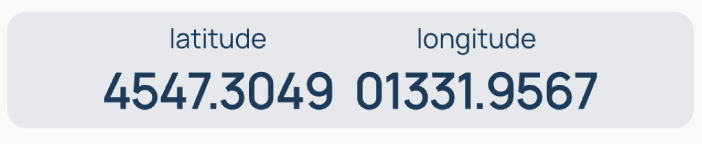
\includegraphics[scale=0.6]{location_widget}
		\caption[Screenshot - Location Widget]{Screenshot del Widget \textit{Location}. Lo stesso Widget è stato integrato in tutte e quattro le schermate.}
		\label{figura:location_widget}
	\end{center}
\end{figure}

Questo Widget permette di visualizzare i dati relativi alla \textit{geolocalizzazione} (Figura 6.20). Il Widget \verb|Location| è presente in tutte le quattro schermate dell'applicazione. È posto nella parte superiore dello schermo, in modo che l'utente possa monitorare continuamente i parametri visualizzati, anche quando passa da una schermata all'altra.

Il codice che verrà illustrato, è stato preso dalla classe \verb|DashboardPage|. Per poter utilizzare questo WIdget bisogna effettuare una chiamata al metodo \verb|create| di \verb|Location| (riga 7). Anche in questo caso, è possibile notare la semplicità con cui i Widget, anche se personalizzati e possiedono una loro logica, possono essere integrati in varie parti dell'applicazione. Infatti, il Widget ha un suo BLoC per interagire con il Repository.

\newpage

\begin{lstlisting}
...
Widget _buildUI() {
    return ListView(
      shrinkWrap: true,
      children: <Widget>[
        LocationWidget.create(context),
        DashboardWidget.create(context),
      ],
    );
  }
...
\end{lstlisting}

\begin{figure}[htp]
	\centering
	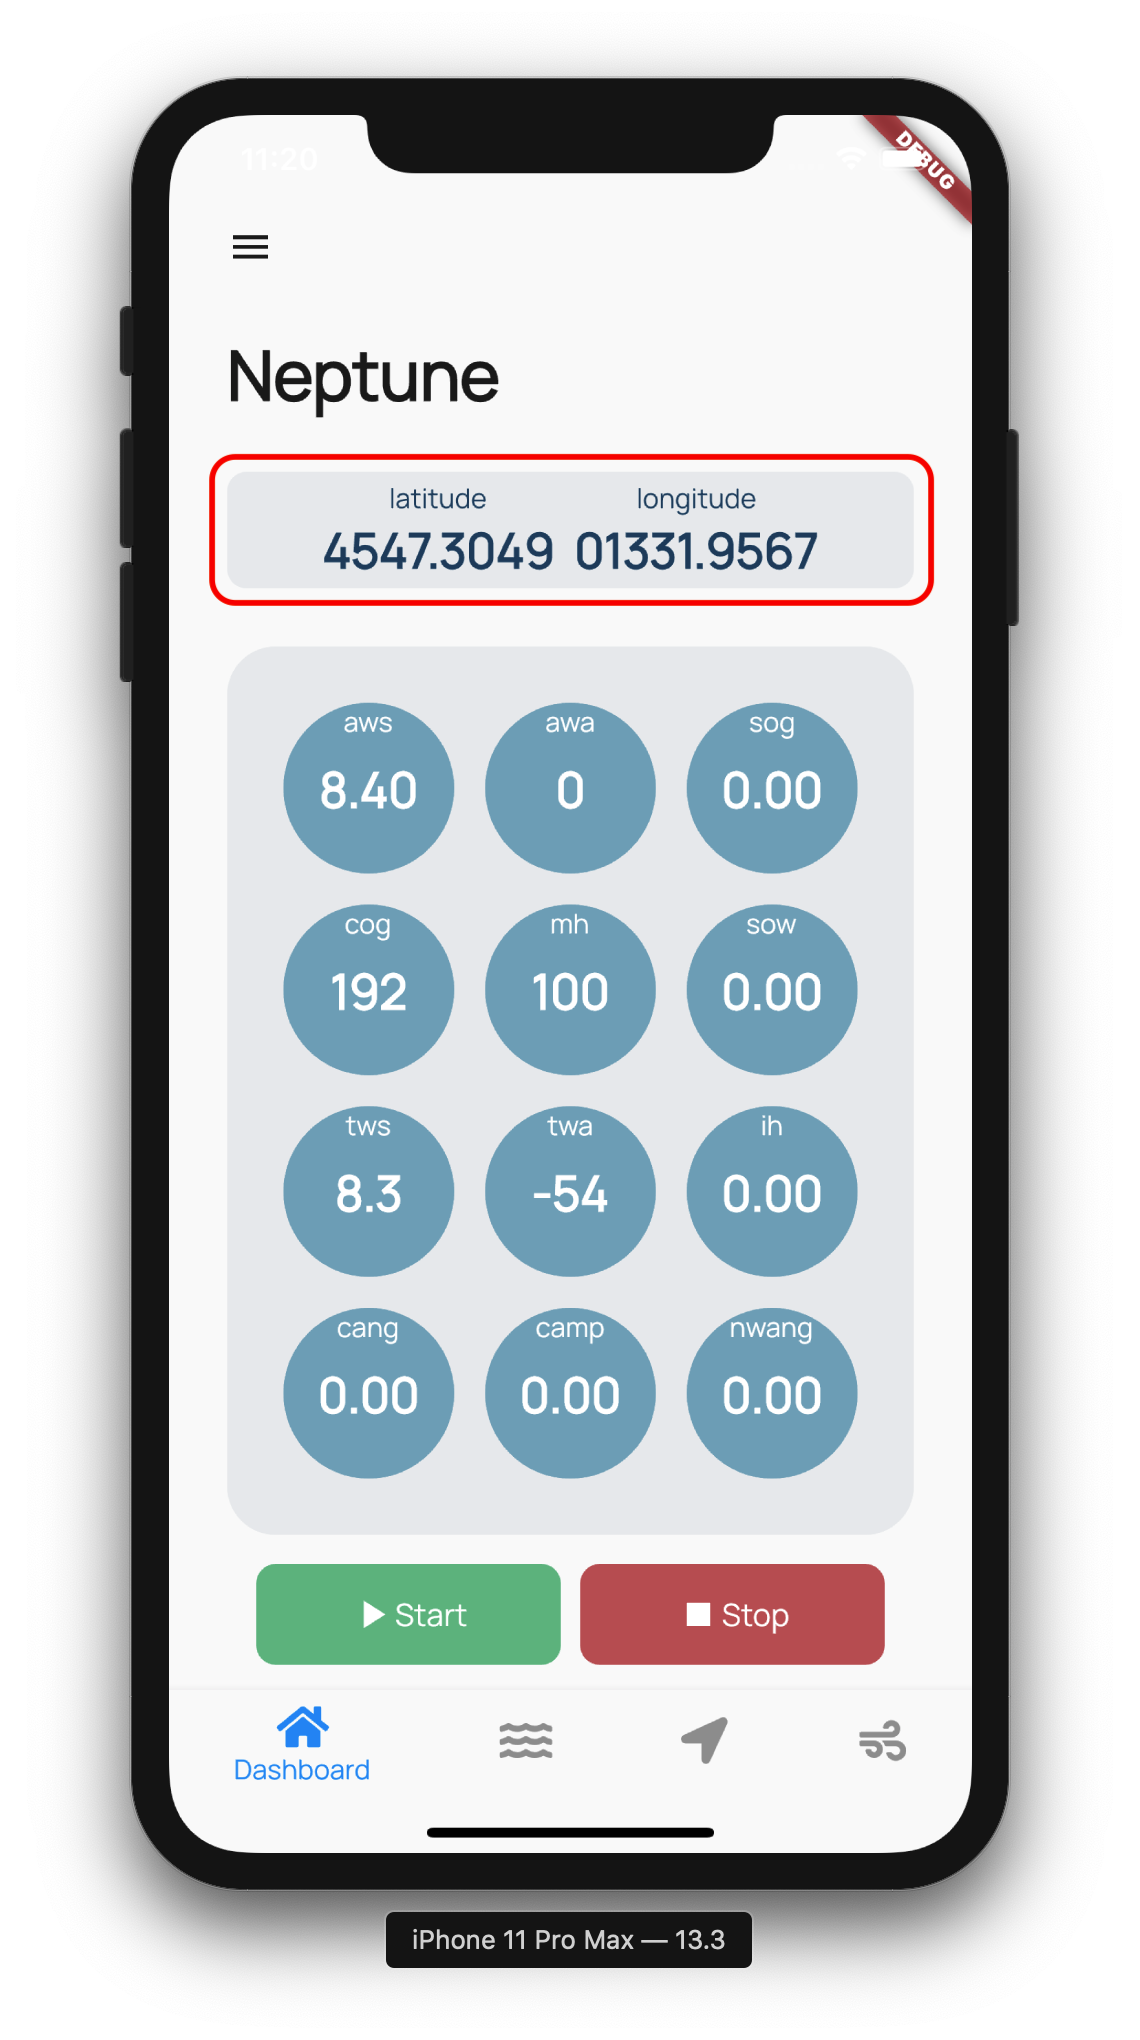
\includegraphics[scale=0.34]{location_widget_dashboard}
	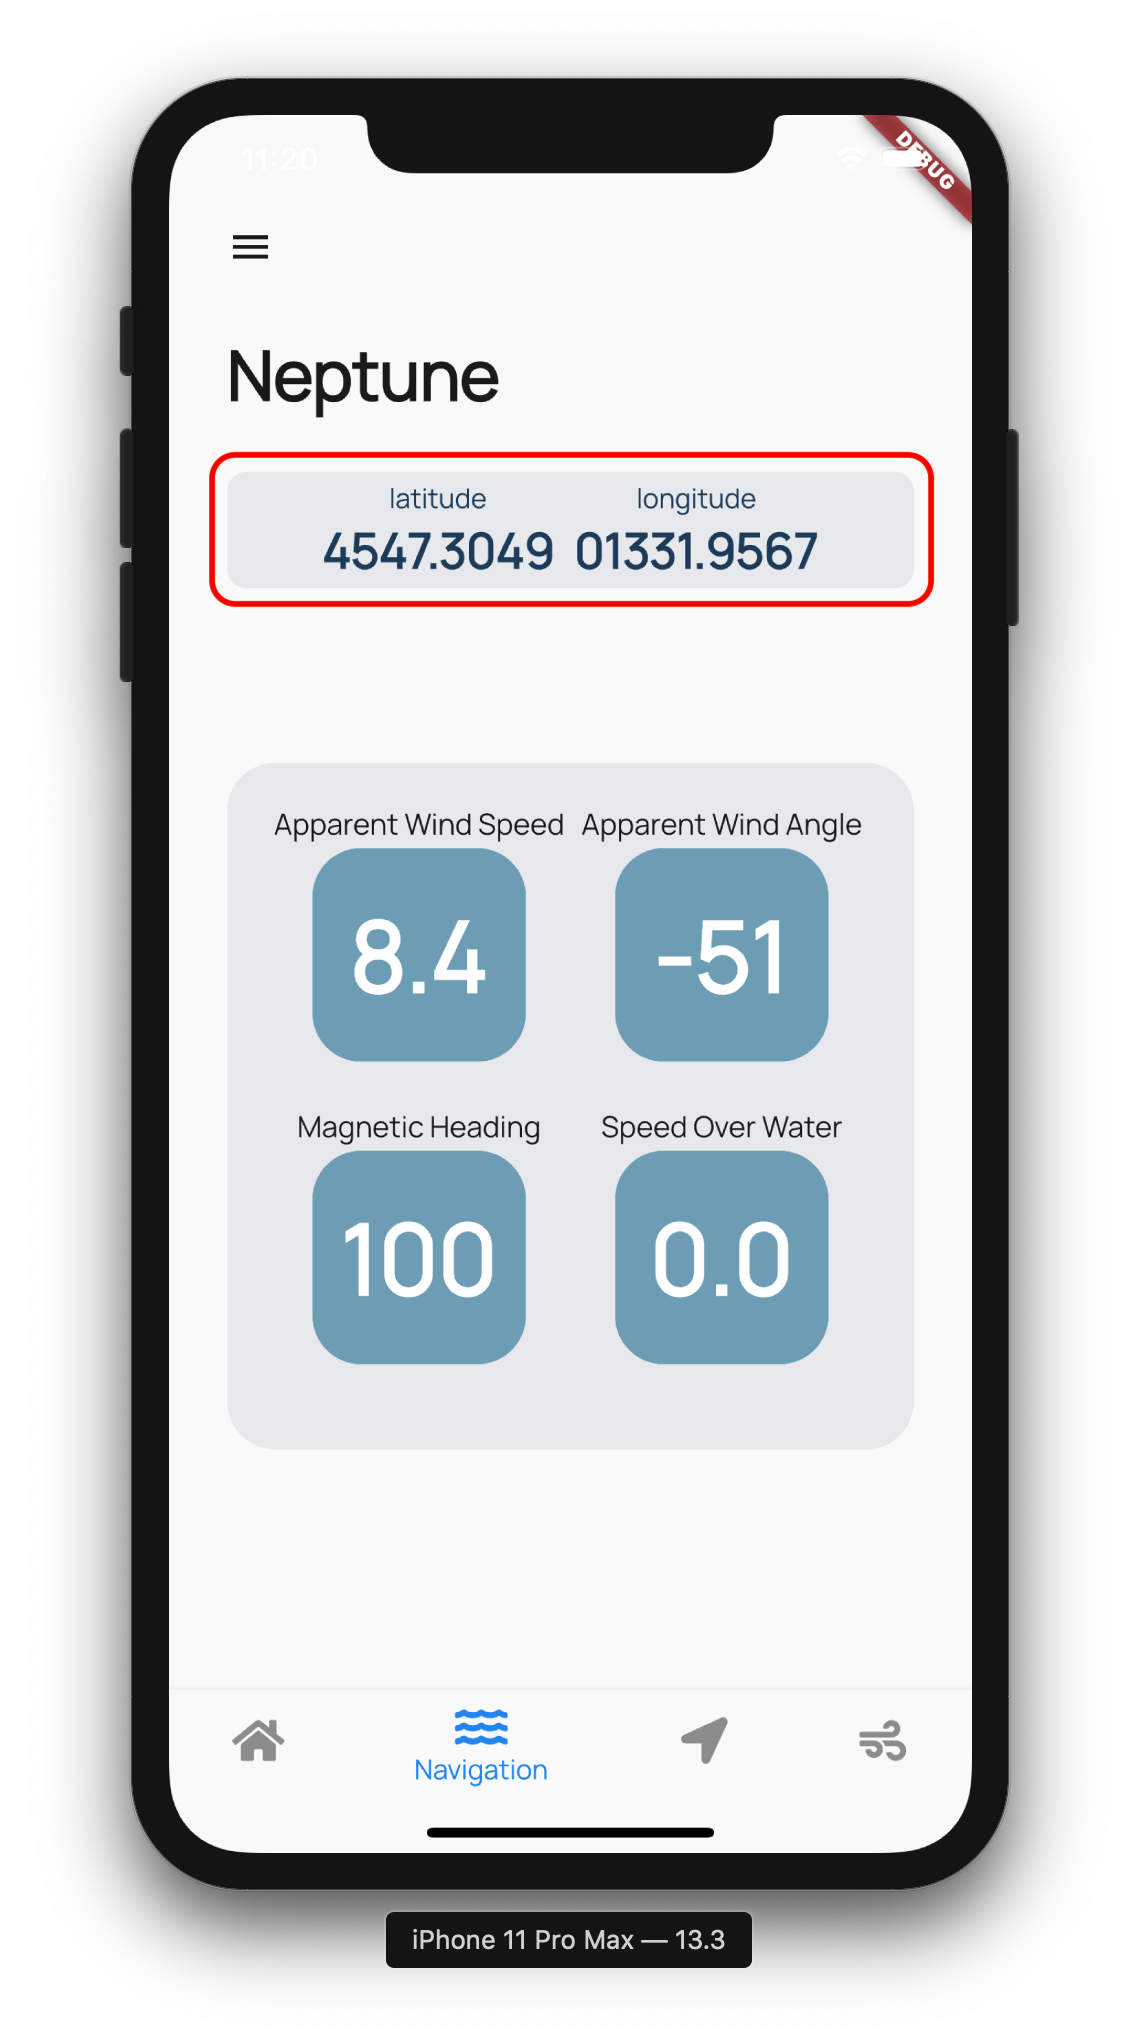
\includegraphics[scale=0.34]{location_widget_navigation}
	\caption[Screenshot - Location Widget nelle schermate Dashboard e Navigation]{Il Widget \textit{Location} nelle schermate \textit{Dashboard} (a sinistra) e \textit{Navigation} (a destra).}\label{xyz}
\end{figure}

\newpage

\subsubsection{Page App Bar}
Questo Widget va a modificare l'\textit{App Bar} di base fornita da Flutter. Questa App Bar viene utilizzata principalmente nelle schermate relative alle impostazioni, quindi nelle schermate \textit{Settings}, \textit{Cache}, \textit{Server} e \textit{Theme}. Lo screen della Figura 6.22 è stato preso dalla schermata \textit{Server}. La flessibilità di questo Widget è data dalla possibilità di modificare il titolo dell'App Bar, in quanto può essere utilizzata, appunto, su molteplici schermate.

\begin{figure}
	\begin{center}
		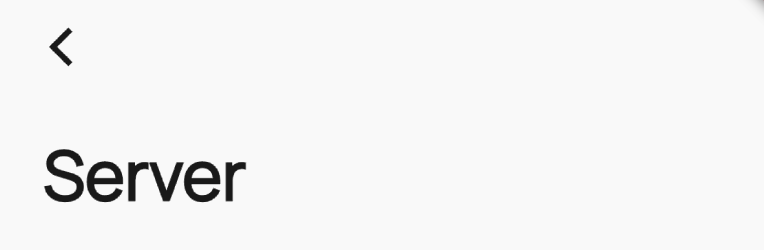
\includegraphics[scale=0.5]{page_app_bar}
		\caption[Screenshot - Page App Bar]{Screenshot del Widget \textit{Page App Bar}. Lo stesso Widget è stato integrato principalmente nelle schermate relative alle impostazioni.}
		\label{figura:page_app_bar}
	\end{center}
\end{figure}

\subsubsection{Sensor Data App Bar}
\verb|Sensor Data App Bar| è un Widget molto simile al precedente (Figura 6.23). Le differenze sostanziali riguardano principalmente gli aspetti grafici. Questo Widget ha la medesima flessibilità del precedente. \verb|Sensor Data App Bar| viene utilizzato nelle schermate dedicate ai dettagli di un dato preciso. Questa funzionalità non è stata implementata, ma ne è stato predisposto l'ambiente.

\begin{figure}
	\begin{center}
		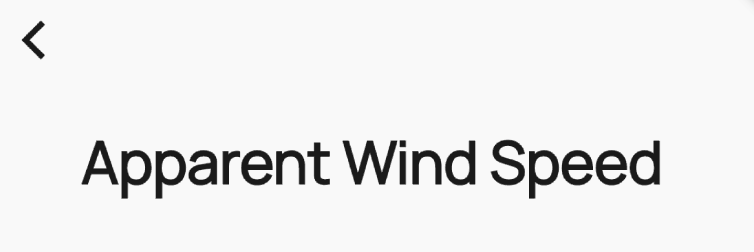
\includegraphics[scale=0.5]{sensor_data_app_bar}
		\caption[Screenshot - Sensor Data App Bar]{Screenshot del Widget \textit{Sensor Data App Bar}. Lo stesso Widget è stato integrato in tutte le schermate che permettono di visualizzare i dettagli di un particolare dato.}
		\label{figura:sensor_data_app_bar}
	\end{center}
\end{figure}

\newpage

\subsection{Palette di colori}
Questa classe fa parte del \textit{package} \verb|utils| e raccoglie tutti i colori personalizzati che sono stati utilizzati nell'applicazione.

Uno dei principali motivi della realizzazione di quest'applicazione era la creazione di un'interfaccia che potesse presentare i dati in maniera più efficace, rivisitando l'aspetto grafico. Pertanto, l'implementazione di questa classe ha un valore importante all'interno del progetto, nonostante non contenga una complessità paragonabile ad altri elementi dell'app.

Di seguito viene mostrato un breve esempio del contenuto di questa classe.

\begin{lstlisting}
...

// Red
static Color redAccent           = Color.fromRGBO(255, 87, 87, 1);
static Color redBackground   = Color.fromRGBO(198, 35, 38, 0.1);
static Color redButton            = Color.fromRGBO(178, 34, 34, 0.7);

...
\end{lstlisting}

\subsection{Temi}
Questa classe è collocata all'interno del package \verb|utils| e permette di gestire il tema dell'applicazione. L'applicazione ha principalmente due temi: 
\begin{enumerate}
	\item \textbf{\textit{default}}: è il tema che si presenta all'apertura dell'applicazione;
	\item \textbf{\textit{alto contrasto}}: è un tema che utilizza soltanto il bianco ed il nero. Questo tema mette in evidenza gli elementi dell'applicazione sopratutto quando il tempo metereologico è soleggiato.
\end{enumerate}

\subsubsection{Themes}
Questa è una semplice classe \textit{enumerazione} in cui vengono elencati i vari nomi dei temi che supporta l'applicazione. Se in futuro verranno realizzati ulteriori temi, sarà necessario aggiornare questa classe.

\begin{lstlisting}
enum Themes {
  DEFAULT,
  HIGH_CONTRAST
}
\end{lstlisting}

\subsubsection{CustomTheme}
\verb|CustomTheme| è un'\textit{interfaccia} (anche se viene dichiarata come una classe astratta, si veda l'Appendice \ref{cap:A} per ulteriori spiegazioni) che fornisce dei metodi comuni per implementare tutti i temi. Di seguito viene presentato l'elenco dei metodi:
\begin{enumerate}
	\item \verb|Color getBackgroundColorOfSensorData()|
	\item \verb|Color getBorderColorOfSensorData()|
	\item \verb|Color getBackgroundColorOfBox()|
	\item \verb|Color getBackgroundBorderOfBox()|
	\item \verb|Color getTextOfSensorValues()|
	\item \verb|Color getTitleTextOfSensorData()|
	\item \verb|Color getTitleTextOfSensorDataInDashboard()|
	\item \verb|Color getTextColorOfLocation()|
\end{enumerate}
È possibile notare che questi metodi vanno ad operare su delle specifiche componenti grafiche o delle parti di essa. Questa interfaccia può essere ampliata per aumentare la personalizzazione grafica dell'applicazione.

\subsubsection{DefaultTheme e HighContrastTheme}
Queste due classi implementano i metodi dell'interfaccia \verb|CustomTheme|. Ciascuna classe va ad applicare dei specifici colori per realizzare un preciso tema. Il \verb|DefaultTheme| utilizza diversi colori, mentre il \verb|HighContrastTheme| utilizza soltanto i colori bianco e nero.

\subsubsection{ThemeHandler}
Anche questa classe implemente l'interfaccia \verb|CustomTheme|, tuttavia non implementa alcun tema. Questa classe, invece, si occupa di applicare il tema, una volta che è stato scelto dall'utente. Infatti, tramite il metodo \verb|applyTheme| è possibile indicare quale tema si vuole applicare. Il metodo in questione, sulla base del parametro ricevuto, istanzia un oggetto che rappresenta il tema scelto e lo applica all'app. Per poter attuare realmente il cambio di tema, questo metodo deve essere chiamato all'interno del metodo \verb|setState(() {})|, in modo da notificare il framework. Così facendo, il framework rileva un cambiamento di stato dell'applicazione e attua le dovute modifiche al Widget tree, visualizzando il tema scelto dall'utente.

Di seguito si mostra l'implementazione del metodo che permette di applicare il tema.
\begin{lstlisting}
void applyTheme(Themes themeChosen) {
    switch (themeChosen) {
      case Themes.DEFAULT:
        _themeChosen = Themes.DEFAULT;
        theme = DefaultTheme();
        break;
      case Themes.HIGH_CONTRAST:
        _themeChosen = Themes.HIGH_CONTRAST;
        theme = HighContrastTheme();
        break;
    }
  }
\end{lstlisting}

\subsection{Main}
Nel file \verb|main.dart| sono contenute tutte le classi fondamentali per il funzionamento dell'applicazione. La struttura iniziale di questo file viene fornita dal framework stesso nel momento in cui viene creato un nuovo progetto in Flutter.

Con la definizione del metodo \verb|void main() => runApp(MyApp())|, viene fatta eseguire l'applicazione, ovvero, viene avviato tutto il processo di inizializzazione delle varie task e del motore di rendering per visualizzare la grafica.

In questo file viene implementata la struttura essenziale su cui si poggia tutta l'applicazione. In particolare:
\begin{enumerate}
	\item Un \verb|FutureBuilder| che va leggere i dati dal file JSON, salvato nella memoria locale del dispositivo, contenente i dati relativi alla connessione al server e al polling;
	\item Il Provider per la gestione dei \textit{temi} (\verb|Provider<ThemeHandler>|);
	\item \verb|MaterialApp| è un \textit{core} Widget che permette di utilizzare tutti i componenti forniti dal framework. In questo Widget vengono anche definite le caratteristiche basilari dell'applicazione come:
	\begin{enumerate}
		\item Il titolo;
		\item Il colore principale;
		\item Il nome dell'applicazione che verrà visualizzato nel menù delle app del dispositivo;
		\item I Widget che andranno a realizzare l'applicazione nel parametro \verb|home|.
	\end{enumerate}
\end{enumerate}

Vengono definiti inoltre degli altri Widget importanti per la struttura essenziale dell'applicazione, come:
\begin{enumerate}
	\item Un'App Bar personalizzata con il nome dell'applicazione;
	\item Una \verb|BottomNavigationBar| che va a definire una barra di navigazione fissa per tutte le schermate principale, posta nella parte inferiore dell'applicazione. Tramite questo Widget, è possibile navigare da una schermata all'altra tra \textit{Dashboard}, \textit{Navigation}, \textit{GPS} e \textit{Wind};
	\item Un \verb|Drawer|, ovvero, un menù laterale che può essere visualizzato facendo uno \textit{swipe} da sinistra a destra, in cui viene illustrata il logo dell'Università degli Studi di Udine e le opzioni;
	\item Il \verb|body| dell'applicazione in questo caso è una \verb|PageView|. La \verb|PageView| è un Widget che permette di organizzare e di navigare tra le varie schermate, scorrendo a destra e a sinistra. Tramite questo Widget viene offerta un ulteriore modalità per navigare tra le schermate, oltre a quella già fornita dalla \verb|BottomNavigationBar|. Nella \verb|PageView|, vengono effettuate tutte le chiamate alle classi delle principali schermate.
\end{enumerate}

\section{Motivazioni delle scelte grafiche implementate}

\subsection{Concetti generali}
Uno degli obiettivi principali della realizzazione di questa applicazione è la completa rivisitazione dell'interfaccia grafica, cercando di sopperire ai difetti strutturali dell'applicazione Web e dell'applicazione Android. Pertanto, il \textbf{layout} dell'applicazione doveva essere particolarmente curato, in modo da comunicare visivamente all'utente una facile comprensione dell'organizzazione degli elementi. Questo aspetto è di fondamentale importanza, in quanto essendo la \textit{competizione} (la regata) il contesto di applicazione di questo software, è assolutamente necessario che l'utente sia in grado di visualizzare immediatamente i dati di cui necessita. Trovandosi in situazioni in cui si devono svolgere manovre di una certa complessità, la squadra deve concentrarsi nel corretto svolgimento di tali manovre, apportando una minore attenzione all'applicazione. L'applicazione deve aiutare la squadra nel rendere l'attività di monitoraggio dei dati il più semplice e fruibile possibile. L'utente non può impiegare troppo tempo nel capire come funziona l'applicazione o nel capire dove deve andare per poter monitorare un particolare dato: il layout deve essere \textbf{intuitivo}. Se così non fosse, l'utente perderebbe troppo tempo a reperire le giuste informazioni e a capire il suo funzionamento, sprecando così del tempo utile per indirizzare correttamente la barca nel percorso prestabilito. Se invece l'applicazione è intuitiva, la squadra ne trarrà vantaggio, in quanto verrà utilizzata attivamente come supporto alle varie decisioni che vengono prese durante tutta la competizione.

\subsection{Scelte stilistiche attuate}
Per ottenere un'interfaccia grafica pulita e facile da utilizzare, nella maggior parte delle schermate si è fatto uso delle \textit{griglie}. Questo elemento grafico va a disporre gli elementi secondo un certo ordine. Tuttavia, la griglia non va a coprire l'intero schermo del dispositivo, ma va coprire la maggior parte dello spazio dello schermo: sia la griglia che il \textit{Location} Widget sono contenuti all'interno di un box di colore grigio. Il significato è quello di delimitare lo spazio di un determinato elemento, da tutto il resto dell'applicazione. In questo modo l'utente, se deve osservare un determinato dato, sa su quale gruppo di elementi deve andare a porre attenzione.

Inoltre, anche gli \textit{spazi bianchi} tra un elemento e l'altro contribuiscono nell'aspetto e nella percezione del layout. Quando si va a sviluppare un layout, si cerca di ottimizzare tutto lo spazio che si ha a disposizione. Questo è un errore che porta alla realizzazione di un'interfaccia grafica molto complessa e caotica. La presenza di molti elementi che possono cambiare forma o contenuto nel tempo (come nel caso dell'applicazione realizzata), può comportare ad un senso di disorientamento e di confusione all'utente. L'utente può trovare difficoltà nel reperire le informazioni corrette con velocità. Riempire lo schermo di elementi grafici implica un \textbf{sovraccarico cognitivo} da parte dell'utente. Questo fenomeno si verifica quando l'utente riceve troppe informazioni e non è in grado di prendere una decisione o di concentrarsi su un'informazione specifica. Se il layout realizzato presenta queste criticità, è necessario riprogettare interamente l'interfaccia, in quanto l'utilizzo di un'applicazione tale, comporterebbe ad ottenere una pessima \textit{user experience}. Nel contesto in cui viene utilizzata l'app, questo potrebbe esporre la squadra anche a dei pericoli: se l'utente non è in grado di focalizzare la sua attenzione sui dati di cui necessita, l'utente non sarà attento né alle manovre della barca, né ai dati forniti dell'applicazione, che potrebbero avvisarlo, ad esempio, di un qualche malfunzionamento del mezzo.

In conclusione, l'organizzazione degli elementi grafici è stata pensata per la realizzazione di un layout che fosse il più pulito ed ordinato possibile, in modo che l'utente possa andare a reperire velocemente i dati, leggerli e confrontarsi con la squadra sulle decisioni da prendere.

\section{Ottimizzazioni}
In questa sezione, si andranno a descrivere le buone pratiche di programmazione in Flutter e le ottimizzazioni attuate nell'applicazione realizzata, per ottenere dei vantaggi a livello di prestazioni e per offrire all'utente un'interfaccia grafica più fluida e reattiva.

\subsection{Provider e StreamBuilder}
Per ottenere delle migliorie dal punto di vista delle prestazioni, è necessario \textit{abbassare} i Provider e gli StreamBuilder nell'albero dei Widget. Se questi Widget vengono posizionati vicini alla radice, nel momento in cui avviene il cambiamento di stato, tutti i loro sotto-alberi vengono aggiornati dal motore di rendering. Quindi, c'è molta probabilità che in una situazione simile, diversi Widget vengano aggiornati anche quando non lo necessitano, sia perché questi sono \textit{immutabili} o perché semplicemente devono essere aggiornati solo alla ricezioni di determinati dati. Risulta \textit{efficiente} dal punto di vista delle prestazioni, posizionare nel punto più basso possibile questi Widget: così facendo, nel momento in cui vengono ricevuti dei dati, vengono aggiornati soltanto i Widget strettamente essenziali. Questa considerazione può sembrare futile, tuttavia è un tema molto importante da considerare dopo aver sviluppato una prima versione del software. Questa problematica può essere fonte di rallentamenti dell'applicazione, in particolare dell'interfaccia grafica. Di conseguenza l'esperienza utente diventa più difficoltosa e spiacevole.

\subsection{Annidamento degli StreamBuilder}
Un altro aspetto molto importante da considerare nella fase di sviluppo dell'applicazione riguarda l'\textit{annidamento} degli StreamBuilder. Come suggerisce il nome, questi Widget sono direttamente collegati a degli \verb|Stream| e nel momento in cui viene ricevuto un nuovo dato tramite questo flusso, il sotto-albero dello \verb|StreamBuilder| (specificato nel parametro \verb|child|) viene aggiornato dal motore di rendering. Pertanto, annidare più \verb|StreamBuilder| tra loro comporta principalmente a:
\begin{enumerate}
	\item \textbf{Aggiornamenti a cascata}: quando uno \verb|StreamBuilder| riceve un nuovo dato, provoca l'aggiornamento di tutti i Widget sottostanti, compresi gli \verb|StreamBuilder| inclusi nel suo sotto-albero. Così facendo, vengono aggiornati a catena tutti gli \verb|StreamBuilder|, provocando diverse chiamate al motore di rendering. Di conseguenza, l'interfaccia risulterà più lenta e meno reattiva alle interazioni dell'utente e farà uno uso maggiore delle risorse del dispositivo;
	\item \textbf{Aggiornamenti non voluti}: un \textit{effetto collaterale} del punto precedente, è che alcuni Widget vengono forzatamente aggiornati anche quando non lo necessitano. Questa casistica è analoga a quella descritta per i Provider.
\end{enumerate}

\subsection{Ottimizzazioni grafiche}

Per ottenere delle ottimizzazioni delle prestazioni nell'interfaccia grafica, è stato utilizzato il metodo statico \verb|Future.microtask(() { ... })|. Flutter, oltre ad avere un \nameref{Event Loop} (Capitolo 4) in cui inserire tutte le \textit{task} che il framework deve elaborare, ha una seconda coda gestita con politica \textit{FIFO}: \textbf{Microtask Queue}. Questa coda viene dedicata allo svolgimento di quelle task che possono essere elaborate e terminate velocemente. Se delle task vengono inserite in questa coda, il framework va ad eseguire prima queste e poi quelle contenute nella \textit{Event Queue} \cite{future_microtask}.

Nell'applicazione, questo meccanismo è stato utilizzato per velocizzare e rendere più fluida l'apertura delle schermate relative ai dati dei sensori e alle impostazioni. In questo modo, quando l'utente vuole andare a modificare le impostazioni della connessione del server, per esempio, il tap dell'utente viene captato e l'evento viene inserito nella \textit{microtask queue}. Il framework si accorge che in questa coda c'è un evento da elaborare, esegue l'elaborazione e torna a controllare se ci sono degli eventuali eventi nella medesima coda o nelle coda degli eventi. Così facendo, l'apertura delle schermate sarà più reattiva.

Il codice illustrato di seguito, è stato preso dalla classe \verb|GridBox|. Dalla riga 7 alla riga 18 è possibile notare l'utilizzo del metodo \verb|Future.microtask()| per l'apertura di una nuova schermata.

\newpage

\begin{lstlisting}
...

Widget _setupBox(String title, String value) {
    return InkWell(
      onTap: () async {
        Future<Widget> buildPageAsync() async {
          return Future.microtask(() {
            return Scaffold(
              appBar: SensorDataAppBar(context: context, 
              title: title),
              body: Column(
                children: <Widget>[
                  Center(
                    child: _buildBox(title, value),
                  ),
                ],
              ),
            );
          });
        }

        Widget page = await buildPageAsync();
        MaterialPageRoute route = MaterialPageRoute(
        builder: (_) => page);
        Navigator.push(context, route);
      },
      child: _buildBox(title, value),
    );
  }
  
...
\end{lstlisting}

\begin{figure}
	\begin{center}
		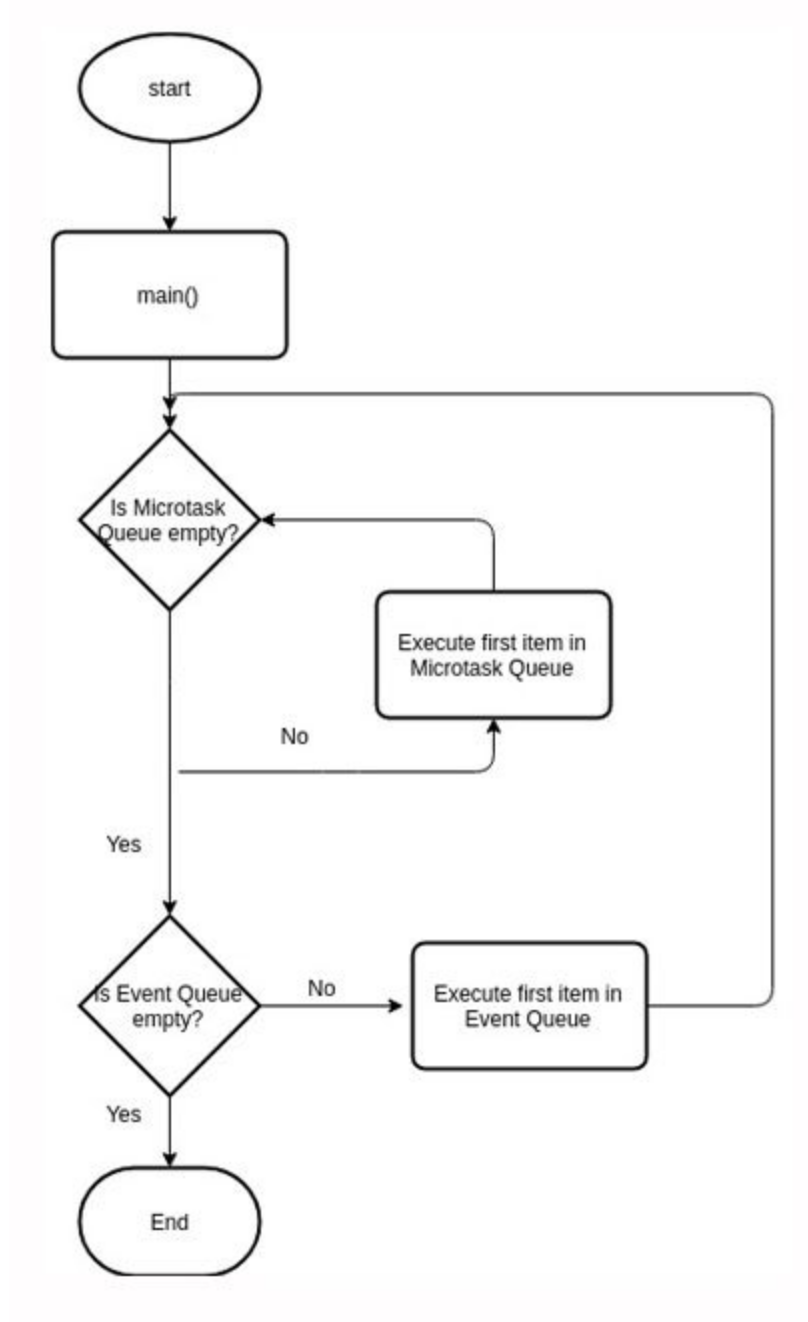
\includegraphics[scale=0.5]{event_queue_microtask_queue}
		\caption[Screenshot - Schema di Event Queue e Microtask Queue]{Uno schema che illustra il funzionamento del meccanismo dell'\textit{Event Queue} e dell'\textit{Microtask Queue}, durante l'esecuzione dell'applicazione \cite{event_queue_microtask_queue}.}
		\label{figura:event_queue_microtask_queue}
	\end{center}
\end{figure}

\chapter{Conclusioni}

\section{Sviluppi futuri}
L'applicazione realizzata ha voluto includere le funzionalità essenziali per poter essere di supporto durante la competizione. Alcune funzionalità sono state aggiunte per poter aumentare la flessibilità dell'applicazione, in modo che possa adattarsi in base alle esigenze: ad esempio, la possibilità di determinare ogni quanti secondi effettuare una connessione al server per ricevere i dati. Inoltre è stata realizzata una grafica ordinata e pulita, in modo da poter individuare immediatamente i dati necessari. Oltre agli aspetti visivi, la gran parte del lavoro è stato fatto nel \textit{background}, ovvero, nella strutturazione di un'architettura che fosse solida e flessibile per poter supportare in futuro delle nuove funzionalità. Pertanto in questa sezione si introducono dei possibili sviluppi futuri, di cui alcuni sono già stati impostati.

\subsection{Notifiche push}
Le \textit{notifiche push} sono una funzionalità peculiare dei dispositivi mobili. Nel contesto d'uso, le notifiche push potrebbero essere utili nel caso in cui si volesse attirare l'attenzione dell'utente per segnalare un determinato evento. Si assuma di trovarsi nel caso in cui l'utente stia monitorando un certo set di dati da una determinata schermata. Se l'applicazione inviasse una notifica push per segnalare, ad esempio, un aumento improvviso della velocità apparente del vento, l'utente se ne accorgerebbe e potrebbe andare nell'apposita schermata per analizzare il dato e verificare se l'avviso ricevuto può essere considerato rilevante o meno.

L'utilizzo delle notifiche push potrebbe essere esteso anche per altre funzionalità in quanto è uno strumento molto flessibile e molto utile.

\begin{figure}[htp]
	\centering
	\includegraphics[scale=0.25]{dashboard_tap}
	\includegraphics[scale=0.25]{dashboard_detail}
	\caption[Sviluppi futuri - Dashboard]{Facendo tap sul dato \textit{aws}, si aprirà la schermata di destra.}\label{xyz}
\end{figure}

\begin{figure}[htp]
	\centering
	\includegraphics[scale=0.25]{location_tap}
	\includegraphics[scale=0.25]{location_detail}
	\includegraphics[scale=0.25]{navigation_tap}
	\includegraphics[scale=0.25]{navigation_detail}
	\caption[Sviluppi futuri - Location e Navigation]{Analogamente per la schermata \textit{Dashboard}, lo stesso avviene sia per il Widget \textit{Location}, sia per la schermata \textit{Navigation} (facendo tap sul dato \textit{Apparent Wind Speed})}\label{xyz}
\end{figure}

\subsection{Grafici e schermate dedicate ai dati}
Una funzionalità molto importante che aiuterebbe l'equipaggio nelle varie decisioni è la realizzazione di una pagina dedicata alla descrizione del dato. Questa funzionalità è stata in parte implementata, ovvero, è già stato predisposto il meccanismo per rilevare l'evento del tocco su un determinato dato e l'apertura della corrispondente schermata. Come si può vedere dagli screenshot, nella fase finale dell'applicazione le schermate sono vuote. Questa funzionalità è già stata predisposta per le schermate \textit{Dashboard}, \textit{Navigation} e per il Widget \textit{Location}. In queste schermate potrebbero essere illustrate delle descrizioni specifiche del dato ed eventualmente uno storico degli eventi riguardo a tale dato. In particolare, per \textit{eventi} si vuole intendere il verificarsi di una forte variazione del valore di un determinato dato, in cui tale variazione risulta essere anomala e può quindi essere motivo di attenzione.

Nella medesima schermata potrebbe essere aggiunto un grafico che illustra tutte le variazioni del dato nel tempo. Il vantaggio di utilizzare questo strumento, permette all'utente di visualizzare in maniera immediata se vi sono state delle variazioni anomale. I grafici possono sfruttare la \textit{cache} che è stata implementata nel \textit{Repository} dell'app. In questo modo, il grafico può attingere i dati da tale fonte.

\subsection{Aggiunta di componenti grafiche}
Per facilitare la fruizione delle informazioni proposte dall'applicazione, sarebbe utile l'implementazione di alcuni componenti grafici dedicati. Ad esempio, potrebbe essere realizzata una \textit{bussola}, con l'utilizzo del giroscopio e dell'accelerometro. La bussola può essere utilizzata per rendersi conto della direzione attuale verso la quale la barca si sta dirigendo.

\subsection{Introduzione di nuovi temi}
L'applicazione così realizzata permette di avere soltanto due temi: \textit{default} e ad \textit{alto contrasto}. Per come è stata strutturata l'applicazione è possibile supportare soltanto due temi. Con delle piccole variazioni al codice, è possibile gestire più temi, in modo che l'utente possa scegliere opportunatamente quello che ritiene più adatto alla situazione in cui si trova.

\subsection{Autenticazione degli utenti}
Aggiungere un servizio di autenticazione degli utenti potrebbe essere utile per capire quali membri della squadra o del team tecnico accedono ai dati e a quali dati. In questo modo è possibile creare un servizio che sia più completo anche dal punto di vista della sicurezza.

\section{Considerazioni sull'approccio cross-platform}
Negli ultimi anni, sempre più aziende cominciano a considerare l'approccio cross-platform come il più conveniente secondo diversi punti di vista. Come è già stato esplicitato durante la tesi, questo approccio è un ottimo compromesso tra \textit{performance}, in quanto questi framework interagiscono nativamente con la componentistica del dispositivo (in particolare con i sensori), e \textit{risorse economiche}. Lo sviluppo di un'applicazione con un framework cross-platform riduce i costi in quanto non è necessario assumere sviluppatori che la realizzino per ogni singola piattaforma e permette all'azienda di affrontare meglio il \textit{time-to-market}. Inoltre vi è un solo codice sorgente che viene gestito da un unico team di sviluppo.

Aziende molto importanti a livello mondiale si sono decise di utilizzare un framework cross-platofrom. In particolare, le aziende che verranno citate hanno sviluppato la loro applicazione utilizzando Flutter \cite{flutter_showcase}:
\begin{enumerate}
	\item \textbf{Alibaba}: uno dei più grandi e-commerce al mondo con milioni di utenti, ha realizzato la sua applicazione mobile per poter acquistare i prodotti offerti;
	\item \textbf{Tencent}: questa azienda ha utilizzato Flutter su molteplici applicazioni. L'azienda fornisce principalmente servizi di intrattenimento (gaming) e di comunicazione (telefonia e messaggistica);
	\item \textbf{New York Times}: ha realizzato un gioco disponibile per Android, iOS, Windows e macOS.
\end{enumerate}

L'aumento dello sviluppo di applicazioni cross-platform è dato principalmente dall'evoluzione tecnologica verificatesi negli ultimi anni: prima i software multipiattaforma non garantivano delle prestazioni e dei risultati paragonabili alle corrispondenti applicazioni native.

\section{Considerazioni su Dart}
Dart è un linguaggio ben strutturato e che si è rivelato flessibile ed efficiente. Personalmente, sono convinto che il successo del linguaggio sia dato proprio dall'esperienza accumulata negli anni da Google, la quale affonda le proprie radici nello sviluppo Web. È un linguaggio che può sostituire JavaScript, sia lato client e sia lato server. A causa della scarsa diffusione, nei primi anni Dart rimase nel buio. Grazie all'avvento di Flutter, gli sviluppatori stanno scoprendo le potenzialità di questo linguaggio, aumentate durante gli anni.

Ho trovato Dart un linguaggio molto flessibile grazie ai molteplici paradigmi che supporta. È molto apprezzabile la vicinanza della sua sintassi a linguaggi come Java e JavaScript, facilitando l'apprendimento del linguaggio. Il linguaggio contiene delle caratteristiche particolari che mi hanno permesso di implementare delle soluzioni eleganti a fronte di determinate problematiche.
Ho particolarmente apprezzato il doppio approccio alla compilazione \textit{AOT} e \textit{JIT}, che permette l’individuazione di errori già in fase di compilazione, riducendo notevolmente il tempo dedicato al \textit{debugging}, senza però privare il linguaggio delle astrazioni che si basano sulla tipizzazione a tempo di esecuzione del codice.

Essendo un Android developer, ho potuto notare le differenze rispetto a \textit{Kotlin}. Dart risulta essere un linguaggio molto più pulito rispetto a Kotlin anche se entrambi hanno di fatto sintassi molto simile e meccanismi comuni, come la tipizzazione \textit{implicita} ed \textit{esplicita}.

Sulla base della mia esperienza sostengo che Google abbia scelto Dart come linguaggio per la realizzazione di applicazioni in Flutter perchè l'azienda aveva già sviluppato delle librerie Web per tale linguaggio, come ad esempio la libreria \textit{Material}. Di conseguenza, risultava più facile realizzare applicazioni in Flutter mediante Dart. Se avessero deciso di utilizzare Kotlin come linguaggio per la scrittura di applicazioni in Flutter, il team di sviluppo avrebbe dovuto svolgere un lavoro ancora più oneroso.

Inoltre, sostengo che il punto a favore che aveva Dart rispetto a Kotlin era più di natura competitiva: Kotlin è un linguaggio nato nel 2011 e sviluppato da un'azienda della Repubblica Ceca, \textit{JetBrains}. Dart invece è stato realizzato direttamente da Google. Di conseguenza, sostengo che la scelta di Dart fosse stata presa anche per non far dipendere il destino del framework da un linguaggio sviluppato da un'azienda esterna a Google.

\section{Considerazioni su Flutter}
Nonostante la giovane età, Flutter sta diventando un punto di riferimento per lo sviluppo di applicazioni cross-platform. Sempre più aziende si avvicinano a questo framework come strumento di sviluppo. LinkedIn, secondo i dati di cui dispone, mostra come Flutter comincia ad essere una \textit{skill} molto richiesta agli sviluppatori in questo periodo e che la richiesta delle aziende a riguardo sta crescendo maggiormente rispetto a tutte le altre tecnologie mobile \cite{flutter_skill}. Un elemento da tenere in considerazione è l'enorme proliferazione di pacchetti e plugin su Pub. Questo significa che c'è un grande interesse attorno a questo framework e mostra anche come Flutter sia costantemente in evoluzione.

Dart si è rivelato essere un ottimo linguaggio per lo sviluppo di applicazioni cross-platform. Un linguaggio molto flessibile e completo in grado di risolvere le problematiche più spinose dello sviluppo mobile. Ritengo che in futuro, il mondo dello sviluppo di applicazioni mobili si polarizzerà principalmente in sostenitori di React Native e di Flutter. React Native e Flutter hanno due caratteristiche che li accomunano e che gli altri framework non possiedono: sono stati sviluppati da due aziende tecnologiche di livello mondiale (rispettivamente, Facebook e Google) e, come conseguenza di questo primo aspetto, hanno molti sviluppatori che sostengono e supportano il framework. Da quest'ultimo punto di vista Flutter è leggermente in svantaggio per il semplice fatto di essere approdato in questo mercato più tardi: sono convinto che nel giro di qualche anno riuscirà superare la metà degli sviluppatori che supporteranno React Native, in virtù anche del futuro sviluppo di Fuchsia.

Inoltre ho particolarmente apprezzato la metodologia utilizzata per realizzare le interfacce grafiche: il meccanismo della composizione dei Widget l'ho trovata affascinante dal punto di vista sia della scrittura ma anche della lettura del codice. Progettare la UI secondo questo approccio permette di produrre del codice molto pulito.

Considero molto positivo l'obiettivo a lungo termine avviato da Google, ovvero, quello di utilizzare Flutter come framework principale per lo sviluppo di applicazioni per \textit{qualsiasi} piattaforma, che questa sia Web, desktop, mobile o il futuro sistema operativo Fuchsia. È una visione molto ampia e di lungo termine che porterà i suoi benefici nei prossimi anni.

\section{Considerazioni personali}

\subsection{Scelta del framework}
Avendo un background come sviluppatore per applicazioni Android, ho particolarmente apprezzato questo framework sopratutto per queste caratteristiche:
\begin{enumerate}
	\item \textbf{Cross-platform}: ho sempre desiderato implementare applicazioni anche per i dispostivi iOS, ma non conoscendo Swift e nemmeno il sistema operativo, ho sempre declinato questa possibilità. Quando scoprii che Flutter era un framework che mi permetteva di realizzare applicazioni per entrambi i sistemi operativi ho subito avuto un forte interessamento ed ho cominciato nel giro di pochi giorni a sviluppare la prima applicazione, grazie anche alla conoscenza accumulata con Java;
	\item \textbf{Prestazioni}: essendo un framework multipiattaforma ho voluto accertarmi che l'applicazione prodotta rispettasse determinati parametri di efficienza e di performance. A seguito di alcuni test svolti sviluppando applicazioni che implementavano funzionalità diverse, ho avuto la possibilità di verificare tali requisiti;
	\item \textbf{Forte tipizzazione}: sviluppando applicazioni per Android, volevo continuare a sviluppare app utilizzando comunque un linguaggio fortemente tipizzato come Java, per poter continuare a trarre tutti i vantaggi dalla forte tipizzazione.
\end{enumerate}

Prima dell'avvento di Flutter ero già a conoscenza della presenza di React Native. Tuttavia, informandomi attraverso le esperienze di alcuni sviluppatori, non mi convinse come framework: alto consumo di memoria centrale, alto consumo di CPU, le prestazioni dell'applicazione non erano ottimali e non si avvicinavano a quelle di un'applicazione nativa. Inoltre, scrivere un'applicazione in React Native produce del codice molto verboso, a differenza di Flutter che produce del codice compatto. Altro aspetto che non mi ha convinto è la presenza del \textit{bridge} JavaScript per interagire con i moduli nativi del dispositivo, il quale rappresenta uno dei principali fattori che contribuisce al degrado complessivo delle prestazioni dell'applicazione.

La facilità nel realizzare delle interfacce grafiche è una ragione che mi ha convinto ancora di più ad adottare questo framework per lo sviluppo di app. Infatti è possibile realizzare UI complesse ma che siano comunque \textit{user-friendly}.

\subsection{Progettazione e sviluppo dell'applicazione}
L'esperienza di tirocinio svolta per lo sviluppo dell'applicazione è stata molto coinvolgente e ricca di spunti per la realizzazione di nuovi progetti in futuro. Mi ha permesso di ampliare le conoscenze riguardo il mondo cross-platform ed il mondo Flutter, permettendomi anche di far tesoro dell'esperienza accumulata durante lo sviluppo di questo progetto. Sono stato particolarmente affascinato dai pattern architetturali disponibili e sostengo che la mia scelta di implementare il pattern \textit{BLoC} sia stata una decisione corretta. È stata una scelta ben ponderata, in quanto volevo costruire una struttura sufficientemente stabile, ma allo stesso tempo, flessibile per poter supportare le funzionalità future che verranno implementate nell'applicazione.

Sono molto soddisfatto di aver fatto esperienza anche nella realizzazione dell'interfaccia grafica, un aspetto un po' carente nel mio bagaglio.

La soddisfazione più grande rimane il fatto di aver realizzato un'applicazione che può essere distribuita sia per Android che per iOS, a partire da un unico codice sorgente. È un risultato che mi rende molto felice e che mi ha particolarmente sorpreso ed entusiasmato. 

Complessivamente, il processo di sviluppo mi ha invogliato molto a superare determinati limiti personali e ad andare oltre a quella \textit{zona di comfort}, per esplorare e apprendere nuove conoscenze. Ritengo che esperienze come questa, debbano essere svolte il più possibile, in quanto permettono alla persona di crescere in modo esponenziale sotto diversi aspetti contemporaneamente: a partire dall'organizzazione del progetto, all'organizzazione dei tempi, delle risorse, all'analisi dei requisiti. Aspetti che vanno ad unire quelle che vengono definite \textit{hard skills} e \textit{soft skills}, entrambe di fondamentale importanza nel mondo dell'innovazione.

\appendix

%%!TEX TS-program = pdflatex
%!TEX root = tesi.tex
%!TEX encoding = UTF-8 Unicode



\chapter{Come si fanno le appendici}
  
    \index{appendici}
    
    Le appendici si fanno con \verb!\appendix! seguito da
    \verb!\chapter{...}!

%%%%%%%%%%%%%%%%%%%%%%

\chapter{Esempi di Citazioni Bibliografiche}
  
    \index{bibliografia}
    \index{citazioni}
    
    P\^{y}r{\l}å in~\cite{pyrl} ha poi
    generalizzato i risultati di
    Bi\v{s}ker~\cite{bisker1}.
    
    Il pacchetto \verb!uniudtesi! carica
    automaticamente \verb!hyperref!\index{ipertesto},
    che a sua volta rende ``cliccabili'' i riferimenti 
    bibliografici nel documento elettronico.

%%%%%%%%%%%%%%%%%%%%%%

\chapter{Ambiente GNU/Linux (ad esempio Ubuntu)}

    \index{Linux}
    
    \begin{flushright}Contributo di\\ Leonardo Taglialegne
    \end{flushright}
    
    Gli ambienti GNU/Linux contengono parecchi strumenti utili per
    la stesura di una tesi di laurea, in particolare segnaliamo:
    \begin{itemize}
     \item Kile
     \item KBibTeX
    \end{itemize}
    Il primo è un editor per il \LaTeX, che include una tabella
    dei simboli, la visualizzazione della struttura, evidenziazione
    del codice e simili comodità, e nelle ultime versioni fornisce
    una visualizzazione in anteprima dei risultati di compilazione.
    
    Il secondo è uno strumento di ricerca, modifica ed inserimento
    di citazioni in formato BibTeX.
    
    I pacchetti relativi (ed altri utili) si installano,
    su ambienti Debian e Ubuntu con:
    \texttt{sudo apt-get install kile kile-l10n kbibtex
           texlive-science \\
           texlive-math-extra texlive-lang-italian }


\chapter{Classi ed interfacce in Dart}
\label{cap:A}
Una peculiarità di questo linguaggio è la definizione delle \textit{interfacce} \cite{implicit_interfaces}. Quando si va a definire una normale classe, questa può essere estesa o implementata da altre classi.
Prendendo l'esempio fornito dalla documentazione ufficiale \cite{implicit_interfaces}:
\begin{lstlisting}
class Person {
  final _name;

  // Not in the interface, since this is a constructor.
  Person(this._name);

  // In the interface.
  String greet(String who) => 'Hello, $who. I am $_name.';
}

class Impostor implements Person {
  get _name => '';

  String greet(String who) => 'Hi $who. Do you know who I am?';
}
\end{lstlisting}

Come è possibile vedere, la classe \verb|Impostor| implementa la classe \verb|Person| e pertanto dovrà implementare tutti i metodi pubblici. Un discorso analogo può essere fatto anche tra \textit{classi astratte} ed interfacce. Si prenda esempio da un caso presente nell'applicazione realizzata:
\begin{lstlisting}
abstract class BaseModel {
  Map<String, dynamic> toMap();
}
\end{lstlisting}

\begin{lstlisting}
class Location extends BaseModel {
  final String latitude;
  final String longitude;

  Location({this.latitude = "0", this.longitude = "0"});

  @override
  Map<String, dynamic> toMap() {
    return null;
  }
}
\end{lstlisting}

Ma è possibile anche implementare la classe \verb|BaseModel|:
\begin{lstlisting}
class Location implements BaseModel {
  final String latitude;
  final String longitude;

  Location({this.latitude = "0", this.longitude = "0"});

  @override
  Map<String, dynamic> toMap() {
    return null;
  }
}
\end{lstlisting}

Dart definisce questo concetto come una \textit{definizione implicita} delle interfacce. Ogni classe definisce implicitamente un'interfaccia contenente tutti i membri dell'istanza della classe e di tutte le interfacce che implementa.

\chapter{AutomaticKeepAliveClientMixin}
\label{cap:B}

Nei linguaggi di programmazione orientati agli oggetti, una \textbf{mixin} è una classe che contiene dei metodi che possono essere utilizzati da parte di altre classi, senza la necessità di dover \textit{estendere} la classe. Il modo in cui le classi ottengono l'accesso ai metodi della mixin dipende dal linguaggio. Una mixin può essere vista come un'interfaccia i cui metodi sono già implementati.

Queste particolari classi vengono ampiamente utilizzate nei linguaggi moderni, sia nei linguaggi che implementano l'\textit{ereditarietà singola}, sia nei linguaggi che supportano l'\textit{ereditarietà multipla}. La problematica principale dell'ereditarietà singola è la mancanza di poter estendere più classi contemporaneamente: questo problema può essere parzialmente risolto con l'utilizzo delle \textit{interfacce}, ma non sempre permettono di ottenere i risultati desiderati. Invece, nonostante l'ereditarietà multipla permetta una maggiore flessibilità nel \textit{riuso del codice}, essa può essere fonte di problemi. In particolare, può verificarsi quello che viene chiamato \textbf{name clash}: è un problema che si verifica quando uno stesso metodo è definito in più \textit{super-classi}. In una situazione del genere, la \textit{sotto-classe} non è in grado di decidere quale metodo ereditare. Sulla base di queste casistiche, l'utilizzo delle mixin si rivela molto utile in quanto permette di aumentare le potenzialità dei linguaggi con ereditarietà singola e di risolvere i problemi causati dall'ereditarietà multipla.

La mixin \verb|AutomaticKeepAliveClientMixin| \cite{keep_alive_mixin} \cite{keep_alive} è una particolare classe che è stata di fondamentale importanza per lo sviluppo dell'applicazione. Questa classe consente ai sotto-alberi di chiedere al framework di essere mantenuti in "\textit{vita}" (\textit{alive}). Tutta la struttura viene mantenuta in vita ogni volta che uno o più discendenti hanno inviato una \verb|KeepAliveNotification|. Per mantenere in "vita", si intende che il framework non deve deallocare o distruggere un determinato oggetto, ma lo deve mantenere attivo, anche se in un dato istante non è strettamente necessario per il proseguimento dell'esecuzione dell'applicazione. Di seguito di introduce un esempio per comprendere meglio l'importante compito di questa classe. Questa mixin è stata di fondamentale importanza per tutte le classi che vanno a comporre l'interfaccia grafica. Infatti, senza l'utilizzo di questa classe, ad ogni cambio di schermata, le pagine che sono state caricate precedentemente, venivano deallocate. Di conseguenza, quando si ritorna su una pagina che era già stata visualizzata precedentemente, questa doveva essere totalmente ricaricata e renderizzata. Tutto questo contribuisce a degradare le prestazioni dell'applicazione e fornisce all'utente una pessima \textit{user experience}. Grazie a questa mixin, invece, la navigazione tra le varie schermate non comporta ad alcun \textit{reload}. Tutte le schermate che sono già state inizializzate, perché l'utente le ha già visionate, vengono mantenute attive in \textit{background}: nel momento in cui l'utente ritorna su una di queste schermate, il framework non fa altro che riprendere l'oggetto già istanziato e proporlo al livello di presentazione. Se l'applicazione non avesse integrato questa mixin, oltre ad avere dei problemi nell'esperienza d'uso, il problema più grave sarebbero stato quello di non fornire un servizio affidabile all'utente, ovvero, il monitoraggio dei dati. Infatti, senza questa mixin, ogni volta che l'utente ritornava su una schermata che aveva già visionato, la schermata doveva essere ricaricata. In quel frangente di tempo necessario per ricaricare e renderizzare nuovamente tutta la schermata, l'applicazione \textit{non visualizza alcun dato}. Quindi, l'applicazione non avrebbe fornito correttamente il servizio per cui era stata progettata. Per questa ragione, durante tutta la spiegazione relativa a questa classe, essa è stata più volte definita come \textit{fondamentale} per la corretta implementazione dell'applicazione.

A livello di codice, \verb|AutomaticKeepAliveClientMixin| viene integrata nella classe come indicato a riga 2, ovvero, con la parola riservata \verb|with|. Questa mixin contiene soltanto un metodo, \verb|wantKeepAlive| (riga 4), necessario per informare il framework se mantenere attiva o meno la schermata. Inoltre, nel corpo del metodo \verb|build| della classe \verb|_NavigationPageState| deve essere aggiunto \verb|super.build(context)| \cite{keep_alive_mixin} (riga 8).


\lstset{numbers=left, % vogliamo numerare le righr
  numberstyle=\tiny, % i numeri sono piccoli
  basicstyle=\ttfamily, % usiamo il carattere dattilografico
  columns=fullflexible, % niente emulazioni di allineamento
  backgroundcolor=\color{lightgray}, % colore di sfondo
  language=Java, % linguaggio usato
  }
  \begin{lstlisting}
class _NavigationPageState extends State<NavigationPage>
    with AutomaticKeepAliveClientMixin<NavigationPage> {
  @override
  bool get wantKeepAlive => true;

  @override
  Widget build(BuildContext context) {
    super.build(context);
    return GridBox(
      bloc: widget.navigationBloc,
      themeHandler: widget.themeHandler,
      initialData: Navigation(),
    );
  }
}
  \end{lstlisting}
  
  


\backmatter

%!TEX TS-program = pdflatex
%!TEX root = tesi.tex
%!TEX encoding = UTF-8 Unicode


\begin{thebibliography}{3}
\selectlanguage{english}
\frenchspacing

\bibitem{regata_costiera}
Regata costiera. \url{https://it.wikipedia.org/wiki/Vela_(sport)#Regate_costiere}, Maggio 2020

\bibitem{vela_sport}
Vela, sport. \url{https://it.wikipedia.org/wiki/Vela_(sport)}, Maggio 2020.

\bibitem{william_b}
Barca a vela da regata \textit{William B}. \url{https://qui.uniud.it/notizieEventi/ricerca-e-innovazione/}, articolo: \textit{Uniud Sailing Lab: ottimi risultati nelle regate autunnali di Lignano Sabbiadoro}. Maggio 2020.

\bibitem{gps}
GPS. \url{https://www.gps.gov/systems/gps/}, Maggio 2020.

\bibitem{statistiche_os_mobile}
Statistiche sull'utilizzo dei sistemi operativi mobili, \url{https://www.statista.com/statistics/272698/global-market-share-held-by-mobile-operating-systems-since-2009/}, Maggio 2020.

\bibitem{google_trends}
Trend dei framework mobile su Google Trends. \url{https://trends.google.it/trends/explore?date=today\%205-y&q=Flutter,React\%20Native,Xamarin,Ionic,NativeScript}, Maggio 2020.

\bibitem{stackoverflow_trends}
Trend dei framework mobile su StackOverflow. \url{https://insights.stackoverflow.com/trends?tags=flutter\%2Creact-native\%2Cxamarin\%2Cionic\%2Ccordova\%2Cnativescript}, Maggio 2020.

\bibitem{grafico_native_hybrid_web}
Grafico illustrativo per le app Native, Hybrid e Web, \url{https://clevertap.com/blog/types-of-mobile-apps/}, Maggio 2020.

\bibitem{considerazioni_native_hybrid_cross_platform}
Considerazioni sull'approccio di sviluppo da utilizzare, \url{https://railsware.com/blog/native-vs-hybrid-vs-cross-platform/}, Maggio 2020.

\bibitem{tasso_di_abbandono_app}
Tasso di abbandono di un'applicazione, \url{https://www.statista.com/statistics/751532/worldwide-application-user-retention-rate/}, Maggio 2020.

\bibitem{mail_google}
Email di un dipendente di Google relativo a \textit{Dash} (Dart). \url{https://gist.github.com/paulmillr/1208618}, Maggio 2020.

\bibitem{pub}
Pub, gestore dei pacchetti in Dart. \url{https://pub.dev/}, Maggio 2020.

\bibitem{confronto_linguaggi}
Homepage di Dart. \url{https://dart.dev/}, Maggio 2020.

\bibitem{tour_linguaggio}
Descrizione del linguaggio Dart. \url{https://dart.dev/guides/language/language-tour}, Maggio 2020.

\bibitem{dart_paradigm}
Elenco dei paradigmi di Dart. \url{https://flutter.dev/docs/resources/faq#what-programming-paradigm-does-flutters-framework-use}, Maggio 2020.

\bibitem{reactive_manifesto}
Reactive Manifesto. \url{https://www.reactivemanifesto.org/}, Maggio 2020.

\bibitem{reactive_programming_wikipedia}
Programmazione reattiva. \url{https://en.wikipedia.org/wiki/Reactive_programming}, Maggio 2020.

\bibitem{aot}
Compilazione anticipata (AOT). \url{https://en.wikipedia.org/wiki/Ahead-of-time_compilation}, Maggio 2020.

\bibitem{codice_intermedio}
Rappresentazione intermedia. \url{https://en.wikipedia.org/wiki/Intermediate_representation#Intermediate_language}, Maggio 2020.

\bibitem{tipizzazione}
Tipizzazione di Dart. \url{https://dart.dev/faq#q-is-dart-a-statically-typed-language}, Maggio 2020.

\bibitem{jit}
Compilazione Just-In-Time (JIT). 
\url{https://en.wikipedia.org/wiki/Just-in-time_compilation}, Maggio 2020.

\bibitem{compilazione_dart}
Piattaforme su cui può essere eseguito il codice Dart. \url{https://dart.dev/platforms}, Maggio 2020.

\bibitem{dartdevc}
Dartdevc. \url{https://dart.dev/tools/dartdevc/faq}, Maggio 2020.

\bibitem{isolate_event_loop}
\textit{Isolate} e \textit{Event Loop}. \url{https://medium.com/dartlang/dart-asynchronous-programming-isolates-and-event-loops-bffc3e296a6a}, Maggio 2020.

\bibitem{isolate_event_loop_youtube}
\textit{Isolate} e \textit{Event Loop}. \url{https://www.youtube.com/watch?v=vl_AaCgudcY}, Maggio 2020.

\bibitem{event_loop}
Event loop. \url{https://webdev-angular3-dartlang-org.firebaseapp.com/articles/performance/event-loop}, Maggio 2020.

\bibitem{future_youtube}
\textit{Future}. \url{https://www.youtube.com/watch?v=OTS-ap9_aXc}, Maggio 2020.

\bibitem{flutter}
Sito ufficiale di Flutter. \url{https://flutter.dev/}, Maggio 2020.

\bibitem{flutter_technical_overview}
Panoramica tecnica di Flutter. \url{https://flutter.dev/docs/resources/technical-overview}, Maggio 2020.

\bibitem{skia}
Skia. \url{https://skia.org/}, Maggio 2020.

\bibitem{hot_reload}
Hot Reload. \url{https://flutter.dev/docs/development/tools/hot-reload}, Maggio 2020.

\bibitem{fuchsia}
Sito ufficiale di Fuchsia. \url{https://fuchsia.dev/}, Maggio 2020.

\bibitem{fuchsia_wikipedia}
Google Fuchsia. \url{https://en.wikipedia.org/wiki/Google_Fuchsia}, Maggio 2020.

\bibitem{fuchsia_google_nest_hub}
Test di Fuchsia su Google Nest Hub. \url{https://www.tomshw.it/}, articolo: \textit{Google Fuchsia si avvicina: l’OS verso l’ultima fase di test interni}. Maggio 2020.

\bibitem{pacchetto_url_launcher}
Pacchetto \verb|url_launcher|. \url{https://pub.dev/packages/url_launcher#-installing-tab-}, Maggio 2020.

\bibitem{redux}
Redux. \url{https://blog.novoda.com/introduction-to-redux-in-flutter/}, Maggio 2020.

\bibitem{provider_first}
Provider. \url{https://medium.com/flutter-community/understanding-provider-in-diagrams-part-1-providing-values-4379aa1e7fd5}, Maggio 2020.

\bibitem{presentazione_bloc}
Prima presentazione del pattern BLoC. \url{https://www.youtube.com/watch?v=PLHln7wHgPE}, Maggio 2020.

\bibitem{repository_pattern}
Repository pattern. \url{http://hannesdorfmann.com/android/evolution-of-the-repository-pattern}, Maggio 2020.

\bibitem{architettura_implementata}
Architettura implementata. \url{https://www.toptal.com/cross-platform/code-sharing-angular-dart-flutter-bloc}, Maggio 2020.

\bibitem{connectivity_plugin}
Pacchetto \verb|connectivity 0.4.8+2|. \url{https://pub.dev/packages/connectivity/versions/0.4.8+2}, Giugno 2020.

\bibitem{future_microtask}
Future Microtask. \url{https://www.woolha.com/tutorials/dart-how-to-schedule-a-microtask}, Giugno 2020.

\bibitem{event_queue_microtask_queue}
Schema Event Queue e Microtask Queue. \url{https://www.woolha.com/articles/dart-event-loop-microtask-event-queue}, Giugno 2020.

\bibitem{flutter_showcase}
Aziende che utilizzano Flutter. \url{https://flutter.dev/showcase}, Maggio 2020.

\bibitem{flutter_skill}
L'abilità di sviluppare applicazioni in Flutter è la skill più richiesta nell'ultimo periodo. \url{https://learning.linkedin.com/blog/tech-tips/the-fastest-growing-skills-among-software-engineers--and-how-to-}, Maggio 2020.

\bibitem{implicit_interfaces}
Interfacce implicite in Dart. \url{https://dart.dev/guides/language/language-tour#implicit-interfaces}, Giugno 2020.

\bibitem{keep_alive_mixin}
\verb|AutomaticKeepAliveClientMixin|. \url{https://api.flutter.dev/flutter/widgets/AutomaticKeepAliveClientMixin-mixin.html}, Giugno 2020.

\bibitem{keep_alive}
\verb|AutomaticKeepAlive|. \url{https://api.flutter.dev/flutter/widgets/AutomaticKeepAlive-class.html}, Giugno 2020.

\end{thebibliography}
\selectlanguage{italian}
\nonfrenchspacing

%!TEX encoding = UTF-8 Unicode\printindex % se si fa l'indice analitico.

\end{document}
